% Options for packages loaded elsewhere
% Options for packages loaded elsewhere
\PassOptionsToPackage{unicode}{hyperref}
\PassOptionsToPackage{hyphens}{url}
\PassOptionsToPackage{dvipsnames,svgnames,x11names}{xcolor}
%
\documentclass[
  letterpaper,
  DIV=11,
  numbers=noendperiod,
  oneside]{scrreprt}
\usepackage{xcolor}
\usepackage[left=1in,marginparwidth=2.0666666666667in,textwidth=4.1333333333333in,marginparsep=0.3in]{geometry}
\usepackage{amsmath,amssymb}
\setcounter{secnumdepth}{5}
\usepackage{iftex}
\ifPDFTeX
  \usepackage[T1]{fontenc}
  \usepackage[utf8]{inputenc}
  \usepackage{textcomp} % provide euro and other symbols
\else % if luatex or xetex
  \usepackage{unicode-math} % this also loads fontspec
  \defaultfontfeatures{Scale=MatchLowercase}
  \defaultfontfeatures[\rmfamily]{Ligatures=TeX,Scale=1}
\fi
\usepackage{lmodern}
\ifPDFTeX\else
  % xetex/luatex font selection
\fi
% Use upquote if available, for straight quotes in verbatim environments
\IfFileExists{upquote.sty}{\usepackage{upquote}}{}
\IfFileExists{microtype.sty}{% use microtype if available
  \usepackage[]{microtype}
  \UseMicrotypeSet[protrusion]{basicmath} % disable protrusion for tt fonts
}{}
\makeatletter
\@ifundefined{KOMAClassName}{% if non-KOMA class
  \IfFileExists{parskip.sty}{%
    \usepackage{parskip}
  }{% else
    \setlength{\parindent}{0pt}
    \setlength{\parskip}{6pt plus 2pt minus 1pt}}
}{% if KOMA class
  \KOMAoptions{parskip=half}}
\makeatother
% Make \paragraph and \subparagraph free-standing
\makeatletter
\ifx\paragraph\undefined\else
  \let\oldparagraph\paragraph
  \renewcommand{\paragraph}{
    \@ifstar
      \xxxParagraphStar
      \xxxParagraphNoStar
  }
  \newcommand{\xxxParagraphStar}[1]{\oldparagraph*{#1}\mbox{}}
  \newcommand{\xxxParagraphNoStar}[1]{\oldparagraph{#1}\mbox{}}
\fi
\ifx\subparagraph\undefined\else
  \let\oldsubparagraph\subparagraph
  \renewcommand{\subparagraph}{
    \@ifstar
      \xxxSubParagraphStar
      \xxxSubParagraphNoStar
  }
  \newcommand{\xxxSubParagraphStar}[1]{\oldsubparagraph*{#1}\mbox{}}
  \newcommand{\xxxSubParagraphNoStar}[1]{\oldsubparagraph{#1}\mbox{}}
\fi
\makeatother

\usepackage{color}
\usepackage{fancyvrb}
\newcommand{\VerbBar}{|}
\newcommand{\VERB}{\Verb[commandchars=\\\{\}]}
\DefineVerbatimEnvironment{Highlighting}{Verbatim}{commandchars=\\\{\}}
% Add ',fontsize=\small' for more characters per line
\usepackage{framed}
\definecolor{shadecolor}{RGB}{241,243,245}
\newenvironment{Shaded}{\begin{snugshade}}{\end{snugshade}}
\newcommand{\AlertTok}[1]{\textcolor[rgb]{0.68,0.00,0.00}{#1}}
\newcommand{\AnnotationTok}[1]{\textcolor[rgb]{0.37,0.37,0.37}{#1}}
\newcommand{\AttributeTok}[1]{\textcolor[rgb]{0.40,0.45,0.13}{#1}}
\newcommand{\BaseNTok}[1]{\textcolor[rgb]{0.68,0.00,0.00}{#1}}
\newcommand{\BuiltInTok}[1]{\textcolor[rgb]{0.00,0.23,0.31}{#1}}
\newcommand{\CharTok}[1]{\textcolor[rgb]{0.13,0.47,0.30}{#1}}
\newcommand{\CommentTok}[1]{\textcolor[rgb]{0.37,0.37,0.37}{#1}}
\newcommand{\CommentVarTok}[1]{\textcolor[rgb]{0.37,0.37,0.37}{\textit{#1}}}
\newcommand{\ConstantTok}[1]{\textcolor[rgb]{0.56,0.35,0.01}{#1}}
\newcommand{\ControlFlowTok}[1]{\textcolor[rgb]{0.00,0.23,0.31}{\textbf{#1}}}
\newcommand{\DataTypeTok}[1]{\textcolor[rgb]{0.68,0.00,0.00}{#1}}
\newcommand{\DecValTok}[1]{\textcolor[rgb]{0.68,0.00,0.00}{#1}}
\newcommand{\DocumentationTok}[1]{\textcolor[rgb]{0.37,0.37,0.37}{\textit{#1}}}
\newcommand{\ErrorTok}[1]{\textcolor[rgb]{0.68,0.00,0.00}{#1}}
\newcommand{\ExtensionTok}[1]{\textcolor[rgb]{0.00,0.23,0.31}{#1}}
\newcommand{\FloatTok}[1]{\textcolor[rgb]{0.68,0.00,0.00}{#1}}
\newcommand{\FunctionTok}[1]{\textcolor[rgb]{0.28,0.35,0.67}{#1}}
\newcommand{\ImportTok}[1]{\textcolor[rgb]{0.00,0.46,0.62}{#1}}
\newcommand{\InformationTok}[1]{\textcolor[rgb]{0.37,0.37,0.37}{#1}}
\newcommand{\KeywordTok}[1]{\textcolor[rgb]{0.00,0.23,0.31}{\textbf{#1}}}
\newcommand{\NormalTok}[1]{\textcolor[rgb]{0.00,0.23,0.31}{#1}}
\newcommand{\OperatorTok}[1]{\textcolor[rgb]{0.37,0.37,0.37}{#1}}
\newcommand{\OtherTok}[1]{\textcolor[rgb]{0.00,0.23,0.31}{#1}}
\newcommand{\PreprocessorTok}[1]{\textcolor[rgb]{0.68,0.00,0.00}{#1}}
\newcommand{\RegionMarkerTok}[1]{\textcolor[rgb]{0.00,0.23,0.31}{#1}}
\newcommand{\SpecialCharTok}[1]{\textcolor[rgb]{0.37,0.37,0.37}{#1}}
\newcommand{\SpecialStringTok}[1]{\textcolor[rgb]{0.13,0.47,0.30}{#1}}
\newcommand{\StringTok}[1]{\textcolor[rgb]{0.13,0.47,0.30}{#1}}
\newcommand{\VariableTok}[1]{\textcolor[rgb]{0.07,0.07,0.07}{#1}}
\newcommand{\VerbatimStringTok}[1]{\textcolor[rgb]{0.13,0.47,0.30}{#1}}
\newcommand{\WarningTok}[1]{\textcolor[rgb]{0.37,0.37,0.37}{\textit{#1}}}

\usepackage{longtable,booktabs,array}
\usepackage{calc} % for calculating minipage widths
% Correct order of tables after \paragraph or \subparagraph
\usepackage{etoolbox}
\makeatletter
\patchcmd\longtable{\par}{\if@noskipsec\mbox{}\fi\par}{}{}
\makeatother
% Allow footnotes in longtable head/foot
\IfFileExists{footnotehyper.sty}{\usepackage{footnotehyper}}{\usepackage{footnote}}
\makesavenoteenv{longtable}
\usepackage{graphicx}
\makeatletter
\newsavebox\pandoc@box
\newcommand*\pandocbounded[1]{% scales image to fit in text height/width
  \sbox\pandoc@box{#1}%
  \Gscale@div\@tempa{\textheight}{\dimexpr\ht\pandoc@box+\dp\pandoc@box\relax}%
  \Gscale@div\@tempb{\linewidth}{\wd\pandoc@box}%
  \ifdim\@tempb\p@<\@tempa\p@\let\@tempa\@tempb\fi% select the smaller of both
  \ifdim\@tempa\p@<\p@\scalebox{\@tempa}{\usebox\pandoc@box}%
  \else\usebox{\pandoc@box}%
  \fi%
}
% Set default figure placement to htbp
\def\fps@figure{htbp}
\makeatother





\setlength{\emergencystretch}{3em} % prevent overfull lines

\providecommand{\tightlist}{%
  \setlength{\itemsep}{0pt}\setlength{\parskip}{0pt}}



 


\KOMAoption{captions}{tableheading}
\makeatletter
\@ifpackageloaded{tcolorbox}{}{\usepackage[skins,breakable]{tcolorbox}}
\@ifpackageloaded{fontawesome5}{}{\usepackage{fontawesome5}}
\definecolor{quarto-callout-color}{HTML}{909090}
\definecolor{quarto-callout-note-color}{HTML}{0758E5}
\definecolor{quarto-callout-important-color}{HTML}{CC1914}
\definecolor{quarto-callout-warning-color}{HTML}{EB9113}
\definecolor{quarto-callout-tip-color}{HTML}{00A047}
\definecolor{quarto-callout-caution-color}{HTML}{FC5300}
\definecolor{quarto-callout-color-frame}{HTML}{acacac}
\definecolor{quarto-callout-note-color-frame}{HTML}{4582ec}
\definecolor{quarto-callout-important-color-frame}{HTML}{d9534f}
\definecolor{quarto-callout-warning-color-frame}{HTML}{f0ad4e}
\definecolor{quarto-callout-tip-color-frame}{HTML}{02b875}
\definecolor{quarto-callout-caution-color-frame}{HTML}{fd7e14}
\makeatother
\makeatletter
\@ifpackageloaded{bookmark}{}{\usepackage{bookmark}}
\makeatother
\makeatletter
\@ifpackageloaded{caption}{}{\usepackage{caption}}
\AtBeginDocument{%
\ifdefined\contentsname
  \renewcommand*\contentsname{Table of contents}
\else
  \newcommand\contentsname{Table of contents}
\fi
\ifdefined\listfigurename
  \renewcommand*\listfigurename{List of Figures}
\else
  \newcommand\listfigurename{List of Figures}
\fi
\ifdefined\listtablename
  \renewcommand*\listtablename{List of Tables}
\else
  \newcommand\listtablename{List of Tables}
\fi
\ifdefined\figurename
  \renewcommand*\figurename{Figure}
\else
  \newcommand\figurename{Figure}
\fi
\ifdefined\tablename
  \renewcommand*\tablename{Table}
\else
  \newcommand\tablename{Table}
\fi
}
\@ifpackageloaded{float}{}{\usepackage{float}}
\floatstyle{ruled}
\@ifundefined{c@chapter}{\newfloat{codelisting}{h}{lop}}{\newfloat{codelisting}{h}{lop}[chapter]}
\floatname{codelisting}{Listing}
\newcommand*\listoflistings{\listof{codelisting}{List of Listings}}
\makeatother
\makeatletter
\makeatother
\makeatletter
\@ifpackageloaded{caption}{}{\usepackage{caption}}
\@ifpackageloaded{subcaption}{}{\usepackage{subcaption}}
\makeatother
\makeatletter
\@ifpackageloaded{sidenotes}{}{\usepackage{sidenotes}}
\@ifpackageloaded{marginnote}{}{\usepackage{marginnote}}
\makeatother
\usepackage{bookmark}
\IfFileExists{xurl.sty}{\usepackage{xurl}}{} % add URL line breaks if available
\urlstyle{same}
\hypersetup{
  pdftitle={Health Data Science: AI and Knowledge Translation},
  pdfauthor={M. Ehsan. Karim},
  colorlinks=true,
  linkcolor={blue},
  filecolor={Maroon},
  citecolor={Blue},
  urlcolor={Blue},
  pdfcreator={LaTeX via pandoc}}


\title{Health Data Science: AI and Knowledge Translation}
\author{M. Ehsan. Karim}
\date{2026-05-12}
\begin{document}
\maketitle

\renewcommand*\contentsname{Table of contents}
{
\hypersetup{linkcolor=}
\setcounter{tocdepth}{1}
\tableofcontents
}

\bookmarksetup{startatroot}

\chapter*{The Project}\label{the-project}
\addcontentsline{toc}{chapter}{The Project}

\markboth{The Project}{The Project}

Welcome to the course notes for \textbf{Health Data Science: AI and
Knowledge Translation}.

This platform bridges the gap between traditional epidemiology and
modern data science. Unlike standard textbooks that focus on a single
language, this resource adopts a \textbf{``Polyglot''}
approach---teaching R and Python side-by-side---and integrates
\textbf{Artificial Intelligence} directly into the workflow.

Whether you are a health researcher looking to modernize your skills or
a data scientist seeking to understand epidemiological rigor, you are in
the right place.

Here, we offer:

\begin{itemize}
\tightlist
\item
  \textbf{``Zero to AI Co-Pilot'' Training}: Learn to use Large Language
  Models (LLMs) to generate, debug, and translate code while critically
  auditing them for bias and hallucinations.
\item
  \textbf{Real-World Data}: Guides on navigating ``messy'' open data
  sources such as NHANES and WHO, rather than sanitized ``toy''
  datasets.
\item
  \textbf{Knowledge Translation}: Step-by-step walkthroughs on building
  interactive dashboards (Shiny/Dash) and dynamic reports to communicate
  findings to policymakers.
\end{itemize}

\section*{What We Aim to Achieve}\label{what-we-aim-to-achieve}
\addcontentsline{toc}{section}{What We Aim to Achieve}

\markright{What We Aim to Achieve}

We are on a mission to:

\begin{itemize}
\tightlist
\item
  \textbf{Democratize Compute Access}: Eliminate hardware barriers by
  using cloud-native environments (Google Colab, Kaggle) that run on any
  device.
\item
  \textbf{Bridge the ``Polyglot'' Gap}: Provide ``Rosetta Stone''
  tutorials where concepts are implemented in both R and Python,
  allowing learners to be fluent in both.
\item
  \textbf{Teach ``AI-Resilience''}: Shift the focus from manual syntax
  generation to \textbf{rigorous code auditing}, security validation,
  and reproducibility.
\item
  \textbf{Enable Professional Portfolios}: Help students transform
  static analyses into public-facing data science portfolios.
\end{itemize}

\section*{Dive into Our Modules}\label{dive-into-our-modules}
\addcontentsline{toc}{section}{Dive into Our Modules}

\markright{Dive into Our Modules}

Embark on a journey through our structured modules, designed to take you
from data literacy to advanced AI workflows.

\begin{tcolorbox}[enhanced jigsaw, colframe=quarto-callout-note-color-frame, toptitle=1mm, colback=white, leftrule=.75mm, toprule=.15mm, colbacktitle=quarto-callout-note-color!10!white, breakable, bottomrule=.15mm, opacityback=0, title=\textcolor{quarto-callout-note-color}{\faInfo}\hspace{0.5em}{Note}, rightrule=.15mm, bottomtitle=1mm, opacitybacktitle=0.6, titlerule=0mm, arc=.35mm, left=2mm, coltitle=black]

The tutorials are designed with a consistent structure to provide a
cohesive learning experience. Here is what you can expect in each
chapter:

\begin{enumerate}
\def\labelenumi{\arabic{enumi}.}
\tightlist
\item
  \textbf{Overview}: A concise summary of learning objectives and
  topics.
\item
  \textbf{Concepts}: Core theoretical materials (slides, video lessons).
\item
  \textbf{Polyglot Tutorials}: In-depth walkthroughs with tabbed code
  blocks allowing you to toggle between \textbf{R} and \textbf{Python}
  solutions.
\item
  \textbf{AI Auditing}: Specific sections dedicated to verifying and
  ``stress-testing'' AI-generated code for the chapter's topic.
\item
  \textbf{Knowledge Check}: Ungraded self-assessments to reinforce key
  concepts.
\item
  \textbf{Practice Exercises}: Hands-on tasks using real-world health
  data to build your portfolio.
\end{enumerate}

\end{tcolorbox}

\section*{How Our Content is
Presented}\label{how-our-content-is-presented}
\addcontentsline{toc}{section}{How Our Content is Presented}

\markright{How Our Content is Presented}

All our resources are hosted on an easy-to-access GitHub page. The
format? Engaging text, reproducible code, clear outputs, and crisp
videos that distill complex topics.

This document is created using \href{https://quarto.org/}{Quarto},
allowing us to weave analysis, code, and interpretation into a single
reproducible document.

\section*{Open Copyright License}\label{open-copyright-license}
\addcontentsline{toc}{section}{Open Copyright License}

\markright{Open Copyright License}

\href{https://creativecommons.org/licenses/by/4.0/}{CC-BY 4.0}


\includegraphics[width=1.5625in,height=\textheight,keepaspectratio]{images/by.png}

\section*{How to Cite}\label{how-to-cite}
\addcontentsline{toc}{section}{How to Cite}

\markright{How to Cite}

The BibTeX format can be downloaded from \href{reference.txt}{here}.

\part{Course Planning}

\chapter{Syllabus vs HDSx Inventory Completion
Matrix}\label{syllabus-vs-hdsx-inventory-completion-matrix}

Status: baseline audit created before the normalized folder migration.
The normalized structure described below has now been applied to the
source tree.

Source syllabus: \texttt{syllabus/SPPH-381H-Course-Outline-v4.qmd} and
\texttt{syllabus/SPPH-381H-Course-Outline-v4.pdf}.

Inventory checked: root \texttt{.qmd} source files,
\texttt{\_quarto.yml}, \texttt{assets/}, \texttt{examples/},
\texttt{images/}, and \texttt{syllabus/}. Generated \texttt{docs/},
\texttt{.git/}, and \texttt{.Rproj.user/} were excluded from the
inventory assessment.

\section{Extracted Schedule}\label{extracted-schedule}

\begin{longtable}[]{@{}
  >{\raggedright\arraybackslash}p{(\linewidth - 4\tabcolsep) * \real{0.3333}}
  >{\raggedright\arraybackslash}p{(\linewidth - 4\tabcolsep) * \real{0.3333}}
  >{\raggedright\arraybackslash}p{(\linewidth - 4\tabcolsep) * \real{0.3333}}@{}}
\toprule\noalign{}
\begin{minipage}[b]{\linewidth}\raggedright
Week
\end{minipage} & \begin{minipage}[b]{\linewidth}\raggedright
Topic
\end{minipage} & \begin{minipage}[b]{\linewidth}\raggedright
Activity / deliverable
\end{minipage} \\
\midrule\noalign{}
\endhead
\bottomrule\noalign{}
\endlastfoot
0 (Async) & Onboarding & GitHub account, orientation video, pre-course
survey. Due before first class. \\
1 (Sept 10) & Health Data, KT \& Ethics & Open data portals, Data Intake
Card, provenance, stewardship, responsible AI. No graded submission. \\
2 (Sept 17) & Modern Workflows & Fork template, launch Codespace,
edit/render Quarto, commit/sync. Assignment 1 due Mon 4 PM. \\
3 (Sept 24) & R with AI & R basics, tidyverse, functions, debugging with
LLMs, \texttt{renv}, Quarto documentation. Assignment 2 due Mon 4 PM. \\
4 (Oct 1) & Git \& Collaboration & Commits, branches, pull requests,
repo hygiene, group repository setup. Assignment 3 and M0 due Mon 4
PM. \\
5 (Oct 8) & Polyglot Awareness \& R Deepening & Python/pandas
comparison, R-to-Python translation, AI parity checks, R practice.
Assignment 4 due Mon 4 PM. \\
6 (Oct 15) & Data Visualization & AI-assisted ggplot2/plotly, visual
clarity/bias/misrepresentation checks. Assignment 5 and M1 due Mon 4
PM. \\
7 (Oct 22) & EDA, Table 1 \& AI Auditing & EDA, Table 1, planted-error
AI audit, provenance/stewardship revision. Assignment 6 and M2 due Mon 4
PM. \\
8 (Oct 29) & Dashboard Prototypes for KT & Minimal dashboard-style KT
product, Quarto/Shiny concepts, deployment pathway choice. Assignment 7
due Mon 4 PM. \\
9 (Nov 5) & Communication of Scientific Findings & Audience-specific KT,
plain-language summaries, revealjs slides, citations, peer review.
Assignment 8 due Mon 4 PM. \\
10 (Nov 12) & Writing \& Publishing Reports & Quarto reports, citations,
interactive elements, GitHub Pages, portfolio publishing. Assignment 9
and M3 due Mon Nov 16, 4 PM. \\
11 (Nov 19) & Portfolio Surgery \& Optional Advanced Deployment & Fresh
Codespace reproducibility test, path/dependency/README fixes, optional
deployment/Python pathway. Assignment 10 and M4 due Mon Nov 23, 4 PM. \\
12 (Nov 26) & Term Project Presentations, Part 1 & M5 presentations,
live Q\&A, peer review. Slides due before class. \\
13 (Dec 3) & Term Project Presentations, Part 2 & M5 presentations, live
Q\&A, peer review. Slides due before class. \\
Final & Final Portfolio & Final portfolio due Dec 11, Fri 4 PM. \\
\end{longtable}

\section{Folder Inventory Snapshot}\label{folder-inventory-snapshot}

\begin{longtable}[]{@{}
  >{\raggedright\arraybackslash}p{(\linewidth - 4\tabcolsep) * \real{0.3333}}
  >{\raggedright\arraybackslash}p{(\linewidth - 4\tabcolsep) * \real{0.3333}}
  >{\raggedright\arraybackslash}p{(\linewidth - 4\tabcolsep) * \real{0.3333}}@{}}
\toprule\noalign{}
\begin{minipage}[b]{\linewidth}\raggedright
Area
\end{minipage} & \begin{minipage}[b]{\linewidth}\raggedright
Current contents
\end{minipage} & \begin{minipage}[b]{\linewidth}\raggedright
Notes
\end{minipage} \\
\midrule\noalign{}
\endhead
\bottomrule\noalign{}
\endlastfoot
Root Quarto source & \texttt{index.qmd}, \texttt{\_quarto.yml}, 11
module part files, many numbered child \texttt{.qmd} files & Source is
mostly flat, making week/module ownership hard to scan. \\
\texttt{syllabus/} & PDF and QMD syllabus source & Good source of truth
for schedule and assessment logic. \\
\texttt{assets/data/} & \texttt{NHANES\_Demo\_Converted.csv} & Only one
CSV data asset found under shared assets. \\
\texttt{assets/images/} & Image subfolders for
\texttt{data1}-\texttt{data12}, \texttt{workflow*}, \texttt{git*},
\texttt{python*}, \texttt{r*}, plus \texttt{week3} & Assets are
topic-fragment based, not normalized by course week. \\
\texttt{examples/} & \texttt{bmi39.R}, \texttt{demo5.R}, NHANES
\texttt{.rds} files & Useful for R/EDA examples, but not tied to weeks
or assignments. \\
\texttt{images/} & License/support images & Small global image folder
separate from \texttt{assets/images}. \\
\texttt{docs/} & Rendered Quarto output & Treat as generated output, not
source curriculum inventory. \\
\end{longtable}

\section{Completion Matrix}\label{completion-matrix}

Status key: \textbf{Ready} = source is substantial and surfaced in
navigation; \textbf{Partial} = source exists but has gaps, placeholders,
or navigation mismatch; \textbf{Missing} = no clear source content
found.

\begin{longtable}[]{@{}
  >{\raggedright\arraybackslash}p{(\linewidth - 8\tabcolsep) * \real{0.2000}}
  >{\raggedright\arraybackslash}p{(\linewidth - 8\tabcolsep) * \real{0.2000}}
  >{\raggedright\arraybackslash}p{(\linewidth - 8\tabcolsep) * \real{0.2000}}
  >{\raggedright\arraybackslash}p{(\linewidth - 8\tabcolsep) * \real{0.2000}}
  >{\raggedright\arraybackslash}p{(\linewidth - 8\tabcolsep) * \real{0.2000}}@{}}
\toprule\noalign{}
\begin{minipage}[b]{\linewidth}\raggedright
Week
\end{minipage} & \begin{minipage}[b]{\linewidth}\raggedright
Syllabus need
\end{minipage} & \begin{minipage}[b]{\linewidth}\raggedright
Current matching inventory
\end{minipage} & \begin{minipage}[b]{\linewidth}\raggedright
Status
\end{minipage} & \begin{minipage}[b]{\linewidth}\raggedright
Gap / action
\end{minipage} \\
\midrule\noalign{}
\endhead
\bottomrule\noalign{}
\endlastfoot
0 & Async onboarding module & Syllabus-only; no dedicated onboarding
\texttt{.qmd} found & Missing & Add \texttt{week00-onboarding/} or an
onboarding chapter with GitHub setup, orientation link placeholder, and
survey instructions. \\
1 & Health data, ethics, KT, Data Intake Card & \texttt{data.qmd};
\texttt{data1.qmd}; extra \texttt{data2.qmd}-\texttt{data12.qmd};
\texttt{assets/images/data1}-\texttt{data12} & Partial & Strong content
exists, but only \texttt{data1.qmd} is in \texttt{\_quarto.yml}; decide
whether data-source pages are Week 1 references or a separate data
appendix. \\
2 & Codespaces, Quarto basics, reproducible structure, commits &
\texttt{workflows.qmd};
\texttt{workflows1.qmd}-\texttt{workflows11.qmd};
\texttt{assets/images/workflow*} & Ready & Good coverage. Normalize file
naming and keep the parent/child relationship explicit. \\
3 & R with AI, tidyverse, functions, debugging, \texttt{renv} &
\texttt{r.qmd}; \texttt{r1.qmd}-\texttt{r10.qmd};
\texttt{assets/images/r*}; \texttt{examples/} NHANES files & Ready & Add
explicit \texttt{renv} activity/checkpoint if not already embedded in
assignment materials. \\
4 & Git collaboration, PRs, repo hygiene, group setup &
\texttt{git.qmd}; \texttt{git1.qmd}-\texttt{git10.qmd};
\texttt{assets/images/git*} & Ready & Looks aligned; M0 group setup
should be made visibly tied to Week 4. \\
5 & Python/pandas awareness and R deepening & \texttt{python.qmd};
\texttt{python1.qmd}-\texttt{python14.qmd};
\texttt{assets/images/python*} & Partial & \texttt{python.qmd} is
substantial, but \texttt{\_quarto.yml} only exposes
\texttt{python1.qmd}; surface or consolidate the rest. R-deepening
assignment materials are not obvious. \\
6 & Data visualization with ggplot2/plotly and AI visual audit &
\texttt{viz.qmd}; \texttt{viz1.qmd} & Missing & Current files are
placeholders. Add real tutorial/activity content and assets. \\
7 & EDA, Table 1, planted-error AI audit, provenance update &
\texttt{eda.qmd}; \texttt{eda1.qmd}; NHANES example data/scripts &
Missing & Current EDA files are placeholders. Build the activity around
the existing NHANES examples and add audit materials. \\
8 & Dashboard-style KT prototype, Quarto/Shiny concepts &
\texttt{dashboards.qmd}; \texttt{dashboards1.qmd} & Missing & Current
files are placeholders. Need a minimal dashboard path, starter template,
and testing instructions. \\
9 & Scientific communication, revealjs slides, peer feedback &
\texttt{comms.qmd}; \texttt{comms1.qmd} & Missing & Current files are
placeholders. Add revealjs tutorial, plain-language summary activity,
and peer review template. \\
10 & Reproducible reporting, publishing, citations, GitHub Pages &
\texttt{reports.qmd}; \texttt{reports1.qmd}; \texttt{references.bib}
empty & Missing & Current files are placeholders. Need report template,
citation workflow, bibliography example, and publishing checklist. \\
11 & Portfolio reproducibility stress test, optional deployment &
\texttt{advanced.qmd}; \texttt{advanced1.qmd}; maybe
\texttt{reports}/\texttt{dashboards} overlap & Missing & Current
advanced files are placeholders. Create a portfolio surgery checklist
and fresh Codespace test protocol. \\
12 & Presentations Part 1 & No dedicated presentation week materials
beyond \texttt{comms*} placeholders & Missing & Add presentation
rubric/checklist and peer feedback form. \\
13 & Presentations Part 2 & No dedicated presentation week materials
beyond \texttt{comms*} placeholders & Missing & Add repeat presentation
logistics or combine with Week 12 materials. \\
Final & Final portfolio & Syllabus has reproducibility contract; no
dedicated portfolio submission package found & Partial & Convert the
syllabus reproducibility contract into a student-facing final portfolio
checklist/template. \\
\end{longtable}

\section{Key Mismatches}\label{key-mismatches}

\begin{enumerate}
\def\labelenumi{\arabic{enumi}.}
\tightlist
\item
  The source tree is organized as topic families (\texttt{data},
  \texttt{workflows}, \texttt{r}, \texttt{git}, \texttt{python}, etc.),
  while the syllabus is organized as weeks.
\item
  The first five technical weeks are substantially developed; Weeks 6-13
  are mostly placeholders.
\item
  Several developed files are not surfaced in \texttt{\_quarto.yml}:
  \texttt{data2.qmd}-\texttt{data12.qmd} and most \texttt{python*.qmd}
  files.
\item
  Parent files such as \texttt{data.qmd}, \texttt{workflows.qmd},
  \texttt{r.qmd}, \texttt{git.qmd}, and \texttt{python.qmd} contain
  substantial chapter content but are used as Quarto \texttt{part:}
  pages, while many child pages are short fragments. This creates
  duplication and discoverability friction.
\item
  Assignment and milestone deliverables are present in the syllabus, but
  there is no obvious normalized assignment template folder.
\end{enumerate}

\section{Proposed Normalized
Structure}\label{proposed-normalized-structure}

Recommended target: keep the Quarto book, but normalize source around
syllabus weeks and move reusable references into appendices.

\begin{Shaded}
\begin{Highlighting}[numbers=left,,]
\NormalTok{/}
\NormalTok{  \_quarto.yml}
\NormalTok{  index.qmd}
\NormalTok{  syllabus/}
\NormalTok{    SPPH{-}381H{-}Course{-}Outline{-}v4.qmd}
\NormalTok{    SPPH{-}381H{-}Course{-}Outline{-}v4.pdf}
\NormalTok{    syllabus{-}inventory{-}completion{-}matrix.md}
\NormalTok{  weeks/}
\NormalTok{    week00{-}onboarding/}
\NormalTok{      index.qmd}
\NormalTok{      assets/}
\NormalTok{    week01{-}health{-}data{-}ethics/}
\NormalTok{      index.qmd}
\NormalTok{      activity{-}data{-}intake{-}card.qmd}
\NormalTok{      assets/}
\NormalTok{    week02{-}modern{-}workflows/}
\NormalTok{      index.qmd}
\NormalTok{      tutorials/}
\NormalTok{      assets/}
\NormalTok{    week03{-}r{-}with{-}ai/}
\NormalTok{      index.qmd}
\NormalTok{      tutorials/}
\NormalTok{      assets/}
\NormalTok{    week04{-}git{-}collaboration/}
\NormalTok{      index.qmd}
\NormalTok{      tutorials/}
\NormalTok{      assets/}
\NormalTok{    week05{-}polyglot{-}r{-}deepening/}
\NormalTok{      index.qmd}
\NormalTok{      tutorials/}
\NormalTok{      assets/}
\NormalTok{    week06{-}visualization/}
\NormalTok{      index.qmd}
\NormalTok{      activity{-}ai{-}visual{-}audit.qmd}
\NormalTok{      assets/}
\NormalTok{    week07{-}eda{-}ai{-}audit/}
\NormalTok{      index.qmd}
\NormalTok{      activity{-}table1{-}audit.qmd}
\NormalTok{      assets/}
\NormalTok{    week08{-}dashboard{-}kt/}
\NormalTok{      index.qmd}
\NormalTok{      starter{-}dashboard/}
\NormalTok{      assets/}
\NormalTok{    week09{-}science{-}communication/}
\NormalTok{      index.qmd}
\NormalTok{      peer{-}feedback{-}template.qmd}
\NormalTok{      assets/}
\NormalTok{    week10{-}reporting{-}publishing/}
\NormalTok{      index.qmd}
\NormalTok{      report{-}template.qmd}
\NormalTok{      assets/}
\NormalTok{    week11{-}portfolio{-}surgery/}
\NormalTok{      index.qmd}
\NormalTok{      reproducibility{-}test.qmd}
\NormalTok{      assets/}
\NormalTok{    week12{-}presentations/}
\NormalTok{      index.qmd}
\NormalTok{      rubric.qmd}
\NormalTok{    week13{-}presentations/}
\NormalTok{      index.qmd}
\NormalTok{  assignments/}
\NormalTok{    assignment01{-}workflows/}
\NormalTok{    assignment02{-}r{-}with{-}ai/}
\NormalTok{    assignment03{-}git/}
\NormalTok{    assignment04{-}polyglot/}
\NormalTok{    assignment05{-}visualization/}
\NormalTok{    assignment06{-}eda{-}ai{-}audit/}
\NormalTok{    assignment07{-}dashboard/}
\NormalTok{    assignment08{-}communication/}
\NormalTok{    assignment09{-}reporting/}
\NormalTok{    assignment10{-}portfolio{-}surgery/}
\NormalTok{  milestones/}
\NormalTok{    m0{-}group{-}formation/}
\NormalTok{    m1{-}proposal/}
\NormalTok{    m2{-}preliminary{-}analysis/}
\NormalTok{    m3{-}project{-}update/}
\NormalTok{    m4{-}peer{-}review/}
\NormalTok{    m5{-}presentation/}
\NormalTok{    final{-}portfolio/}
\NormalTok{  references/}
\NormalTok{    data{-}sources/}
\NormalTok{      nhis.qmd}
\NormalTok{      nhanes.qmd}
\NormalTok{      brfss.qmd}
\NormalTok{      ccs.qmd}
\NormalTok{      cads.qmd}
\NormalTok{      ctns.qmd}
\NormalTok{      csads.qmd}
\NormalTok{      phac{-}infobase.qmd}
\NormalTok{      ccdss.qmd}
\NormalTok{      gho.qmd}
\NormalTok{      open{-}portal.qmd}
\NormalTok{      bc{-}data{-}catalogue.qmd}
\NormalTok{    cheatsheets/}
\NormalTok{    troubleshooting/}
\NormalTok{  examples/}
\NormalTok{    r/}
\NormalTok{    python/}
\NormalTok{    data/}
\NormalTok{  assets/}
\NormalTok{    shared/}
\end{Highlighting}
\end{Shaded}

\section{Migration Notes}\label{migration-notes}

\begin{longtable}[]{@{}
  >{\raggedright\arraybackslash}p{(\linewidth - 2\tabcolsep) * \real{0.5000}}
  >{\raggedright\arraybackslash}p{(\linewidth - 2\tabcolsep) * \real{0.5000}}@{}}
\toprule\noalign{}
\begin{minipage}[b]{\linewidth}\raggedright
Current source
\end{minipage} & \begin{minipage}[b]{\linewidth}\raggedright
Proposed home
\end{minipage} \\
\midrule\noalign{}
\endhead
\bottomrule\noalign{}
\endlastfoot
\texttt{data.qmd} &
\texttt{weeks/week01-health-data-ethics/index.qmd} \\
\texttt{data1.qmd}-\texttt{data12.qmd} and \texttt{assets/images/data*}
& \texttt{references/data-sources/} plus matching assets \\
\texttt{workflows.qmd}, \texttt{workflows1.qmd}-\texttt{workflows11.qmd}
& \texttt{weeks/week02-modern-workflows/} \\
\texttt{r.qmd}, \texttt{r1.qmd}-\texttt{r10.qmd} &
\texttt{weeks/week03-r-with-ai/} \\
\texttt{git.qmd}, \texttt{git1.qmd}-\texttt{git10.qmd} &
\texttt{weeks/week04-git-collaboration/} \\
\texttt{python.qmd}, \texttt{python1.qmd}-\texttt{python14.qmd} &
\texttt{weeks/week05-polyglot-r-deepening/} \\
\texttt{viz.qmd}, \texttt{eda.qmd}, \texttt{dashboards.qmd},
\texttt{comms.qmd}, \texttt{reports.qmd}, \texttt{advanced.qmd} & Expand
into Weeks 6-11 modules \\
\texttt{examples/bmi39.R}, \texttt{examples/demo5.R},
\texttt{examples/data/*.rds} & Keep under \texttt{examples/}, but add
week references in activities \\
\end{longtable}

\section{Immediate Build Priorities}\label{immediate-build-priorities}

\begin{enumerate}
\def\labelenumi{\arabic{enumi}.}
\tightlist
\item
  Decide whether the Quarto book should be navigated by week or by
  topic. For syllabus alignment, week-based navigation is the cleaner
  primary structure.
\item
  Surface existing developed content currently missing from
  \texttt{\_quarto.yml}, especially
  \texttt{data2.qmd}-\texttt{data12.qmd} and
  \texttt{python2.qmd}-\texttt{python14.qmd}, or move it into a
  reference appendix.
\item
  Build Weeks 6-11, because those are the largest content gaps.
\item
  Add assignment and milestone folders so deliverables are first-class
  artifacts rather than only syllabus text.
\item
  Create a final portfolio checklist from the syllabus reproducibility
  contract.
\end{enumerate}

\part{Week 0: Asynchronous Onboarding}

\chapter*{Week 0: Asynchronous
Onboarding}\label{week-0-asynchronous-onboarding-1}
\addcontentsline{toc}{chapter}{Week 0: Asynchronous Onboarding}

\markboth{Week 0: Asynchronous Onboarding}{Week 0: Asynchronous
Onboarding}

\section*{Purpose}\label{purpose}
\addcontentsline{toc}{section}{Purpose}

\markright{Purpose}

Students complete the basic account and orientation work before the
first class so Week 1 can focus on health data, ethics, and course
expectations.

\section*{Required Student Tasks}\label{required-student-tasks}
\addcontentsline{toc}{section}{Required Student Tasks}

\markright{Required Student Tasks}

\begin{itemize}
\tightlist
\item
  Create a GitHub account using a professional username.
\item
  Watch the course workflow orientation video posted on Canvas.
\item
  Complete the pre-course survey.
\item
  Confirm access to Canvas and the course GitHub entry point.
\end{itemize}

\section*{TODO Before Release}\label{todo-before-release}
\addcontentsline{toc}{section}{TODO Before Release}

\markright{TODO Before Release}

\begin{tcolorbox}[enhanced jigsaw, colframe=quarto-callout-warning-color-frame, toptitle=1mm, colback=white, leftrule=.75mm, toprule=.15mm, colbacktitle=quarto-callout-warning-color!10!white, breakable, bottomrule=.15mm, opacityback=0, title=\textcolor{quarto-callout-warning-color}{\faExclamationTriangle}\hspace{0.5em}{Content TODO}, rightrule=.15mm, bottomtitle=1mm, opacitybacktitle=0.6, titlerule=0mm, arc=.35mm, left=2mm, coltitle=black]

\begin{itemize}
\tightlist
\item
  Add the final Canvas orientation video link.
\item
  Add the pre-course survey link or instructions.
\item
  Add a screenshot walkthrough for creating a GitHub account with a
  professional username.
\item
  Add a brief troubleshooting note for students who already have a
  GitHub account.
\end{itemize}

\end{tcolorbox}

\section*{Definition of Done}\label{definition-of-done}
\addcontentsline{toc}{section}{Definition of Done}

\markright{Definition of Done}

\begin{itemize}
\tightlist
\item
  The page gives students one clear path to complete onboarding without
  installing local software.
\item
  All external links have been checked in a fresh browser session.
\item
  The GitHub username guidance is privacy-aware and professional.
\item
  The page states what students should bring to Week 1.
\end{itemize}

\part{Week 1: Health Data, KT \& Ethics}

\chapter*{Health Data \& Ethics}\label{health-data-ethics}
\addcontentsline{toc}{chapter}{Health Data \& Ethics}

\markboth{Health Data \& Ethics}{Health Data \& Ethics}

\section*{Overview}\label{overview}
\addcontentsline{toc}{section}{Overview}

\markright{Overview}

This chapter sets the stage by defining the core philosophy of the
course: data science does not end with a p-value, but with Knowledge
Translation (KT). Students are introduced to the ``Last Mile'' of
research---communicating findings effectively---and the ethical
landscape of modern health data, including Indigenous Data Sovereignty
(OCAP® principles) and the risks of AI hallucinations. You will explore
open data sources like NHANES and establish the ground rules for privacy
and security before touching a single line of code.

\section*{Learning Objectives}\label{learning-objectives}
\addcontentsline{toc}{section}{Learning Objectives}

\markright{Learning Objectives}

\begin{itemize}
\tightlist
\item
  Explore the landscape of \textbf{open health data} (e.g., NHANES, WHO,
  World Bank, BC Data Catalogue) and learn where high‑quality public
  datasets live.
\item
  Practice finding a dataset, skimming its description/metadata, and
  recording basic provenance.
\item
  Review \textbf{privacy and ethics} for public data and
  \textbf{responsible GenAI use}.
\item
  Learn the meaning and importance of \textbf{Indigenous Data
  Sovereignty} (specifically OCAP® for First Nations) and CARE
  principles.
\item
  Identify common \textbf{file formats} and \textbf{metadata} to support
  reproducibility.
\end{itemize}

\begin{quote}
\textbf{Note:} Week 1 is \textbf{light on code} and \textbf{heavy on
awareness}. There is \textbf{no graded assignment submission} this week.
Instead, you will complete a ``Data Intake Card'' to prepare for your
future portfolio.
\end{quote}

\begin{center}\rule{0.5\linewidth}{0.5pt}\end{center}

\section*{The Open Data Landscape}\label{the-open-data-landscape}
\addcontentsline{toc}{section}{The Open Data Landscape}

\markright{The Open Data Landscape}

Open data can accelerate health research---\textbf{if} we understand
\textbf{what} we're downloading and \textbf{how} to use it responsibly.
This week, we locate credible sources and map what ``good'' looks like.

\subsection*{Typical Sources (Examples)}\label{typical-sources-examples}
\addcontentsline{toc}{subsection}{Typical Sources (Examples)}

\begin{itemize}
\tightlist
\item
  \textbf{National health surveys} (e.g., \emph{NHANES} style):
  De‑identified microdata with documentation and codebooks.
\item
  \textbf{International agencies} (e.g., \emph{WHO Global Health
  Observatory} style): Indicators aggregated by country/region over
  time.
\item
  \textbf{Government open data portals} (e.g., \emph{BC Data Catalogue}
  style): Administrative or program data with varying schemas.
\item
  \textbf{Multilateral / development banks} (e.g., \emph{World Bank
  Data} style): Socio‑economic indicators for cross‑country comparisons.
\end{itemize}

\begin{quote}
\textbf{Instructor Note:} In class, we will share specific links via
Canvas. The goal today is \emph{pattern recognition}---you should be
able to recognize a trustworthy portal, find the
\textbf{About/Documentation}, and locate a \textbf{download} link.
\end{quote}

\subsection*{What to Look For on a
Portal}\label{what-to-look-for-on-a-portal}
\addcontentsline{toc}{subsection}{What to Look For on a Portal}

\begin{enumerate}
\def\labelenumi{\arabic{enumi}.}
\tightlist
\item
  A human‑readable \textbf{About} page for the dataset.
\item
  Clear \textbf{licensing/terms of use}.
\item
  \textbf{Metadata} (definitions of variables, units, time coverage).
\item
  A \textbf{download} button (CSV/JSON, etc.) and/or API.
\item
  A \textbf{citation} suggestion.
\end{enumerate}

\subsection*{Mini‑Activity (10 minutes)}\label{miniactivity-10-minutes}
\addcontentsline{toc}{subsection}{Mini‑Activity (10 minutes)}

Pick any reputable portal (from Canvas links). Find a dataset you
personally care about (e.g., smoking prevalence, hypertension, BMI).
Write down:

\begin{itemize}
\tightlist
\item
  Dataset name + link (URL)
\item
  Who publishes it
\item
  Time coverage
\item
  One variable you understand immediately
\item
  One variable whose meaning is unclear
\end{itemize}

\begin{center}\rule{0.5\linewidth}{0.5pt}\end{center}

\section*{How to Find, Evaluate, and Cite a
Dataset}\label{how-to-find-evaluate-and-cite-a-dataset}
\addcontentsline{toc}{section}{How to Find, Evaluate, and Cite a
Dataset}

\markright{How to Find, Evaluate, and Cite a Dataset}

\subsection*{A. Finding \& Quick
Evaluation}\label{a.-finding-quick-evaluation}
\addcontentsline{toc}{subsection}{A. Finding \& Quick Evaluation}

When you land on a dataset page, scan for:

\begin{itemize}
\tightlist
\item
  \textbf{Scope:} Population, geography, years.
\item
  \textbf{Data Level:} Individual/micro vs.~aggregated indicators.
\item
  \textbf{Update Cadence:} Last updated date.
\item
  \textbf{Documentation:} Codebook, methodology PDF.
\end{itemize}

If any of these are missing, reconsider using it or document the gap.

\subsection*{B. The Data Intake Card (Copy this block into your
notes)}\label{b.-the-data-intake-card-copy-this-block-into-your-notes}
\addcontentsline{toc}{subsection}{B. The Data Intake Card (Copy this
block into your notes)}

Use this template every time you bring a dataset into your project.

\begin{Shaded}
\begin{Highlighting}[numbers=left,,]
\FunctionTok{dataset\_name}\KeywordTok{:}\AttributeTok{ }\StringTok{""}
\FunctionTok{publisher\_org}\KeywordTok{:}\AttributeTok{ }\StringTok{""}
\FunctionTok{permalink\_url}\KeywordTok{:}\AttributeTok{ }\StringTok{""}
\FunctionTok{publisher\_contact\_or\_about}\KeywordTok{:}\AttributeTok{ }\StringTok{""}
\FunctionTok{license\_terms}\KeywordTok{:}\AttributeTok{ }\StringTok{""}\CommentTok{        \# e.g., CC BY 4.0; "public domain"; "restricted"}
\FunctionTok{geography}\KeywordTok{:}\AttributeTok{ }\StringTok{""}\CommentTok{            \# e.g., Canada, global, BC, health authority}
\FunctionTok{time\_coverage}\KeywordTok{:}\AttributeTok{ }\StringTok{""}\CommentTok{        \# e.g., 2005–2024, point{-}in{-}time}
\FunctionTok{data\_level}\KeywordTok{:}\AttributeTok{ }\StringTok{""}\CommentTok{           \# microdata, aggregate indicators}
\FunctionTok{variables\_of\_interest}\KeywordTok{:}
\AttributeTok{  }\KeywordTok{{-}}\AttributeTok{ }\FunctionTok{name}\KeywordTok{:}\AttributeTok{ }\StringTok{""}
\AttributeTok{    }\FunctionTok{definition}\KeywordTok{:}\AttributeTok{ }\StringTok{""}
\AttributeTok{    }\FunctionTok{unit}\KeywordTok{:}\AttributeTok{ }\StringTok{""}
\AttributeTok{    }\FunctionTok{caveats}\KeywordTok{:}\AttributeTok{ }\StringTok{""}
\FunctionTok{potential\_risks}\KeywordTok{:}
\AttributeTok{  }\KeywordTok{{-}}\AttributeTok{ }\FunctionTok{privacy}\KeywordTok{:}\AttributeTok{ }\StringTok{"low/med/high (why?)"}
\AttributeTok{  }\KeywordTok{{-}}\AttributeTok{ }\FunctionTok{misinterpretation}\KeywordTok{:}\AttributeTok{ }\StringTok{"what could be misunderstood?"}
\FunctionTok{indigenous\_data\_relevance}\KeywordTok{:}\AttributeTok{ }\StringTok{"yes/no/unknown (explain if yes)"}
\FunctionTok{how\_to\_cite}\KeywordTok{:}\AttributeTok{ }\StringTok{""}\CommentTok{          \# copy the suggested citation if provided}
\FunctionTok{date\_accessed}\KeywordTok{:}\AttributeTok{ }\StringTok{"YYYY{-}MM{-}DD"}
\end{Highlighting}
\end{Shaded}

\begin{center}\rule{0.5\linewidth}{0.5pt}\end{center}

\section*{Privacy, Ethics, and Responsible GenAI
Use}\label{privacy-ethics-and-responsible-genai-use}
\addcontentsline{toc}{section}{Privacy, Ethics, and Responsible GenAI
Use}

\markright{Privacy, Ethics, and Responsible GenAI Use}

Even open data can be used irresponsibly. This course expects
\textbf{ethical use}: - \textbf{No Personal Identifiers:} We only use
public, de‑identified data in Week 1. - \textbf{Attribution:}
Acknowledge sources and licenses. - \textbf{Context:} Avoid overstating
what aggregate indicators can support.

\subsection*{Using GenAI Responsibly This
Week}\label{using-genai-responsibly-this-week}
\addcontentsline{toc}{subsection}{Using GenAI Responsibly This Week}

GenAI (e.g., a coding co‑pilot or chat assistant) may be used to:

\begin{itemize}
\tightlist
\item
  \textbf{Summarize} a dataset description into plain language.
\item
  \textbf{Draft} a first pass of a data dictionary from a codebook.
\item
  \textbf{Suggest} variable interpretations you will verify.
\end{itemize}

You must:

\begin{itemize}
\tightlist
\item
  \textbf{Disclose} in your notes when AI is used (what prompt, what
  output).
\item
  \textbf{Verify} with the official documentation.
\item
  \textbf{Accept Accountability} for errors (AI is not a source of
  truth).
\end{itemize}

\begin{quote}
We will return to GenAI auditing later in the term; this week is limited
to \textbf{summaries} and \textbf{notes}---\textbf{no data uploads} to
AI tools.
\end{quote}

\begin{center}\rule{0.5\linewidth}{0.5pt}\end{center}

\section*{Indigenous Data Sovereignty (OCAP® \& CARE) ---
Awareness}\label{indigenous-data-sovereignty-ocap-care-awareness}
\addcontentsline{toc}{section}{Indigenous Data Sovereignty (OCAP® \&
CARE) --- Awareness}

\markright{Indigenous Data Sovereignty (OCAP® \& CARE) --- Awareness}

Before downloading or using data about Indigenous Peoples, be aware that
\textbf{Indigenous Data Sovereignty} affirms rights and interests in
data that pertain to Indigenous Peoples. Two widely cited frameworks you
should \textbf{know exist}:

\begin{itemize}
\tightlist
\item
  \textbf{OCAP® Principles:} specifically referring to \textbf{First
  Nations} ownership, control, access, and possession of data.
\item
  \textbf{CARE Principles:} Collective benefit, Authority to control,
  Responsibility, Ethics.
\end{itemize}

\textbf{What this means for Week 1:} - If your chosen dataset includes
Indigenous content, flag it on your \textbf{Data Intake Card}. - Read
the publisher's guidance and respect any use conditions. - When in
doubt, \textbf{ask the instructor} before using or publishing analyses.

\begin{quote}
We acknowledge these frameworks now and revisit concrete applications
later in the course.
\end{quote}

\begin{center}\rule{0.5\linewidth}{0.5pt}\end{center}

\section*{File Formats \& Metadata (What You Need to Know
Now)}\label{file-formats-metadata-what-you-need-to-know-now}
\addcontentsline{toc}{section}{File Formats \& Metadata (What You Need
to Know Now)}

\markright{File Formats \& Metadata (What You Need to Know Now)}

\textbf{Common formats you'll meet:}

\begin{itemize}
\tightlist
\item
  \textbf{CSV:} Rows/columns; simplest to start.
\item
  \textbf{JSON:} Nested; common for APIs.
\item
  \textbf{XLSX:} Spreadsheets; watch for merged cells and headers.
\item
  \textbf{GeoJSON / Shapefile:} Spatial data; used for maps (later
  weeks).
\end{itemize}

\textbf{Best practices this week:}

\begin{itemize}
\tightlist
\item
  \textbf{Download} the smallest useful file (e.g., one year) to explore
  the structure. - Keep the raw file \textbf{unchanged} in a
  \texttt{data/} folder (we will create this next week).
\item
  Create a short \textbf{README section} in your notes describing:

  \begin{itemize}
  \tightlist
  \item
    Where you got it.
  \item
    What the columns mean (link to codebook).
  \item
    Any obvious pitfalls (missing values, units).
  \end{itemize}
\end{itemize}

\begin{center}\rule{0.5\linewidth}{0.5pt}\end{center}

\section*{Looking Ahead: The Lab
Bench}\label{looking-ahead-the-lab-bench}
\addcontentsline{toc}{section}{Looking Ahead: The Lab Bench}

\markright{Looking Ahead: The Lab Bench}

Next week, we leave the browser and enter the lab. We will introduce
\textbf{GitHub Codespaces}, your cloud-based ``Public Computer'' where
we will load this data.

To prepare for next week:

\begin{enumerate}
\def\labelenumi{\arabic{enumi}.}
\tightlist
\item
  Ensure you have a \textbf{GitHub Account}.
\item
  Ensure you can access the course repository link on Canvas.
\end{enumerate}

\begin{center}\rule{0.5\linewidth}{0.5pt}\end{center}

\section*{Portfolio Prep (Ungraded)}\label{portfolio-prep-ungraded}
\addcontentsline{toc}{section}{Portfolio Prep (Ungraded)}

\markright{Portfolio Prep (Ungraded)}

\textbf{Your Week 1 task (Complete/Incomplete):}

\begin{enumerate}
\def\labelenumi{\arabic{enumi}.}
\tightlist
\item
  Choose \textbf{one} dataset page from a reputable portal (links on
  Canvas).
\item
  Fill out the \textbf{Data Intake Card} (copy/paste the YAML block and
  complete it).
\item
  Save this card; you will use this dataset for your first real project
  in Week 5.
\end{enumerate}

\textbf{I confirm I understand:}

\begin{itemize}
\tightlist
\item[$\square$]
  The difference between open \textbf{aggregate indicators} and
  microdata.
\item[$\square$]
  How to find documentation/metadata for a dataset.
\item[$\square$]
  My responsibility when using GenAI (disclose, verify, be accountable).
\item[$\square$]
  That datasets involving Indigenous Peoples require extra care and may
  need instructor guidance before use.
\end{itemize}

\chapter*{Activity: Data Intake Card}\label{activity-data-intake-card}
\addcontentsline{toc}{chapter}{Activity: Data Intake Card}

\markboth{Activity: Data Intake Card}{Activity: Data Intake Card}

\section*{Goal}\label{goal}
\addcontentsline{toc}{section}{Goal}

\markright{Goal}

Students practice evaluating whether a health dataset is usable,
ethical, documented, and appropriate for reproducible analysis.

\section*{Student Template}\label{student-template}
\addcontentsline{toc}{section}{Student Template}

\markright{Student Template}

\begin{Shaded}
\begin{Highlighting}[numbers=left,,]
\FunctionTok{dataset\_name}\KeywordTok{:}\AttributeTok{ }\StringTok{""}
\FunctionTok{publisher\_org}\KeywordTok{:}\AttributeTok{ }\StringTok{""}
\FunctionTok{permalink\_url}\KeywordTok{:}\AttributeTok{ }\StringTok{""}
\FunctionTok{license\_terms}\KeywordTok{:}\AttributeTok{ }\StringTok{""}
\FunctionTok{geography}\KeywordTok{:}\AttributeTok{ }\StringTok{""}
\FunctionTok{time\_coverage}\KeywordTok{:}\AttributeTok{ }\StringTok{""}
\FunctionTok{data\_level}\KeywordTok{:}\AttributeTok{ }\StringTok{""}
\FunctionTok{variables\_of\_interest}\KeywordTok{:}
\AttributeTok{  }\KeywordTok{{-}}\AttributeTok{ }\FunctionTok{name}\KeywordTok{:}\AttributeTok{ }\StringTok{""}
\AttributeTok{    }\FunctionTok{definition}\KeywordTok{:}\AttributeTok{ }\StringTok{""}
\FunctionTok{known\_limitations}\KeywordTok{:}
\AttributeTok{  }\KeywordTok{{-}}\AttributeTok{ }\StringTok{""}
\FunctionTok{stewardship\_notes}\KeywordTok{:}\AttributeTok{ }\StringTok{""}
\FunctionTok{ai\_use\_note}\KeywordTok{:}\AttributeTok{ }\StringTok{""}
\end{Highlighting}
\end{Shaded}

\section*{TODO Before Release}\label{todo-before-release-1}
\addcontentsline{toc}{section}{TODO Before Release}

\markright{TODO Before Release}

\begin{tcolorbox}[enhanced jigsaw, colframe=quarto-callout-warning-color-frame, toptitle=1mm, colback=white, leftrule=.75mm, toprule=.15mm, colbacktitle=quarto-callout-warning-color!10!white, breakable, bottomrule=.15mm, opacityback=0, title=\textcolor{quarto-callout-warning-color}{\faExclamationTriangle}\hspace{0.5em}{Content TODO}, rightrule=.15mm, bottomtitle=1mm, opacitybacktitle=0.6, titlerule=0mm, arc=.35mm, left=2mm, coltitle=black]

\begin{itemize}
\tightlist
\item
  Add 2-3 approved starter portals from Canvas.
\item
  Add one completed sample Data Intake Card.
\item
  Add a short rubric for provenance, licensing, variable clarity, and
  stewardship.
\item
  Decide whether students submit this on Canvas, GitHub, or both.
\end{itemize}

\end{tcolorbox}

\section*{Reproducibility Check}\label{reproducibility-check}
\addcontentsline{toc}{section}{Reproducibility Check}

\markright{Reproducibility Check}

\begin{itemize}
\tightlist
\item
  The dataset link is stable or includes an access date.
\item
  The publisher and license are named.
\item
  Variable definitions come from source documentation, not AI guesses.
\item
  The student records what they asked AI and how they verified the
  answer.
\end{itemize}

\part{Week 2: Modern Workflows}

\chapter*{Modern Workflows}\label{modern-workflows}
\addcontentsline{toc}{chapter}{Modern Workflows}

\markboth{Modern Workflows}{Modern Workflows}

\section*{Overview}\label{overview-1}
\addcontentsline{toc}{section}{Overview}

\markright{Overview}

\textbf{Summary:} This week you set up the computational environment you
will use for the rest of the course. By the end, the technology should
fade into the background so you can focus on health data science, not
installation errors. We adopt a \textbf{``Zero to AI Co-Pilot''}
approach: you do not need to install R, Python, or Git on your personal
laptop. Everything runs in a cloud-native environment called GitHub
Codespaces.

\textbf{Learning Objectives:}

\begin{itemize}
\tightlist
\item
  Understand the ``public computer vs cloud drive'' analogy for cloud
  computing.
\item
  Create a GitHub account, join the course GitHub Classroom, and accept
  the starter assignment.
\item
  Launch a Codespace and identify the three key areas of the VS Code
  interface.
\item
  Distinguish between an IDE, a notebook, and a script, and explain why
  this course uses Quarto notebooks.
\item
  Explain the concept of literate programming and why it matters for
  reproducible health research.
\item
  Edit and render a Quarto (\texttt{.qmd}) document: YAML header,
  Markdown text, and code chunks.
\item
  Maintain a reproducible project structure using the \texttt{data/} and
  \texttt{output/} folder convention.
\item
  Stage, commit, and sync changes using the VS Code Source Control
  panel.
\item
  Stop your Codespace to conserve your free monthly hours.
\end{itemize}

\begin{center}\rule{0.5\linewidth}{0.5pt}\end{center}

\section*{\texorpdfstring{\texttt{workflows1.qmd} The Analogy: Public
Computer and Cloud
Drive}{workflows1.qmd The Analogy: Public Computer and Cloud Drive}}\label{workflows1.qmd-the-analogy-public-computer-and-cloud-drive}
\addcontentsline{toc}{section}{\texttt{workflows1.qmd} The Analogy:
Public Computer and Cloud Drive}

\markright{\texttt{workflows1.qmd} The Analogy: Public Computer and
Cloud Drive}

To understand how we work in this course, forget about ``servers'' and
``clients.'' Imagine you are working in a university computer lab.

\subsection*{The Repository (Your Cloud
Drive)}\label{the-repository-your-cloud-drive}
\addcontentsline{toc}{subsection}{The Repository (Your Cloud Drive)}

Think of \textbf{GitHub} as your personal \textbf{Google Drive or
Dropbox}.

\begin{itemize}
\tightlist
\item
  It is where your files live permanently.
\item
  If your laptop crashes, the files are still here.
\item
  \textbf{Key concept:} This is your ``Master Copy.''
\end{itemize}

\subsection*{The Codespace (The Public
Computer)}\label{the-codespace-the-public-computer}
\addcontentsline{toc}{subsection}{The Codespace (The Public Computer)}

Think of a \textbf{Codespace} as a \textbf{public computer in the
library}.

\begin{itemize}
\tightlist
\item
  It is a temporary machine you borrow to do your work.
\item
  It comes pre-installed with all the software you need (R, Python,
  Quarto), so you don't have to install anything on your own laptop.
\item
  \textbf{Crucial difference:} Just like a public library computer, it
  can be wiped clean. If you close the browser without sending your work
  back to your Cloud Drive, your changes may be lost.
\end{itemize}

\subsection*{The Workflow}\label{the-workflow}
\addcontentsline{toc}{subsection}{The Workflow}

\begin{enumerate}
\def\labelenumi{\arabic{enumi}.}
\tightlist
\item
  \textbf{Log in:} Launch your Codespace (open the public computer).
\item
  \textbf{Work:} Edit files using the computer's software.
\item
  \textbf{Save to the cloud:} Commit and push your work back to your
  Cloud Drive (GitHub).
\item
  \textbf{Log off:} Stop the Codespace to save your free hours.
\end{enumerate}

This cycle --- launch, work, commit, stop --- is the rhythm of every
week in this course.

\begin{center}\rule{0.5\linewidth}{0.5pt}\end{center}

\section*{\texorpdfstring{\texttt{workflows2.qmd} Getting Started:
GitHub Account and
Classroom}{workflows2.qmd Getting Started: GitHub Account and Classroom}}\label{workflows2.qmd-getting-started-github-account-and-classroom}
\addcontentsline{toc}{section}{\texttt{workflows2.qmd} Getting Started:
GitHub Account and Classroom}

\markright{\texttt{workflows2.qmd} Getting Started: GitHub Account and
Classroom}

\subsection*{Step 1: Create a GitHub
Account}\label{step-1-create-a-github-account}
\addcontentsline{toc}{subsection}{Step 1: Create a GitHub Account}

If you do not already have one:

\begin{enumerate}
\def\labelenumi{\arabic{enumi}.}
\tightlist
\item
  Go to \href{https://github.com}{github.com} and click \textbf{Sign
  up}.
\item
  Use your UBC email address (this helps with student benefits).
\item
  Choose a professional username --- this will appear on your public
  portfolio later in the course.
\end{enumerate}

\begin{tcolorbox}[enhanced jigsaw, colframe=quarto-callout-tip-color-frame, toptitle=1mm, colback=white, leftrule=.75mm, toprule=.15mm, colbacktitle=quarto-callout-tip-color!10!white, breakable, bottomrule=.15mm, opacityback=0, title=\textcolor{quarto-callout-tip-color}{\faLightbulb}\hspace{0.5em}{Tip}, rightrule=.15mm, bottomtitle=1mm, opacitybacktitle=0.6, titlerule=0mm, arc=.35mm, left=2mm, coltitle=black]

\textbf{Portfolio thinking:} Your GitHub profile will become part of
your professional presence. Pick a username you would be comfortable
putting on a CV (e.g., \texttt{jchen-epi} rather than
\texttt{xXcoolcoder99Xx}).

\end{tcolorbox}

\subsection*{Step 2: Join the Course GitHub
Classroom}\label{step-2-join-the-course-github-classroom}
\addcontentsline{toc}{subsection}{Step 2: Join the Course GitHub
Classroom}

\begin{enumerate}
\def\labelenumi{\arabic{enumi}.}
\tightlist
\item
  Open the \textbf{GitHub Classroom} invitation link posted on Canvas.
\item
  Accept the invitation. This connects your GitHub account to the course
  roster.
\item
  Accept the \textbf{starter assignment}. GitHub Classroom will
  automatically create a personal repository for you, pre-loaded with
  the files you need for this week.
\end{enumerate}

\subsection*{Step 3: Confirm Your
Repository}\label{step-3-confirm-your-repository}
\addcontentsline{toc}{subsection}{Step 3: Confirm Your Repository}

Navigate to the repository that was just created. You should see:

\begin{itemize}
\tightlist
\item
  A file list including \texttt{practice\_report.qmd},
  \texttt{README.md}, and a \texttt{data/} folder.
\item
  A formatted README below the file list explaining the project.
\end{itemize}

If you see these, you are ready to launch your Codespace.

\begin{center}\rule{0.5\linewidth}{0.5pt}\end{center}

\section*{\texorpdfstring{\texttt{workflows3.qmd} Launching Your
Codespace}{workflows3.qmd Launching Your Codespace}}\label{workflows3.qmd-launching-your-codespace}
\addcontentsline{toc}{section}{\texttt{workflows3.qmd} Launching Your
Codespace}

\markright{\texttt{workflows3.qmd} Launching Your Codespace}

\begin{enumerate}
\def\labelenumi{\arabic{enumi}.}
\tightlist
\item
  On your repository page, click the green
  \textbf{\textless\textgreater{} Code} button.
\item
  Select the \textbf{Codespaces} tab.
\item
  Click \textbf{Create codespace on main}.
\end{enumerate}

The first launch takes 2--3 minutes while the environment builds.
Subsequent launches are faster.

\begin{tcolorbox}[enhanced jigsaw, colframe=quarto-callout-note-color-frame, toptitle=1mm, colback=white, leftrule=.75mm, toprule=.15mm, colbacktitle=quarto-callout-note-color!10!white, breakable, bottomrule=.15mm, opacityback=0, title=\textcolor{quarto-callout-note-color}{\faInfo}\hspace{0.5em}{Note}, rightrule=.15mm, bottomtitle=1mm, opacitybacktitle=0.6, titlerule=0mm, arc=.35mm, left=2mm, coltitle=black]

\textbf{Reopening an existing Codespace:} After you stop or close your
Codespace, do \textbf{not} create a new one each time. Go to
\href{https://github.com/codespaces}{github.com/codespaces}, find your
existing Codespace, and click its name to restart it. Creating multiple
Codespaces wastes your hours and causes confusion.

\end{tcolorbox}

\begin{center}\rule{0.5\linewidth}{0.5pt}\end{center}

\section*{\texorpdfstring{\texttt{workflows4.qmd} Tour of VS Code: The
``Big Three''
Zones}{workflows4.qmd Tour of VS Code: The ``Big Three'' Zones}}\label{workflows4.qmd-tour-of-vs-code-the-big-three-zones}
\addcontentsline{toc}{section}{\texttt{workflows4.qmd} Tour of VS Code:
The ``Big Three'' Zones}

\markright{\texttt{workflows4.qmd} Tour of VS Code: The ``Big Three''
Zones}

The VS Code interface can look intimidating --- it is designed for
professional software engineers. You only need to know three areas.
Safely ignore 90\% of the buttons.

\subsection*{1. The Explorer (Left
Sidebar)}\label{the-explorer-left-sidebar}
\addcontentsline{toc}{subsection}{1. The Explorer (Left Sidebar)}

Your \textbf{file cabinet}. It shows folders and files in your project.
You will use this to open \texttt{.qmd} files, navigate the
\texttt{data/} folder, and create new files.

\subsection*{2. The Editor (Center)}\label{the-editor-center}
\addcontentsline{toc}{subsection}{2. The Editor (Center)}

Your \textbf{work area}. This is where you read and write code and text.
You can have multiple files open in tabs.

\subsection*{3. The Terminal (Bottom
Panel)}\label{the-terminal-bottom-panel}
\addcontentsline{toc}{subsection}{3. The Terminal (Bottom Panel)}

The \textbf{engine room} where R and Python actually run. You will not
type commands here often --- most of your work happens in the Editor ---
but this is where output and error messages appear.

\begin{tcolorbox}[enhanced jigsaw, colframe=quarto-callout-tip-color-frame, toptitle=1mm, colback=white, leftrule=.75mm, toprule=.15mm, colbacktitle=quarto-callout-tip-color!10!white, breakable, bottomrule=.15mm, opacityback=0, title=\textcolor{quarto-callout-tip-color}{\faLightbulb}\hspace{0.5em}{Tip}, rightrule=.15mm, bottomtitle=1mm, opacitybacktitle=0.6, titlerule=0mm, arc=.35mm, left=2mm, coltitle=black]

\textbf{Lost a panel?} Use the top menu: \textbf{View → Explorer} or
\textbf{View → Terminal} to bring them back. You can also press
\texttt{Ctrl+\textasciigrave{}} (backtick) to toggle the Terminal.

\end{tcolorbox}

\begin{center}\rule{0.5\linewidth}{0.5pt}\end{center}

\section*{\texorpdfstring{\texttt{workflows5.qmd} Concepts: IDE,
Notebook,
Script}{workflows5.qmd Concepts: IDE, Notebook, Script}}\label{workflows5.qmd-concepts-ide-notebook-script}
\addcontentsline{toc}{section}{\texttt{workflows5.qmd} Concepts: IDE,
Notebook, Script}

\markright{\texttt{workflows5.qmd} Concepts: IDE, Notebook, Script}

The syllabus mentions three ways to write code. Understanding the
difference helps you choose the right tool throughout the course.

\subsection*{IDE (Integrated Development
Environment)}\label{ide-integrated-development-environment}
\addcontentsline{toc}{subsection}{IDE (Integrated Development
Environment)}

VS Code is an \textbf{IDE} --- a text editor with superpowers: file
browsing, syntax highlighting, built-in terminal, extensions, and
version control. It is the container that holds everything else.

\subsection*{Script}\label{script}
\addcontentsline{toc}{subsection}{Script}

A plain text file containing only code (e.g., \texttt{.R} or
\texttt{.py}). Runs top-to-bottom. Best for reusable utilities and
automation. You will write your first script in Week 5.

\subsection*{Notebook}\label{notebook}
\addcontentsline{toc}{subsection}{Notebook}

A document that \textbf{interleaves code and narrative}. You run code in
chunks and see results inline. Examples include Jupyter notebooks
(\texttt{.ipynb}, Week 5) and Quarto documents (\texttt{.qmd}, which you
use starting today).

\textbf{This course primarily uses Quarto notebooks} because they
combine the strengths of notebooks (interactivity, narrative) with the
ability to produce publication-quality reports, slides, and websites ---
all from a single file.

\begin{center}\rule{0.5\linewidth}{0.5pt}\end{center}

\section*{\texorpdfstring{\texttt{workflows6.qmd} Concepts: Literate
Programming}{workflows6.qmd Concepts: Literate Programming}}\label{workflows6.qmd-concepts-literate-programming}
\addcontentsline{toc}{section}{\texttt{workflows6.qmd} Concepts:
Literate Programming}

\markright{\texttt{workflows6.qmd} Concepts: Literate Programming}

\subsection*{The Big Idea}\label{the-big-idea}
\addcontentsline{toc}{subsection}{The Big Idea}

Traditional workflows separate code from writing: you run an analysis in
one program, copy results into a Word document, and hope nothing
changes. \textbf{Literate programming} weaves code, results, and
interpretation into a single document. When the data changes, you
re-render and the entire report updates automatically.

This is not just convenient --- it is a \textbf{scientific obligation}.
In health research, reviewers and regulators need to see exactly how you
went from raw data to conclusions. A literate document is a transparent,
auditable record of your reasoning.

\subsection*{How Quarto Implements
This}\label{how-quarto-implements-this}
\addcontentsline{toc}{subsection}{How Quarto Implements This}

A \texttt{.qmd} file has three ingredients:

\begin{enumerate}
\def\labelenumi{\arabic{enumi}.}
\tightlist
\item
  \textbf{YAML header} (metadata at the top, between \texttt{-\/-\/-}
  lines)
\item
  \textbf{Markdown text} (human-readable prose)
\item
  \textbf{Code chunks} (executable R or Python code in fenced blocks)
\end{enumerate}

When you \textbf{Render}, Quarto runs every code chunk, captures the
output (tables, figures, numbers), and weaves everything into a finished
HTML, PDF, or Word document.

You will use literate programming in every subsequent week of this
course: your assignments, your EDA (Week 7), your reports (Week 10), and
your final portfolio are all Quarto documents.

\begin{center}\rule{0.5\linewidth}{0.5pt}\end{center}

\section*{\texorpdfstring{\texttt{workflows7.qmd} Project Structure:
Files and
Folders}{workflows7.qmd Project Structure: Files and Folders}}\label{workflows7.qmd-project-structure-files-and-folders}
\addcontentsline{toc}{section}{\texttt{workflows7.qmd} Project
Structure: Files and Folders}

\markright{\texttt{workflows7.qmd} Project Structure: Files and Folders}

A reproducible project needs a consistent folder structure. This course
uses the following convention:

\begin{verbatim}
my-project/
├── data/           ← Raw data. Never edit files here directly.
├── output/         ← Cleaned data, figures, and tables generated by your code.
├── practice_report.qmd   ← Your Quarto notebook.
├── README.md       ← Explains what this project is.
└── .gitignore      ← Tells Git which files to ignore (more in Week 4).
\end{verbatim}

\subsection*{Rules}\label{rules}
\addcontentsline{toc}{subsection}{Rules}

\begin{itemize}
\tightlist
\item
  \textbf{\texttt{data/} is read-only.} Import from it; never save into
  it.
\item
  \textbf{\texttt{output/} is generated.} Your code writes cleaned data
  and figures here. In Week 3, you will export
  \texttt{output/clean\_data.csv}.
\item
  \textbf{Use relative paths.} Always refer to files relative to the
  project root (e.g., \texttt{"data/patients.csv"}), never absolute
  paths (e.g., \texttt{"/home/user/Documents/patients.csv"}). This
  ensures your code runs on any machine.
\end{itemize}

\textbf{Activity:} In the Explorer pane, click the \textbf{New Folder}
icon and create the \texttt{output/} folder if it does not already
exist.

\begin{center}\rule{0.5\linewidth}{0.5pt}\end{center}

\section*{\texorpdfstring{\texttt{workflows8.qmd} Tutorial: Your First
Quarto
Document}{workflows8.qmd Tutorial: Your First Quarto Document}}\label{workflows8.qmd-tutorial-your-first-quarto-document}
\addcontentsline{toc}{section}{\texttt{workflows8.qmd} Tutorial: Your
First Quarto Document}

\markright{\texttt{workflows8.qmd} Tutorial: Your First Quarto Document}

\subsection*{Step 1: Open the Starter
File}\label{step-1-open-the-starter-file}
\addcontentsline{toc}{subsection}{Step 1: Open the Starter File}

In the Explorer, click \texttt{practice\_report.qmd}. It opens in the
Editor.

\subsection*{Step 2: Understand the YAML
Header}\label{step-2-understand-the-yaml-header}
\addcontentsline{toc}{subsection}{Step 2: Understand the YAML Header}

At the very top, between \texttt{-\/-\/-} lines, you will see something
like:

\begin{Shaded}
\begin{Highlighting}[numbers=left,,]
\PreprocessorTok{{-}{-}{-}}
\FunctionTok{title}\KeywordTok{:}\AttributeTok{ }\StringTok{"My First Report"}
\FunctionTok{author}\KeywordTok{:}\AttributeTok{ }\StringTok{"Your Name"}
\FunctionTok{format}\KeywordTok{:}\AttributeTok{ html}
\PreprocessorTok{{-}{-}{-}}
\end{Highlighting}
\end{Shaded}

Change \texttt{author:} to your actual name. The YAML header controls
metadata and output format.

\subsection*{Step 3: Read the Markdown}\label{step-3-read-the-markdown}
\addcontentsline{toc}{subsection}{Step 3: Read the Markdown}

Below the YAML, you will see plain text with formatting:

\begin{itemize}
\tightlist
\item
  \texttt{\#\ Heading} creates a section title.
\item
  \texttt{**bold**} makes text \textbf{bold}.
\item
  \texttt{-\ item} creates a bullet point.
\end{itemize}

This is \textbf{Markdown} --- a lightweight way to format text without a
word processor.

\subsection*{Step 4: Read the Code
Chunks}\label{step-4-read-the-code-chunks}
\addcontentsline{toc}{subsection}{Step 4: Read the Code Chunks}

Look for grey blocks that start with
\texttt{\textasciigrave{}\textasciigrave{}\textasciigrave{}\{r\}} and
end with \texttt{\textasciigrave{}\textasciigrave{}\textasciigrave{}}.
These are \textbf{code chunks}. Everything inside them is R code that
will execute when you render.

\begin{Shaded}
\begin{Highlighting}[numbers=left,,]
\InformationTok{\textasciigrave{}\textasciigrave{}\textasciigrave{}\{r\}}
\CommentTok{\# This is a code chunk}
\DecValTok{2} \SpecialCharTok{+} \DecValTok{2}
\InformationTok{\textasciigrave{}\textasciigrave{}\textasciigrave{}}
\end{Highlighting}
\end{Shaded}

\subsection*{Step 5: Edit a Code Chunk}\label{step-5-edit-a-code-chunk}
\addcontentsline{toc}{subsection}{Step 5: Edit a Code Chunk}

Find a code chunk in the starter file. Make a small change --- for
example, change a number or add a comment. This is your first edit.

\subsection*{Step 6: Render}\label{step-6-render}
\addcontentsline{toc}{subsection}{Step 6: Render}

Click the \textbf{Render} button (blue arrow icon at the top of the
editor). A preview window appears showing your formatted report with
code output embedded.

\begin{tcolorbox}[enhanced jigsaw, colframe=quarto-callout-tip-color-frame, toptitle=1mm, colback=white, leftrule=.75mm, toprule=.15mm, colbacktitle=quarto-callout-tip-color!10!white, breakable, bottomrule=.15mm, opacityback=0, title=\textcolor{quarto-callout-tip-color}{\faLightbulb}\hspace{0.5em}{Tip}, rightrule=.15mm, bottomtitle=1mm, opacitybacktitle=0.6, titlerule=0mm, arc=.35mm, left=2mm, coltitle=black]

\textbf{What just happened:} Quarto ran every code chunk, captured the
results, combined them with your Markdown text, and produced an HTML
document. This is literate programming in action.

\end{tcolorbox}

\begin{center}\rule{0.5\linewidth}{0.5pt}\end{center}

\section*{\texorpdfstring{\texttt{workflows9.qmd} Tutorial: Stage,
Commit, and
Sync}{workflows9.qmd Tutorial: Stage, Commit, and Sync}}\label{workflows9.qmd-tutorial-stage-commit-and-sync}
\addcontentsline{toc}{section}{\texttt{workflows9.qmd} Tutorial: Stage,
Commit, and Sync}

\markright{\texttt{workflows9.qmd} Tutorial: Stage, Commit, and Sync}

Your work currently exists only on the public computer (Codespace). To
save it permanently to your Cloud Drive (GitHub), you need to
\textbf{commit}.

\subsection*{Step 1: Open Source
Control}\label{step-1-open-source-control}
\addcontentsline{toc}{subsection}{Step 1: Open Source Control}

Click the \textbf{Source Control} icon on the left sidebar (it looks
like a branching graph). You will see a list of files that have changed
since your last commit.

\subsection*{Step 2: Stage Your
Changes}\label{step-2-stage-your-changes}
\addcontentsline{toc}{subsection}{Step 2: Stage Your Changes}

Hover over a changed file name. Click the \textbf{+} icon that appears.
This \textbf{stages} the file --- it tells Git ``I want to include this
change in my next snapshot.''

\begin{tcolorbox}[enhanced jigsaw, colframe=quarto-callout-note-color-frame, toptitle=1mm, colback=white, leftrule=.75mm, toprule=.15mm, colbacktitle=quarto-callout-note-color!10!white, breakable, bottomrule=.15mm, opacityback=0, title=\textcolor{quarto-callout-note-color}{\faInfo}\hspace{0.5em}{Note}, rightrule=.15mm, bottomtitle=1mm, opacitybacktitle=0.6, titlerule=0mm, arc=.35mm, left=2mm, coltitle=black]

\textbf{Staging vs committing:} Staging selects \emph{which} changes to
include. Committing takes the snapshot. Think of staging as putting
items on the conveyor belt; committing is pressing the ``scan'' button
at checkout.

\end{tcolorbox}

\subsection*{Step 3: Write a Commit
Message}\label{step-3-write-a-commit-message}
\addcontentsline{toc}{subsection}{Step 3: Write a Commit Message}

In the text box at the top of the Source Control panel, type a short,
descriptive message:

\begin{quote}
Updated author name and edited first code chunk in practice report
\end{quote}

A good commit message answers: \emph{what did I change and why?}

\subsection*{Step 4: Commit}\label{step-4-commit}
\addcontentsline{toc}{subsection}{Step 4: Commit}

Click the \textbf{✔ Commit} button (checkmark). Your changes are now
saved as a snapshot in your local history.

\subsection*{Step 5: Sync with GitHub}\label{step-5-sync-with-github}
\addcontentsline{toc}{subsection}{Step 5: Sync with GitHub}

Click \textbf{Sync Changes} (in the Source Control panel or the status
bar at the bottom). This pushes your commit to GitHub --- your Cloud
Drive.

\textbf{Verify:} Go to your repository on
\href{https://github.com}{github.com} and confirm that your changes
appear. You should see your commit message next to the updated file.

\begin{tcolorbox}[enhanced jigsaw, colframe=quarto-callout-warning-color-frame, toptitle=1mm, colback=white, leftrule=.75mm, toprule=.15mm, colbacktitle=quarto-callout-warning-color!10!white, breakable, bottomrule=.15mm, opacityback=0, title=\textcolor{quarto-callout-warning-color}{\faExclamationTriangle}\hspace{0.5em}{Warning}, rightrule=.15mm, bottomtitle=1mm, opacitybacktitle=0.6, titlerule=0mm, arc=.35mm, left=2mm, coltitle=black]

\textbf{If you skip the Sync step}, your commit exists only on the
Codespace. If the Codespace is deleted, the commit goes with it. Always
Sync.

\end{tcolorbox}

\begin{center}\rule{0.5\linewidth}{0.5pt}\end{center}

\section*{\texorpdfstring{\texttt{workflows10.qmd} Stopping Your
Codespace (Saving
Credits)}{workflows10.qmd Stopping Your Codespace (Saving Credits)}}\label{workflows10.qmd-stopping-your-codespace-saving-credits}
\addcontentsline{toc}{section}{\texttt{workflows10.qmd} Stopping Your
Codespace (Saving Credits)}

\markright{\texttt{workflows10.qmd} Stopping Your Codespace (Saving
Credits)}

GitHub Codespaces gives you a monthly allowance of free hours
(approximately 60 core-hours). \textbf{If you leave the browser tab
open, the meter keeps running}, even if you are not actively working.

\subsection*{The Right Way to Stop}\label{the-right-way-to-stop}
\addcontentsline{toc}{subsection}{The Right Way to Stop}

\begin{enumerate}
\def\labelenumi{\arabic{enumi}.}
\tightlist
\item
  Go to \href{https://github.com/codespaces}{github.com/codespaces}.
\item
  Find your active Codespace.
\item
  Click the \textbf{three dots (\ldots)} → \textbf{Stop codespace}.
\end{enumerate}

\subsection*{What Happens If You Just Close the
Tab?}\label{what-happens-if-you-just-close-the-tab}
\addcontentsline{toc}{subsection}{What Happens If You Just Close the
Tab?}

The Codespace runs for another 30 minutes before it times out
automatically. That is 30 minutes of wasted credits every time.

\begin{tcolorbox}[enhanced jigsaw, colframe=quarto-callout-warning-color-frame, toptitle=1mm, colback=white, leftrule=.75mm, toprule=.15mm, colbacktitle=quarto-callout-warning-color!10!white, breakable, bottomrule=.15mm, opacityback=0, title=\textcolor{quarto-callout-warning-color}{\faExclamationTriangle}\hspace{0.5em}{Warning}, rightrule=.15mm, bottomtitle=1mm, opacitybacktitle=0.6, titlerule=0mm, arc=.35mm, left=2mm, coltitle=black]

\textbf{Policy:} It is your responsibility to manage your compute hours.
If you run out before the month resets, you will need to wait or pay out
of pocket. Get in the habit of stopping your Codespace at the end of
every session.

\end{tcolorbox}

\begin{center}\rule{0.5\linewidth}{0.5pt}\end{center}

\section*{\texorpdfstring{\texttt{workflows11.qmd}
Troubleshooting}{workflows11.qmd Troubleshooting}}\label{workflows11.qmd-troubleshooting}
\addcontentsline{toc}{section}{\texttt{workflows11.qmd} Troubleshooting}

\markright{\texttt{workflows11.qmd} Troubleshooting}

Sometimes things break. Here is a graduated approach --- try the
simplest fix first.

\subsection*{Level 1: Reload the
Window}\label{level-1-reload-the-window}
\addcontentsline{toc}{subsection}{Level 1: Reload the Window}

Press \texttt{F1} (or \texttt{Ctrl+Shift+P} / \texttt{Cmd+Shift+P}) to
open the \textbf{Command Palette}. Type \texttt{Reload\ Window} and
select it. This restarts VS Code without rebuilding the entire
environment.

\subsection*{Level 2: Restart the R or Python
Session}\label{level-2-restart-the-r-or-python-session}
\addcontentsline{toc}{subsection}{Level 2: Restart the R or Python
Session}

If R or Python is frozen, open the Command Palette → type
\texttt{R:\ Restart\ R\ Session} (or the equivalent for Python). This
clears the session without touching your files.

\subsection*{Level 3: Rebuild the Container (Nuclear
Option)}\label{level-3-rebuild-the-container-nuclear-option}
\addcontentsline{toc}{subsection}{Level 3: Rebuild the Container
(Nuclear Option)}

If nothing else works:

\begin{enumerate}
\def\labelenumi{\arabic{enumi}.}
\tightlist
\item
  Open the \textbf{Command Palette}.
\item
  Type \texttt{Rebuild\ Container}.
\item
  Select \textbf{Codespaces: Rebuild Container}.
\end{enumerate}

This shuts down and rebuilds the entire environment from scratch. It
solves nearly all technical glitches but takes a few minutes.

\begin{tcolorbox}[enhanced jigsaw, colframe=quarto-callout-warning-color-frame, toptitle=1mm, colback=white, leftrule=.75mm, toprule=.15mm, colbacktitle=quarto-callout-warning-color!10!white, breakable, bottomrule=.15mm, opacityback=0, title=\textcolor{quarto-callout-warning-color}{\faExclamationTriangle}\hspace{0.5em}{Warning}, rightrule=.15mm, bottomtitle=1mm, opacitybacktitle=0.6, titlerule=0mm, arc=.35mm, left=2mm, coltitle=black]

\textbf{Before rebuilding:} Make sure you have committed and synced your
work. Uncommitted changes may survive a rebuild, but there is no
guarantee.

\end{tcolorbox}

\begin{center}\rule{0.5\linewidth}{0.5pt}\end{center}

\section*{\texorpdfstring{\texttt{workflows12.qmd} Knowledge
Check}{workflows12.qmd Knowledge Check}}\label{workflows12.qmd-knowledge-check}
\addcontentsline{toc}{section}{\texttt{workflows12.qmd} Knowledge Check}

\markright{\texttt{workflows12.qmd} Knowledge Check}

\begin{enumerate}
\def\labelenumi{\arabic{enumi}.}
\tightlist
\item
  In the analogy, what is the ``Cloud Drive'' and what is the ``Public
  Computer''?
\item
  Why don't you need to install R or Python on your laptop for this
  course?
\item
  Name the ``Big Three'' zones of the VS Code interface and what each is
  for.
\item
  What is the difference between an IDE, a notebook, and a script?
\item
  What is literate programming, and why does it matter for health
  research?
\item
  What are the three ingredients of a \texttt{.qmd} file?
\item
  What is the difference between \textbf{staging} and
  \textbf{committing}?
\item
  Why must you click \textbf{Sync Changes} after committing?
\item
  How do you properly stop a Codespace to save your free hours?
\end{enumerate}

\begin{center}\rule{0.5\linewidth}{0.5pt}\end{center}

\section*{\texorpdfstring{\texttt{workflows13.qmd} Assignment 1: Your
First Quarto
Report}{workflows13.qmd Assignment 1: Your First Quarto Report}}\label{workflows13.qmd-assignment-1-your-first-quarto-report}
\addcontentsline{toc}{section}{\texttt{workflows13.qmd} Assignment 1:
Your First Quarto Report}

\markright{\texttt{workflows13.qmd} Assignment 1: Your First Quarto
Report}

\textbf{Due Friday 4 pm.} Submit via Canvas.

\subsection*{Task}\label{task}
\addcontentsline{toc}{subsection}{Task}

Edit and render the starter \texttt{practice\_report.qmd}, demonstrating
that you can navigate your Codespace, edit Quarto, and commit your work.

\subsection*{Step-by-Step Workflow}\label{step-by-step-workflow}
\addcontentsline{toc}{subsection}{Step-by-Step Workflow}

\begin{enumerate}
\def\labelenumi{\arabic{enumi}.}
\tightlist
\item
  \textbf{Launch} your Codespace from the GitHub Classroom repository.
\item
  \textbf{Edit the YAML:} Change \texttt{author:} to your name.
\item
  \textbf{Add a Markdown section:} Below the existing content, add a new
  heading (\texttt{\#\#\ My\ Notes}) and write 2--3 sentences about what
  you learned this week. Use at least one Markdown feature (bold,
  italics, or a bullet list).
\item
  \textbf{Edit a code chunk:} Modify an existing code chunk or add a new
  one. For example:
\end{enumerate}

\begin{Shaded}
\begin{Highlighting}[numbers=left,,]
\InformationTok{\textasciigrave{}\textasciigrave{}\textasciigrave{}\{r\}}
\CommentTok{\# My first R calculation}
\DecValTok{2} \SpecialCharTok{+} \DecValTok{2}
\InformationTok{\textasciigrave{}\textasciigrave{}\textasciigrave{}}
\end{Highlighting}
\end{Shaded}

\begin{enumerate}
\def\labelenumi{\arabic{enumi}.}
\setcounter{enumi}{4}
\tightlist
\item
  \textbf{Render} the document. Confirm the output looks correct.
\item
  \textbf{Commit and Sync:}

  \begin{itemize}
  \tightlist
  \item
    Open Source Control.
  \item
    Stage your changed files (\textbf{+}).
  \item
    Write a commit message: e.g.,
    \texttt{"Complete\ Week\ 2\ assignment:\ edit\ YAML,\ add\ notes,\ render\ report"}.
  \item
    Click \textbf{✔ Commit}, then \textbf{Sync Changes}.
  \end{itemize}
\item
  \textbf{Stop} your Codespace.
\item
  \textbf{Verify} on github.com that your commit appears in the
  repository.
\item
  \textbf{Submit} the repository link on Canvas.
\end{enumerate}

\begin{center}\rule{0.5\linewidth}{0.5pt}\end{center}

\section*{\texorpdfstring{\texttt{workflows14.qmd} Quick
Reference}{workflows14.qmd Quick Reference}}\label{workflows14.qmd-quick-reference}
\addcontentsline{toc}{section}{\texttt{workflows14.qmd} Quick Reference}

\markright{\texttt{workflows14.qmd} Quick Reference}

\begin{longtable}[]{@{}
  >{\raggedright\arraybackslash}p{(\linewidth - 2\tabcolsep) * \real{0.5000}}
  >{\raggedright\arraybackslash}p{(\linewidth - 2\tabcolsep) * \real{0.5000}}@{}}
\toprule\noalign{}
\begin{minipage}[b]{\linewidth}\raggedright
Action
\end{minipage} & \begin{minipage}[b]{\linewidth}\raggedright
How
\end{minipage} \\
\midrule\noalign{}
\endhead
\bottomrule\noalign{}
\endlastfoot
Launch Codespace & Repository → green \textbf{\textless\textgreater{}
Code} → Codespaces → \textbf{Create codespace on main} \\
Reopen Codespace &
\href{https://github.com/codespaces}{github.com/codespaces} → click
Codespace name \\
Stop Codespace &
\href{https://github.com/codespaces}{github.com/codespaces} →
\textbf{\ldots{}} → \textbf{Stop codespace} \\
Open Explorer & \textbf{View → Explorer} or click file icon (left
sidebar) \\
Open Terminal & \textbf{View → Terminal} or
\texttt{Ctrl+\textasciigrave{}} \\
Render Quarto & Click \textbf{Render} button (blue arrow) at top of
editor \\
Stage a file & Source Control → hover file → click \textbf{+} \\
Commit & Type message → click \textbf{✔} \\
Sync to GitHub & Click \textbf{Sync Changes} \\
Reload window & Command Palette (\texttt{F1}) →
\texttt{Reload\ Window} \\
Rebuild container & Command Palette (\texttt{F1}) →
\texttt{Codespaces:\ Rebuild\ Container} \\
\end{longtable}

\chapter{The Analogy: Public Computer vs Cloud
Drive}\label{the-analogy-public-computer-vs-cloud-drive}

To understand the workflow, imagine working in a university computer
lab.

\section{Repository (Cloud Drive)}\label{repository-cloud-drive}

\textbf{Important Distinction:} While GitHub is your ``Cloud Drive,'' it
does \textbf{NOT} work like Google Drive.

\begin{itemize}
\item
  \textbf{Google Drive:} Auto-saves every keystroke.
\item
  \textbf{GitHub:} Works like \textbf{Email}. You can write a draft
  (save in Codespace), but the cloud never sees it until you hit
  ``Send'' (Commit \& Push).
\item
  Stores your files permanently

  \begin{figure}[H]

  {\centering \pandocbounded{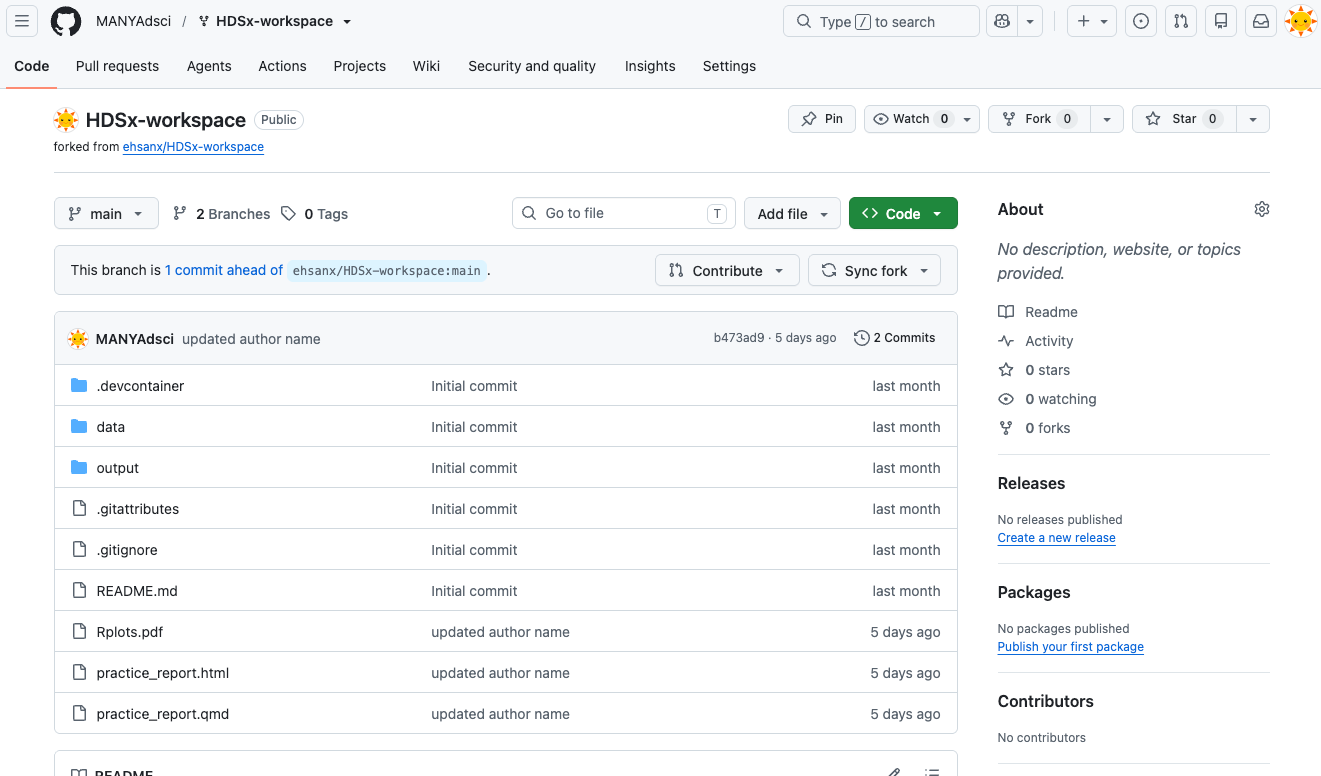
\includegraphics[keepaspectratio]{weeks/week02-modern-workflows/../../assets/images/workflow1/github.png}}

  }

  \caption{The code will be stored and accessible on GitHub as long as
  the company exists. Given that it's owned by a large corporation like
  Microsoft, it will likely last for a long time.}

  \end{figure}%
\item
  Safe if your computer crashes
\item
  This is your \textbf{master copy}
\end{itemize}

\section{Codespace (Public Computer)}\label{codespace-public-computer}

Codespaces is like a library computer:

\begin{itemize}
\item
  \textbf{Temporary machine} It is a disposable environment. If it
  breaks, we just delete it and get a new one.

  \begin{figure}[H]

  {\centering \pandocbounded{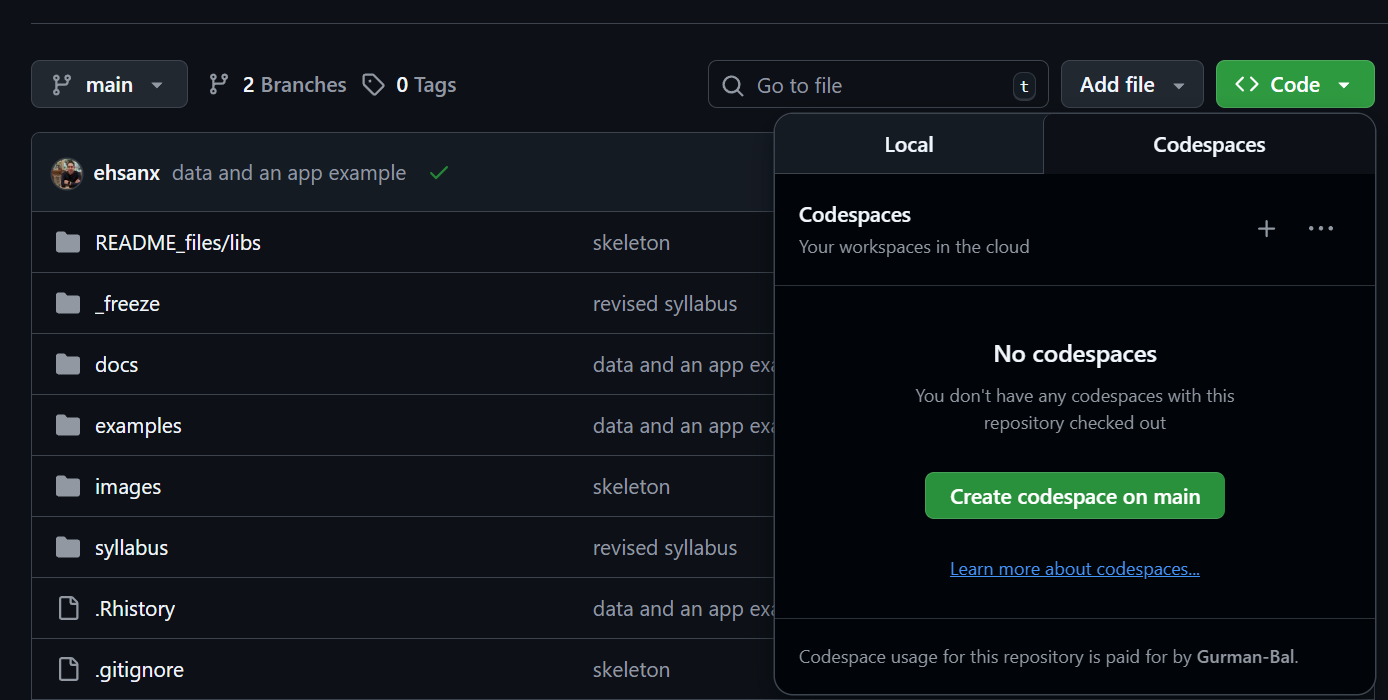
\includegraphics[keepaspectratio]{weeks/week02-modern-workflows/../../assets/images/workflow1/codespace1.png}}

  }

  \caption{Can be accessed by clicking the
  \texttt{\textless{}\textgreater{}\ Code} button, navigating to the
  Codespaces tab, and then starting up a Codespace which contains all
  the file in the Repo.}

  \end{figure}%
\item
  \textbf{Pre-installed software} It comes with R, Python, and Quarto
  installed, so you don't have to install anything on your own laptop.
\item
  \textbf{The ``Two-Save'' Rule (Crucial)} Because this is a temporary
  computer, there are two steps to saving:

  \begin{enumerate}
  \def\labelenumi{\arabic{enumi}.}
  \tightlist
  \item
    \textbf{Ctrl+S (Save):} This only saves to the temporary machine. If
    the machine times out (closes), this is lost.
  \item
    \textbf{Commit \& Push:} This sends your work back to the Repository
    (Cloud Drive). This is the only way to be safe.
  \end{enumerate}
\end{itemize}

\textbf{Warning:} If you close the tab without ``Committing'' (Sending),
your work is erased.

\subsection{Check for understanding}\label{check-for-understanding}

Answer:

\begin{itemize}
\tightlist
\item
  Where are your permanent files stored?
\item
  What happens if you press \texttt{Ctrl+S} but never commit?
\end{itemize}

\chapter{Tour of the Repository}\label{tour-of-the-repository}

\section{Step-by-step}\label{step-by-step}

\begin{enumerate}
\def\labelenumi{\arabic{enumi}.}
\item
  Open your course repository on GitHub\\

  \begin{figure}[H]

  {\centering \pandocbounded{
\includegraphics[keepaspectratio]{weeks/week02-modern-workflows/../../assets/images/workflow2/github.png}}

  }

  \caption{Main github page}

  \end{figure}%
\item
  Click the \textbf{Code} tab\\
  \pandocbounded{\includegraphics[keepaspectratio]{weeks/week02-modern-workflows/../../assets/images/workflow2/code.png}}

  \begin{itemize}
  \tightlist
  \item
    \textbf{Why?} GitHub has many tabs (Issues, Actions, Settings). The
    \textbf{Code} tab is your ``Reset'' button. If you ever get lost in
    a menu, click this to go back to your files.
  \end{itemize}
\item
  Look at the file list\\
  \pandocbounded{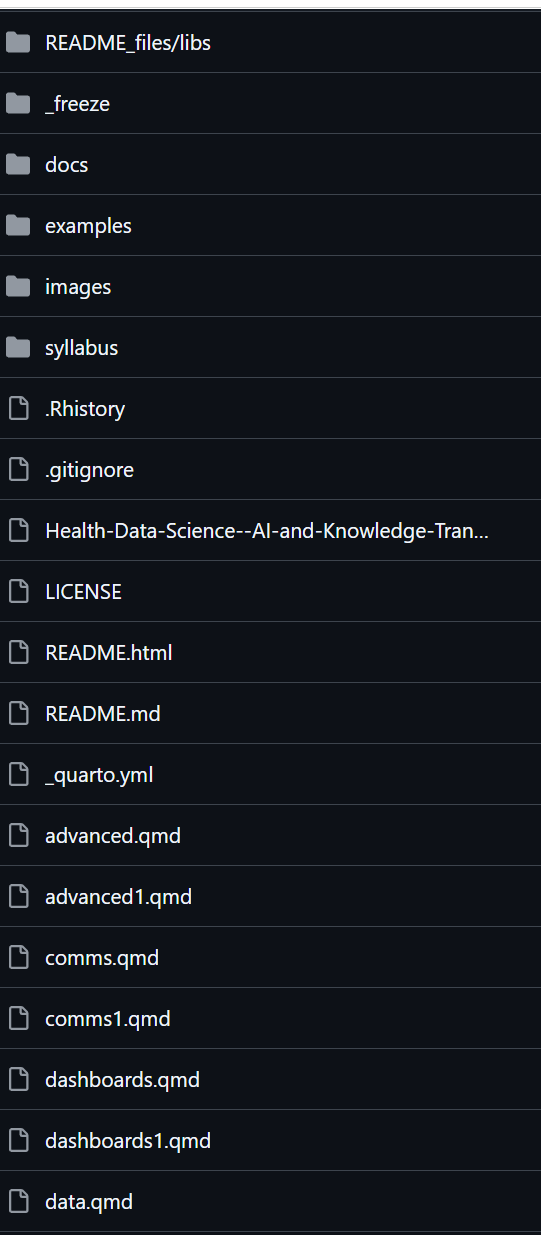
\includegraphics[keepaspectratio]{weeks/week02-modern-workflows/../../assets/images/workflow2/files.png}}

  \begin{itemize}
  \tightlist
  \item
    This shows the \textbf{current state} of the project in the Vault.
  \item
    \textbf{Crucial:} If a file is listed here, it is safe. If it is
    \emph{not} here, it only exists on your temporary ``Desk''
    (Codespace) and is at risk of being lost.
  \end{itemize}
\item
  Scroll to read the README

  \begin{itemize}
  \tightlist
  \item
    The \texttt{README.md} file is displayed automatically at the
    bottom. Think of it as the ``Cover Sheet'' or ``Instruction Manual''
    for your project.
  \end{itemize}
\end{enumerate}

\section{Task}\label{task-1}

Find this file:

\begin{verbatim}
practice_report.qmd
\end{verbatim}

\textbf{Verification:} If you can see \texttt{practice\_report.qmd} in
this list, it means the file is safely stored in the cloud (The Vault).

If you can see it, it is safely stored in the cloud.

\chapter{Opening Your First
Codespace}\label{opening-your-first-codespace}

This process is like walking into the library and turning on a computer.
You are creating a fresh, temporary environment in the cloud.

\section{Steps}\label{steps}

\begin{enumerate}
\def\labelenumi{\arabic{enumi}.}
\item
  Click the green \textbf{Code} button

  \begin{itemize}
  \tightlist
  \item
    This button is usually for downloading files, but we are using it to
    launch a computer.
  \end{itemize}

  \begin{figure}[H]

  {\centering \pandocbounded{\includegraphics[keepaspectratio]{weeks/week02-modern-workflows/../../assets/images/workflow3/code.png}}

  }

  \caption{Code button}

  \end{figure}%
\item
  Click the \textbf{Codespaces} tab

  \begin{itemize}
  \tightlist
  \item
    \textbf{Crucial Choice:} You will see two tabs: ``Local'' and
    ``Codespaces.''
  \item
    \textbf{Local:} Means downloading to your own messy laptop (Hard
    mode).
  \item
    \textbf{Codespaces:} Means using the pre-installed cloud computer
    (Easy mode). Always choose this.
  \end{itemize}

  \begin{figure}[H]

  {\centering \pandocbounded{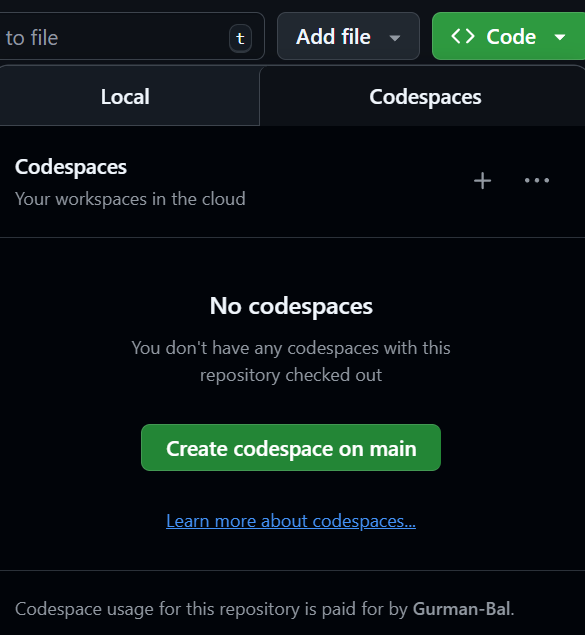
\includegraphics[keepaspectratio]{weeks/week02-modern-workflows/../../assets/images/workflow3/codespaces.png}}

  }

  \caption{Codespaces tab}

  \end{figure}%
\item
  Click \textbf{Create Codespace on main}

  \begin{itemize}
  \tightlist
  \item
    This tells GitHub to build a new computer for you from scratch.
  \end{itemize}

  \begin{figure}[H]

  {\centering \pandocbounded{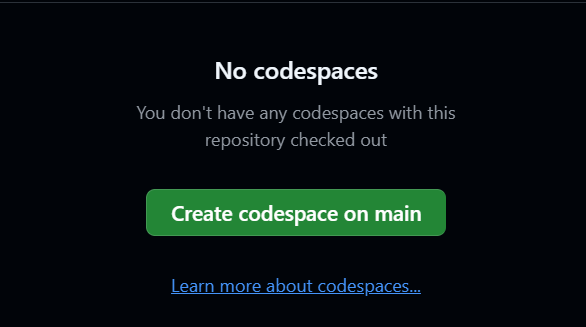
\includegraphics[keepaspectratio]{weeks/week02-modern-workflows/../../assets/images/workflow3/create.png}}

  }

  \caption{Create Codespace}

  \end{figure}%
\end{enumerate}

\section{The ``Boot Up'' Phase}\label{the-boot-up-phase}

\textbf{Wait 2--3 minutes.}

\begin{itemize}
\tightlist
\item
  \textbf{What is happening?} GitHub is silently installing R, Python,
  Quarto, and all the course libraries for you.
\item
  \textbf{The Analogy:} Think of this as the ``ventilation system''
  starting up in a lab. It takes a moment to get the environment ready.
\end{itemize}

\textbf{Success:} You should see \textbf{VS Code} (a dark-themed code
editor) appear in your browser window.

\chapter{Reopening a Codespace}\label{reopening-a-codespace}

\textbf{The Rule:} Do not create a new Codespace each time you log in.

\begin{itemize}
\tightlist
\item
  \textbf{Why?} If you click the green ``Create'' button again, GitHub
  builds a \emph{second} computer.
\item
  \textbf{The Risk:} If you left uncommitted work (Drafts) on ``Computer
  A'' and you start ``Computer B,'' your work will appear lost. It isn't
  lost: it's just on the other computer.
\end{itemize}

To resume exactly where you left off:

\section{Steps}\label{steps-1}

\begin{enumerate}
\def\labelenumi{\arabic{enumi}.}
\item
  Go to the \textbf{Codespace Dashboard}:
  \url{https://github.com/codespaces}

  \begin{itemize}
  \tightlist
  \item
    Think of this as the ``Front Desk'' where all your active computers
    are listed.
  \end{itemize}
\item
  Find your Codespace

  \begin{itemize}
  \tightlist
  \item
    Look for the box labeled with your course repository name.
  \item
    \textbf{Note:} GitHub gives each Codespace a funny random name
    (e.g., \emph{literate-computing-machine} or
    \emph{glorious-couscous}). This is the name of your rented desk.
  \end{itemize}

  \begin{figure}[H]

  {\centering \pandocbounded{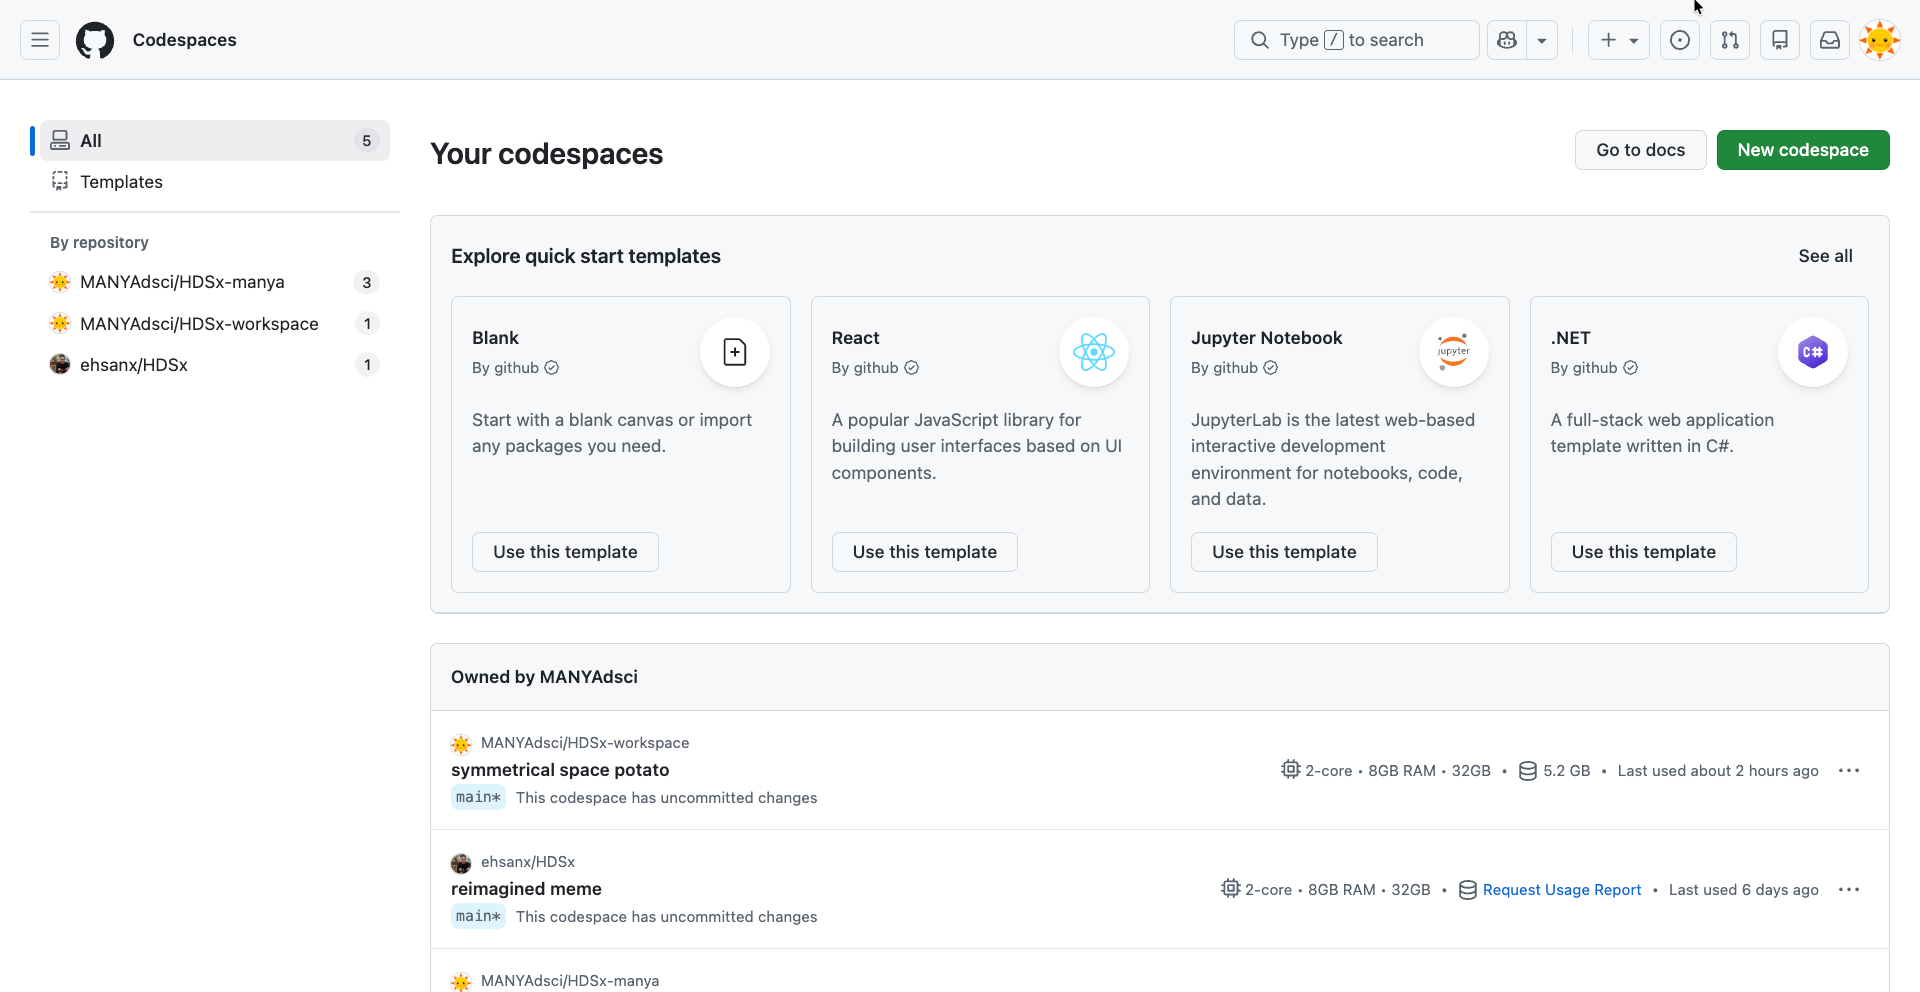
\includegraphics[keepaspectratio]{weeks/week02-modern-workflows/../../assets/images/workflow4/codespace_page.png}}

  }

  \caption{GitHub Codespaces}

  \end{figure}%
\item
  Click the \textbf{Name} of the Codespace

  \begin{itemize}
  \tightlist
  \item
    Do \textbf{not} click the ``New codespace'' button in the corner.
    Click the text link of the funny name.
  \end{itemize}

  \begin{figure}[H]

  {\centering \pandocbounded{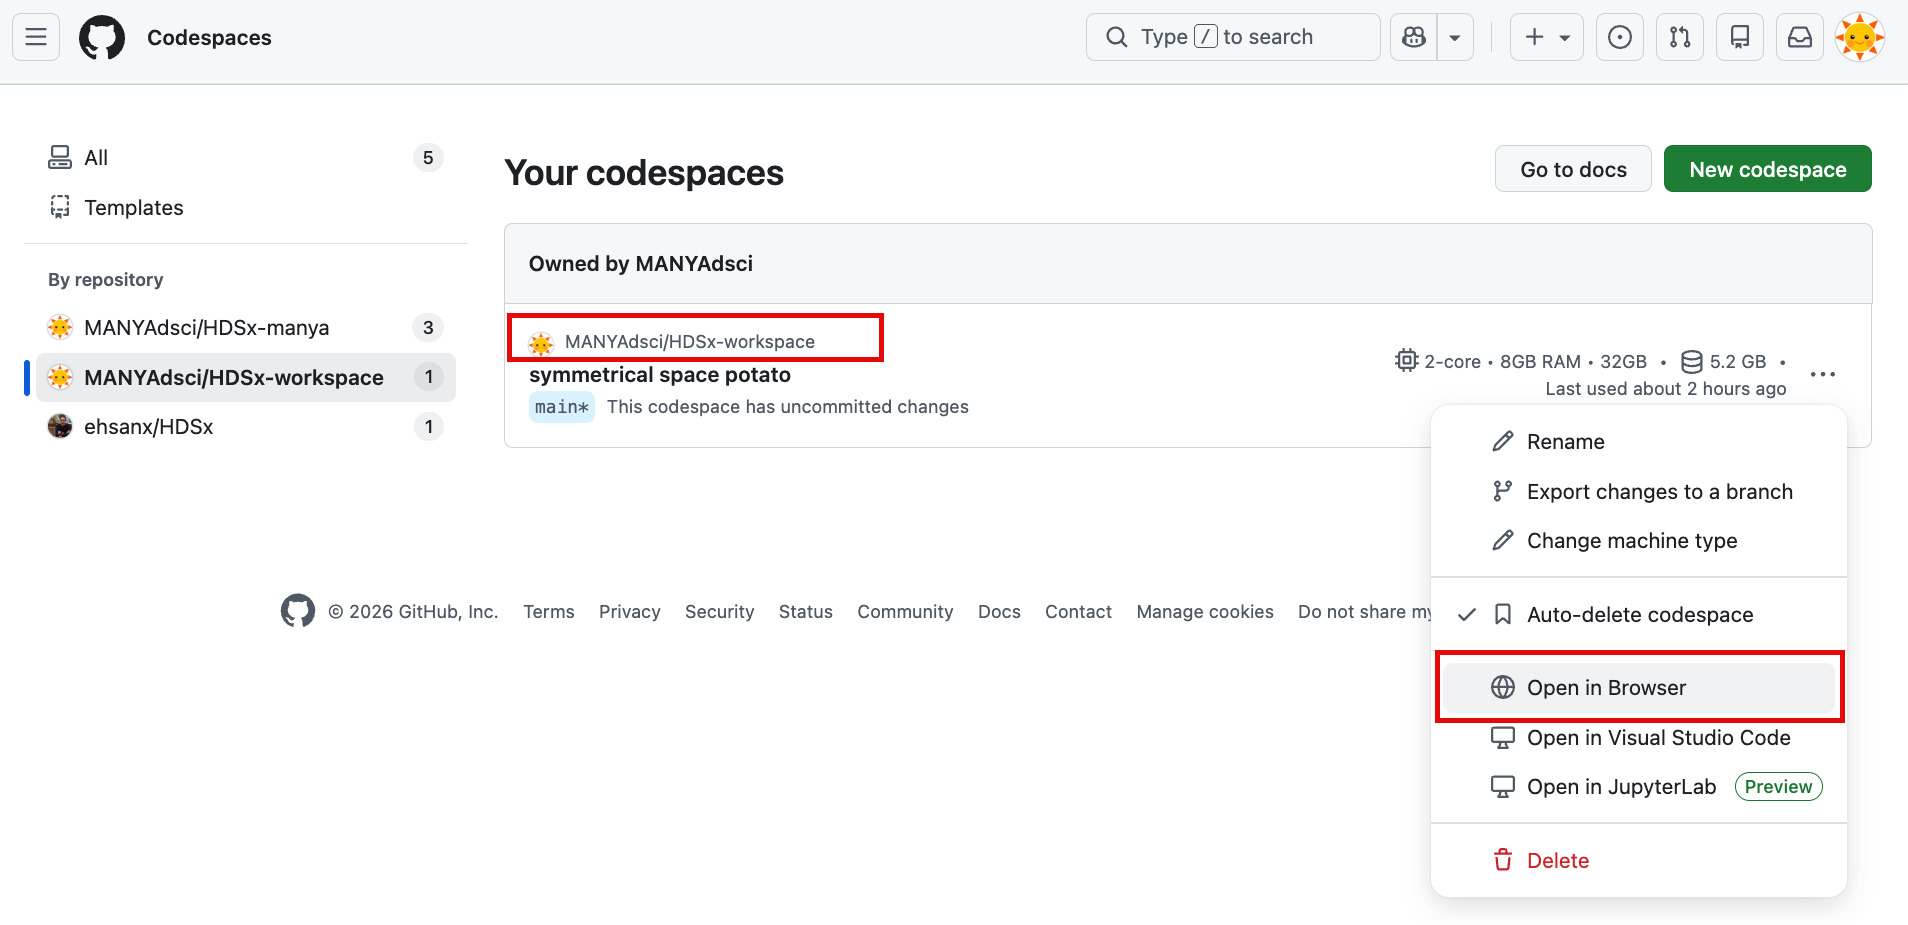
\includegraphics[keepaspectratio]{weeks/week02-modern-workflows/../../assets/images/workflow4/owned.png}}

  }

  \caption{Your Codespace}

  \end{figure}%
\item
  Wait for it to resume

  \begin{itemize}
  \tightlist
  \item
    \textbf{Benefit:} Resuming an existing Codespace is much faster than
    creating a fresh one because the software is already installed.
  \end{itemize}
\end{enumerate}

\chapter{VS Code Orientation}\label{vs-code-orientation}

\pandocbounded{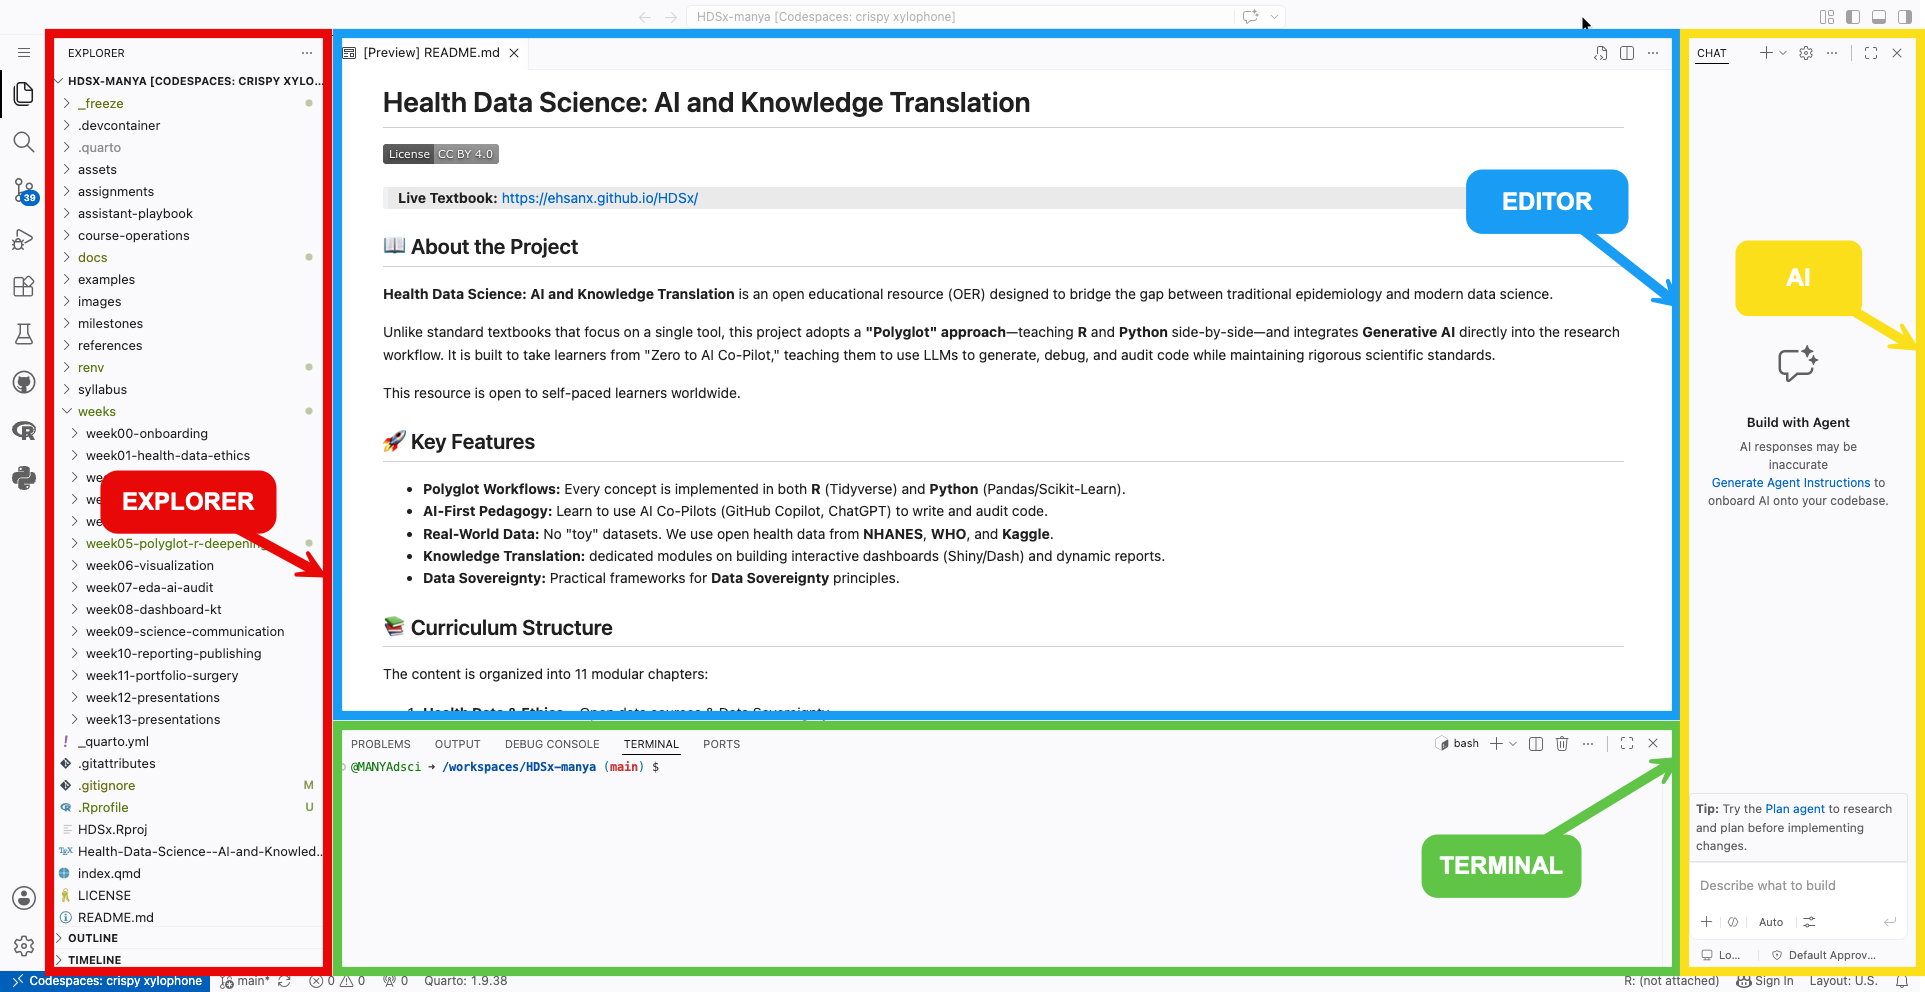
\includegraphics[keepaspectratio]{weeks/week02-modern-workflows/../../assets/images/workflow5/main.png}}

When you open a Codespace, you are using a version of \textbf{VS Code}
in your browser. It has the same interface as the desktop version used
by professional software engineers at Google and Microsoft.

\textbf{Don't Panic:} The interface looks complex because it has
hundreds of features. \textbf{You only need to know three areas.} You
can safely ignore 90\% of the buttons you see.

\section{Explorer (left)}\label{explorer-left}

\textbf{The ``File Cabinet''}

\begin{figure}[H]

{\centering \pandocbounded{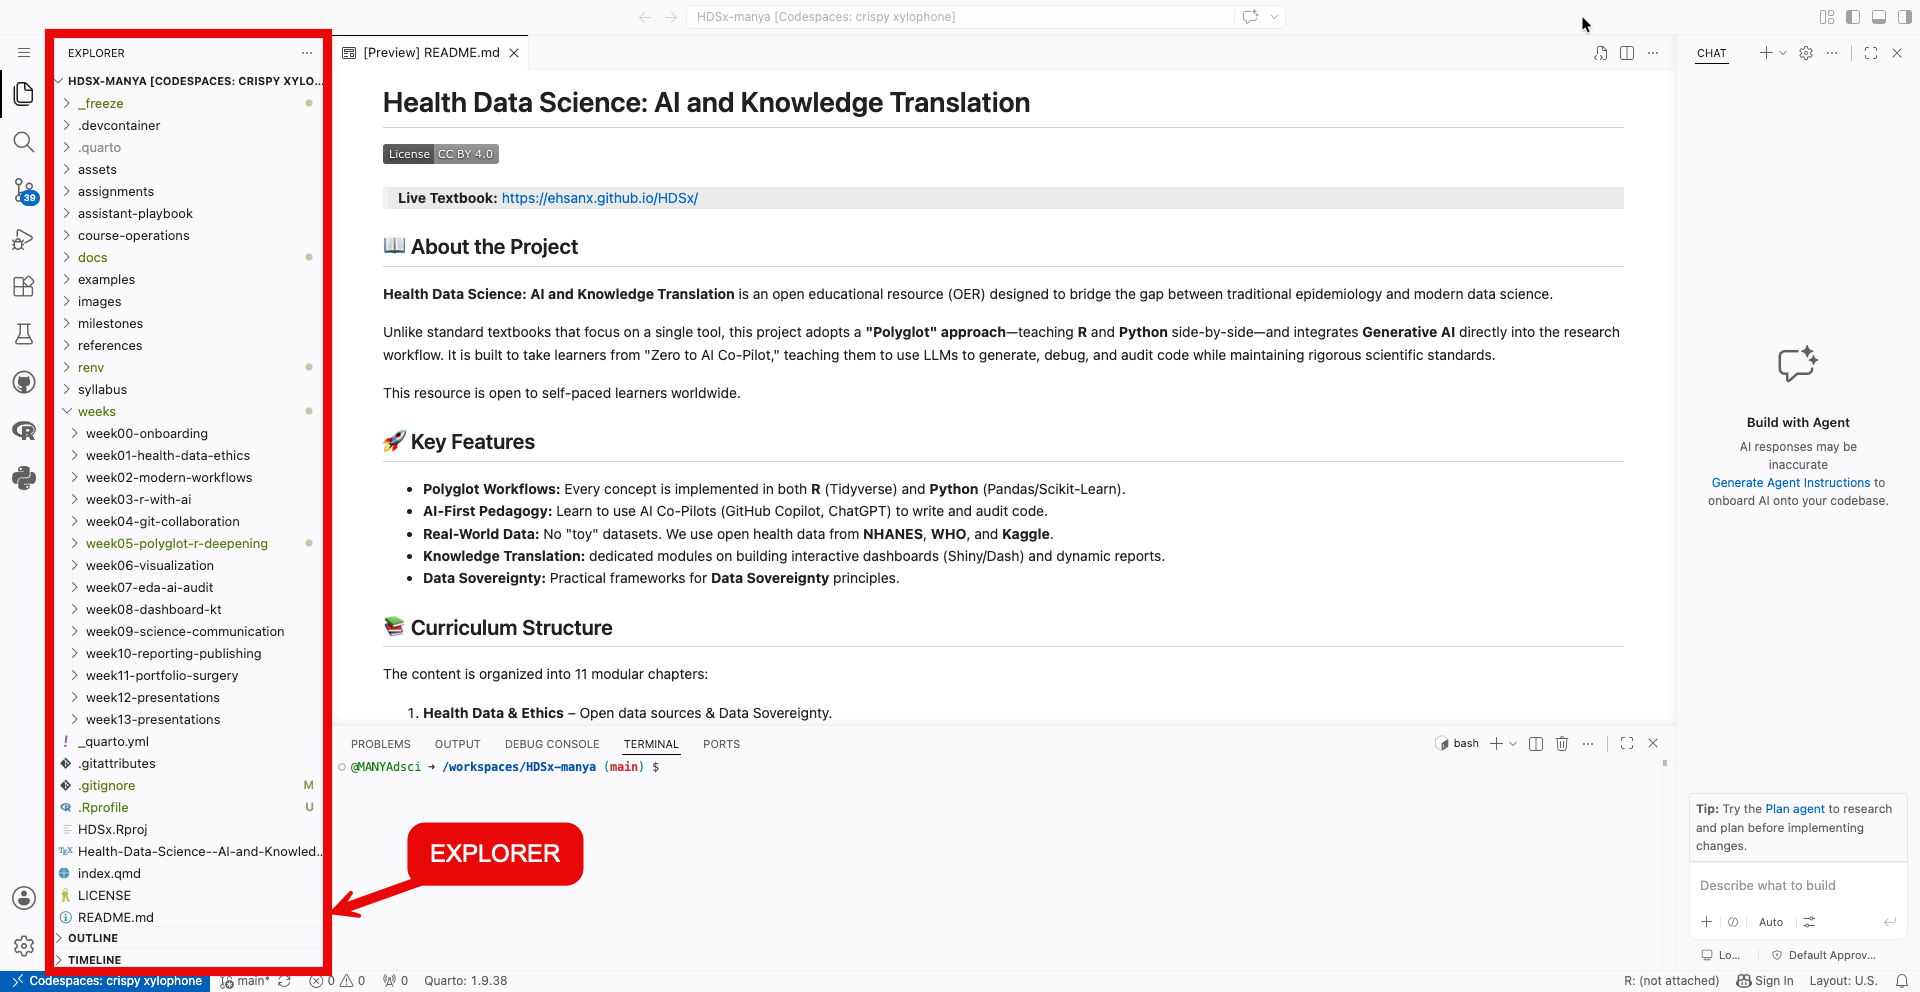
\includegraphics[keepaspectratio]{weeks/week02-modern-workflows/../../assets/images/workflow5/explorer.png}}

}

\caption{Shows files and folders.}

\end{figure}%

\begin{itemize}
\tightlist
\item
  This shows your folders (directories) and files.
\item
  Think of this as your navigation pane. Double-click a file here to
  open it in the Editor.
\end{itemize}

\section{Editor (center)}\label{editor-center}

\textbf{The ``Notebook''}

\begin{figure}[H]

{\centering \pandocbounded{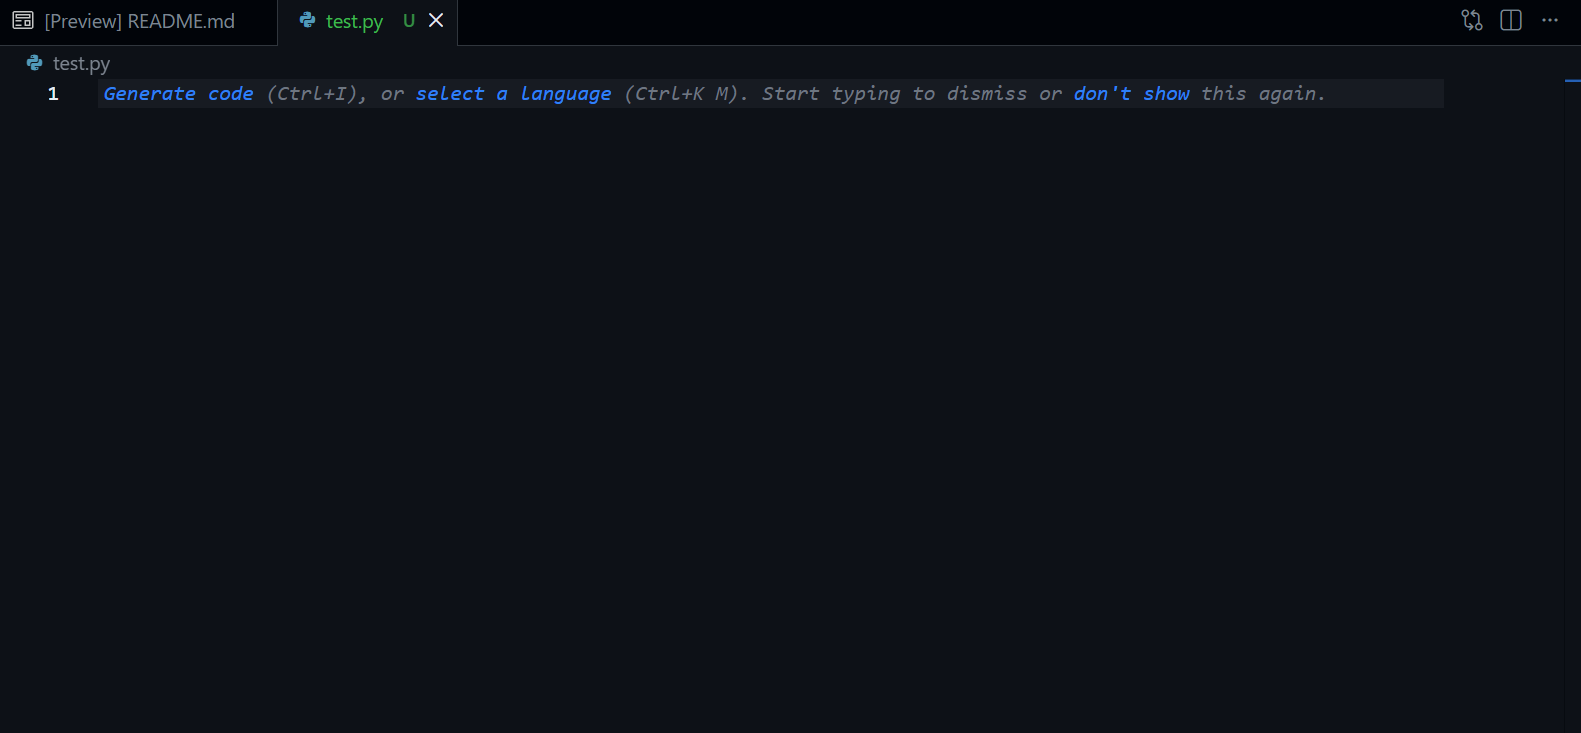
\includegraphics[keepaspectratio]{weeks/week02-modern-workflows/../../assets/images/workflow5/editor.png}}

}

\caption{Where you type.}

\end{figure}%

\begin{itemize}
\tightlist
\item
  This is where you do your actual work: typing code and writing text.
\item
  In this course, you will mostly be editing \texttt{.qmd} (Quarto)
  files here.
\end{itemize}

\section{Terminal (bottom)}\label{terminal-bottom}

\textbf{The ``Engine Room''}

\begin{figure}[H]

{\centering \pandocbounded{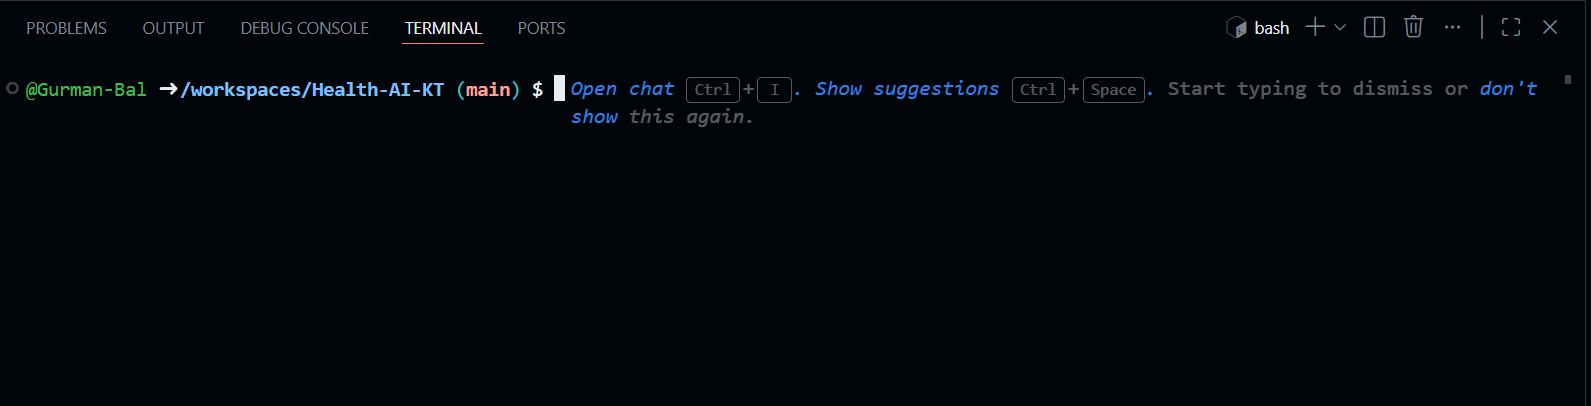
\includegraphics[keepaspectratio]{weeks/week02-modern-workflows/../../assets/images/workflow5/terminal.png}}

}

\caption{Terminal window}

\end{figure}%

\begin{itemize}
\tightlist
\item
  This is where R and Python actually run.
\item
  You will see text scrolling here when you ``Render'' a document. It
  looks like ``The Matrix,'' but it is usually just the computer telling
  you what it is working on.
\end{itemize}

If the terminal disappears (or you accidentally close it):

\textbf{View → Terminal}

\subsection{Mini Task}\label{mini-task}

Open and close a few files in the Explorer to get comfortable with the
layout.

\chapter{Files vs Folders}\label{files-vs-folders}

We use a consistent structure to ensure reproducibility. In Data
Science, being ``organized'' isn't just about being neat---it is a
requirement for your code to work on someone else's machine.

\section{The Golden Rule of Health
Data}\label{the-golden-rule-of-health-data}

We treat data like a \textbf{Crime Scene}---never touch the evidence.

\begin{itemize}
\tightlist
\item
  \textbf{Start:} \texttt{data/} (The Crime Scene). \textbf{READ ONLY.}

  \begin{itemize}
  \tightlist
  \item
    \emph{Rule:} Never open a dataset in Excel and ``fix'' a typo. That
    is tampering with evidence.
  \item
    \emph{Correct Way:} Load the ``dirty'' data into R/Python and fix
    the typo using code. This leaves a trail of exactly what you
    changed.
  \end{itemize}
\item
  \textbf{End:} \texttt{output/} (The Evidence). All graphs and cleaned
  tables go here.
\item
  \textbf{The Detective:} Your code (\texttt{.qmd}) moves information
  from Start to End.
\end{itemize}

\section{Files vs.~Folders (The Mental
Model)}\label{files-vs.-folders-the-mental-model}

\begin{itemize}
\tightlist
\item
  \textbf{Files (e.g., \texttt{report.qmd}):} These are \textbf{sheets
  of paper}. You write on them.
\item
  \textbf{Folders (e.g., \texttt{data/}):} These are \textbf{labeled
  boxes}. You store things in them.
\end{itemize}

\section{Create a folder}\label{create-a-folder}

In Explorer:

\begin{enumerate}
\def\labelenumi{\arabic{enumi}.}
\tightlist
\item
  Right-click anywhere in the blank space of the Explorer pane.
  \pandocbounded{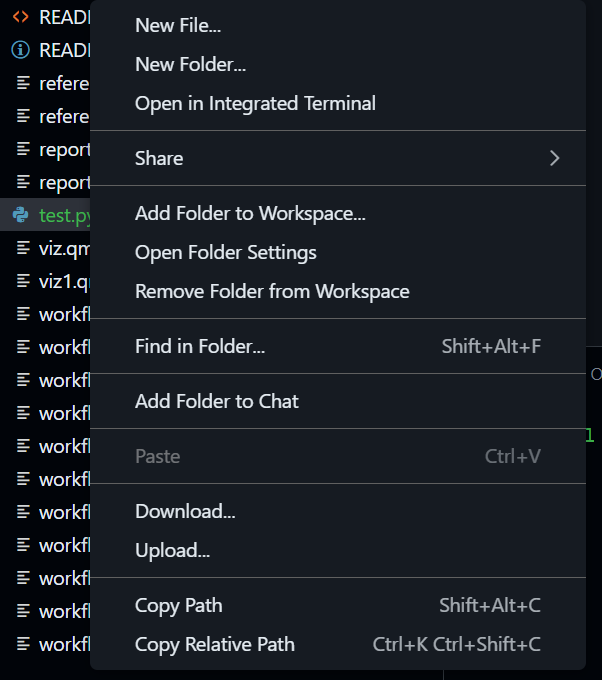
\includegraphics[keepaspectratio]{weeks/week02-modern-workflows/../../assets/images/workflow6/rightclick.png}}
\item
  Select \textbf{New Folder}
\item
  Name it:
\end{enumerate}

\begin{verbatim}
images
\end{verbatim}

\textbf{Pro Tip:} Always use \textbf{lowercase} and \textbf{no spaces}
for folder names (e.g., \texttt{my\_data}, not \texttt{My\ Data}).
Computers struggle with spaces in file paths.

\section{Typical structure}\label{typical-structure}

Your project should always look like this:

\begin{verbatim}
data/      raw data  
output/    generated results  
images/    screenshots  
.qmd       reports  
\end{verbatim}

\textbf{Remember:} The \texttt{data} folder is for \emph{input}. The
\texttt{output} folder is for \emph{results}. They should never mix.

\chapter{The Magic Moment: Render
Quarto}\label{the-magic-moment-render-quarto}

\section{Why do we ``Render''?}\label{why-do-we-render}

In the old days, you would run code, copy a graph, save it as a JPG, and
paste it into Word. If the data changed, you had to redo every step
manually.

\textbf{The Better Way:} Think of your code (\texttt{.qmd} file) as a
\textbf{Recipe} and the final report (HTML/PDF) as the \textbf{Meal}. *
\textbf{Editing:} You don't change the meal; you change the recipe. *
\textbf{Rendering:} This is the ``cooking'' process. When you click
\textbf{Render}, the computer follows your instructions from scratch to
create a fresh meal.

This is the secret to reproducibility: if you give your recipe to a
friend, they can cook the exact same meal.

\section{Step 1 --- Open the file}\label{step-1-open-the-file}

\begin{enumerate}
\def\labelenumi{\arabic{enumi}.}
\tightlist
\item
  Go to the \textbf{Explorer} pane (Left side).
\item
  Locate and click on the file:
\end{enumerate}

\begin{verbatim}
practice_report.qmd
\end{verbatim}

This will open the ``Source Code'' in the center Editor window. You will
see a mix of normal text and code chunks.

\section{Step 2 --- Edit name (The YAML
Header)}\label{step-2-edit-name-the-yaml-header}

Look at the very top of the file. You will see a block of text
sandwiched between three dashes (\texttt{-\/-\/-}). This is called the
\textbf{YAML Header}. It controls the document's metadata.

Find the line that says \texttt{author:}

\begin{verbatim}
author: "Your Name"
\end{verbatim}

\textbf{Task:} Delete ``Your Name'' and type your actual name inside the
quotes. Do not remove the quotes!

\section{Step 3 --- Render}\label{step-3-render}

\begin{enumerate}
\def\labelenumi{\arabic{enumi}.}
\tightlist
\item
  Look for the \textbf{Render} button at the top of the Editor pane (it
  often looks like a Blue Arrow pointing right, or simply says
  ``Render'').
\item
  \textbf{Click it.}
\item
  \textbf{Observe:}

  \begin{itemize}
  \tightlist
  \item
    \textbf{The Terminal (Bottom):} You will see text scrolling quickly.
    This is R/Python executing your code chunks.
  \item
    \textbf{The Preview (Right):} A new window should appear showing a
    beautiful, formatted report with your name on it.
  \end{itemize}
\end{enumerate}

\textbf{Congratulations!} You just performed ``Knowledge
Translation''---turning raw code into a human-readable document.

\section{If it fails
(Troubleshooting)}\label{if-it-fails-troubleshooting}

Rendering involves many moving parts, so it sometimes gets stuck.

\begin{itemize}
\tightlist
\item
  \textbf{The ``Wait'' Rule:} If nothing happens for 20 seconds, the
  background process might be initializing. Give it a moment.
\item
  \textbf{The ``Retry'' Rule:} Sometimes the connection hiccups. Click
  \textbf{Render} one more time.
\item
  \textbf{The ``Red Text'' Rule:} Look at the \textbf{Terminal} tab at
  the bottom. If you see red text, it is an error message. Read it---it
  usually tells you exactly what went wrong (e.g., ``File not found'' or
  ``Syntax error'').
\end{itemize}

\chapter{Commit Your Work}\label{commit-your-work}

Your work is currently only on the ``Rented Desk'' (Codespace). It is a
\textbf{Draft}. To save it permanently to the ``Vault'' (GitHub), you
must \textbf{Commit} and \textbf{Push} (Send).

\textbf{The Analogy:} Think of this like shipping a package. You have
packed the box (saved the file), but now you need to put a label on it
and hand it to the courier.

\section{Steps}\label{steps-2}

\begin{enumerate}
\def\labelenumi{\arabic{enumi}.}
\item
  Click the \textbf{Source Control} icon

  \begin{itemize}
  \tightlist
  \item
    It looks like a \textbf{blue bubble} or a \textbf{connect-the-dots
    graph} on the far left sidebar.
  \item
    This opens the ``Shipping Department.'' You will see a list of every
    file you changed.
  \end{itemize}

  \begin{figure}[H]

  {\centering \pandocbounded{
\includegraphics[keepaspectratio]{weeks/week02-modern-workflows/../../assets/images/workflow8/button.png}}

  }

  \caption{Source control icon circled in red}

  \end{figure}%
\item
  Type a \textbf{Commit Message}

  \begin{itemize}
  \tightlist
  \item
    \textbf{The Label:} You cannot ship a package without a label.
  \item
    \textbf{What to write:} Be descriptive but brief. Imagine you are
    leaving a note for your future self about \emph{what} you did.
  \item
    \emph{Example:} ``Updated author name in practice report''.
  \item
    \emph{Bad Example:} ``stuff'' or ``fix''.
  \end{itemize}

  \begin{figure}[H]

  {\centering \pandocbounded{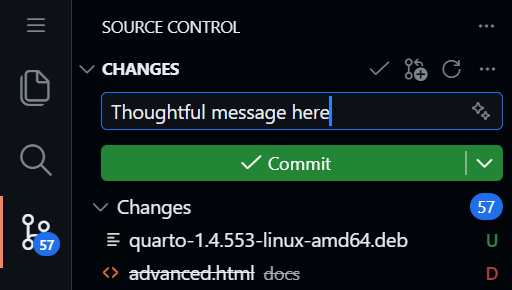
\includegraphics[keepaspectratio]{weeks/week02-modern-workflows/../../assets/images/workflow8/message.png}}

  }

  \caption{This is required}

  \end{figure}%
\item
  Click \textbf{Commit and Sync} (or Commit and Push)

  \begin{itemize}
  \tightlist
  \item
    This is the \textbf{``Send''} button.
  \item
    \textbf{Action:} It wraps up your changes, stamps them with the time
    and your message, and teleports them to the Cloud Vault.
  \item
    \emph{Note:} You might be asked to click ``Always'' or ``Yes'' to
    confirm the sync.
  \end{itemize}

  \begin{figure}[H]

  {\centering \pandocbounded{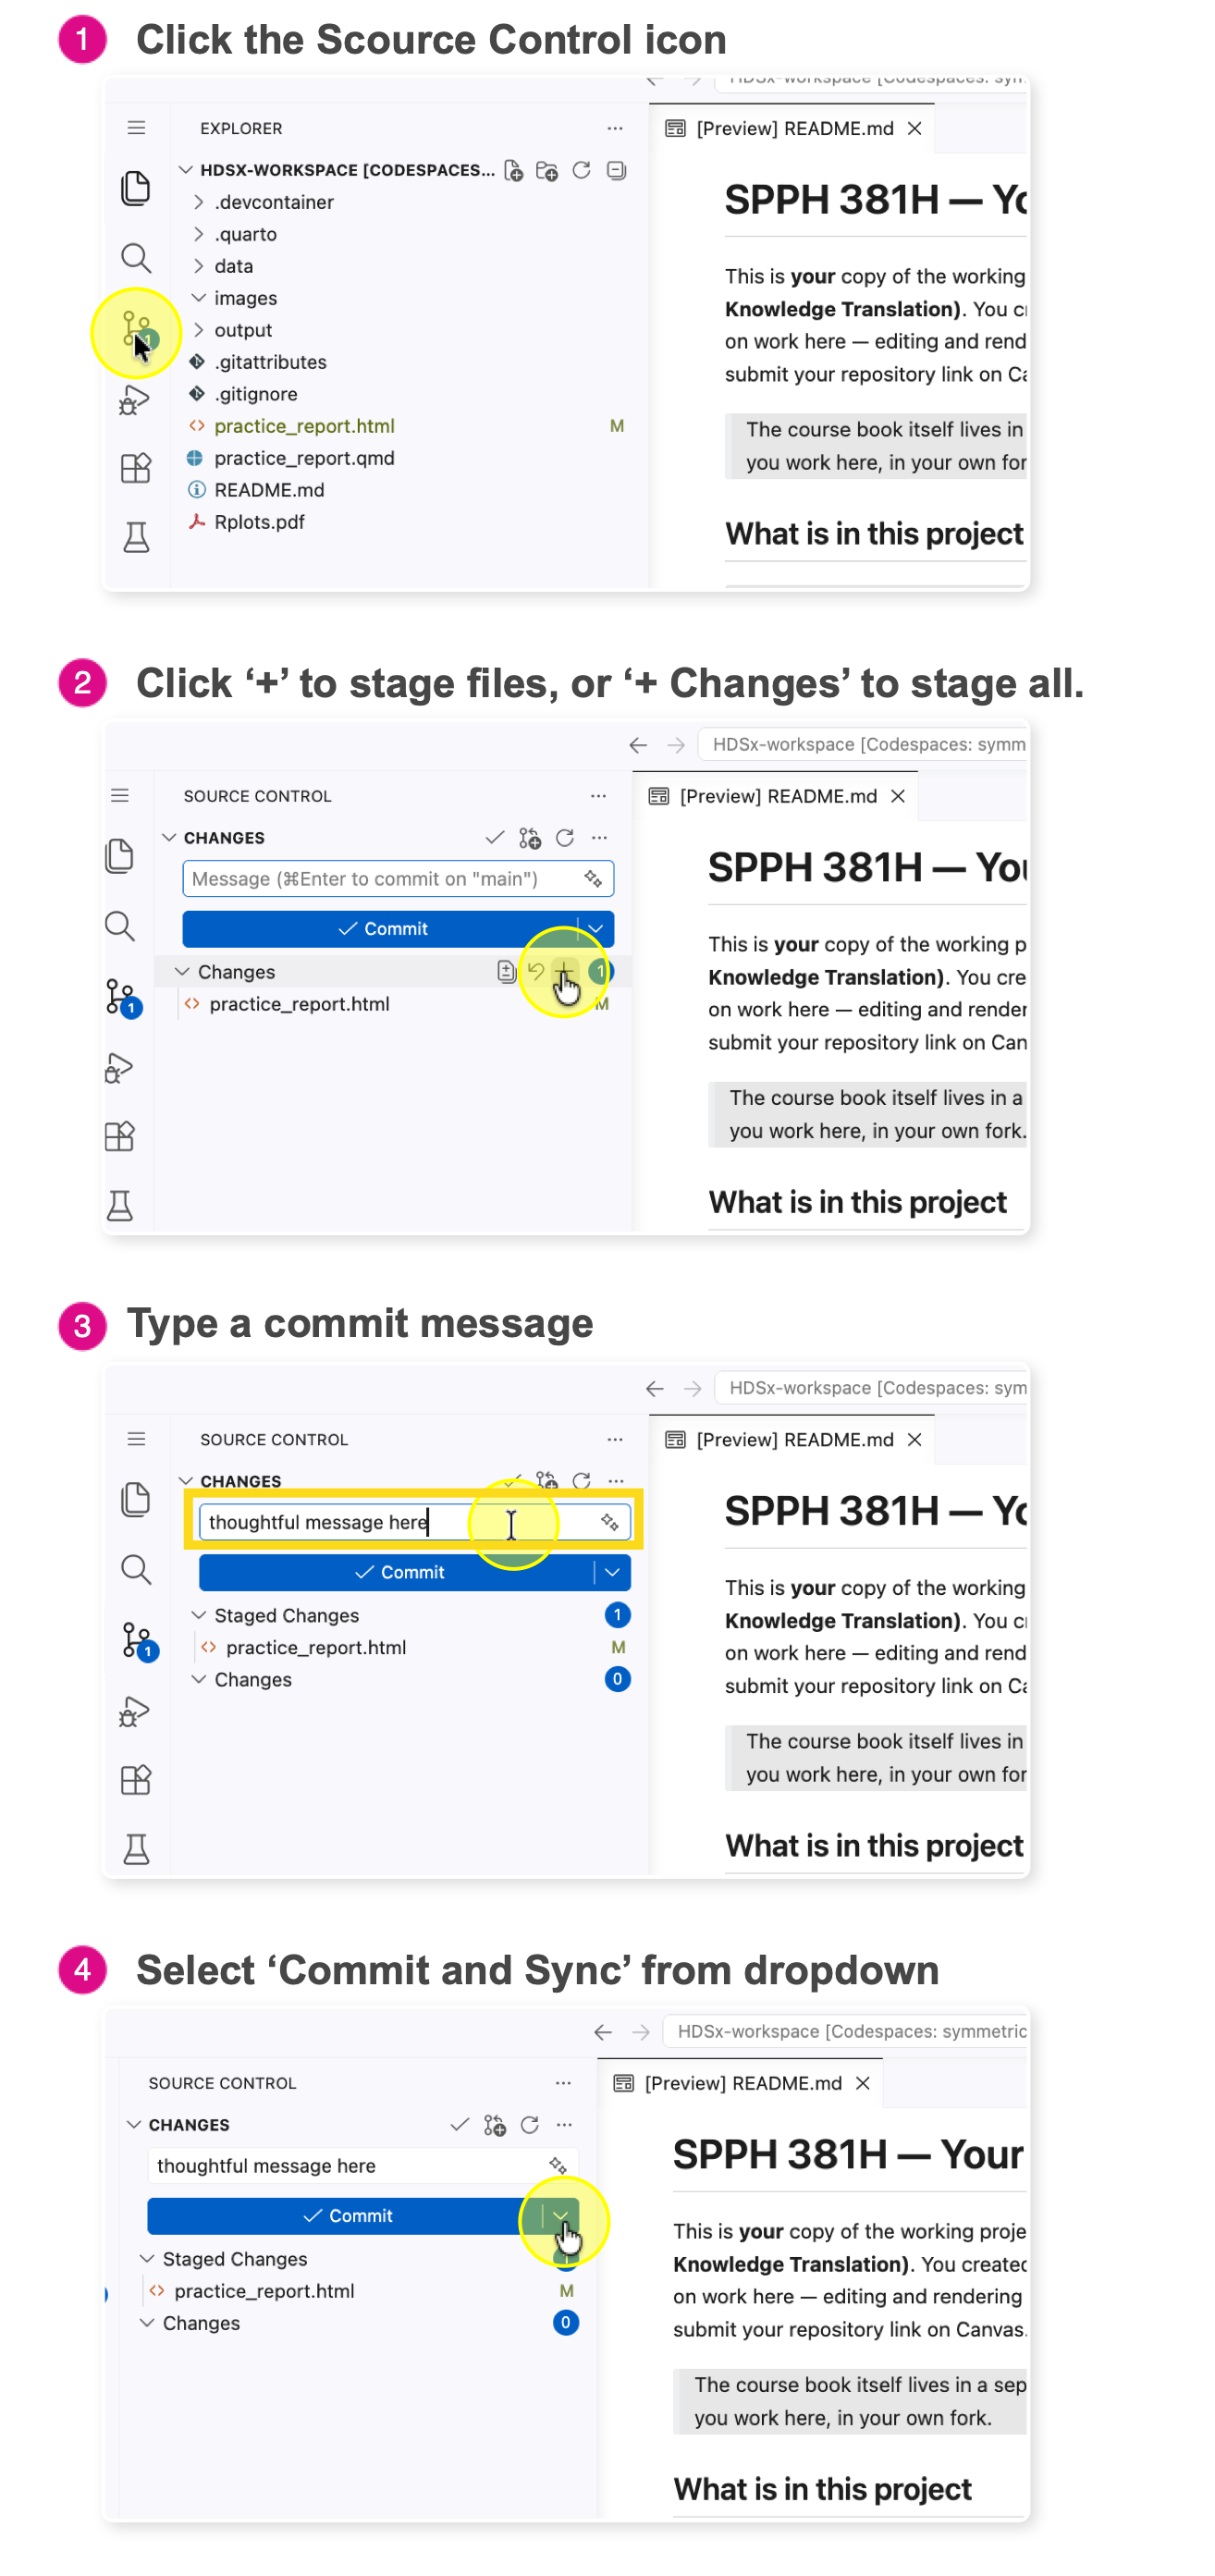
\includegraphics[keepaspectratio]{weeks/week02-modern-workflows/../../assets/images/workflow8/commitpush.png}}

  }

  \caption{This will push your changes to the remote branch}

  \end{figure}%
\end{enumerate}

\section{Verify (Trust but Verify)}\label{verify-trust-but-verify}

Did it actually work?

\begin{enumerate}
\def\labelenumi{\arabic{enumi}.}
\tightlist
\item
  Go back to your \textbf{GitHub Repository} tab (The Vault).
\item
  \textbf{Refresh} the page.
\item
  Look at the file list. You should see your ``Commit Message''
  displayed next to the file you just edited.
\end{enumerate}

\chapter{Troubleshooting: Rebuild
Container}\label{troubleshooting-rebuild-container}

Sometimes the cloud computer gets ``stuck.'' Maybe the terminal froze,
or R crashed.

\textbf{The Fix:} We don't fix broken computers; we get new ones.
``Rebuilding the Container'' is the cloud equivalent of \textbf{``Have
you tried turning it off and on again?''}---but better, because it gives
you a fresh machine while keeping your files safe.

\section{When to use this?}\label{when-to-use-this}

If things break:

\begin{itemize}
\tightlist
\item
  \textbf{Terminal frozen:} You type, but nothing appears.
\item
  \textbf{Render fails:} You get weird errors that make no sense.
\item
  \textbf{Environment issues:} R or Python can't find a package that was
  there yesterday.
\end{itemize}

\section{Steps}\label{steps-3}

\begin{enumerate}
\def\labelenumi{\arabic{enumi}.}
\tightlist
\item
  \textbf{Open the Command Palette}

  \begin{itemize}
  \tightlist
  \item
    Press \texttt{F1} (or \texttt{Ctrl+Shift+P} on Windows /
    \texttt{Cmd+Shift+P} on Mac).
  \item
    A search bar will appear at the very top of the screen. This is the
    ``God Mode'' search bar for VS Code.
  \end{itemize}
\item
  \textbf{Search}

  \begin{itemize}
  \tightlist
  \item
    Type: \texttt{Rebuild\ Container}
  \end{itemize}
\item
  \textbf{Execute}

  \begin{itemize}
  \tightlist
  \item
    Click on the option that says: \textbf{Codespaces: Rebuild
    Container}
  \end{itemize}
\item
  \textbf{Wait (\textasciitilde2-5 minutes)}

  \begin{itemize}
  \tightlist
  \item
    The screen will reload.
  \item
    \textbf{Don't Panic:} You might see a black screen with scrolling
    text logs. This is normal: it is reinstalling the software.
  \item
    When your files reappear in the Explorer, you are ready to go.
  \end{itemize}
\end{enumerate}

\textbf{Did I lose my work?}

\begin{itemize}
\item
  \textbf{Saved files:} No.~Anything you pressed \texttt{Ctrl+S} on is
  safe.
\item
  \textbf{Unsaved typing:} Yes.
\item
  \textbf{R Memory:} Yes. You will need to re-run your code chunks from
  the top.
\end{itemize}

\chapter{Stop Your Codespace}\label{stop-your-codespace}

Codespaces is not free forever. You have a monthly allowance (approx. 60
hours/month for free accounts).

\textbf{The Analogy:} Think of a Codespace like a \textbf{Taxi}.

\begin{itemize}
\tightlist
\item
  \textbf{Working:} When you are coding, the meter is running.
\item
  \textbf{The Trap:} If you just close your browser tab, it is like
  getting out of the taxi but asking the driver to ``wait here.''
  \textbf{The meter keeps running.}
\item
  \textbf{The Fix:} You must explicitly ``end the ride'' (Stop the
  Codespace).
\end{itemize}

\section{Correct shutdown}\label{correct-shutdown}

\begin{enumerate}
\def\labelenumi{\arabic{enumi}.}
\tightlist
\item
  Go to the \textbf{Codespace Dashboard}:
  \url{https://github.com/codespaces}

  \begin{itemize}
  \tightlist
  \item
    This is your command center.
  \end{itemize}
\item
  Find your active Codespace

  \begin{itemize}
  \tightlist
  \item
    Look for the green text that says ``Active''.
  \end{itemize}
\item
  Click \texttt{...} (The ``Meatball'' Menu)

  \begin{itemize}
  \tightlist
  \item
    It is located on the far right side of the Codespace box.
  \end{itemize}
\item
  Click \textbf{Stop Codespace}

  \begin{itemize}
  \tightlist
  \item
    \textbf{Stop:} This ``pauses'' the computer. It saves your installed
    packages and RAM state so you can resume quickly next time.
    \textbf{(Recommended)}
  \item
    \textbf{Delete:} This destroys the computer. You will have to wait
    2-3 minutes for the ``Boot Up'' phase next time you start.
  \end{itemize}
\end{enumerate}

\textbf{Critical Warning:} Closing the browser tab is \textbf{NOT}
enough.

\begin{itemize}
\item
  GitHub keeps the machine running for \textbf{30 minutes} after you
  close the tab (in case your internet flickered).
\item
  \textbf{The Cost:} If you just close the tab every day, you will waste
  \textasciitilde15 hours of your monthly quota on empty time.
\end{itemize}

\pandocbounded{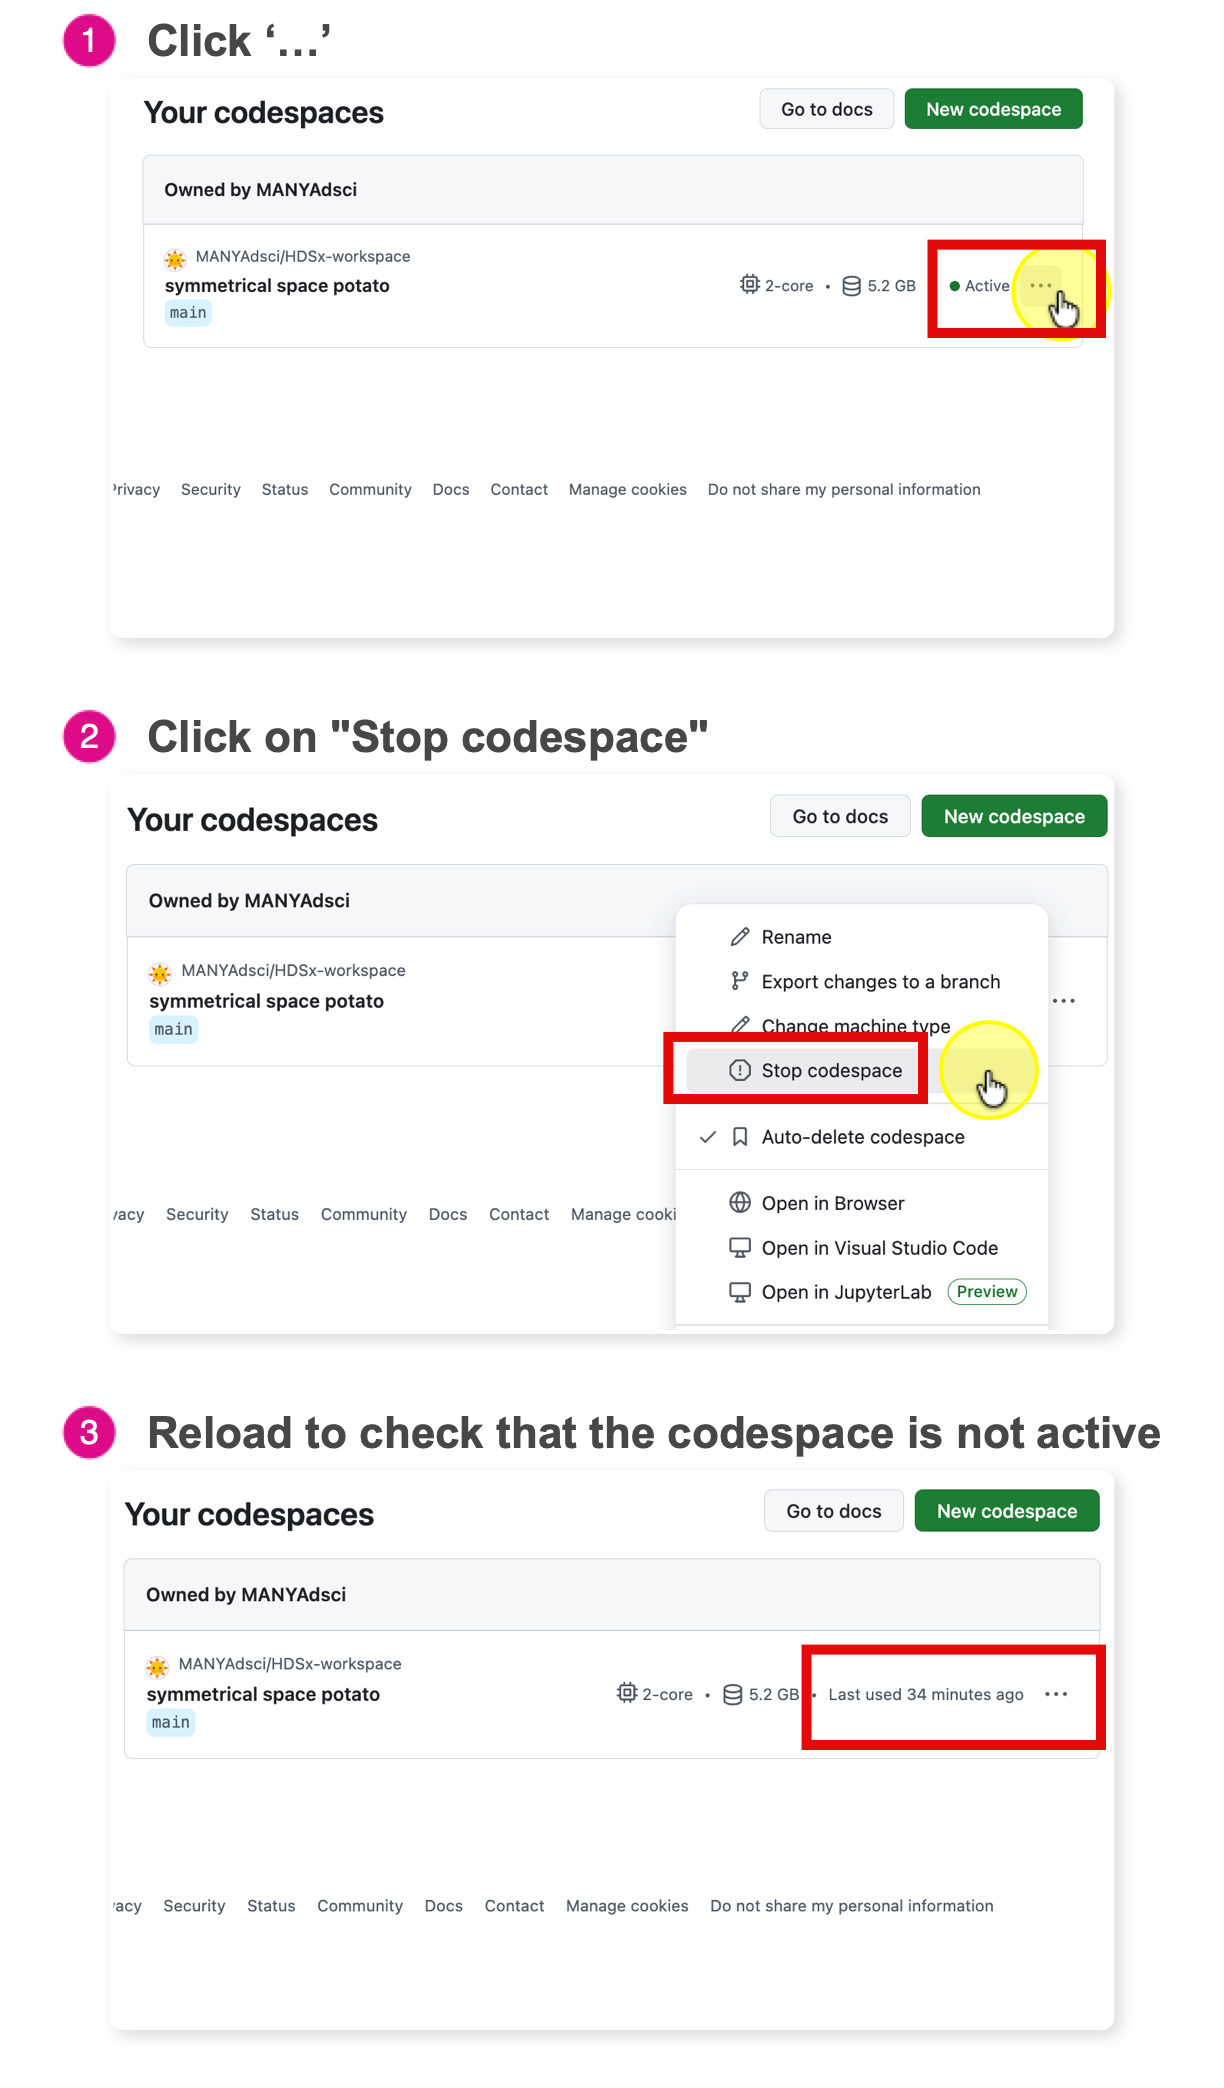
\includegraphics[keepaspectratio]{weeks/week02-modern-workflows/../../assets/images/workflow10/stop.png}}

\chapter{Final Checklist}\label{final-checklist}

\begin{itemize}
\tightlist
\item[$\square$]
  I understand repository vs Codespace\\
\item[$\square$]
  I rendered a \texttt{.qmd} file\\
\item[$\square$]
  I committed changes\\
\item[$\square$]
  I know how to rebuild container\\
\item[$\square$]
  I know how to stop Codespace
\end{itemize}

\section{Reflection}\label{reflection}

Write 2--3 sentences:

\begin{itemize}
\tightlist
\item
  What was easiest?
\item
  What was confusing?
\item
  What questions do you still have?
\end{itemize}

\part{Week 3: R with AI}

\chapter*{Week 3: R with AI}\label{week-3-r-with-ai-1}
\addcontentsline{toc}{chapter}{Week 3: R with AI}

\markboth{Week 3: R with AI}{Week 3: R with AI}

\section*{Overview}\label{overview-2}
\addcontentsline{toc}{section}{Overview}

\markright{Overview}

\textbf{Summary:} In Week 2 you learned how to use your Codespace, edit
a Quarto document, and make your first commit. Now you learn how to
speak R---not by memorizing syntax, but by directing an AI co-pilot and
\emph{auditing} what it writes. Your job is to be the pilot: you decide
what the analysis should do, the AI drafts the code, and you verify
every line before it flies.

\textbf{Learning Objectives:}

\begin{itemize}
\tightlist
\item
  Understand that R is a calculator that needs specific, case-sensitive
  instructions.
\item
  Load packages with \texttt{library()} and explain why this is needed
  each session.
\item
  Use core constructs: variables (assignment), functions (with
  arguments), and the pipe (\texttt{\%\textgreater{}\%} /
  \texttt{\textbar{}\textgreater{}}).
\item
  Perform basic data transformations using \texttt{dplyr} verbs:
  \texttt{filter()}, \texttt{select()}, \texttt{mutate()},
  \texttt{summarise()}, \texttt{group\_by()}.
\item
  Inspect a dataset on first contact: structure, dimensions,
  missingness.
\item
  Identify control flow (\texttt{if/else}, loops) in AI-generated code
  and audit whether it is correct.
\item
  Write and adapt a simple custom function.
\item
  Apply an AI safety checklist to catch hallucinations, wrong column
  names, and unsafe operations.
\item
  Document your analysis in Quarto by weaving code chunks with Markdown
  narrative.
\item
  Commit incrementally as you work (reinforcing Week 2 Git basics).
\end{itemize}

\begin{center}\rule{0.5\linewidth}{0.5pt}\end{center}

\section*{\texorpdfstring{\texttt{r1.qmd} Packages: Opening the
Toolbox}{r1.qmd Packages: Opening the Toolbox}}\label{r1.qmd-packages-opening-the-toolbox}
\addcontentsline{toc}{section}{\texttt{r1.qmd} Packages: Opening the
Toolbox}

\markright{\texttt{r1.qmd} Packages: Opening the Toolbox}

\subsection*{Install vs Load}\label{install-vs-load}
\addcontentsline{toc}{subsection}{Install vs Load}

\begin{itemize}
\tightlist
\item
  \texttt{install.packages("tidyverse")} --- \textbf{buying} the
  toolbox. Done once per environment (already done in your course
  Codespace).
\item
  \texttt{library(tidyverse)} --- \textbf{opening} the toolbox. Required
  every time you restart R or reopen your Codespace.
\end{itemize}

\begin{Shaded}
\begin{Highlighting}[numbers=left,,]
\FunctionTok{library}\NormalTok{(tidyverse)}
\end{Highlighting}
\end{Shaded}

\begin{tcolorbox}[enhanced jigsaw, colframe=quarto-callout-note-color-frame, toptitle=1mm, colback=white, leftrule=.75mm, toprule=.15mm, colbacktitle=quarto-callout-note-color!10!white, breakable, bottomrule=.15mm, opacityback=0, title=\textcolor{quarto-callout-note-color}{\faInfo}\hspace{0.5em}{Note}, rightrule=.15mm, bottomtitle=1mm, opacitybacktitle=0.6, titlerule=0mm, arc=.35mm, left=2mm, coltitle=black]

If you see an error like
\texttt{there\ is\ no\ package\ called\ \textquotesingle{}tidyverse\textquotesingle{}},
the package is not installed in your Codespace. Ask your TA --- this
should be pre-configured.

\end{tcolorbox}

\begin{center}\rule{0.5\linewidth}{0.5pt}\end{center}

\section*{\texorpdfstring{\texttt{r2.qmd} Core Constructs: Boxes,
Toasters, and the Assembly
Line}{r2.qmd Core Constructs: Boxes, Toasters, and the Assembly Line}}\label{r2.qmd-core-constructs-boxes-toasters-and-the-assembly-line}
\addcontentsline{toc}{section}{\texttt{r2.qmd} Core Constructs: Boxes,
Toasters, and the Assembly Line}

\markright{\texttt{r2.qmd} Core Constructs: Boxes, Toasters, and the
Assembly Line}

\subsection*{Variables: The Labeled
Box}\label{variables-the-labeled-box}
\addcontentsline{toc}{subsection}{Variables: The Labeled Box}

R has no memory unless you store results in a named box using
\texttt{\textless{}-}.

\begin{Shaded}
\begin{Highlighting}[numbers=left,,]
\NormalTok{patient\_age }\OtherTok{\textless{}{-}} \DecValTok{55}
\NormalTok{clinic\_name }\OtherTok{\textless{}{-}} \StringTok{"Vancouver General"}
\end{Highlighting}
\end{Shaded}

\begin{tcolorbox}[enhanced jigsaw, colframe=quarto-callout-warning-color-frame, toptitle=1mm, colback=white, leftrule=.75mm, toprule=.15mm, colbacktitle=quarto-callout-warning-color!10!white, breakable, bottomrule=.15mm, opacityback=0, title=\textcolor{quarto-callout-warning-color}{\faExclamationTriangle}\hspace{0.5em}{Warning}, rightrule=.15mm, bottomtitle=1mm, opacitybacktitle=0.6, titlerule=0mm, arc=.35mm, left=2mm, coltitle=black]

\textbf{Case sensitivity:} \texttt{Age}, \texttt{age}, and \texttt{AGE}
are three different boxes. This is one of the most common bugs in
AI-generated code. Always check that column names match your data
exactly.

\end{tcolorbox}

\subsection*{Functions: The Toaster}\label{functions-the-toaster}
\addcontentsline{toc}{subsection}{Functions: The Toaster}

A function takes \textbf{input} and returns \textbf{output}. Arguments
(inside the parentheses) control its behaviour.

\begin{Shaded}
\begin{Highlighting}[numbers=left,,]
\FunctionTok{mean}\NormalTok{(}\FunctionTok{c}\NormalTok{(}\DecValTok{72}\NormalTok{, }\DecValTok{85}\NormalTok{, }\DecValTok{90}\NormalTok{), }\AttributeTok{na.rm =} \ConstantTok{TRUE}\NormalTok{)}
\end{Highlighting}
\end{Shaded}

\begin{itemize}
\tightlist
\item
  \texttt{c(72,\ 85,\ 90)} is the input (a vector of numbers).
\item
  \texttt{na.rm\ =\ TRUE} tells R to ignore missing values.
  \textbf{Always look for this} when auditing AI code that works with
  health data --- missingness is the norm, not the exception.
\end{itemize}

\subsection*{The Pipe: The Assembly
Line}\label{the-pipe-the-assembly-line}
\addcontentsline{toc}{subsection}{The Pipe: The Assembly Line}

The pipe passes the result of one step into the next. Think of it as
\textbf{``and then\ldots{}''}

\begin{Shaded}
\begin{Highlighting}[numbers=left,,]
\NormalTok{data }\SpecialCharTok{\%\textgreater{}\%}
  \FunctionTok{filter}\NormalTok{(age }\SpecialCharTok{\textgreater{}} \DecValTok{65}\NormalTok{) }\SpecialCharTok{\%\textgreater{}\%}
  \FunctionTok{summarise}\NormalTok{(}\AttributeTok{mean\_bmi =} \FunctionTok{mean}\NormalTok{(bmi, }\AttributeTok{na.rm =} \ConstantTok{TRUE}\NormalTok{))}
\end{Highlighting}
\end{Shaded}

Read this as: \emph{``Take the data, and then keep only patients over
65, and then calculate the average BMI.''}

\begin{tcolorbox}[enhanced jigsaw, colframe=quarto-callout-tip-color-frame, toptitle=1mm, colback=white, leftrule=.75mm, toprule=.15mm, colbacktitle=quarto-callout-tip-color!10!white, breakable, bottomrule=.15mm, opacityback=0, title=\textcolor{quarto-callout-tip-color}{\faLightbulb}\hspace{0.5em}{Tip}, rightrule=.15mm, bottomtitle=1mm, opacitybacktitle=0.6, titlerule=0mm, arc=.35mm, left=2mm, coltitle=black]

You will see two pipe symbols in the wild: \texttt{\%\textgreater{}\%}
(from the \texttt{magrittr} / \texttt{tidyverse} packages) and
\texttt{\textbar{}\textgreater{}} (built into R 4.1+). They do the same
thing for our purposes. If AI generates the other one, don't panic ---
both work in your Codespace.

\end{tcolorbox}

\begin{center}\rule{0.5\linewidth}{0.5pt}\end{center}

\section*{\texorpdfstring{\texttt{r3.qmd} Data Import and First
Contact}{r3.qmd Data Import and First Contact}}\label{r3.qmd-data-import-and-first-contact}
\addcontentsline{toc}{section}{\texttt{r3.qmd} Data Import and First
Contact}

\markright{\texttt{r3.qmd} Data Import and First Contact}

\subsection*{Loading Data}\label{loading-data}
\addcontentsline{toc}{subsection}{Loading Data}

Use relative paths so your code runs on any machine (including your
grader's Codespace).

\begin{Shaded}
\begin{Highlighting}[numbers=left,,]
\NormalTok{my\_data }\OtherTok{\textless{}{-}} \FunctionTok{read\_csv}\NormalTok{(}\StringTok{"data/patients.csv"}\NormalTok{)}
\end{Highlighting}
\end{Shaded}

\textbf{How to get the path right:} Right-click the file in the VS Code
Explorer → \textbf{Copy Relative Path} → paste it into your code.

\textbf{AI Prompt:}

\begin{quote}
Read the CSV file at ``data/patients.csv'' and save it as
\texttt{my\_data}. Use the \texttt{readr} package.
\end{quote}

\subsection*{First Contact: Inspect Before You
Analyze}\label{first-contact-inspect-before-you-analyze}
\addcontentsline{toc}{subsection}{First Contact: Inspect Before You
Analyze}

Never start analysis without looking at your data. Run these four
checks:

\begin{Shaded}
\begin{Highlighting}[numbers=left,,]
\CommentTok{\# How big is it?}
\FunctionTok{dim}\NormalTok{(my\_data)          }\CommentTok{\# rows x columns}

\CommentTok{\# What are the column names and types?}
\FunctionTok{glimpse}\NormalTok{(my\_data)}

\CommentTok{\# Quick summary statistics}
\FunctionTok{summary}\NormalTok{(my\_data)}

\CommentTok{\# How much is missing?}
\FunctionTok{colSums}\NormalTok{(}\FunctionTok{is.na}\NormalTok{(my\_data))}
\end{Highlighting}
\end{Shaded}

Open the \textbf{Environment} pane (top-right in RStudio or via the R
extension) to see your variables and click a data frame to view it in a
grid.

\begin{tcolorbox}[enhanced jigsaw, colframe=quarto-callout-warning-color-frame, toptitle=1mm, colback=white, leftrule=.75mm, toprule=.15mm, colbacktitle=quarto-callout-warning-color!10!white, breakable, bottomrule=.15mm, opacityback=0, title=\textcolor{quarto-callout-warning-color}{\faExclamationTriangle}\hspace{0.5em}{Warning}, rightrule=.15mm, bottomtitle=1mm, opacitybacktitle=0.6, titlerule=0mm, arc=.35mm, left=2mm, coltitle=black]

\textbf{Health data reality:} Real datasets like NHANES have substantial
missingness. Knowing \emph{where} and \emph{how much} is missing is not
optional --- it shapes every downstream decision.

\end{tcolorbox}

\begin{center}\rule{0.5\linewidth}{0.5pt}\end{center}

\section*{\texorpdfstring{\texttt{r4.qmd} Data Transformation: The Five
\texttt{dplyr}
Verbs}{r4.qmd Data Transformation: The Five dplyr Verbs}}\label{r4.qmd-data-transformation-the-five-dplyr-verbs}
\addcontentsline{toc}{section}{\texttt{r4.qmd} Data Transformation: The
Five \texttt{dplyr} Verbs}

\markright{\texttt{r4.qmd} Data Transformation: The Five \texttt{dplyr}
Verbs}

These five verbs are the core of data wrangling in R. You will use them
in nearly every assignment and in your term project.

\subsection*{\texorpdfstring{\texttt{filter()} --- Keep rows that match
a
condition}{filter() --- Keep rows that match a condition}}\label{filter-keep-rows-that-match-a-condition}
\addcontentsline{toc}{subsection}{\texttt{filter()} --- Keep rows that
match a condition}

\begin{Shaded}
\begin{Highlighting}[numbers=left,,]
\CommentTok{\# Patients aged 65 and older}
\NormalTok{seniors }\OtherTok{\textless{}{-}}\NormalTok{ my\_data }\SpecialCharTok{\%\textgreater{}\%} \FunctionTok{filter}\NormalTok{(age }\SpecialCharTok{\textgreater{}=} \DecValTok{65}\NormalTok{)}
\end{Highlighting}
\end{Shaded}

\subsection*{\texorpdfstring{\texttt{select()} --- Keep (or drop)
columns}{select() --- Keep (or drop) columns}}\label{select-keep-or-drop-columns}
\addcontentsline{toc}{subsection}{\texttt{select()} --- Keep (or drop)
columns}

\begin{Shaded}
\begin{Highlighting}[numbers=left,,]
\CommentTok{\# Keep only ID, age, and BMI}
\NormalTok{slim }\OtherTok{\textless{}{-}}\NormalTok{ my\_data }\SpecialCharTok{\%\textgreater{}\%} \FunctionTok{select}\NormalTok{(id, age, bmi)}
\end{Highlighting}
\end{Shaded}

\subsection*{\texorpdfstring{\texttt{mutate()} --- Create or modify a
column}{mutate() --- Create or modify a column}}\label{mutate-create-or-modify-a-column}
\addcontentsline{toc}{subsection}{\texttt{mutate()} --- Create or modify
a column}

\begin{Shaded}
\begin{Highlighting}[numbers=left,,]
\CommentTok{\# Add a BMI category column}
\NormalTok{my\_data }\OtherTok{\textless{}{-}}\NormalTok{ my\_data }\SpecialCharTok{\%\textgreater{}\%}
  \FunctionTok{mutate}\NormalTok{(}\AttributeTok{bmi\_category =} \FunctionTok{case\_when}\NormalTok{(}
\NormalTok{    bmi }\SpecialCharTok{\textless{}} \FloatTok{18.5} \SpecialCharTok{\textasciitilde{}} \StringTok{"Underweight"}\NormalTok{,}
\NormalTok{    bmi }\SpecialCharTok{\textless{}} \DecValTok{25}   \SpecialCharTok{\textasciitilde{}} \StringTok{"Normal"}\NormalTok{,}
\NormalTok{    bmi }\SpecialCharTok{\textless{}} \DecValTok{30}   \SpecialCharTok{\textasciitilde{}} \StringTok{"Overweight"}\NormalTok{,}
    \ConstantTok{TRUE}       \SpecialCharTok{\textasciitilde{}} \StringTok{"Obese"}
\NormalTok{  ))}
\end{Highlighting}
\end{Shaded}

\subsection*{\texorpdfstring{\texttt{summarise()} --- Collapse rows into
a
summary}{summarise() --- Collapse rows into a summary}}\label{summarise-collapse-rows-into-a-summary}
\addcontentsline{toc}{subsection}{\texttt{summarise()} --- Collapse rows
into a summary}

\begin{Shaded}
\begin{Highlighting}[numbers=left,,]
\NormalTok{my\_data }\SpecialCharTok{\%\textgreater{}\%} \FunctionTok{summarise}\NormalTok{(}\AttributeTok{mean\_age =} \FunctionTok{mean}\NormalTok{(age, }\AttributeTok{na.rm =} \ConstantTok{TRUE}\NormalTok{))}
\end{Highlighting}
\end{Shaded}

\subsection*{\texorpdfstring{\texttt{group\_by()} + \texttt{summarise()}
--- Summaries by
group}{group\_by() + summarise() --- Summaries by group}}\label{group_by-summarise-summaries-by-group}
\addcontentsline{toc}{subsection}{\texttt{group\_by()} +
\texttt{summarise()} --- Summaries by group}

\begin{Shaded}
\begin{Highlighting}[numbers=left,,]
\NormalTok{my\_data }\SpecialCharTok{\%\textgreater{}\%}
  \FunctionTok{group\_by}\NormalTok{(sex) }\SpecialCharTok{\%\textgreater{}\%}
  \FunctionTok{summarise}\NormalTok{(}
    \AttributeTok{n =} \FunctionTok{n}\NormalTok{(),}
    \AttributeTok{mean\_bmi =} \FunctionTok{mean}\NormalTok{(bmi, }\AttributeTok{na.rm =} \ConstantTok{TRUE}\NormalTok{)}
\NormalTok{  )}
\end{Highlighting}
\end{Shaded}

\textbf{AI Prompt:}

\begin{quote}
Using \texttt{dplyr}, filter my dataset to patients over 65, group by
sex, and calculate the mean BMI for each group. Handle missing values.
\end{quote}

\begin{tcolorbox}[enhanced jigsaw, colframe=quarto-callout-tip-color-frame, toptitle=1mm, colback=white, leftrule=.75mm, toprule=.15mm, colbacktitle=quarto-callout-tip-color!10!white, breakable, bottomrule=.15mm, opacityback=0, title=\textcolor{quarto-callout-tip-color}{\faLightbulb}\hspace{0.5em}{Tip}, rightrule=.15mm, bottomtitle=1mm, opacitybacktitle=0.6, titlerule=0mm, arc=.35mm, left=2mm, coltitle=black]

\textbf{Audit the AI output:} After running the AI-generated code, check
that (a) the column names match your actual data, (b)
\texttt{na.rm\ =\ TRUE} is present where needed, and (c) the row counts
make sense (e.g., the filtered data should be smaller than the
original).

\end{tcolorbox}

\textbf{Git checkpoint:} You have now loaded, inspected, and transformed
data. Stage your \texttt{.qmd}, write a commit message describing what
you did, and commit. Don't wait until the end.

\begin{center}\rule{0.5\linewidth}{0.5pt}\end{center}

\section*{\texorpdfstring{\texttt{r5.qmd} Control Flow: Auditing AI
Decisions}{r5.qmd Control Flow: Auditing AI Decisions}}\label{r5.qmd-control-flow-auditing-ai-decisions}
\addcontentsline{toc}{section}{\texttt{r5.qmd} Control Flow: Auditing AI
Decisions}

\markright{\texttt{r5.qmd} Control Flow: Auditing AI Decisions}

You will not write many \texttt{if/else} blocks or loops by hand. But AI
frequently generates them, so you need to \textbf{read} them.

\subsection*{If/Else: The Fork in the
Road}\label{ifelse-the-fork-in-the-road}
\addcontentsline{toc}{subsection}{If/Else: The Fork in the Road}

\begin{Shaded}
\begin{Highlighting}[numbers=left,,]
\ControlFlowTok{if}\NormalTok{ (mean\_age }\SpecialCharTok{\textgreater{}} \DecValTok{50}\NormalTok{) \{}
  \FunctionTok{print}\NormalTok{(}\StringTok{"Older cohort"}\NormalTok{)}
\NormalTok{\} }\ControlFlowTok{else}\NormalTok{ \{}
  \FunctionTok{print}\NormalTok{(}\StringTok{"Younger cohort"}\NormalTok{)}
\NormalTok{\}}
\end{Highlighting}
\end{Shaded}

\textbf{Audit question:} Is the threshold (50) appropriate for my
research question, or did the AI pick an arbitrary number?

\subsection*{Loops: The Treadmill}\label{loops-the-treadmill}
\addcontentsline{toc}{subsection}{Loops: The Treadmill}

\begin{Shaded}
\begin{Highlighting}[numbers=left,,]
\ControlFlowTok{for}\NormalTok{ (col }\ControlFlowTok{in} \FunctionTok{c}\NormalTok{(}\StringTok{"age"}\NormalTok{, }\StringTok{"bmi"}\NormalTok{, }\StringTok{"sbp"}\NormalTok{)) \{}
  \FunctionTok{print}\NormalTok{(}\FunctionTok{summary}\NormalTok{(my\_data[[col]]))}
\NormalTok{\}}
\end{Highlighting}
\end{Shaded}

\textbf{Audit questions:} Does the loop have a clear end condition?
Could this be replaced with a simpler vectorized operation (e.g.,
\texttt{summarise(across(...))})?

\begin{tcolorbox}[enhanced jigsaw, colframe=quarto-callout-note-color-frame, toptitle=1mm, colback=white, leftrule=.75mm, toprule=.15mm, colbacktitle=quarto-callout-note-color!10!white, breakable, bottomrule=.15mm, opacityback=0, title=\textcolor{quarto-callout-note-color}{\faInfo}\hspace{0.5em}{Note}, rightrule=.15mm, bottomtitle=1mm, opacitybacktitle=0.6, titlerule=0mm, arc=.35mm, left=2mm, coltitle=black]

In R, loops are rarely the best tool. If AI gives you a loop, ask:
\emph{``Can this be done without a loop using dplyr or purrr?''} The
answer is usually yes.

\end{tcolorbox}

\begin{center}\rule{0.5\linewidth}{0.5pt}\end{center}

\section*{\texorpdfstring{\texttt{r6.qmd} Writing a Simple
Function}{r6.qmd Writing a Simple Function}}\label{r6.qmd-writing-a-simple-function}
\addcontentsline{toc}{section}{\texttt{r6.qmd} Writing a Simple
Function}

\markright{\texttt{r6.qmd} Writing a Simple Function}

The syllabus asks you to write at least one custom function. A function
packages a repeated task so you don't copy-paste code.

\subsection*{Example: A Reusable
Summary}\label{example-a-reusable-summary}
\addcontentsline{toc}{subsection}{Example: A Reusable Summary}

\begin{Shaded}
\begin{Highlighting}[numbers=left,,]
\NormalTok{summarise\_column }\OtherTok{\textless{}{-}} \ControlFlowTok{function}\NormalTok{(data, column\_name) \{}
\NormalTok{  data }\SpecialCharTok{\%\textgreater{}\%}
    \FunctionTok{summarise}\NormalTok{(}
      \AttributeTok{n\_total   =} \FunctionTok{n}\NormalTok{(),}
      \AttributeTok{n\_missing =} \FunctionTok{sum}\NormalTok{(}\FunctionTok{is.na}\NormalTok{(.data[[column\_name]])),}
      \AttributeTok{mean\_val  =} \FunctionTok{mean}\NormalTok{(.data[[column\_name]], }\AttributeTok{na.rm =} \ConstantTok{TRUE}\NormalTok{),}
      \AttributeTok{sd\_val    =} \FunctionTok{sd}\NormalTok{(.data[[column\_name]], }\AttributeTok{na.rm =} \ConstantTok{TRUE}\NormalTok{)}
\NormalTok{    )}
\NormalTok{\}}

\CommentTok{\# Use it}
\FunctionTok{summarise\_column}\NormalTok{(my\_data, }\StringTok{"bmi"}\NormalTok{)}
\FunctionTok{summarise\_column}\NormalTok{(my\_data, }\StringTok{"age"}\NormalTok{)}
\end{Highlighting}
\end{Shaded}

\subsection*{Your Task}\label{your-task}
\addcontentsline{toc}{subsection}{Your Task}

\begin{enumerate}
\def\labelenumi{\arabic{enumi}.}
\tightlist
\item
  Ask your AI co-pilot to write a function that takes a data frame and a
  column name and returns summary statistics.
\item
  \textbf{Audit the code:} Does it handle \texttt{NA}? Does it work on a
  numeric column? What happens if you pass a categorical column?
\item
  \textbf{Adapt it:} Change one thing (e.g., add a median, or add a
  \texttt{group\_by} argument). This is the difference between accepting
  code blindly and understanding it.
\end{enumerate}

\textbf{AI Prompt:}

\begin{quote}
Write an R function called \texttt{summarise\_column} that takes a data
frame and a column name (as a string) and returns the count, number of
missing values, mean, and standard deviation. Then show me how to call
it on the ``bmi'' column of \texttt{my\_data}.
\end{quote}

\begin{center}\rule{0.5\linewidth}{0.5pt}\end{center}

\section*{\texorpdfstring{\texttt{r7.qmd} Debugging: Reading the Red
Text}{r7.qmd Debugging: Reading the Red Text}}\label{r7.qmd-debugging-reading-the-red-text}
\addcontentsline{toc}{section}{\texttt{r7.qmd} Debugging: Reading the
Red Text}

\markright{\texttt{r7.qmd} Debugging: Reading the Red Text}

Errors are normal. AI makes mistakes, you make typos, and data surprises
you.

\subsection*{The ``Fix It'' Loop}\label{the-fix-it-loop}
\addcontentsline{toc}{subsection}{The ``Fix It'' Loop}

\begin{enumerate}
\def\labelenumi{\arabic{enumi}.}
\tightlist
\item
  \textbf{Read} the error message. Look for keywords:
  \texttt{not\ found}, \texttt{unexpected}, \texttt{non-numeric}.
\item
  \textbf{Copy} the full error text.
\item
  \textbf{Paste} it into your AI chat and ask:
\end{enumerate}

\begin{quote}
Here is an R error from my Codespace: {[}paste{]}. Explain what went
wrong in one sentence and give corrected code.
\end{quote}

\subsection*{Common Errors and What They
Mean}\label{common-errors-and-what-they-mean}
\addcontentsline{toc}{subsection}{Common Errors and What They Mean}

\begin{longtable}[]{@{}
  >{\raggedright\arraybackslash}p{(\linewidth - 2\tabcolsep) * \real{0.5000}}
  >{\raggedright\arraybackslash}p{(\linewidth - 2\tabcolsep) * \real{0.5000}}@{}}
\toprule\noalign{}
\begin{minipage}[b]{\linewidth}\raggedright
Error message
\end{minipage} & \begin{minipage}[b]{\linewidth}\raggedright
Likely cause
\end{minipage} \\
\midrule\noalign{}
\endhead
\bottomrule\noalign{}
\endlastfoot
\texttt{object\ \textquotesingle{}X\textquotesingle{}\ not\ found} &
Typo in variable name, or you forgot to run an earlier chunk \\
\texttt{could\ not\ find\ function\ "X"} & Forgot
\texttt{library(tidyverse)} or misspelled the function \\
\texttt{non-numeric\ argument\ to\ binary\ operator} & Trying to do math
on a text/factor column \\
\texttt{unexpected\ symbol} & Missing comma, parenthesis, or pipe \\
\end{longtable}

\begin{tcolorbox}[enhanced jigsaw, colframe=quarto-callout-warning-color-frame, toptitle=1mm, colback=white, leftrule=.75mm, toprule=.15mm, colbacktitle=quarto-callout-warning-color!10!white, breakable, bottomrule=.15mm, opacityback=0, title=\textcolor{quarto-callout-warning-color}{\faExclamationTriangle}\hspace{0.5em}{Warning}, rightrule=.15mm, bottomtitle=1mm, opacitybacktitle=0.6, titlerule=0mm, arc=.35mm, left=2mm, coltitle=black]

\textbf{AI debugging guardrail:} When AI suggests a fix, re-read the
corrected code before running it. Does the fix address the \emph{actual}
error, or did AI rewrite the whole chunk and change your logic?

\end{tcolorbox}

\begin{center}\rule{0.5\linewidth}{0.5pt}\end{center}

\section*{\texorpdfstring{\texttt{r8.qmd} AI Safety: The Audit
Checklist}{r8.qmd AI Safety: The Audit Checklist}}\label{r8.qmd-ai-safety-the-audit-checklist}
\addcontentsline{toc}{section}{\texttt{r8.qmd} AI Safety: The Audit
Checklist}

\markright{\texttt{r8.qmd} AI Safety: The Audit Checklist}

Every time you accept AI-generated code, run through this checklist:

\begin{enumerate}
\def\labelenumi{\arabic{enumi}.}
\tightlist
\item
  \textbf{Column names:} Are they spelled exactly as they appear in
  \texttt{glimpse(my\_data)}?
\item
  \textbf{Data types:} Is the code doing math only on numeric columns?
\item
  \textbf{Missingness:} Is \texttt{na.rm\ =\ TRUE} present where needed?
\item
  \textbf{Privacy:} Does the code avoid printing individual patient rows
  that could be identifiable?
\item
  \textbf{Logic:} Does the code do what \emph{you} intended, or what the
  AI \emph{assumed} you meant?
\end{enumerate}

\subsection*{The Paper Trail Rule}\label{the-paper-trail-rule}
\addcontentsline{toc}{subsection}{The Paper Trail Rule}

Every time you use AI to write a code chunk, add a \texttt{\#} comment
above it explaining what you asked for and what you verified:

\begin{Shaded}
\begin{Highlighting}[numbers=left,,]
\CommentTok{\# AI prompt: "Calculate mean BMI by sex, handling NAs"}
\CommentTok{\# Verified: column names match, na.rm = TRUE present, output has 2 rows (M/F)}
\NormalTok{my\_data }\SpecialCharTok{\%\textgreater{}\%}
  \FunctionTok{group\_by}\NormalTok{(sex) }\SpecialCharTok{\%\textgreater{}\%}
  \FunctionTok{summarise}\NormalTok{(}\AttributeTok{mean\_bmi =} \FunctionTok{mean}\NormalTok{(bmi, }\AttributeTok{na.rm =} \ConstantTok{TRUE}\NormalTok{))}
\end{Highlighting}
\end{Shaded}

This comment trail is your audit log. It demonstrates accountability
(required by the course AI policy) and helps you debug later.

\begin{center}\rule{0.5\linewidth}{0.5pt}\end{center}

\section*{\texorpdfstring{\texttt{r9.qmd} Exporting Clean
Data}{r9.qmd Exporting Clean Data}}\label{r9.qmd-exporting-clean-data}
\addcontentsline{toc}{section}{\texttt{r9.qmd} Exporting Clean Data}

\markright{\texttt{r9.qmd} Exporting Clean Data}

After cleaning and transforming, save your work so future weeks can pick
up where you left off.

\begin{Shaded}
\begin{Highlighting}[numbers=left,,]
\CommentTok{\# Save a clean version for Week 4 and beyond}
\FunctionTok{write\_csv}\NormalTok{(my\_data, }\StringTok{"output/clean\_data.csv"}\NormalTok{)}
\end{Highlighting}
\end{Shaded}

\begin{tcolorbox}[enhanced jigsaw, colframe=quarto-callout-tip-color-frame, toptitle=1mm, colback=white, leftrule=.75mm, toprule=.15mm, colbacktitle=quarto-callout-tip-color!10!white, breakable, bottomrule=.15mm, opacityback=0, title=\textcolor{quarto-callout-tip-color}{\faLightbulb}\hspace{0.5em}{Tip}, rightrule=.15mm, bottomtitle=1mm, opacitybacktitle=0.6, titlerule=0mm, arc=.35mm, left=2mm, coltitle=black]

\textbf{Reproducibility habit:} Your Quarto document should contain
\emph{every step} from raw data to clean export. Anyone (including your
grader) should be able to render it from scratch and get the same
\texttt{clean\_data.csv}.

\end{tcolorbox}

\textbf{Git checkpoint:} Your analysis is complete. Stage, commit with a
clear message (e.g.,
\texttt{"Complete\ Week\ 3:\ load,\ inspect,\ transform,\ and\ export\ patient\ data"}),
and Sync.

\begin{center}\rule{0.5\linewidth}{0.5pt}\end{center}

\section*{\texorpdfstring{\texttt{r10.qmd} Literate Analysis in
Quarto}{r10.qmd Literate Analysis in Quarto}}\label{r10.qmd-literate-analysis-in-quarto}
\addcontentsline{toc}{section}{\texttt{r10.qmd} Literate Analysis in
Quarto}

\markright{\texttt{r10.qmd} Literate Analysis in Quarto}

Your \texttt{.qmd} file is not just code --- it is a \textbf{document}.
Weave narrative around your code chunks to explain what you are doing
and why.

\subsection*{Pattern}\label{pattern}
\addcontentsline{toc}{subsection}{Pattern}

````markdown \#\# Data Inspection

We begin by examining the structure of the dataset to understand
variable types and missingness before any transformations.

\texttt{\{r,\ eval=FALSE\}\ glimpse(my\_data)\ colSums(is.na(my\_data))}

The dataset contains \texttt{nrow(my\_data)} observations across
\texttt{ncol(my\_data)} variables. Notably, BMI is missing for
approximately 12\% of records, which we handle with
\texttt{na.rm\ =\ TRUE} in downstream summaries.

This interleaving of code and prose is \textbf{literate programming} ---
the methodology that underpins reproducible research in this course.
Practice it now; you will need it for your term project report (Week 10)
and final portfolio.

\begin{center}\rule{0.5\linewidth}{0.5pt}\end{center}

\section*{\texorpdfstring{\texttt{r11.qmd} Knowledge
Check}{r11.qmd Knowledge Check}}\label{r11.qmd-knowledge-check}
\addcontentsline{toc}{section}{\texttt{r11.qmd} Knowledge Check}

\markright{\texttt{r11.qmd} Knowledge Check}

\begin{enumerate}
\def\labelenumi{\arabic{enumi}.}
\tightlist
\item
  What is the difference between \texttt{install.packages()} and
  \texttt{library()}?
\item
  Why is \texttt{na.rm\ =\ TRUE} important when working with health
  data?
\item
  What does
  \texttt{my\_data\ \%\textgreater{}\%\ filter(age\ \textgreater{}\ 65)\ \%\textgreater{}\%\ summarise(n\ =\ n())}
  do? Read it aloud using ``and then.''
\item
  Name the five core \texttt{dplyr} verbs and what each does in one
  sentence.
\item
  You see the error
  \texttt{object\ \textquotesingle{}BMI\textquotesingle{}\ not\ found}
  but your column is called \texttt{bmi}. What went wrong?
\item
  What is the difference between \texttt{\%\textgreater{}\%} and
  \texttt{\textbar{}\textgreater{}}? Does it matter for this course?
\item
  Why should you write \texttt{\#} comments above AI-generated code?
\item
  What four checks should you run immediately after loading a new
  dataset?
\end{enumerate}

\begin{center}\rule{0.5\linewidth}{0.5pt}\end{center}

\section*{\texorpdfstring{\texttt{r12.qmd} Assignment: The ``Mad Libs''
Report}{r12.qmd Assignment: The ``Mad Libs'' Report}}\label{r12.qmd-assignment-the-mad-libs-report}
\addcontentsline{toc}{section}{\texttt{r12.qmd} Assignment: The ``Mad
Libs'' Report}

\markright{\texttt{r12.qmd} Assignment: The ``Mad Libs'' Report}

\textbf{Task:} Build a short Quarto report that loads, inspects,
transforms, and summarizes a health dataset --- using your AI co-pilot
for code generation and your own judgment for verification.

\subsection*{Step-by-Step Workflow}\label{step-by-step-workflow-1}
\addcontentsline{toc}{subsection}{Step-by-Step Workflow}

\begin{enumerate}
\def\labelenumi{\arabic{enumi}.}
\tightlist
\item
  Open \texttt{week3\_assignment.qmd} in your Codespace.
\item
  \textbf{Load packages and data:} Use AI to write the
  \texttt{library()} and \texttt{read\_csv()} calls. Verify the data
  loaded correctly with \texttt{dim()} and \texttt{glimpse()}.
\item
  \textbf{Inspect missingness:} Run \texttt{colSums(is.na(...))}. Add a
  Markdown paragraph interpreting what you see.
\item
  \textbf{Transform:} Use \texttt{dplyr} verbs to:

  \begin{itemize}
  \tightlist
  \item
    Filter to a meaningful subgroup (e.g., age ≥ 18).
  \item
    Create at least one new column with \texttt{mutate()}.
  \item
    Produce a grouped summary with \texttt{group\_by()} +
    \texttt{summarise()}.
  \end{itemize}
\item
  \textbf{Write a function:} Create (or adapt from AI) a reusable
  summary function. Call it on at least two different columns.
\item
  \textbf{Export:} Save your cleaned data to
  \texttt{output/clean\_data.csv}.
\item
  \textbf{Document:} Every code chunk should have:

  \begin{itemize}
  \tightlist
  \item
    A \texttt{\#} comment stating what you asked the AI and what you
    verified.
  \item
    A Markdown paragraph below interpreting the result.
  \end{itemize}
\item
  \textbf{Render} the document to confirm it runs cleanly from top to
  bottom.
\item
  \textbf{Git:} Stage, write a descriptive commit message, Commit, and
  Sync.
\end{enumerate}

\subsection*{Deliverable}\label{deliverable}
\addcontentsline{toc}{subsection}{Deliverable}

A rendered \texttt{.qmd} that a reader can follow as a narrative: what
data you started with, what you did to it, what you found, and why your
decisions were justified.

\begin{center}\rule{0.5\linewidth}{0.5pt}\end{center}

\section*{\texorpdfstring{\texttt{r13.qmd} Quick
Reference}{r13.qmd Quick Reference}}\label{r13.qmd-quick-reference}
\addcontentsline{toc}{section}{\texttt{r13.qmd} Quick Reference}

\markright{\texttt{r13.qmd} Quick Reference}

\begin{longtable}[]{@{}
  >{\raggedright\arraybackslash}p{(\linewidth - 4\tabcolsep) * \real{0.3333}}
  >{\raggedright\arraybackslash}p{(\linewidth - 4\tabcolsep) * \real{0.3333}}
  >{\raggedright\arraybackslash}p{(\linewidth - 4\tabcolsep) * \real{0.3333}}@{}}
\toprule\noalign{}
\begin{minipage}[b]{\linewidth}\raggedright
Concept
\end{minipage} & \begin{minipage}[b]{\linewidth}\raggedright
R code
\end{minipage} & \begin{minipage}[b]{\linewidth}\raggedright
Notes
\end{minipage} \\
\midrule\noalign{}
\endhead
\bottomrule\noalign{}
\endlastfoot
Load packages & \texttt{library(tidyverse)} & Every session \\
Read CSV & \texttt{read\_csv("data/file.csv")} & Use relative paths \\
Assignment & \texttt{x\ \textless{}-\ 5} & The \texttt{\textless{}-}
arrow stores a value \\
Inspect structure & \texttt{glimpse(df)} & Column names, types,
preview \\
Dimensions & \texttt{dim(df)} & Rows × columns \\
Summary stats & \texttt{summary(df)} & Min, median, mean, max, NAs \\
Check missingness & \texttt{colSums(is.na(df))} & Count NAs per
column \\
Filter rows & \texttt{filter(df,\ age\ \textgreater{}\ 65)} & Keep
matching rows \\
Select columns & \texttt{select(df,\ id,\ age,\ bmi)} & Keep named
columns \\
New column & \texttt{mutate(df,\ bmi\_cat\ =\ ...)} & Create or
modify \\
Summarize & \texttt{summarise(df,\ m\ =\ mean(x,\ na.rm\ =\ TRUE))} &
Collapse to one row \\
Group + summarize &
\texttt{group\_by(df,\ sex)\ \%\textgreater{}\%\ summarise(...)} &
Per-group summaries \\
Export & \texttt{write\_csv(df,\ "output/clean.csv")} & Save for
later \\
Pipe & \texttt{\%\textgreater{}\%} or \texttt{\textbar{}\textgreater{}}
& ``And then\ldots{}'' \\
\end{longtable}

\chapter{The Setup (The Cockpit)}\label{the-setup-the-cockpit}

Before we start flying, we need to check our instruments in \textbf{VS
Code}. If your environment isn't set up correctly, your code will not
run.

\section{Verify Your AI Extensions}\label{verify-your-ai-extensions}

\begin{enumerate}
\def\labelenumi{\arabic{enumi}.}
\tightlist
\item
  Click the \textbf{Extensions} icon on the far-left sidebar (it looks
  like four squares).
\item
  In the search bar, ensure both \textbf{GitHub Copilot Chat} and
  \textbf{R} are installed and active.
\end{enumerate}

\pandocbounded{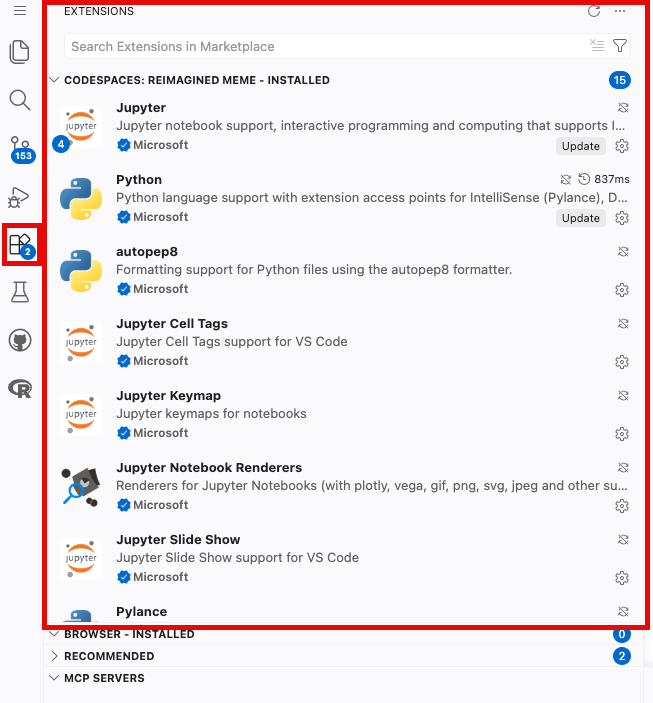
\includegraphics[keepaspectratio]{weeks/week03-r-with-ai/../../assets/images/week3/r1.png}}

\section{Set the AI Model to ``0x''}\label{set-the-ai-model-to-0x}

\begin{enumerate}
\def\labelenumi{\arabic{enumi}.}
\tightlist
\item
  Open the Copilot Chat sidebar (Shortcut: \textbf{Ctrl+Alt+I} or
  \textbf{Cmd+Option+I} on Mac).
\item
  Look for the model selector dropdown at the bottom of the chat window.
\item
  \textbf{Crucial Check:} Choose a model with a \textbf{``0x''
  multiplier} (like GPT-4o 0x). If you do not do this, you will quickly
  run out of your free student quota.

  \begin{itemize}
  \tightlist
  \item
    \emph{Troubleshooting:} If the Chat asks you to ``Sign In'' or
    ``Subscribe,'' your Student Pack is not active. Use your
    institutional login at \texttt{copilot.microsoft.com} or
    authenticate via your university email at
    \texttt{https://m365.cloud.microsoft/chat/}.
  \end{itemize}
\end{enumerate}

\section{Interface Review: Where does R actually
live?}\label{interface-review-where-does-r-actually-live}

To learn R, we are going to start in the ``sandbox.'' Here is how your
screen is laid out:

\begin{itemize}
\tightlist
\item
  \textbf{The Console (Bottom):} Your \textbf{Engine Room}. \emph{Start
  here!} This is where you can type R commands directly next to the
  \texttt{\textgreater{}} prompt and press Enter to see immediate
  results. If you make a mistake, it will show up here in red text.
\item
  \textbf{The Environment (Top Right):} Your \textbf{Work Bench}.
  Whenever you save a piece of data (like a patient's age), it will
  appear in a list here so you can verify R actually ``remembers'' it.
\item
  \textbf{The Explorer (Left Sidebar):} Your \textbf{File Cabinet}. This
  is where you find your \texttt{data/} folder containing your CSV
  files.
\item
  \textbf{The Editor (Top Center):} Your \textbf{Laboratory Notebook}.
  Typing in the Console is great for testing, but it forgets everything
  when you close the window. Later in the lesson, we will use the Editor
  to write and save our permanent code.
\end{itemize}

\section{Interface Review: Working with .qmd and .Rmd
files}\label{interface-review-working-with-.qmd-and-.rmd-files}

When you open a \texttt{.qmd} (Quarto) or \texttt{.Rmd} (RMarkdown)
file, you must know where to look. Here is how your coding workflow maps
to your screen:

\begin{itemize}
\tightlist
\item
  \textbf{The Explorer (Left Sidebar):} Your \textbf{File Cabinet}. This
  is where you find your reports and your \texttt{data/} folder. You
  cannot run code here; you only click files to open them.
\item
  \textbf{The Editor (Top Center):} Your \textbf{Laboratory Notebook}.
  This is where you write your text narrative and your R code.

  \begin{itemize}
  \tightlist
  \item
    \emph{Note:} R code must be placed inside grey \textbf{Code Chunks}
    (starting with
    \texttt{\textasciigrave{}\textasciigrave{}\textasciigrave{}\{r\}}
    and ending with
    \texttt{\textasciigrave{}\textasciigrave{}\textasciigrave{}}). To
    run a chunk, click the small green ``Play'' triangle in the top
    right corner of that specific grey box.
  \end{itemize}
\item
  \textbf{The Console (Bottom):} Your \textbf{Engine Room}. When you
  click the green ``Play'' button in the Editor, the code is sent down
  here to be executed. If there is an error, it will show up here in
  red.

  \begin{itemize}
  \tightlist
  \item
    \emph{Pro Tip:} You can type quick math directly into the console
    (like \texttt{100\ /\ 4}), but it will not be saved in your final
    report.
  \end{itemize}
\item
  \textbf{The Environment (Top Right):} Your \textbf{Work Bench}.
  Whenever you load data or save a calculation, it will appear in a list
  here so you can verify R actually ``remembers'' it.
\end{itemize}

\chapter{Packages (The Toolbox)}\label{packages-the-toolbox}

In R, tools come in ``packages.'' Think of \texttt{install.packages} as
buying a physical toolbox, and \texttt{library()} as opening the lid.

\begin{itemize}
\item
  \textbf{To open your tools:} Type this in your code and run it:

\begin{verbatim}
library(tidyverse) 
\end{verbatim}
\end{itemize}

\begin{quote}
\textbf{Note:} You must run \texttt{library(tidyverse)} every single
time you restart your Codespace.
\end{quote}

\chapter{Basics: Boxes \& Toasters}\label{basics-boxes-toasters}

R is a system of storage (Boxes) and transformation (Toasters).

\section{Variables (The Box)}\label{variables-the-box}

Use \texttt{\textless{}-} to save data into a name.

Code snippet

\begin{verbatim}
Save the number 55 into a variable called patient_age patient_age
\end{verbatim}

\section{Functions (The Toaster)}\label{functions-the-toaster-1}

Functions take input, perform an action, and return output. Look at the
snippet below

Code snippet

\begin{verbatim}
calculate_rectangle_area <- function(length, width) {
  area <- length * width
  return(area)
}

# Example usage:
calculate_rectangle_area(10, 5) # Returns 50
\end{verbatim}

\chapter{Control Flow}\label{control-flow}

\section{The Pipe \%\textgreater\% (The Assembly
Line)}\label{the-pipe-the-assembly-line-1}

The symbol \texttt{\%\textgreater{}\%} means \textbf{``and
then\ldots{}''}.

Both of these lines are identical, which would you prefer to read? (Note
\textbar\textgreater{} is another way to write \%\textgreater\%)

\begin{verbatim}
print(round(sqrt(10), 2))

10 |> sqrt() |> round(2) |> print()
\end{verbatim}

For a real world example of how one may use the pipe

\begin{verbatim}
library(dplyr)

mtcars %>%
  filter(wt > 3) %>%          # 1. Filter for cars heavier than 3,000 lbs
  group_by(cyl) %>%           # 2. Group by number of cylinders
  summarize(avg_mpg = mean(mpg)) # 3. Calculate the average MPG
\end{verbatim}

\section{If / Else (The Fork in the
Road)}\label{if-else-the-fork-in-the-road}

An \textbf{if/else} statement lets the computer make a decision.

The program checks a condition:

\begin{itemize}
\item
  If it is \textbf{TRUE}, it runs one block of code.
\item
  If it is \textbf{FALSE}, it runs another.
\end{itemize}

\begin{verbatim}
temperature <- 5
if (temperature > 10) {
  print("You can wear a t-shirt")
} else {
  print("Wear a jacket")
}
\end{verbatim}

\section{What happens}\label{what-happens}

\begin{enumerate}
\def\labelenumi{\arabic{enumi}.}
\item
  The computer checks: \texttt{temperature\ \textgreater{}\ 10}
\item
  \texttt{5\ \textgreater{}\ 10} is \textbf{FALSE}
\item
  So the \textbf{else} part runs.
\item
  Output:
\end{enumerate}

\begin{verbatim}
"Wear a jacket"
\end{verbatim}

Think of it like a \textbf{fork in the road}:

\begin{itemize}
\item
  One path if the condition is true
\item
  Another path if it's false.
\end{itemize}

\section{Loops (The Treadmill)}\label{loops-the-treadmill-1}

A loop repeats code multiple times.

Instead of writing the same instruction again and again, you let the
computer do it.

\section{Example}\label{example}

\begin{verbatim}
for (i in 1:5) {   
    print(i) 
}
\end{verbatim}

\section{What happens}\label{what-happens-1}

The computer runs the code \textbf{5 times}.

Steps:

\begin{enumerate}
\def\labelenumi{\arabic{enumi}.}
\item
  \texttt{i\ =\ 1} → print 1
\item
  \texttt{i\ =\ 2} → print 2
\item
  \texttt{i\ =\ 3} → print 3
\item
  \texttt{i\ =\ 4} → print 4
\item
  \texttt{i\ =\ 5} → print 5
\end{enumerate}

Output:

\begin{verbatim}
1 2 3 4 5
\end{verbatim}

\section{Audit Check (Important)}\label{audit-check-important}

When using loops, ask:

\textbf{1. Does the loop end?}\\
Bad example (infinite loop):

\begin{verbatim}
while (TRUE) {   print("This never stops") }
\end{verbatim}

\textbf{2. Could this be simpler?}

Sometimes R has built-in functions that replace loops.

Instead of:

\begin{verbatim}
total <- 0 for (i in 1:5) {   total <- total + i }
\end{verbatim}

You can write:

\begin{verbatim}
sum(1:5)
\end{verbatim}

This is \textbf{shorter, safer, and faster}.

\chapter{The Loading Dock (Data
Import)}\label{the-loading-dock-data-import}

Don't type file paths from memory; you will likely make a typo.

\begin{enumerate}
\def\labelenumi{\arabic{enumi}.}
\item
  Find a data file in the \textbf{Explorer} (left sidebar).
\item
  \textbf{Right-click} the file → Select \textbf{Copy Relative Path}.

  \pandocbounded{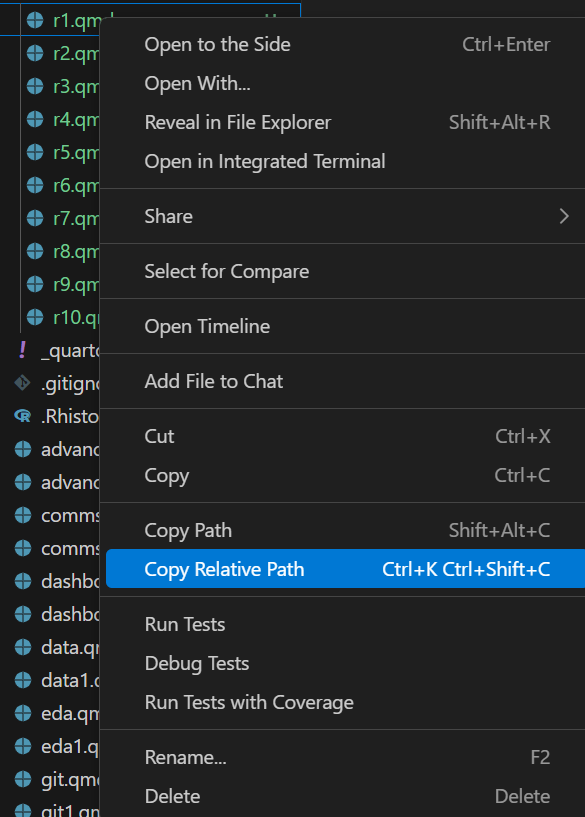
\includegraphics[keepaspectratio]{weeks/week03-r-with-ai/../../assets/images/week3/r5.png}}
\item
  Ask AI: \emph{``Read the CSV at {[}Paste Path Here{]} and save it as
  my\_data.''}
\end{enumerate}

\chapter{The Detective (Debugging)}\label{the-detective-debugging}

AI makes mistakes. When you see \textbf{Red Text} (errors) in the
Console:

\begin{enumerate}
\def\labelenumi{\arabic{enumi}.}
\item
  \textbf{Copy} the Red Text.
\item
  \textbf{Paste} it into Copilot Chat.
\item
  \textbf{Ask:} \emph{``Explain this error and fix the code below:
  {[}Paste Code{]}''}
\end{enumerate}

Try running this line and ask AI why it doesn't work:

\begin{verbatim}
"apple" + 5
\end{verbatim}

\chapter{AI Safety: The Audit
Checklist}\label{ai-safety-the-audit-checklist}

Use this checklist before accepting any AI code:

\begin{itemize}
\item
  \textbf{Spelling:} Are column names spelled exactly as they appear in
  the data?
\item
  \textbf{Case Sensitivity:} Is it \texttt{Age} or \texttt{age}? (R sees
  these as different things).
\item
  \textbf{Missingness:} Did the AI remember \texttt{na.rm\ =\ TRUE} for
  math?
\item
  \textbf{Privacy:} Did the AI try to print the whole dataset
  (potentially exposing patient IDs)?
\end{itemize}

\chapter{The Paper Trail (Comments)}\label{the-paper-trail-comments}

\textbf{The Rule:} Every time you use AI to write code, write a
\texttt{\#} comment in plain English above it explaining what you told
the AI to do.

Code snippet

\begin{verbatim}
# I asked AI to filter for patients with BMI over 30 and count them # [AI CODE BELOW]
\end{verbatim}

Below is an example of non readable code

\begin{verbatim}
# What is x? What is 1.05? Why are we subsetting?
f <- function(x, y) {
z <- x[x$a > y, ]
r <- sum(z$b) * 1.05
return(r)
}

res <- f(df, 100)
\end{verbatim}

And here is an example of readable code

\begin{verbatim}
library(dplyr)

# Calculate the total revenue for high-value orders including a 5% tax
calculate_total_revenue <- function(order_data, minimum_price_threshold) {
  
  sales_tax_rate <- 1.05
  
  total_revenue <- order_data |>
    filter(price > minimum_price_threshold) |>
    summarize(total = sum(price)) |>
    pull(total)
  
  return(total_revenue * sales_tax_rate)
}

# Usage:
final_report_value <- calculate_total_revenue(current_orders, minimum_price_threshold = 100)
\end{verbatim}

Just by reading through each line a reader should understand what is
going on. One does not need to comment every single line, but rather
comment whenever something complex is happening on the code line below
it. And as always source work which is not yours.

\chapter{Assignment: The ``Mad Libs''
Report}\label{assignment-the-mad-libs-report}

\begin{enumerate}
\def\labelenumi{\arabic{enumi}.}
\item
  Open \texttt{week3\_assignment.qmd}.
\item
  Use Copilot to import the Week 1 dataset.
\item
  Use the \textbf{Pipe} to filter and summarize one variable.
\item
  \textbf{Audit:} Add a \texttt{\#} comment explaining your prompt.
\item
  \textbf{Render} the file to HTML.
\item
  \textbf{Commit and Push} to GitHub.
\end{enumerate}

\chapter{Final Summary Checklist}\label{final-summary-checklist}

\begin{itemize}
\item[$\square$]
  Extensions are active (Copilot + R).
\item[$\square$]
  Using \textbf{0x model} in Chat.
\item[$\square$]
  Loaded \texttt{library(tidyverse)}.
\item[$\square$]
  Data imported via \textbf{Relative Path}.
\item[$\square$]
  All code chunks have an \textbf{Audit Comment} (\texttt{\#}).
\item[$\square$]
  Handled \textbf{NA} values correctly.
\item[$\square$]
  Document \textbf{Rendered} and \textbf{Pushed}.
\end{itemize}

\part{Week 4: Git \& Collaboration}

\chapter*{Git \& Collaboration}\label{git-collaboration}
\addcontentsline{toc}{chapter}{Git \& Collaboration}

\markboth{Git \& Collaboration}{Git \& Collaboration}

\section*{Overview}\label{overview-3}
\addcontentsline{toc}{section}{Overview}

\markright{Overview}

\textbf{Summary:} You already know how to save files and make a basic
commit in your Codespace. Now, learn to use Git as a \emph{time machine}
and \emph{collaboration engine} for your analysis---tracking every
change, safely undoing mistakes, working with teammates through branches
and Pull Requests, and keeping a professional audit trail of your
research workflow.

\textbf{Learning Objectives:}

\begin{itemize}
\tightlist
\item
  Distinguish between saving a file and taking a version-control
  ``snapshot'' (commit).
\item
  Read code differences (diffs) to see exactly what changed.
\item
  Use the Codespaces Source Control UI to revert to a previous working
  version.
\item
  Create and switch branches to isolate experimental work.
\item
  Open a Pull Request on GitHub and understand its role in peer review.
\item
  Configure \texttt{.gitignore} and use relative paths for repo hygiene.
\item
  Use AI to translate diffs into clear, professional audit logs.
\item
  Set up a group repository and agree on collaboration norms for the
  term project.
\end{itemize}

\begin{center}\rule{0.5\linewidth}{0.5pt}\end{center}

\section*{\texorpdfstring{\texttt{git1.qmd} Concepts: The ``Save Game''
of Reproducible
Science}{git1.qmd Concepts: The ``Save Game'' of Reproducible Science}}\label{git1.qmd-concepts-the-save-game-of-reproducible-science}
\addcontentsline{toc}{section}{\texttt{git1.qmd} Concepts: The ``Save
Game'' of Reproducible Science}

\markright{\texttt{git1.qmd} Concepts: The ``Save Game'' of Reproducible
Science}

\subsection*{Why Git Matters in Health
Research}\label{why-git-matters-in-health-research}
\addcontentsline{toc}{subsection}{Why Git Matters in Health Research}

\begin{itemize}
\tightlist
\item
  \textbf{The audit trail:} Why \texttt{analysis\_final\_v3.qmd} is
  unsafe in health research; Git gives you a permanent, searchable
  history.
\item
  \textbf{The timeline:} Your repository is a sequence of safe
  checkpoints (commits). Each commit records \emph{who} changed
  \emph{what} and \emph{why}.
\item
  \textbf{Reading the diff:} Red = removed. Green = added. This is the
  visual language of reproducibility.
\end{itemize}

\subsection*{Quick Recap (from Week 2)}\label{quick-recap-from-week-2}
\addcontentsline{toc}{subsection}{Quick Recap (from Week 2)}

You already know how to stage, commit, and sync in your Codespace. This
week, we go deeper: branching, collaboration, and building habits that
will carry through your term project.

\begin{center}\rule{0.5\linewidth}{0.5pt}\end{center}

\section*{\texorpdfstring{\texttt{git2.qmd} Tutorial: Time Travel in
Codespaces}{git2.qmd Tutorial: Time Travel in Codespaces}}\label{git2.qmd-tutorial-time-travel-in-codespaces}
\addcontentsline{toc}{section}{\texttt{git2.qmd} Tutorial: Time Travel
in Codespaces}

\markright{\texttt{git2.qmd} Tutorial: Time Travel in Codespaces}

\emph{Scenario:} We will intentionally break last week's R script and
use Git to rescue it.

\subsection*{Step 1: Confirm Your
Baseline}\label{step-1-confirm-your-baseline}
\addcontentsline{toc}{subsection}{Step 1: Confirm Your Baseline}

Open your \texttt{.qmd} from last week. Make a small, meaningful edit
(e.g., improve a comment). Stage (\textbf{+}), write a descriptive
commit message, and commit (\textbf{✔}). This is your safety net.

\subsection*{Step 2: The Disaster}\label{step-2-the-disaster}
\addcontentsline{toc}{subsection}{Step 2: The Disaster}

Delete a crucial line of R code in a chunk (e.g., the line that loads
the data). \textbf{Save} the file (Ctrl/Cmd + S).

\subsection*{Step 3: Assess the Damage}\label{step-3-assess-the-damage}
\addcontentsline{toc}{subsection}{Step 3: Assess the Damage}

Open \textbf{Source Control} → click the modified file → view the
side-by-side \textbf{diff} to see exactly what changed. Practice reading
the red (removed) and green (added) lines.

\subsection*{Step 4: The Undo Button}\label{step-4-the-undo-button}
\addcontentsline{toc}{subsection}{Step 4: The Undo Button}

Hover over the file name in the Source Control panel and click
\textbf{Discard Changes} (the curved arrow) to restore the file to the
\textbf{last committed} version.

\begin{tcolorbox}[enhanced jigsaw, colframe=quarto-callout-tip-color-frame, toptitle=1mm, colback=white, leftrule=.75mm, toprule=.15mm, colbacktitle=quarto-callout-tip-color!10!white, breakable, bottomrule=.15mm, opacityback=0, title=\textcolor{quarto-callout-tip-color}{\faLightbulb}\hspace{0.5em}{Tip}, rightrule=.15mm, bottomtitle=1mm, opacitybacktitle=0.6, titlerule=0mm, arc=.35mm, left=2mm, coltitle=black]

\textbf{Key takeaway:} Saving writes to disk. Committing writes to
\emph{history}. Only committed work can be recovered by Git.

\end{tcolorbox}

\begin{center}\rule{0.5\linewidth}{0.5pt}\end{center}

\section*{\texorpdfstring{\texttt{git3.qmd} Repo Hygiene:
\texttt{.gitignore} and Relative
Paths}{git3.qmd Repo Hygiene: .gitignore and Relative Paths}}\label{git3.qmd-repo-hygiene-.gitignore-and-relative-paths}
\addcontentsline{toc}{section}{\texttt{git3.qmd} Repo Hygiene:
\texttt{.gitignore} and Relative Paths}

\markright{\texttt{git3.qmd} Repo Hygiene: \texttt{.gitignore} and
Relative Paths}

\subsection*{Why This Matters}\label{why-this-matters}
\addcontentsline{toc}{subsection}{Why This Matters}

As your projects grow, you will generate files that should \emph{not} be
tracked: rendered HTML, temporary data caches, \texttt{.DS\_Store}, API
keys. Tracking these clutters your history and can leak sensitive
information.

\subsection*{\texorpdfstring{\texttt{.gitignore}
Walkthrough}{.gitignore Walkthrough}}\label{gitignore-walkthrough}
\addcontentsline{toc}{subsection}{\texttt{.gitignore} Walkthrough}

\begin{enumerate}
\def\labelenumi{\arabic{enumi}.}
\tightlist
\item
  Open (or create) the \texttt{.gitignore} file in the root of your
  repository.
\item
  Add common patterns:
\end{enumerate}

\begin{verbatim}
# Rendered outputs
*.html
*_files/

# OS junk
.DS_Store
Thumbs.db

# Sensitive
.env
\end{verbatim}

\begin{enumerate}
\def\labelenumi{\arabic{enumi}.}
\setcounter{enumi}{2}
\tightlist
\item
  Stage, commit with a message like
  \texttt{"Add\ .gitignore\ to\ exclude\ rendered\ files"}.
\end{enumerate}

\subsection*{Relative Paths}\label{relative-paths}
\addcontentsline{toc}{subsection}{Relative Paths}

Always use \textbf{relative paths} in your code (e.g.,
\texttt{read.csv("data/nhanes.csv")}), never absolute paths (e.g.,
\texttt{read.csv("/home/user/Documents/nhanes.csv")}). This ensures your
analysis runs on \emph{any} machine---including your grader's Codespace.

\begin{tcolorbox}[enhanced jigsaw, colframe=quarto-callout-warning-color-frame, toptitle=1mm, colback=white, leftrule=.75mm, toprule=.15mm, colbacktitle=quarto-callout-warning-color!10!white, breakable, bottomrule=.15mm, opacityback=0, title=\textcolor{quarto-callout-warning-color}{\faExclamationTriangle}\hspace{0.5em}{Warning}, rightrule=.15mm, bottomtitle=1mm, opacitybacktitle=0.6, titlerule=0mm, arc=.35mm, left=2mm, coltitle=black]

\textbf{Reproducibility rule:} Your term project must run from start to
finish in a \emph{fresh} Codespace. Absolute paths guarantee failure.

\end{tcolorbox}

\begin{center}\rule{0.5\linewidth}{0.5pt}\end{center}

\section*{\texorpdfstring{\texttt{git4.qmd} Branching: Safe
Experimentation}{git4.qmd Branching: Safe Experimentation}}\label{git4.qmd-branching-safe-experimentation}
\addcontentsline{toc}{section}{\texttt{git4.qmd} Branching: Safe
Experimentation}

\markright{\texttt{git4.qmd} Branching: Safe Experimentation}

\subsection*{Concept}\label{concept}
\addcontentsline{toc}{subsection}{Concept}

A \textbf{branch} is a parallel copy of your project. You can experiment
freely on a branch without affecting the stable \texttt{main} version.
When your experiment works, you \textbf{merge} it back.

Think of it like a lab notebook: \texttt{main} is your clean, published
record. A branch is your scratch pad.

\subsection*{Tutorial: Create and Merge a Branch in VS
Code}\label{tutorial-create-and-merge-a-branch-in-vs-code}
\addcontentsline{toc}{subsection}{Tutorial: Create and Merge a Branch in
VS Code}

\subsubsection*{Step 1: Create a Branch}\label{step-1-create-a-branch}
\addcontentsline{toc}{subsubsection}{Step 1: Create a Branch}

\begin{itemize}
\tightlist
\item
  Click the branch name in the bottom-left corner of VS Code (it likely
  says \texttt{main}).
\item
  Select \textbf{Create new branch\ldots{}} and name it something
  descriptive: \texttt{add-age-filter}.
\end{itemize}

\subsubsection*{Step 2: Make Changes on the
Branch}\label{step-2-make-changes-on-the-branch}
\addcontentsline{toc}{subsubsection}{Step 2: Make Changes on the Branch}

\begin{itemize}
\tightlist
\item
  Edit your \texttt{.qmd} (e.g., add a line of code that filters data by
  age).
\item
  Stage and commit on this branch.
\end{itemize}

\subsubsection*{\texorpdfstring{Step 3: Switch Back to
\texttt{main}}{Step 3: Switch Back to main}}\label{step-3-switch-back-to-main}
\addcontentsline{toc}{subsubsection}{Step 3: Switch Back to
\texttt{main}}

\begin{itemize}
\tightlist
\item
  Click the branch name again → select \texttt{main}. Notice your recent
  edits \emph{disappear} from the file. They are safely stored on the
  other branch.
\end{itemize}

\begin{center}\rule{0.5\linewidth}{0.5pt}\end{center}

\section*{\texorpdfstring{\texttt{git5.qmd} Pull Requests: The Peer
Review
Gateway}{git5.qmd Pull Requests: The Peer Review Gateway}}\label{git5.qmd-pull-requests-the-peer-review-gateway}
\addcontentsline{toc}{section}{\texttt{git5.qmd} Pull Requests: The Peer
Review Gateway}

\markright{\texttt{git5.qmd} Pull Requests: The Peer Review Gateway}

\subsection*{What Is a Pull Request?}\label{what-is-a-pull-request}
\addcontentsline{toc}{subsection}{What Is a Pull Request?}

A \textbf{Pull Request (PR)} is a GitHub feature that says: \emph{``I
have changes on a branch. Please review them before they go into
\texttt{main}.''} PRs are how professional teams and researchers
collaborate. You will use them for peer review later in this course.

\subsection*{Tutorial: Open Your First
PR}\label{tutorial-open-your-first-pr}
\addcontentsline{toc}{subsection}{Tutorial: Open Your First PR}

\begin{enumerate}
\def\labelenumi{\arabic{enumi}.}
\tightlist
\item
  After committing changes to a branch (see \texttt{git4.qmd}), click
  \textbf{Sync Changes} to push the branch to GitHub.
\item
  Open your repository on \textbf{github.com}. You should see a banner:
  \emph{``add-age-filter had recent pushes.''} Click \textbf{Compare \&
  pull request}.
\item
  Write a title and short description explaining what you changed and
  why.
\item
  Click \textbf{Create pull request}.
\item
  For now, review the diff on GitHub, then click \textbf{Merge pull
  request} → \textbf{Confirm merge}.
\end{enumerate}

\begin{tcolorbox}[enhanced jigsaw, colframe=quarto-callout-tip-color-frame, toptitle=1mm, colback=white, leftrule=.75mm, toprule=.15mm, colbacktitle=quarto-callout-tip-color!10!white, breakable, bottomrule=.15mm, opacityback=0, title=\textcolor{quarto-callout-tip-color}{\faLightbulb}\hspace{0.5em}{Tip}, rightrule=.15mm, bottomtitle=1mm, opacitybacktitle=0.6, titlerule=0mm, arc=.35mm, left=2mm, coltitle=black]

\textbf{Collaboration norm:} In your term project, agree with your group
that changes go through PRs rather than directly to \texttt{main}. This
creates a built-in review step.

\end{tcolorbox}

\begin{center}\rule{0.5\linewidth}{0.5pt}\end{center}

\section*{\texorpdfstring{\texttt{git6.qmd} AI Auditing for Version
Control}{git6.qmd AI Auditing for Version Control}}\label{git6.qmd-ai-auditing-for-version-control}
\addcontentsline{toc}{section}{\texttt{git6.qmd} AI Auditing for Version
Control}

\markright{\texttt{git6.qmd} AI Auditing for Version Control}

Treat the LLM as a \textbf{Git Translator} that explains diffs and
drafts audit-quality messages.

\subsection*{\texorpdfstring{\texttt{git6a.qmd} Scenario A: Diff
Translation (Pre-Commit
Audit)}{git6a.qmd Scenario A: Diff Translation (Pre-Commit Audit)}}\label{git6a.qmd-scenario-a-diff-translation-pre-commit-audit}
\addcontentsline{toc}{subsection}{\texttt{git6a.qmd} Scenario A: Diff
Translation (Pre-Commit Audit)}

\textbf{Prompt:}

\begin{quote}
``I am about to commit these changes. Explain what I changed in plain
English. Did I delete anything important?''
\end{quote}

Use this to spot accidental deletions or unintended edits before you
commit.

\subsection*{\texorpdfstring{\texttt{git6b.qmd} Scenario B: Auto-Scribe
Commit
Messages}{git6b.qmd Scenario B: Auto-Scribe Commit Messages}}\label{git6b.qmd-scenario-b-auto-scribe-commit-messages}
\addcontentsline{toc}{subsection}{\texttt{git6b.qmd} Scenario B:
Auto-Scribe Commit Messages}

\textbf{Prompt:}

\begin{quote}
``Based on this diff, write a one-sentence, professional commit message
for my Quarto document.''
\end{quote}

Check that the message captures the \textbf{intent} (e.g.,
\texttt{"Filter\ patient\ cohort\ to\ age\ ≥\ 65\ per\ protocol"}), not
just the action (\texttt{"changed\ line\ 42"}).

\subsection*{\texorpdfstring{\texttt{git6c.qmd} Scenario C: Panic
Translator (Error
Handling)}{git6c.qmd Scenario C: Panic Translator (Error Handling)}}\label{git6c.qmd-scenario-c-panic-translator-error-handling}
\addcontentsline{toc}{subsection}{\texttt{git6c.qmd} Scenario C: Panic
Translator (Error Handling)}

\textbf{Prompt:}

\begin{quote}
``VS Code in my GitHub Codespace showed this Git error: {[}paste{]}.
What does it mean in simple terms, and which \textbf{buttons in the VS
Code UI} should I click to fix it?''
\end{quote}

\begin{tcolorbox}[enhanced jigsaw, colframe=quarto-callout-warning-color-frame, toptitle=1mm, colback=white, leftrule=.75mm, toprule=.15mm, colbacktitle=quarto-callout-warning-color!10!white, breakable, bottomrule=.15mm, opacityback=0, title=\textcolor{quarto-callout-warning-color}{\faExclamationTriangle}\hspace{0.5em}{Warning}, rightrule=.15mm, bottomtitle=1mm, opacitybacktitle=0.6, titlerule=0mm, arc=.35mm, left=2mm, coltitle=black]

\textbf{Strict Guardrail:} Never run random terminal commands suggested
by an AI (especially \texttt{-\/-force} or \texttt{reset\ -\/-hard}).
Prefer the VS Code visual interface, which is safer. If the AI suggests
a terminal command, ask it for the GUI equivalent first.

\end{tcolorbox}

\begin{center}\rule{0.5\linewidth}{0.5pt}\end{center}

\section*{\texorpdfstring{\texttt{git7.qmd} Setting Up Your Group
Repository}{git7.qmd Setting Up Your Group Repository}}\label{git7.qmd-setting-up-your-group-repository}
\addcontentsline{toc}{section}{\texttt{git7.qmd} Setting Up Your Group
Repository}

\markright{\texttt{git7.qmd} Setting Up Your Group Repository}

This week you form your term project groups (\textbf{Milestone 0}). Use
this session to establish your collaboration workflow.

\subsection*{Steps}\label{steps-4}
\addcontentsline{toc}{subsection}{Steps}

\begin{enumerate}
\def\labelenumi{\arabic{enumi}.}
\tightlist
\item
  \textbf{One member} creates the group repository from the GitHub
  Classroom link (provided on Canvas).
\item
  All other members accept the invitation and clone the repo by
  launching a Codespace from it.
\item
  As a group, agree on norms:

  \begin{itemize}
  \tightlist
  \item
    All changes go through \textbf{branches → PRs} (no direct pushes to
    \texttt{main}).
  \item
    Commit messages should be descriptive (use the AI auto-scribe
    technique).
  \item
    Keep the repo clean: use \texttt{.gitignore}, relative paths, and a
    clear folder structure.
  \end{itemize}
\item
  Each member makes a small ``hello'' commit (e.g., add your name to the
  \texttt{README.md}) and pushes it to confirm access.
\end{enumerate}

\begin{tcolorbox}[enhanced jigsaw, colframe=quarto-callout-note-color-frame, toptitle=1mm, colback=white, leftrule=.75mm, toprule=.15mm, colbacktitle=quarto-callout-note-color!10!white, breakable, bottomrule=.15mm, opacityback=0, title=\textcolor{quarto-callout-note-color}{\faInfo}\hspace{0.5em}{Note}, rightrule=.15mm, bottomtitle=1mm, opacitybacktitle=0.6, titlerule=0mm, arc=.35mm, left=2mm, coltitle=black]

\textbf{Milestone 0 due Friday:} Confirm your group formation on Canvas
and ensure everyone can commit to the shared repository.

\end{tcolorbox}

\begin{center}\rule{0.5\linewidth}{0.5pt}\end{center}

\section*{\texorpdfstring{\texttt{git8.qmd} Knowledge
Check}{git8.qmd Knowledge Check}}\label{git8.qmd-knowledge-check}
\addcontentsline{toc}{section}{\texttt{git8.qmd} Knowledge Check}

\markright{\texttt{git8.qmd} Knowledge Check}

\begin{enumerate}
\def\labelenumi{\arabic{enumi}.}
\tightlist
\item
  What is the difference between \textbf{saving} a file and
  \textbf{committing} it?
\item
  What does a red line indicate in a diff?
\item
  Which button restores the last \textbf{committed} version of a file?
\item
  Why should you use a \texttt{.gitignore} file?
\item
  What is the purpose of a \textbf{branch}?
\item
  How does a \textbf{Pull Request} support peer review?
\item
  Why are relative paths essential for reproducibility?
\end{enumerate}

\begin{center}\rule{0.5\linewidth}{0.5pt}\end{center}

\section*{\texorpdfstring{\texttt{git9.qmd} Practice Exercise: The Full
Workflow
Drill}{git9.qmd Practice Exercise: The Full Workflow Drill}}\label{git9.qmd-practice-exercise-the-full-workflow-drill}
\addcontentsline{toc}{section}{\texttt{git9.qmd} Practice Exercise: The
Full Workflow Drill}

\markright{\texttt{git9.qmd} Practice Exercise: The Full Workflow Drill}

\begin{enumerate}
\def\labelenumi{\arabic{enumi}.}
\tightlist
\item
  Open your Codespace from last week.
\item
  Create a \texttt{.gitignore} file with sensible defaults for your
  project. \textbf{Commit.}
\item
  Create a new branch called \texttt{practice-edit}.
\item
  On the branch, make a small improvement to your R script (e.g., add a
  clarifying comment or improve a variable name).
\item
  Use an AI model to draft a clear commit message from your diff.
  \textbf{Commit} on the branch.
\item
  Push the branch and open a \textbf{Pull Request} on GitHub.
\item
  Review the PR diff on GitHub, then merge it.
\item
  Back on \texttt{main}, intentionally introduce a breaking typo and
  \textbf{Save}.
\item
  Use \textbf{Discard Changes} to recover the last working version.
\end{enumerate}

\begin{center}\rule{0.5\linewidth}{0.5pt}\end{center}

\section*{\texorpdfstring{\texttt{git10.qmd} Quick Reference: Common Git
Actions in VS
Code}{git10.qmd Quick Reference: Common Git Actions in VS Code}}\label{git10.qmd-quick-reference-common-git-actions-in-vs-code}
\addcontentsline{toc}{section}{\texttt{git10.qmd} Quick Reference:
Common Git Actions in VS Code}

\markright{\texttt{git10.qmd} Quick Reference: Common Git Actions in VS
Code}

\begin{longtable}[]{@{}
  >{\raggedright\arraybackslash}p{(\linewidth - 2\tabcolsep) * \real{0.5000}}
  >{\raggedright\arraybackslash}p{(\linewidth - 2\tabcolsep) * \real{0.5000}}@{}}
\toprule\noalign{}
\begin{minipage}[b]{\linewidth}\raggedright
Action
\end{minipage} & \begin{minipage}[b]{\linewidth}\raggedright
How
\end{minipage} \\
\midrule\noalign{}
\endhead
\bottomrule\noalign{}
\endlastfoot
\textbf{Stage changes} & Source Control → hover file → click
\textbf{+} \\
\textbf{Commit} & Type message → click \textbf{✔} \\
\textbf{View diff} & Click file name in Source Control \\
\textbf{Discard uncommitted edits} & Hover file → click \textbf{curved
arrow} (Discard Changes) \\
\textbf{Create a branch} & Click branch name (bottom-left) →
\textbf{Create new branch\ldots{}} \\
\textbf{Switch branches} & Click branch name → select target branch \\
\textbf{Merge a branch} & Command Palette →
\texttt{Git:\ Merge\ Branch...} \\
\textbf{Push / Sync} & Click \textbf{Sync Changes} in status bar \\
\textbf{Open a Pull Request} & Push branch → go to github.com →
\textbf{Compare \& pull request} \\
\textbf{Add to \texttt{.gitignore}} & Edit \texttt{.gitignore} in repo
root → stage + commit \\
\end{longtable}

\chapter*{Concepts}\label{concepts}
\addcontentsline{toc}{chapter}{Concepts}

\markboth{Concepts}{Concepts}

\begin{itemize}
\item
  \textbf{The Audit Trail:} Git records \emph{who} changed \emph{what}.

  \pandocbounded{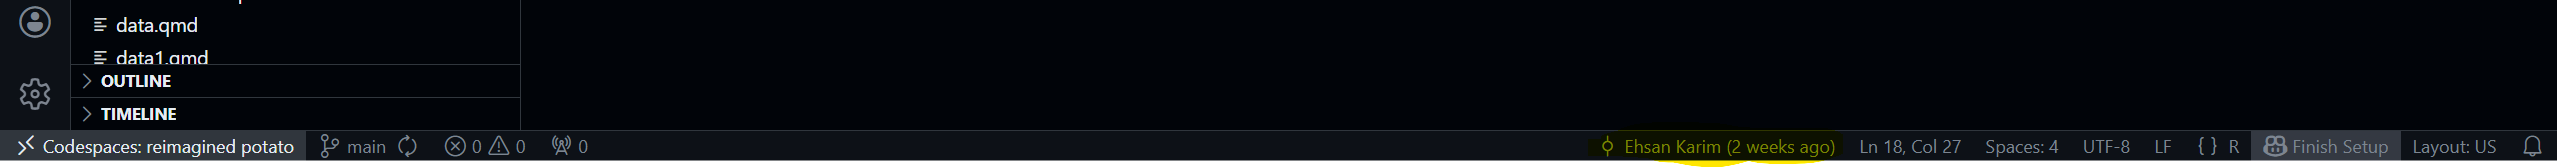
\includegraphics[keepaspectratio]{weeks/week04-git-collaboration/../../assets/images/git1/git1_1.png}}

  Selecting any line will show who changed that line and when they did
  so.
\item
  \textbf{The Timeline:} A sequence of safe checkpoints (commits). This
  shows the reason behind each change and what was change. These
  checkpoints can always be reverted back to if the need be.

  \begin{figure}[H]

  {\centering \pandocbounded{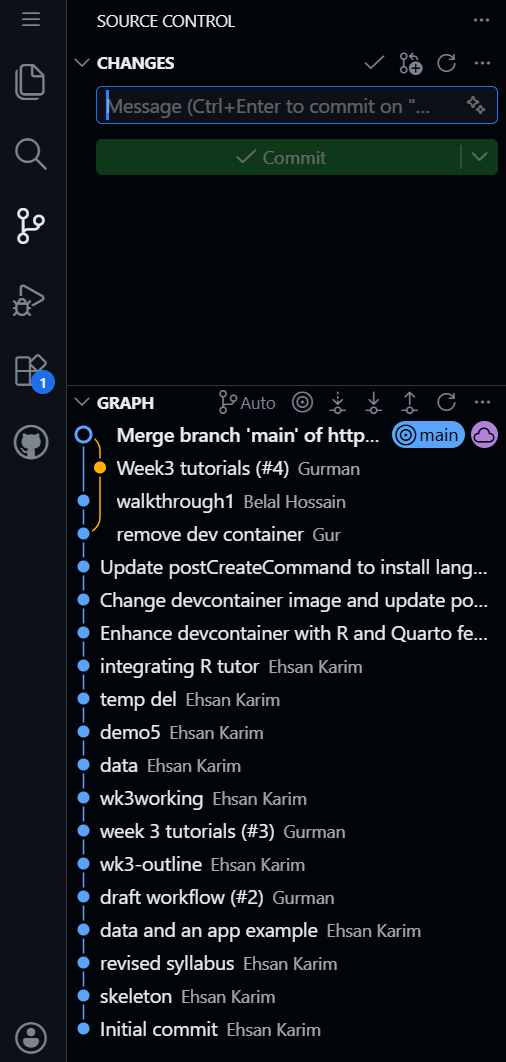
\includegraphics[keepaspectratio]{weeks/week04-git-collaboration/../../assets/images/git1/git1_2.png}}

  }

  \caption{This tree shows every commit (checkpoints)}

  \end{figure}%
\item
  \textbf{The Language of Diffs:}

  \begin{itemize}
  \item
    \texttt{Red\ (-)}: Removed lines.
  \item
    \texttt{Green\ (+)}: Added lines.

    \pandocbounded{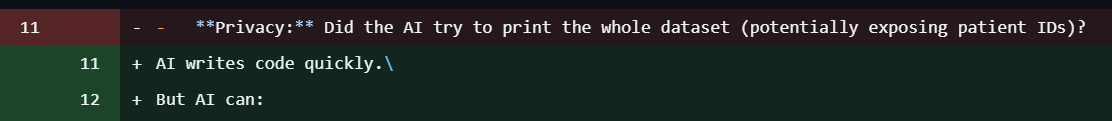
\includegraphics[keepaspectratio]{weeks/week04-git-collaboration/../../assets/images/git1/git1_3.png}}

    Observbing this image, we see that line 11 was replaced, the old
    data on line 11 is colored red, while the new changes are shown in
    green.
  \end{itemize}
\end{itemize}

\begin{quote}
\textbf{Key Rule:} Saving writes to disk on your commuter. Committing
and pushing to the repo writes to history.
\end{quote}

\chapter*{Tutorial}\label{tutorial}
\addcontentsline{toc}{chapter}{Tutorial}

\markboth{Tutorial}{Tutorial}

Follow these steps

\begin{enumerate}
\def\labelenumi{\arabic{enumi}.}
\item
  \textbf{Edit:} Make a change to your code, any file in the repo will
  do, and save the file.

  \pandocbounded{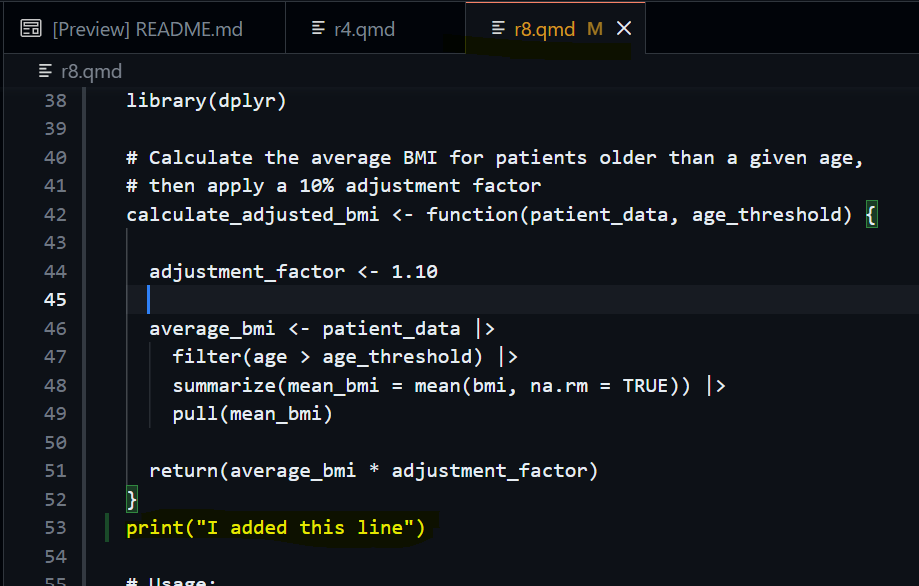
\includegraphics[keepaspectratio]{weeks/week04-git-collaboration/../../assets/images/git2/git2_1.png}}

  Key things to note are that the open file tab has changed colors, this
  shows that github has acknowledged that the file has been changed.
\item
  \textbf{Commit:} Stage and Commit in the Source Control tab.

  As we have seen from the previous tutorial, open up the git tab as
  indicated by the orange-peach highlight. When a file is changed you
  will be presented with the screen below.

  \textbf{To stage a change, press the + icon.}

  \pandocbounded{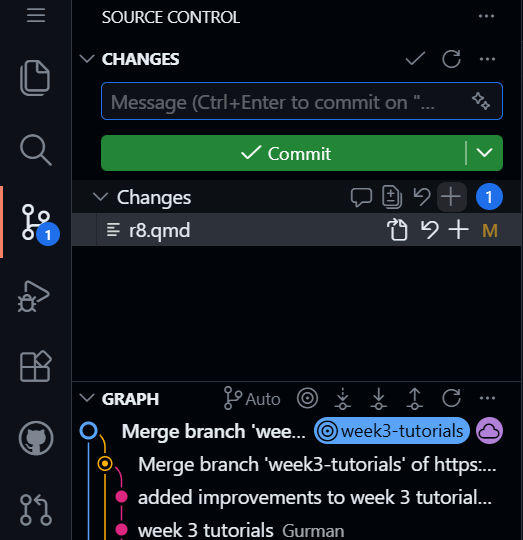
\includegraphics[keepaspectratio]{weeks/week04-git-collaboration/../../assets/images/git2/git2_2.png}}

  Your menu should look like this now;

  \pandocbounded{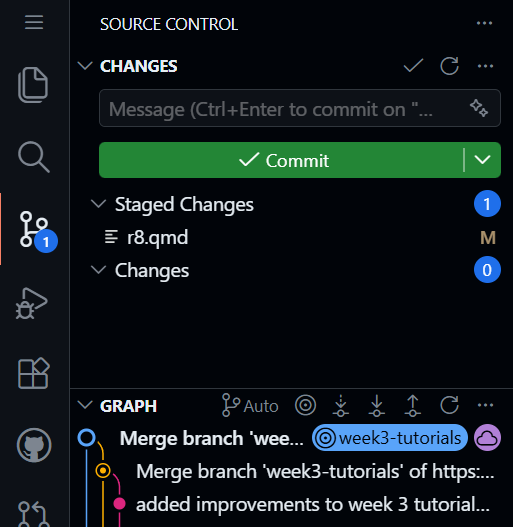
\includegraphics[keepaspectratio]{weeks/week04-git-collaboration/../../assets/images/git2/git2_3.png}}

  Then when you are ready to commit, you can click the big green button!
  You can also click the down arrow on the big green button to see more
  options, as well as the commit option. We will discuss those other
  options later.

  \pandocbounded{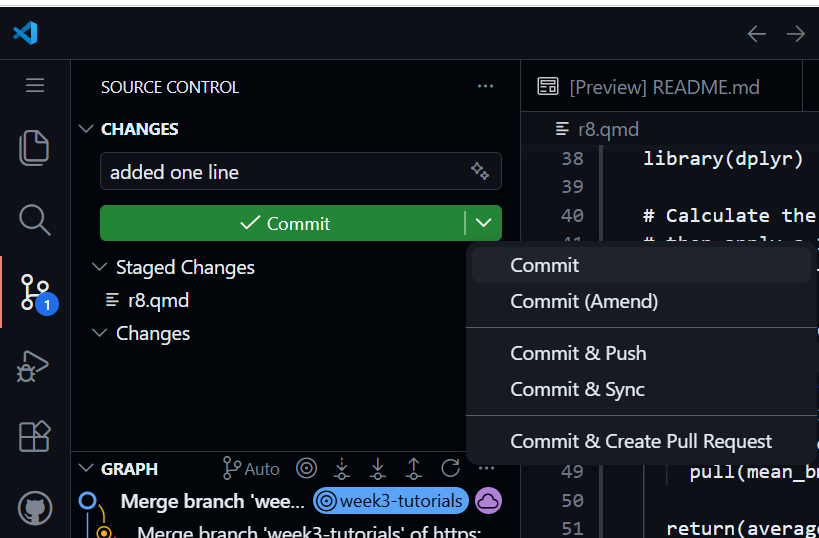
\includegraphics[keepaspectratio]{weeks/week04-git-collaboration/../../assets/images/git2/git2_4.png}}
\item
  \textbf{Break:} Delete the code you just added and save.

  \pandocbounded{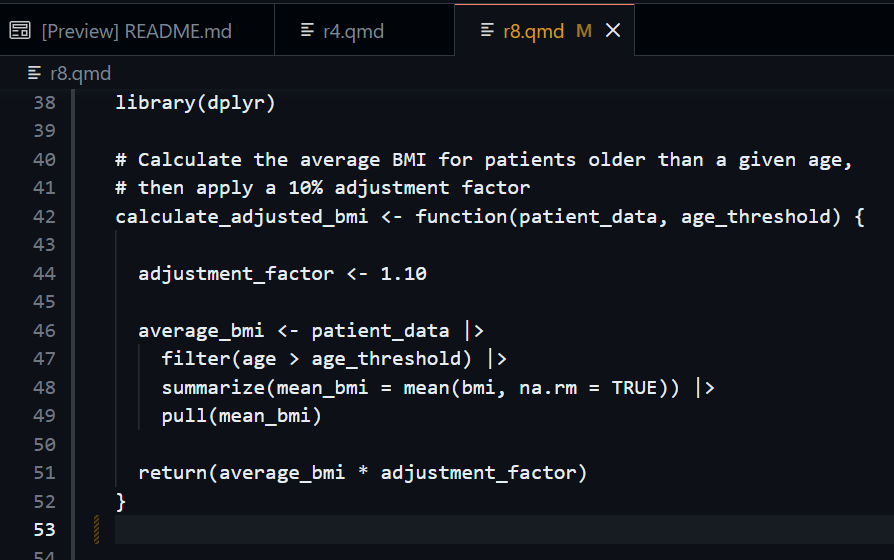
\includegraphics[keepaspectratio]{weeks/week04-git-collaboration/../../assets/images/git2/git2_5.png}}
\item
  \textbf{Rescue:} Hover over the file in Source Control again, click
  the \textbf{Discard Changes} option.

  \pandocbounded{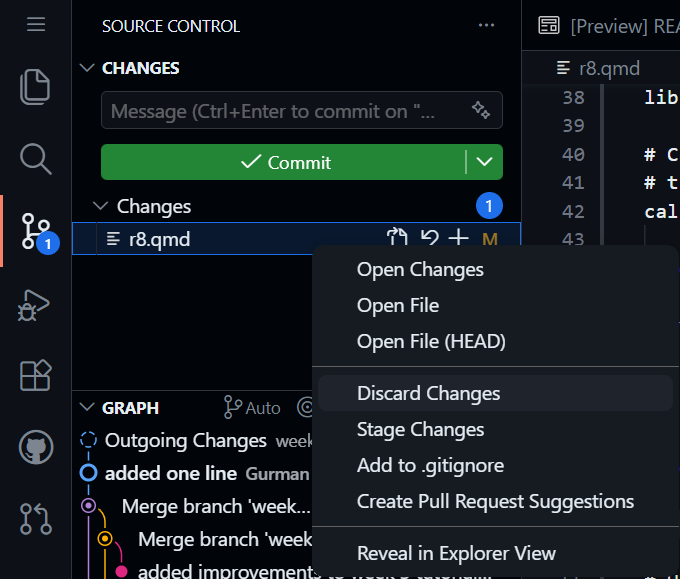
\includegraphics[keepaspectratio]{weeks/week04-git-collaboration/../../assets/images/git2/git2_6.png}}

  This will revert the file back to what it was before. This can recover
  data that your computer potentially cannot, its a very powerful in git
  and showcases one aspect of how git operates. It is a record of all
  your work and saved chunks.
\end{enumerate}

\chapter*{Repo Hygiene}\label{repo-hygiene}
\addcontentsline{toc}{chapter}{Repo Hygiene}

\markboth{Repo Hygiene}{Repo Hygiene}

\subsubsection*{.gitignore}\label{gitignore}
\addcontentsline{toc}{subsubsection}{.gitignore}

Sometimes there are files you do not want to be tracked by github. This
could be anything from files specific to your computer to items like
patient data which should not be stored on the cloud unless allowed so
by policy.

\begin{enumerate}
\def\labelenumi{\arabic{enumi}.}
\item
  Create a file named \texttt{.gitignore} in your root directory: It has
  to be this exact spelling for git to recognize it.

  \pandocbounded{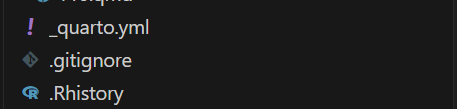
\includegraphics[keepaspectratio]{weeks/week04-git-collaboration/../../assets/images/git3/git3_1.png}}

  You will know its correct when it has its own icon as seen above
\item
  Then create a new file, any type will do but for this lesson I will
  create a text file called dont\_want\_tracked

  \pandocbounded{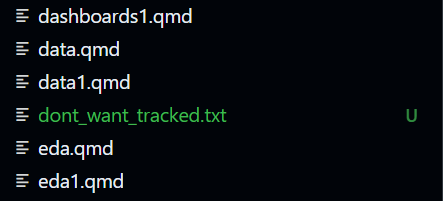
\includegraphics[keepaspectratio]{weeks/week04-git-collaboration/../../assets/images/git3/git3_2.png}}
\item
  Then open the gitignore file and add the name of the file you dont
  want tracked into it.

  \pandocbounded{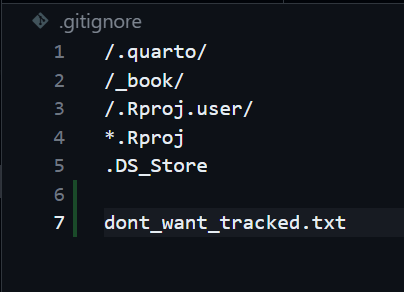
\includegraphics[keepaspectratio]{weeks/week04-git-collaboration/../../assets/images/git3/git3_4.png}}
\item
  Now you will see the new file, which was green is now grayed out. This
  shows that github is no longer tracking it and coloring it green
  (which it does for new files).

  \pandocbounded{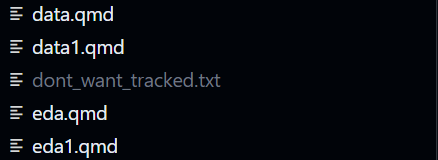
\includegraphics[keepaspectratio]{weeks/week04-git-collaboration/../../assets/images/git3/git3_5.png}}
\end{enumerate}

This is simple enough right? Whenever in doubt, ask AI how to stop a
file from being tracked by git and it will offer some advice. Now stage
and commit this like we have done in the previous tutorial.

\subsubsection*{Realative Paths}\label{realative-paths}
\addcontentsline{toc}{subsubsection}{Realative Paths}

Always use relative paths in your code (e.g.,
read.csv(``data/nhanes.csv'')), never absolute paths (e.g.,
read.csv(``/home/user/Documents/nhanes.csv'')). This ensures your
analysis runs on any machine---including your grader's Codespace.

Reproducibility rule: Your term project must run from start to finish in
a fresh Codespace. Absolute paths guarantee failure.

\chapter*{Branching}\label{branching}
\addcontentsline{toc}{chapter}{Branching}

\markboth{Branching}{Branching}

\begin{enumerate}
\def\labelenumi{\arabic{enumi}.}
\tightlist
\item
  \textbf{Create:}
\end{enumerate}

Click branch name (bottom-left).

\pandocbounded{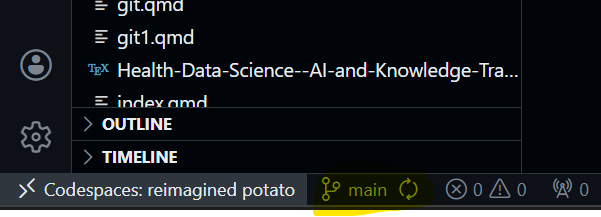
\includegraphics[keepaspectratio]{weeks/week04-git-collaboration/../../assets/images/git4/git4_1.png}}

This will pop up a menu where you have the option to
\texttt{Create\ new\ branch}.

\pandocbounded{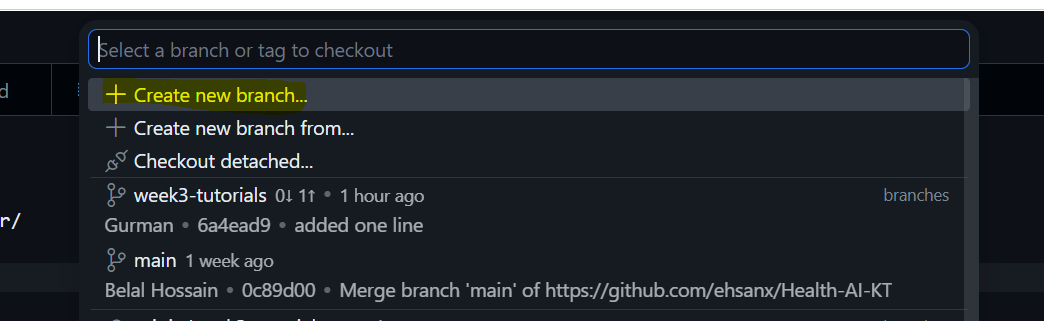
\includegraphics[keepaspectratio]{weeks/week04-git-collaboration/../../assets/images/git4/git4_2.png}}

Select this and call it first-branch. Note branch names may not have any
spaces and limited special characters, the system will let you know if a
name is invalid.

\pandocbounded{
\includegraphics[keepaspectratio]{weeks/week04-git-collaboration/../../assets/images/git4/git4_3.png}}

\begin{enumerate}
\def\labelenumi{\arabic{enumi}.}
\setcounter{enumi}{1}
\item
  \textbf{Work:} Make changes, like those in the previous tutorial and
  commit your changes on your branch.
\item
  \textbf{Switch:} Click the branch button on the bottom left again and
  once this menu pops up, select \texttt{main}. Note that your changes
  vanish (they are safely in the other branch). If you decide to switch
  back to your branch, your changes will reappear. This is amazing for
  multitasking on different features and keeping code clean.

  \pandocbounded{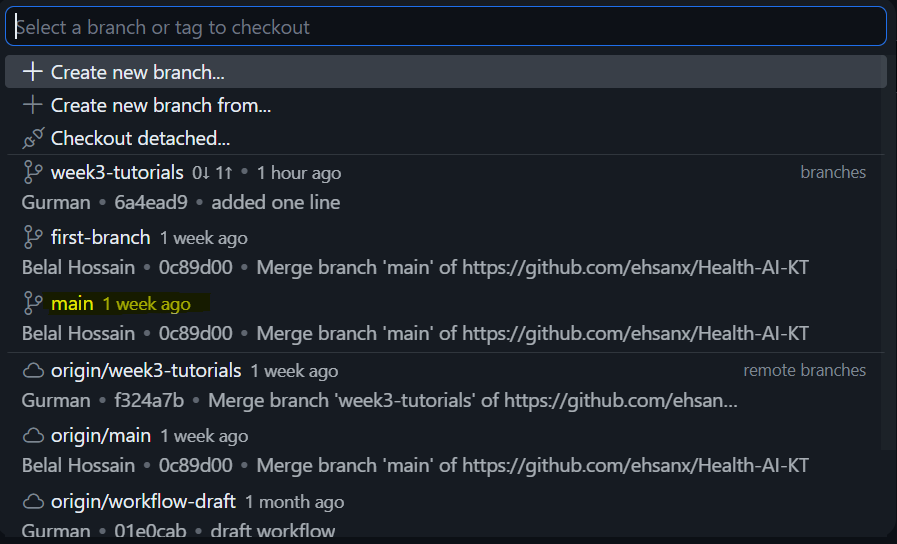
\includegraphics[keepaspectratio]{weeks/week04-git-collaboration/../../assets/images/git4/git4_5.png}}
\end{enumerate}

\chapter*{Pull Requests}\label{pull-requests}
\addcontentsline{toc}{chapter}{Pull Requests}

\markboth{Pull Requests}{Pull Requests}

A \textbf{Pull Request (PR)} is a GitHub feature that says: \emph{``I
have changes on a branch. Please review them before they go into
\texttt{main}.''} PRs are how professional teams and researchers
collaborate. You will use them for peer review later in this course.
This is also the best way to merge your own changes into main, as it
forces you to see what has been change and allows one to check what they
are submitting to the main branch, the backbone or ``trunck'' of the
tree

\begin{enumerate}
\def\labelenumi{\arabic{enumi}.}
\item
  \textbf{Sync:} Click ``Sync Changes'' to push your branch to GitHub.
  This can be blue or green or say publish branch or not. Whichever the
  case, clicking this button will make everything on your computer
  update to the online github repo.

  \pandocbounded{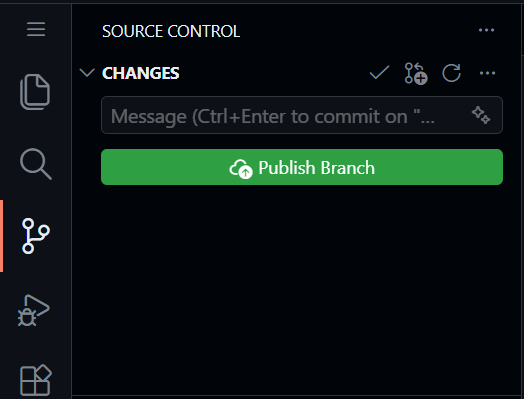
\includegraphics[keepaspectratio]{weeks/week04-git-collaboration/../../assets/images/git5/git5_1.png}}
\item
  \textbf{PR:} Go to your repo on github online and click ``Compare \&
  pull request.''

  \pandocbounded{
\includegraphics[keepaspectratio]{weeks/week04-git-collaboration/../../assets/images/git5/git5_3.png}}

  We are then presented with the screen below. Press the big green
  button ``New Pull Request''

  \pandocbounded{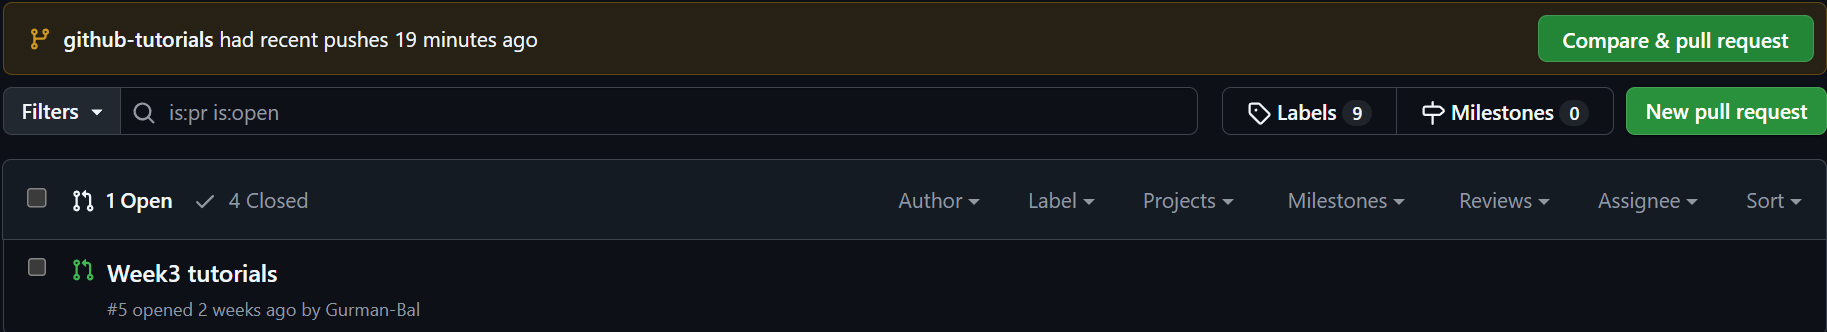
\includegraphics[keepaspectratio]{weeks/week04-git-collaboration/../../assets/images/git5/git5_2.png}}

  Then you are presented this menu. This shows all the different
  branches that can be merged into main. Select on the one you want to
  merge into main.

  \pandocbounded{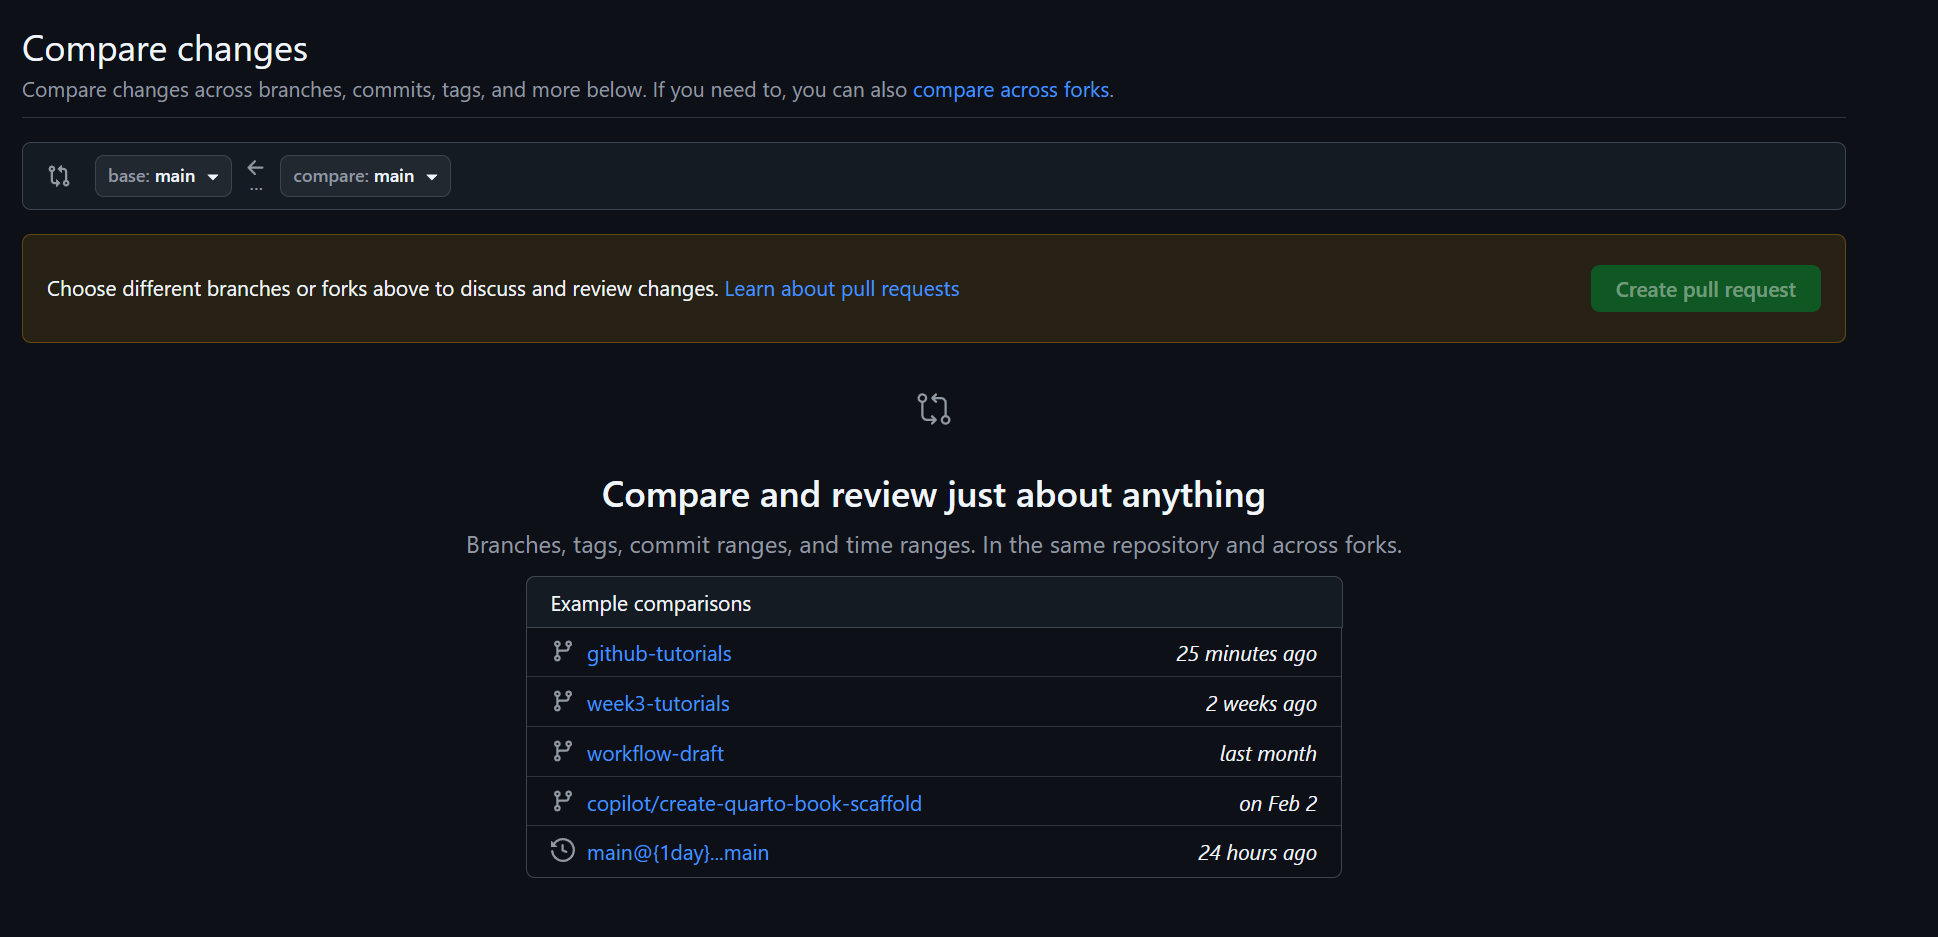
\includegraphics[keepaspectratio]{weeks/week04-git-collaboration/../../assets/images/git5/git5_4.png}}

  Once you select the one, you can make a pull request! Select this.

  \pandocbounded{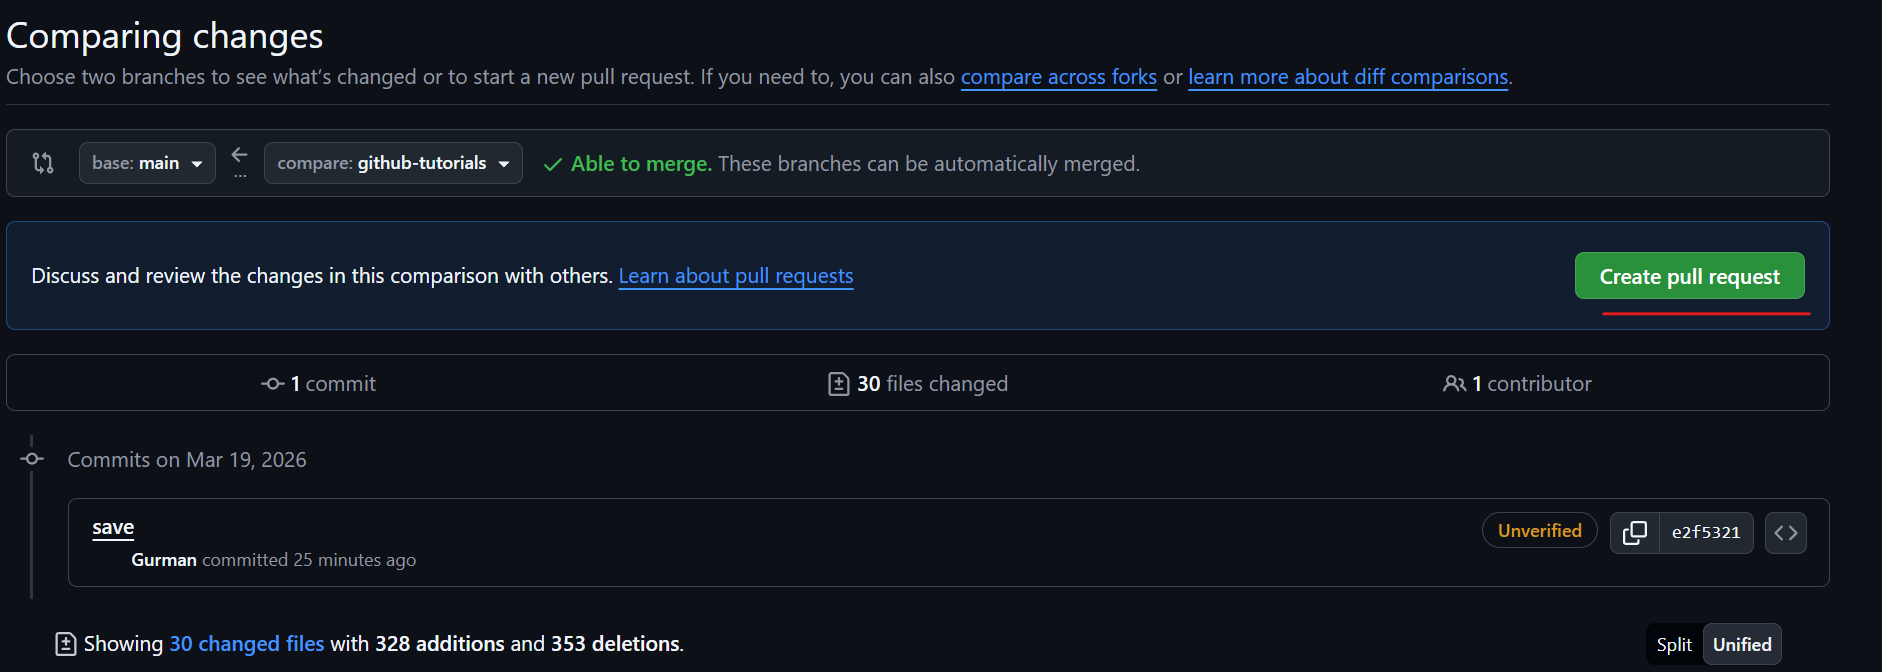
\includegraphics[keepaspectratio]{weeks/week04-git-collaboration/../../assets/images/git5/git5_5.png}}
\item
  \textbf{Merge:} Review the diff, then click ``Merge pull request.'' If
  there are merge conflicts, ask AI the best way to resolve them.

  \pandocbounded{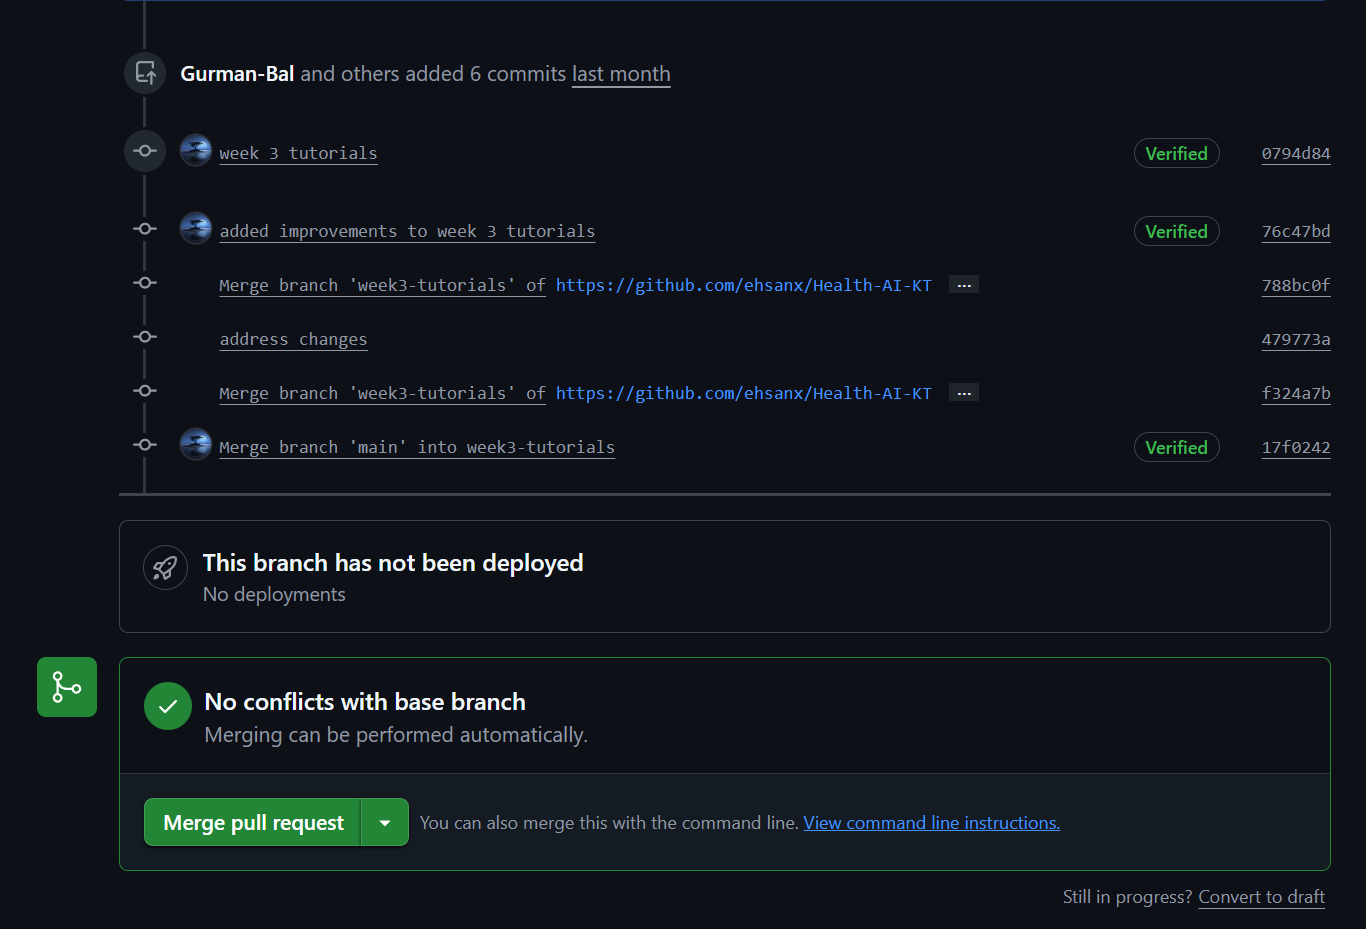
\includegraphics[keepaspectratio]{weeks/week04-git-collaboration/../../assets/images/git5/git6_6.png}}
\end{enumerate}

\chapter*{AI Auditing}\label{ai-auditing}
\addcontentsline{toc}{chapter}{AI Auditing}

\markboth{AI Auditing}{AI Auditing}

Use these prompts with your AI assistant:

\begin{itemize}
\item
  \textbf{Audit:} ``I am about to commit these changes. Explain what I
  changed in plain English. Did I delete anything important?''

  Use this to spot accidental deletions or unintended edits before you
  commit.
\item
  \textbf{Scribe:} ``Based on this diff, write a one-sentence,
  professional commit message for my Quarto document.''

  Check that the message captures the \textbf{intent} (e.g.,
  \texttt{"Filter\ patient\ cohort\ to\ age\ ≥\ 65\ per\ protocol"}),
  not just the action (\texttt{"changed\ line\ 42"}).
\item
  \textbf{Panic:} ``VS Code shows this error: {[}PASTE ERROR{]}. What
  does it mean in simple terms and what buttons should I click?''

  Never run random terminal commands suggested by an AI (especially
  \texttt{-\/-force} or \texttt{reset\ -\/-hard}). Prefer the VS Code
  visual interface, which is safer. If the AI suggests a terminal
  command, ask it for the GUI equivalent first.
\end{itemize}

\chapter*{Setting Up Your Group
Repository}\label{setting-up-your-group-repository}
\addcontentsline{toc}{chapter}{Setting Up Your Group Repository}

\markboth{Setting Up Your Group Repository}{Setting Up Your Group
Repository}

\begin{enumerate}
\def\labelenumi{\arabic{enumi}.}
\tightlist
\item
  \textbf{Invite:} One member creates the repo; others accept the
  invite.
\item
  \textbf{Clone:} Everyone launches their own Codespace.
\item
  \textbf{Norms:} Agree: ``No direct pushes to \texttt{main}.''
\item
  \textbf{Test:} Everyone makes a \texttt{README.md} update to confirm
  access.
\end{enumerate}

\chapter*{Knowledge Check}\label{knowledge-check}
\addcontentsline{toc}{chapter}{Knowledge Check}

\markboth{Knowledge Check}{Knowledge Check}

\begin{enumerate}
\def\labelenumi{\arabic{enumi}.}
\tightlist
\item
  \textbf{Saving vs.~Committing:} Saving = disk; Committing = history.
\item
  \textbf{Red line:} Deletion.
\item
  \textbf{Restore:} Discard Changes button.
\item
  \textbf{.gitignore:} Prevents tracking junk/secrets.
\item
  \textbf{Branch:} Parallel experimental workspace.
\item
  \textbf{PR:} A peer review workflow for merging code.
\item
  \textbf{Relative Paths:} Ensures the project runs on any machine.
\end{enumerate}

\chapter*{Practice Exercise: Full
Workflow}\label{practice-exercise-full-workflow}
\addcontentsline{toc}{chapter}{Practice Exercise: Full Workflow}

\markboth{Practice Exercise: Full Workflow}{Practice Exercise: Full
Workflow}

\begin{longtable}[]{@{}lll@{}}
\toprule\noalign{}
Step & Task & Done \\
\midrule\noalign{}
\endhead
\bottomrule\noalign{}
\endlastfoot
1 & Edit Code & {[} {]} \\
2 & Create Branch & {[} {]} \\
3 & AI Draft Msg & {[} {]} \\
4 & Stage \& Commit & {[} {]} \\
5 & Push \& PR & {[} {]} \\
6 & Merge & {[} {]} \\
\end{longtable}

\chapter*{Quick Reference}\label{quick-reference}
\addcontentsline{toc}{chapter}{Quick Reference}

\markboth{Quick Reference}{Quick Reference}

\begin{longtable}[]{@{}
  >{\raggedright\arraybackslash}p{(\linewidth - 2\tabcolsep) * \real{0.1528}}
  >{\raggedright\arraybackslash}p{(\linewidth - 2\tabcolsep) * \real{0.8472}}@{}}
\toprule\noalign{}
\begin{minipage}[b]{\linewidth}\raggedright
Action
\end{minipage} & \begin{minipage}[b]{\linewidth}\raggedright
How-To
\end{minipage} \\
\midrule\noalign{}
\endhead
\bottomrule\noalign{}
\endlastfoot
Stage & Source Control (+) \\
Commit & Type msg + ✔ \\
View Diff & Click file in Source Control \\
Discard & Left click file in source control and click discard changes \\
Branch & Bottom-left status bar \\
Sync & Sync Changes button \\
\end{longtable}

\part{Week 5: Polyglot Awareness \& R Deepening}

\chapter*{Python with AI}\label{python-with-ai}
\addcontentsline{toc}{chapter}{Python with AI}

\markboth{Python with AI}{Python with AI}

\section*{Overview}\label{overview-4}
\addcontentsline{toc}{section}{Overview}

\markright{Overview}

\textbf{Summary:} You know how to wrangle data in R (Week 3) and track
your history with Git (Week 4). This week, you'll use Large Language
Models to translate your existing R skills into Python---running
everything inside your GitHub Codespace. You don't need to become a
Python expert; you need to be great at \emph{directing the AI} and
\emph{verifying the output}.

\textbf{Learning Objectives:}

\begin{itemize}
\tightlist
\item
  Explain when and why a health data scientist might choose Python over
  R (and vice versa).
\item
  Create and run a Python Jupyter Notebook (\texttt{.ipynb}) and a
  Python script (\texttt{.py}) in your Codespace.
\item
  Use the VS Code \textbf{Variables} pane and Data Viewer to inspect
  Python data.
\item
  Map R mental models to Python equivalents (\texttt{dplyr} →
  \texttt{pandas}, \texttt{ggplot2} →
  \texttt{seaborn}/\texttt{matplotlib}).
\item
  Manage a reproducible Python environment using
  \texttt{requirements.txt}.
\item
  Use \texttt{reticulate} to call R from Python (or vice versa) for a
  simple interoperability demo.
\item
  Avoid ``Frankenstein code'' via the \textbf{One Step, One Cell} AI
  workflow.
\item
  Apply Week 4 Git skills to track Python translations with meaningful
  commits.
\end{itemize}

\begin{center}\rule{0.5\linewidth}{0.5pt}\end{center}

\section*{\texorpdfstring{\texttt{python1.qmd} Concepts: Python vs
R---When and
Why?}{python1.qmd Concepts: Python vs R---When and Why?}}\label{python1.qmd-concepts-python-vs-rwhen-and-why}
\addcontentsline{toc}{section}{\texttt{python1.qmd} Concepts: Python vs
R---When and Why?}

\markright{\texttt{python1.qmd} Concepts: Python vs R---When and Why?}

\subsection*{Two Languages, One
Codespace}\label{two-languages-one-codespace}
\addcontentsline{toc}{subsection}{Two Languages, One Codespace}

Both R and Python are first-class citizens in your GitHub Codespace. You
are not choosing one forever; you are learning when each is the better
tool.

\begin{longtable}[]{@{}
  >{\raggedright\arraybackslash}p{(\linewidth - 4\tabcolsep) * \real{0.3333}}
  >{\raggedright\arraybackslash}p{(\linewidth - 4\tabcolsep) * \real{0.3333}}
  >{\raggedright\arraybackslash}p{(\linewidth - 4\tabcolsep) * \real{0.3333}}@{}}
\toprule\noalign{}
\begin{minipage}[b]{\linewidth}\raggedright
Strength
\end{minipage} & \begin{minipage}[b]{\linewidth}\raggedright
R
\end{minipage} & \begin{minipage}[b]{\linewidth}\raggedright
Python
\end{minipage} \\
\midrule\noalign{}
\endhead
\bottomrule\noalign{}
\endlastfoot
Statistical modeling \& \texttt{tidyverse}-style wrangling & Mature
ecosystem (\texttt{dplyr}, \texttt{ggplot2}, \texttt{lme4}) & Possible,
but more verbose \\
Machine learning \& deep learning & Growing (\texttt{tidymodels},
\texttt{torch}) & Dominant (\texttt{scikit-learn}, \texttt{tensorflow},
\texttt{pytorch}) \\
Dashboards & Shiny (Week 8) & Streamlit, Dash \\
General-purpose scripting \& automation & Less common & Very common \\
\end{longtable}

\textbf{Bottom line for this course:} R remains your primary analysis
language. Python is introduced so you can (a) read and adapt Python code
you encounter in the wild, (b) leverage Python-only libraries when
needed, and (c) demonstrate bilingual fluency in your portfolio.

\subsection*{Notebooks vs Scripts}\label{notebooks-vs-scripts}
\addcontentsline{toc}{subsection}{Notebooks vs Scripts}

\begin{itemize}
\tightlist
\item
  \textbf{Notebook (\texttt{.ipynb}):} Best for exploration, teaching,
  and narrative analysis. Cells run interactively; output appears
  inline.
\item
  \textbf{Script (\texttt{.py}):} Best for reusable utilities,
  automation, and clean code. Runs top-to-bottom.
\end{itemize}

In this week's activities, you will work primarily in a notebook but
also create one short \texttt{.py} script to see the difference.

\begin{center}\rule{0.5\linewidth}{0.5pt}\end{center}

\section*{\texorpdfstring{\texttt{python2.qmd} Setup: Jupyter in
Codespaces}{python2.qmd Setup: Jupyter in Codespaces}}\label{python2.qmd-setup-jupyter-in-codespaces}
\addcontentsline{toc}{section}{\texttt{python2.qmd} Setup: Jupyter in
Codespaces}

\markright{\texttt{python2.qmd} Setup: Jupyter in Codespaces}

\subsection*{Create and Run a Notebook}\label{create-and-run-a-notebook}
\addcontentsline{toc}{subsection}{Create and Run a Notebook}

\begin{enumerate}
\def\labelenumi{\arabic{enumi}.}
\tightlist
\item
  \textbf{New file:} VS Code Explorer → \textbf{New File} → name it
  \texttt{translation.ipynb}.
\item
  \textbf{Select kernel:} Notebook toolbar → \textbf{Select Kernel} →
  choose the recommended Python environment.
\item
  \textbf{First cell:} Type \texttt{print("Hello\ from\ Python")} and
  press \textbf{Shift + Enter}.
\end{enumerate}

\subsection*{The Variables Pane and Data
Viewer}\label{the-variables-pane-and-data-viewer}
\addcontentsline{toc}{subsection}{The Variables Pane and Data Viewer}

After running a cell that creates a variable, open the
\textbf{Variables} pane (notebook toolbar). Double-click any DataFrame
to open an ``Excel-like'' grid view---your best friend for verifying
that data loaded correctly.

\begin{tcolorbox}[enhanced jigsaw, colframe=quarto-callout-tip-color-frame, toptitle=1mm, colback=white, leftrule=.75mm, toprule=.15mm, colbacktitle=quarto-callout-tip-color!10!white, breakable, bottomrule=.15mm, opacityback=0, title=\textcolor{quarto-callout-tip-color}{\faLightbulb}\hspace{0.5em}{Tip}, rightrule=.15mm, bottomtitle=1mm, opacitybacktitle=0.6, titlerule=0mm, arc=.35mm, left=2mm, coltitle=black]

If notebook features (Variables, Data Viewer) are missing, ensure the
\textbf{Jupyter} extension is enabled in your Codespace. Check the
Extensions panel (block icon on the left sidebar).

\end{tcolorbox}

\begin{center}\rule{0.5\linewidth}{0.5pt}\end{center}

\section*{\texorpdfstring{\texttt{python3.qmd} Packages and Environment
Hygiene}{python3.qmd Packages and Environment Hygiene}}\label{python3.qmd-packages-and-environment-hygiene}
\addcontentsline{toc}{section}{\texttt{python3.qmd} Packages and
Environment Hygiene}

\markright{\texttt{python3.qmd} Packages and Environment Hygiene}

\subsection*{\texorpdfstring{R \texttt{library()} → Python
\texttt{import}}{R library() → Python import}}\label{r-library-python-import}
\addcontentsline{toc}{subsection}{R \texttt{library()} → Python
\texttt{import}}

\begin{longtable}[]{@{}
  >{\raggedright\arraybackslash}p{(\linewidth - 2\tabcolsep) * \real{0.5000}}
  >{\raggedright\arraybackslash}p{(\linewidth - 2\tabcolsep) * \real{0.5000}}@{}}
\toprule\noalign{}
\begin{minipage}[b]{\linewidth}\raggedright
R
\end{minipage} & \begin{minipage}[b]{\linewidth}\raggedright
Python equivalent
\end{minipage} \\
\midrule\noalign{}
\endhead
\bottomrule\noalign{}
\endlastfoot
\texttt{library(dplyr)} / tidyverse & \texttt{import\ pandas\ as\ pd} \\
\texttt{library(ggplot2)} & \texttt{import\ seaborn\ as\ sns} or
\texttt{import\ matplotlib.pyplot\ as\ plt} \\
\texttt{library(readr)} & \texttt{pd.read\_csv(...)} (built into
pandas) \\
\end{longtable}

\subsection*{\texorpdfstring{Why \texttt{requirements.txt}
Matters}{Why requirements.txt Matters}}\label{why-requirements.txt-matters}
\addcontentsline{toc}{subsection}{Why \texttt{requirements.txt} Matters}

Your course Codespace comes with core packages pre-installed. But your
\textbf{term project must run in a fresh Codespace}. If you add a
package, you must record it:

\begin{enumerate}
\def\labelenumi{\arabic{enumi}.}
\tightlist
\item
  Open (or create) \texttt{requirements.txt} in your repo root.
\item
  Add the package name and version:
\end{enumerate}

\begin{verbatim}
pandas==2.2.0
seaborn==0.13.2
\end{verbatim}

\begin{enumerate}
\def\labelenumi{\arabic{enumi}.}
\setcounter{enumi}{2}
\tightlist
\item
  To install from this file: the Codespace setup script runs
  \texttt{pip\ install\ -r\ requirements.txt} automatically on launch.
\end{enumerate}

\begin{tcolorbox}[enhanced jigsaw, colframe=quarto-callout-warning-color-frame, toptitle=1mm, colback=white, leftrule=.75mm, toprule=.15mm, colbacktitle=quarto-callout-warning-color!10!white, breakable, bottomrule=.15mm, opacityback=0, title=\textcolor{quarto-callout-warning-color}{\faExclamationTriangle}\hspace{0.5em}{Warning}, rightrule=.15mm, bottomtitle=1mm, opacitybacktitle=0.6, titlerule=0mm, arc=.35mm, left=2mm, coltitle=black]

\textbf{Reproducibility rule:} Never install packages by running
\texttt{pip\ install\ X} in the terminal and forgetting about it. Always
update \texttt{requirements.txt}. This is the Python equivalent of R's
\texttt{renv}---you will see \texttt{renv} in Week 11.

\end{tcolorbox}

\subsection*{Documenting Your
Decisions}\label{documenting-your-decisions}
\addcontentsline{toc}{subsection}{Documenting Your Decisions}

When you choose a package or approach, add a brief Markdown cell in your
notebook explaining \emph{why}. For example: ``Using \texttt{seaborn}
here because it produces cleaner default aesthetics for categorical
comparisons than \texttt{matplotlib} alone.'' This habit satisfies the
reproducibility expectation and helps your future self (and your
grader).

\begin{center}\rule{0.5\linewidth}{0.5pt}\end{center}

\section*{\texorpdfstring{\texttt{python4.qmd} Translation Traps: What
Breaks When You Switch
Languages}{python4.qmd Translation Traps: What Breaks When You Switch Languages}}\label{python4.qmd-translation-traps-what-breaks-when-you-switch-languages}
\addcontentsline{toc}{section}{\texttt{python4.qmd} Translation Traps:
What Breaks When You Switch Languages}

\markright{\texttt{python4.qmd} Translation Traps: What Breaks When You
Switch Languages}

\subsection*{Trap 1: The Zero-Index}\label{trap-1-the-zero-index}
\addcontentsline{toc}{subsection}{Trap 1: The Zero-Index}

\begin{itemize}
\tightlist
\item
  R indexes from \textbf{1}; Python indexes from \textbf{0}.

  \begin{itemize}
  \tightlist
  \item
    R: \texttt{my\_vec{[}1{]}} → first element
  \item
    Python: \texttt{my\_list{[}0{]}} → first element
  \end{itemize}
\item
  Python slicing is \textbf{end-exclusive}: \texttt{df.iloc{[}0:5{]}}
  returns rows 0--4 (five rows total).
\end{itemize}

\textbf{AI Prompt:}

\begin{quote}
Translate
\texttt{my\_vector\ \textless{}-\ c(10,\ 20,\ 30);\ my\_vector{[}1{]}}
to Python. Explain 0-based indexing and why \texttt{my\_list{[}0:2{]}}
returns only two elements.
\end{quote}

\subsection*{Trap 2: The Indentation
Trap}\label{trap-2-the-indentation-trap}
\addcontentsline{toc}{subsection}{Trap 2: The Indentation Trap}

\begin{itemize}
\tightlist
\item
  R uses \texttt{\{\}} to define code blocks; Python uses
  \textbf{indentation} (spaces). Misaligned spaces cause
  \texttt{IndentationError}.
\end{itemize}

\textbf{AI Prompt:}

\begin{quote}
Translate this R \texttt{if/else} block to Python. Explain how
indentation replaces \texttt{\{\}} and show correct formatting for a
Jupyter cell.
\end{quote}

\subsection*{Trap 3: Assignment and
Equality}\label{trap-3-assignment-and-equality}
\addcontentsline{toc}{subsection}{Trap 3: Assignment and Equality}

\begin{itemize}
\tightlist
\item
  R uses \texttt{\textless{}-} for assignment (though \texttt{=} works
  too); Python uses \texttt{=}.
\item
  Both use \texttt{==} for comparison, but Python's \texttt{None} check
  is \texttt{is\ None}, not \texttt{==\ None}.
\end{itemize}

\begin{center}\rule{0.5\linewidth}{0.5pt}\end{center}

\section*{\texorpdfstring{\texttt{python5.qmd} Tutorial: Loading and
Viewing
Data}{python5.qmd Tutorial: Loading and Viewing Data}}\label{python5.qmd-tutorial-loading-and-viewing-data}
\addcontentsline{toc}{section}{\texttt{python5.qmd} Tutorial: Loading
and Viewing Data}

\markright{\texttt{python5.qmd} Tutorial: Loading and Viewing Data}

\subsection*{Step-by-Step}\label{step-by-step-1}
\addcontentsline{toc}{subsection}{Step-by-Step}

\begin{Shaded}
\begin{Highlighting}[numbers=left,,]
\ImportTok{import}\NormalTok{ pandas }\ImportTok{as}\NormalTok{ pd}

\CommentTok{\# Load (relative path!)}
\NormalTok{data }\OperatorTok{=}\NormalTok{ pd.read\_csv(}\StringTok{"data/patients.csv"}\NormalTok{)}

\CommentTok{\# Peek at the first 5 rows}
\NormalTok{data.head()}
\end{Highlighting}
\end{Shaded}

\subsection*{Verify in the Data Viewer}\label{verify-in-the-data-viewer}
\addcontentsline{toc}{subsection}{Verify in the Data Viewer}

After running the cell above, open the \textbf{Variables} pane →
double-click \texttt{data} → confirm the columns and row count match
what you expect from your R analysis.

\textbf{AI Prompt:}

\begin{quote}
I have \texttt{data/patients.csv} in my Codespace. Write the Python
pandas code to import it and show the first 5 rows. Also show how to
check the number of rows and column names.
\end{quote}

\begin{center}\rule{0.5\linewidth}{0.5pt}\end{center}

\section*{\texorpdfstring{\texttt{python6.qmd} Reading Tracebacks
(Bottom-Up)}{python6.qmd Reading Tracebacks (Bottom-Up)}}\label{python6.qmd-reading-tracebacks-bottom-up}
\addcontentsline{toc}{section}{\texttt{python6.qmd} Reading Tracebacks
(Bottom-Up)}

\markright{\texttt{python6.qmd} Reading Tracebacks (Bottom-Up)}

Python errors display a \textbf{Traceback}---a stack of function calls.
The most useful information is at the \textbf{bottom}.

\subsection*{Example}\label{example-1}
\addcontentsline{toc}{subsection}{Example}

\begin{verbatim}
---------------------------------------------------------------------------
FileNotFoundError                         Traceback (most recent call last)
Cell In[3], line 2
      1 import pandas as pd
----> 2 data = pd.read_csv("Data/patients.csv")

FileNotFoundError: [Errno 2] No such file or directory: 'Data/patients.csv'
\end{verbatim}

\textbf{Reading it:} The bottom line tells you the file was not found.
The capital ``D'' in \texttt{"Data/"} is the culprit---file paths are
case-sensitive on Linux (your Codespace runs Linux).

\textbf{AI Prompt:}

\begin{quote}
Here is a Python Traceback from my Codespace: {[}paste{]}. Read it
bottom-up, explain the error in one sentence, and give corrected code.
\end{quote}

\begin{center}\rule{0.5\linewidth}{0.5pt}\end{center}

\section*{\texorpdfstring{\texttt{python7.qmd} The AI Workflow: One
Step, One
Cell}{python7.qmd The AI Workflow: One Step, One Cell}}\label{python7.qmd-the-ai-workflow-one-step-one-cell}
\addcontentsline{toc}{section}{\texttt{python7.qmd} The AI Workflow: One
Step, One Cell}

\markright{\texttt{python7.qmd} The AI Workflow: One Step, One Cell}

\subsection*{Rule 1: One Step, One Cell}\label{rule-1-one-step-one-cell}
\addcontentsline{toc}{subsection}{Rule 1: One Step, One Cell}

Ask your AI for \textbf{one atomic step} at a time: load data, then
preview, then filter, then summarize. Run and verify each cell before
requesting the next. This prevents ``Frankenstein code''---a giant block
of AI-generated code where one hidden error cascades through everything.

\subsection*{Rule 2: Reverse
Translation}\label{rule-2-reverse-translation}
\addcontentsline{toc}{subsection}{Rule 2: Reverse Translation}

When AI gives you unfamiliar Python, paste it back and ask:

\begin{quote}
Explain this Python code step by step as if translating it back to R's
\texttt{dplyr}. What does each line do?
\end{quote}

This converts opaque Python into your familiar mental model.

\subsection*{Rule 3: Parity Audit}\label{rule-3-parity-audit}
\addcontentsline{toc}{subsection}{Rule 3: Parity Audit}

After each translated step, compare Python output to your R output:

\begin{longtable}[]{@{}lll@{}}
\toprule\noalign{}
Check & R & Python \\
\midrule\noalign{}
\endhead
\bottomrule\noalign{}
\endlastfoot
Row count & \texttt{nrow(df)} & \texttt{len(df)} or
\texttt{df.shape{[}0{]}} \\
Column names & \texttt{names(df)} & \texttt{df.columns.tolist()} \\
Unique levels & \texttt{unique(df\$col)} &
\texttt{df{[}\textquotesingle{}col\textquotesingle{}{]}.unique()} \\
Summary stats & \texttt{summary(df\$col)} &
\texttt{df{[}\textquotesingle{}col\textquotesingle{}{]}.describe()} \\
\end{longtable}

If the numbers don't match, something went wrong in translation. Fix it
before moving on.

\begin{center}\rule{0.5\linewidth}{0.5pt}\end{center}

\section*{\texorpdfstring{\texttt{python8.qmd} Interoperability: A Taste
of
\texttt{reticulate}}{python8.qmd Interoperability: A Taste of reticulate}}\label{python8.qmd-interoperability-a-taste-of-reticulate}
\addcontentsline{toc}{section}{\texttt{python8.qmd} Interoperability: A
Taste of \texttt{reticulate}}

\markright{\texttt{python8.qmd} Interoperability: A Taste of
\texttt{reticulate}}

\subsection*{Why Interoperability?}\label{why-interoperability}
\addcontentsline{toc}{subsection}{Why Interoperability?}

Sometimes you don't want to rewrite everything. The R package
\texttt{reticulate} lets you call Python from an R session (and access
Python objects as R objects). This is conceptual exposure---you are not
expected to build full projects this way, but you should know it exists.

\subsection*{Demo (in an R Quarto document or R
console)}\label{demo-in-an-r-quarto-document-or-r-console}
\addcontentsline{toc}{subsection}{Demo (in an R Quarto document or R
console)}

\begin{Shaded}
\begin{Highlighting}[numbers=left,,]
\FunctionTok{library}\NormalTok{(reticulate)}

\CommentTok{\# Run a line of Python from R}
\FunctionTok{py\_run\_string}\NormalTok{(}\StringTok{"import pandas as pd; df = pd.read\_csv(\textquotesingle{}data/patients.csv\textquotesingle{})"}\NormalTok{)}

\CommentTok{\# Access the Python object in R}
\NormalTok{py\_df }\OtherTok{\textless{}{-}}\NormalTok{ py}\SpecialCharTok{$}\NormalTok{df}
\FunctionTok{head}\NormalTok{(py\_df)}
\end{Highlighting}
\end{Shaded}

\begin{tcolorbox}[enhanced jigsaw, colframe=quarto-callout-note-color-frame, toptitle=1mm, colback=white, leftrule=.75mm, toprule=.15mm, colbacktitle=quarto-callout-note-color!10!white, breakable, bottomrule=.15mm, opacityback=0, title=\textcolor{quarto-callout-note-color}{\faInfo}\hspace{0.5em}{Note}, rightrule=.15mm, bottomtitle=1mm, opacitybacktitle=0.6, titlerule=0mm, arc=.35mm, left=2mm, coltitle=black]

This demo runs inside your Codespace where both R and Python are
available. You do not need to install anything locally. The goal is
awareness: when you encounter a Python-only package in a future project,
you know you can call it from R without rewriting your entire pipeline.

\end{tcolorbox}

\begin{center}\rule{0.5\linewidth}{0.5pt}\end{center}

\section*{\texorpdfstring{\texttt{python9.qmd} Creating a Python Script
(\texttt{.py})}{python9.qmd Creating a Python Script (.py)}}\label{python9.qmd-creating-a-python-script-.py}
\addcontentsline{toc}{section}{\texttt{python9.qmd} Creating a Python
Script (\texttt{.py})}

\markright{\texttt{python9.qmd} Creating a Python Script (\texttt{.py})}

Not everything belongs in a notebook. When you have a reusable utility
(e.g., a data-cleaning function), a \texttt{.py} script is cleaner.

\subsection*{Walkthrough}\label{walkthrough}
\addcontentsline{toc}{subsection}{Walkthrough}

\begin{enumerate}
\def\labelenumi{\arabic{enumi}.}
\tightlist
\item
  In VS Code Explorer, create a new file: \texttt{helpers.py}.
\item
  Write a simple function:
\end{enumerate}

\begin{Shaded}
\begin{Highlighting}[numbers=left,,]
\ImportTok{import}\NormalTok{ pandas }\ImportTok{as}\NormalTok{ pd}

\KeywordTok{def}\NormalTok{ load\_and\_preview(filepath, n\_rows}\OperatorTok{=}\DecValTok{5}\NormalTok{):}
    \CommentTok{"""Load a CSV and return the first n rows."""}
\NormalTok{    df }\OperatorTok{=}\NormalTok{ pd.read\_csv(filepath)}
    \BuiltInTok{print}\NormalTok{(}\SpecialStringTok{f"Loaded }\SpecialCharTok{\{}\BuiltInTok{len}\NormalTok{(df)}\SpecialCharTok{\}}\SpecialStringTok{ rows, }\SpecialCharTok{\{}\BuiltInTok{len}\NormalTok{(df.columns)}\SpecialCharTok{\}}\SpecialStringTok{ columns"}\NormalTok{)}
    \ControlFlowTok{return}\NormalTok{ df.head(n\_rows)}
\end{Highlighting}
\end{Shaded}

\begin{enumerate}
\def\labelenumi{\arabic{enumi}.}
\setcounter{enumi}{2}
\tightlist
\item
  In your notebook, import and use it:
\end{enumerate}

\begin{Shaded}
\begin{Highlighting}[numbers=left,,]
\ImportTok{from}\NormalTok{ helpers }\ImportTok{import}\NormalTok{ load\_and\_preview}

\NormalTok{preview }\OperatorTok{=}\NormalTok{ load\_and\_preview(}\StringTok{"data/patients.csv"}\NormalTok{)}
\NormalTok{preview}
\end{Highlighting}
\end{Shaded}

\begin{enumerate}
\def\labelenumi{\arabic{enumi}.}
\setcounter{enumi}{3}
\tightlist
\item
  Stage and commit both files with a descriptive message.
\end{enumerate}

\begin{tcolorbox}[enhanced jigsaw, colframe=quarto-callout-tip-color-frame, toptitle=1mm, colback=white, leftrule=.75mm, toprule=.15mm, colbacktitle=quarto-callout-tip-color!10!white, breakable, bottomrule=.15mm, opacityback=0, title=\textcolor{quarto-callout-tip-color}{\faLightbulb}\hspace{0.5em}{Tip}, rightrule=.15mm, bottomtitle=1mm, opacitybacktitle=0.6, titlerule=0mm, arc=.35mm, left=2mm, coltitle=black]

\textbf{When to use which:} Notebook for exploratory analysis and
narrative. Script for functions you will reuse across notebooks or
projects.

\end{tcolorbox}

\begin{center}\rule{0.5\linewidth}{0.5pt}\end{center}

\section*{\texorpdfstring{\texttt{python10.qmd} Git Integration: Track
Your
Translations}{python10.qmd Git Integration: Track Your Translations}}\label{python10.qmd-git-integration-track-your-translations}
\addcontentsline{toc}{section}{\texttt{python10.qmd} Git Integration:
Track Your Translations}

\markright{\texttt{python10.qmd} Git Integration: Track Your
Translations}

Apply your Week 4 skills:

\begin{enumerate}
\def\labelenumi{\arabic{enumi}.}
\tightlist
\item
  After completing each major translation step, \textbf{stage and
  commit} with a meaningful message.
\item
  Use AI to draft commit messages from your diffs (Week 4,
  \texttt{git6b.qmd}).
\item
  If AI-generated code breaks your notebook badly, use \textbf{Discard
  Changes} (curved arrow in Source Control) to revert to your last
  commit.
\end{enumerate}

\begin{tcolorbox}[enhanced jigsaw, colframe=quarto-callout-warning-color-frame, toptitle=1mm, colback=white, leftrule=.75mm, toprule=.15mm, colbacktitle=quarto-callout-warning-color!10!white, breakable, bottomrule=.15mm, opacityback=0, title=\textcolor{quarto-callout-warning-color}{\faExclamationTriangle}\hspace{0.5em}{Warning}, rightrule=.15mm, bottomtitle=1mm, opacitybacktitle=0.6, titlerule=0mm, arc=.35mm, left=2mm, coltitle=black]

\textbf{Jupyter notebooks and Git:} \texttt{.ipynb} files contain cell
outputs (images, tables) in their JSON. This makes diffs noisy. Consider
clearing outputs before committing: \textbf{Command Palette} →
\texttt{Notebook:\ Clear\ All\ Outputs} → then stage and commit. This
keeps your diffs readable.

\end{tcolorbox}

\begin{center}\rule{0.5\linewidth}{0.5pt}\end{center}

\section*{\texorpdfstring{\texttt{python11.qmd} Term Project: Milestone
1}{python11.qmd Term Project: Milestone 1}}\label{python11.qmd-term-project-milestone-1}
\addcontentsline{toc}{section}{\texttt{python11.qmd} Term Project:
Milestone 1}

\markright{\texttt{python11.qmd} Term Project: Milestone 1}

\textbf{Due this Friday:} Submit your project proposal on Canvas.

Your proposal should include:

\begin{itemize}
\tightlist
\item
  \textbf{Research question:} A clear, focused question about health
  data.
\item
  \textbf{Data source:} Which dataset you will use (e.g., NHANES, a
  Kaggle health dataset). Confirm it is accessible and appropriately
  sized.
\item
  \textbf{Feasibility check:} Can you load and preview the data in a
  Codespace? (Try it before submitting.)
\item
  \textbf{Planned approach:} A brief sketch of what analyses and
  visualizations you envision.
\end{itemize}

\begin{tcolorbox}[enhanced jigsaw, colframe=quarto-callout-tip-color-frame, toptitle=1mm, colback=white, leftrule=.75mm, toprule=.15mm, colbacktitle=quarto-callout-tip-color!10!white, breakable, bottomrule=.15mm, opacityback=0, title=\textcolor{quarto-callout-tip-color}{\faLightbulb}\hspace{0.5em}{Tip}, rightrule=.15mm, bottomtitle=1mm, opacitybacktitle=0.6, titlerule=0mm, arc=.35mm, left=2mm, coltitle=black]

Use what you learned this week: load your candidate dataset in
\emph{both} R and Python to confirm it works. This early check prevents
surprises later.

\end{tcolorbox}

\begin{center}\rule{0.5\linewidth}{0.5pt}\end{center}

\section*{\texorpdfstring{\texttt{python12.qmd} Knowledge
Check}{python12.qmd Knowledge Check}}\label{python12.qmd-knowledge-check}
\addcontentsline{toc}{section}{\texttt{python12.qmd} Knowledge Check}

\markright{\texttt{python12.qmd} Knowledge Check}

\begin{enumerate}
\def\labelenumi{\arabic{enumi}.}
\tightlist
\item
  Name one scenario where you would choose Python over R, and one where
  R is stronger.
\item
  What is the difference between a \texttt{.ipynb} notebook and a
  \texttt{.py} script?
\item
  Why does \texttt{my\_list{[}1{]}} in Python return the \emph{second}
  element?
\item
  How do you open the Data Viewer for a DataFrame in VS Code?
\item
  What is \texttt{requirements.txt} and why does it matter for
  reproducibility?
\item
  What does \texttt{reticulate} allow you to do?
\item
  Why should you clear notebook outputs before committing?
\item
  What is the ``One Step, One Cell'' rule, and what problem does it
  prevent?
\end{enumerate}

\begin{center}\rule{0.5\linewidth}{0.5pt}\end{center}

\section*{\texorpdfstring{\texttt{python13.qmd} Practice Exercise: The
Bilingual
Translation}{python13.qmd Practice Exercise: The Bilingual Translation}}\label{python13.qmd-practice-exercise-the-bilingual-translation}
\addcontentsline{toc}{section}{\texttt{python13.qmd} Practice Exercise:
The Bilingual Translation}

\markright{\texttt{python13.qmd} Practice Exercise: The Bilingual
Translation}

\textbf{Task:} Create a Python version of your Week 3 R analysis inside
your Codespace.

\subsection*{Workflow}\label{workflow}
\addcontentsline{toc}{subsection}{Workflow}

\begin{enumerate}
\def\labelenumi{\arabic{enumi}.}
\tightlist
\item
  Create \texttt{translation.ipynb} and select the Python kernel.
\item
  Use your LLM to translate your R steps to Python (\texttt{pandas})
  \textbf{one cell at a time}.
\item
  After each cell, verify output using the \textbf{Variables / Data
  Viewer} and run parity checks (row count, column names, summary stats)
  against your R results.
\item
  Extract at least one reusable function into a \texttt{helpers.py}
  script. Import and use it in your notebook.
\item
  Add a Markdown cell at the top documenting: which AI model you used,
  and any decisions you made (e.g., ``Used \texttt{seaborn} instead of
  \texttt{matplotlib} for cleaner default bar charts'').
\item
  Clear notebook outputs (\textbf{Command Palette} →
  \texttt{Notebook:\ Clear\ All\ Outputs}).
\item
  \textbf{Git:} Stage both files, write a professional commit message
  (use AI to draft it from the diff), \textbf{✔ Commit}, then
  \textbf{Sync Changes}.
\end{enumerate}

\begin{center}\rule{0.5\linewidth}{0.5pt}\end{center}

\section*{\texorpdfstring{\texttt{python14.qmd} Quick
Reference}{python14.qmd Quick Reference}}\label{python14.qmd-quick-reference}
\addcontentsline{toc}{section}{\texttt{python14.qmd} Quick Reference}

\markright{\texttt{python14.qmd} Quick Reference}

\begin{longtable}[]{@{}
  >{\raggedright\arraybackslash}p{(\linewidth - 4\tabcolsep) * \real{0.3333}}
  >{\raggedright\arraybackslash}p{(\linewidth - 4\tabcolsep) * \real{0.3333}}
  >{\raggedright\arraybackslash}p{(\linewidth - 4\tabcolsep) * \real{0.3333}}@{}}
\toprule\noalign{}
\begin{minipage}[b]{\linewidth}\raggedright
R
\end{minipage} & \begin{minipage}[b]{\linewidth}\raggedright
Python
\end{minipage} & \begin{minipage}[b]{\linewidth}\raggedright
Notes
\end{minipage} \\
\midrule\noalign{}
\endhead
\bottomrule\noalign{}
\endlastfoot
\texttt{library(dplyr)} & \texttt{import\ pandas\ as\ pd} & Load data
manipulation library \\
\texttt{read.csv("data/f.csv")} & \texttt{pd.read\_csv("data/f.csv")} &
Always use relative paths \\
\texttt{head(df)} & \texttt{df.head()} & First 5 rows \\
\texttt{nrow(df)} & \texttt{len(df)} & Row count \\
\texttt{names(df)} & \texttt{df.columns.tolist()} & Column names \\
\texttt{df\$col} &
\texttt{df{[}\textquotesingle{}col\textquotesingle{}{]}} & Access a
column \\
\texttt{filter(df,\ age\ \textgreater{}\ 65)} &
\texttt{df{[}df{[}\textquotesingle{}age\textquotesingle{}{]}\ \textgreater{}\ 65{]}}
& Row filter \\
\texttt{mutate(df,\ bmi\ =\ wt/ht\^{}2)} &
\texttt{df{[}\textquotesingle{}bmi\textquotesingle{}{]}\ =\ df{[}\textquotesingle{}wt\textquotesingle{}{]}\ /\ df{[}\textquotesingle{}ht\textquotesingle{}{]}**2}
& New column \\
\texttt{summary(df\$col)} &
\texttt{df{[}\textquotesingle{}col\textquotesingle{}{]}.describe()} &
Summary statistics \\
\texttt{unique(df\$col)} &
\texttt{df{[}\textquotesingle{}col\textquotesingle{}{]}.unique()} &
Unique values \\
\texttt{ggplot(df,\ aes(x,\ y))\ +\ geom\_point()} &
\texttt{sns.scatterplot(data=df,\ x=\textquotesingle{}x\textquotesingle{},\ y=\textquotesingle{}y\textquotesingle{})}
& Scatter plot \\
\end{longtable}

\chapter{Tutorial 1: Python vs.~R - When and
Why?}\label{tutorial-1-python-vs.-r---when-and-why}

\section{Overview}\label{overview-5}

In the health sciences, you don't need to choose one language forever;
you are learning when each is the better tool for the job. While R
remains your primary language for statistical analysis, Python is
essential for machine learning and general-purpose automation.

\subsection{Two Languages, One
Codespace}\label{two-languages-one-codespace-1}

Both R and Python are citizens in your GitHub Codespace. You are
learning ``bilingual fluency'' to: 1. Read and adapt Python code found
in research papers. 2. Leverage Python-only libraries for deep learning.
3. Automate repetitive tasks with general-purpose scripting.

\begin{longtable}[]{@{}
  >{\raggedright\arraybackslash}p{(\linewidth - 4\tabcolsep) * \real{0.3333}}
  >{\raggedright\arraybackslash}p{(\linewidth - 4\tabcolsep) * \real{0.3333}}
  >{\raggedright\arraybackslash}p{(\linewidth - 4\tabcolsep) * \real{0.3333}}@{}}
\toprule\noalign{}
\begin{minipage}[b]{\linewidth}\raggedright
Strength
\end{minipage} & \begin{minipage}[b]{\linewidth}\raggedright
R
\end{minipage} & \begin{minipage}[b]{\linewidth}\raggedright
Python
\end{minipage} \\
\midrule\noalign{}
\endhead
\bottomrule\noalign{}
\endlastfoot
\textbf{Stats \& Wrangling} & Mature (dplyr, ggplot2) & Possible, but
still growing \\
\textbf{Machine Learning} & Growing (tidymodels) & Dominant
(scikit-learn) \\
\textbf{Automation} & Less common & Very common \\
\end{longtable}

\subsection{Notebooks vs.~Scripts}\label{notebooks-vs.-scripts}

\begin{itemize}
\item
  \textbf{Notebooks (.ipynb):} Best for exploration and teaching where
  output appears inline.

  \pandocbounded{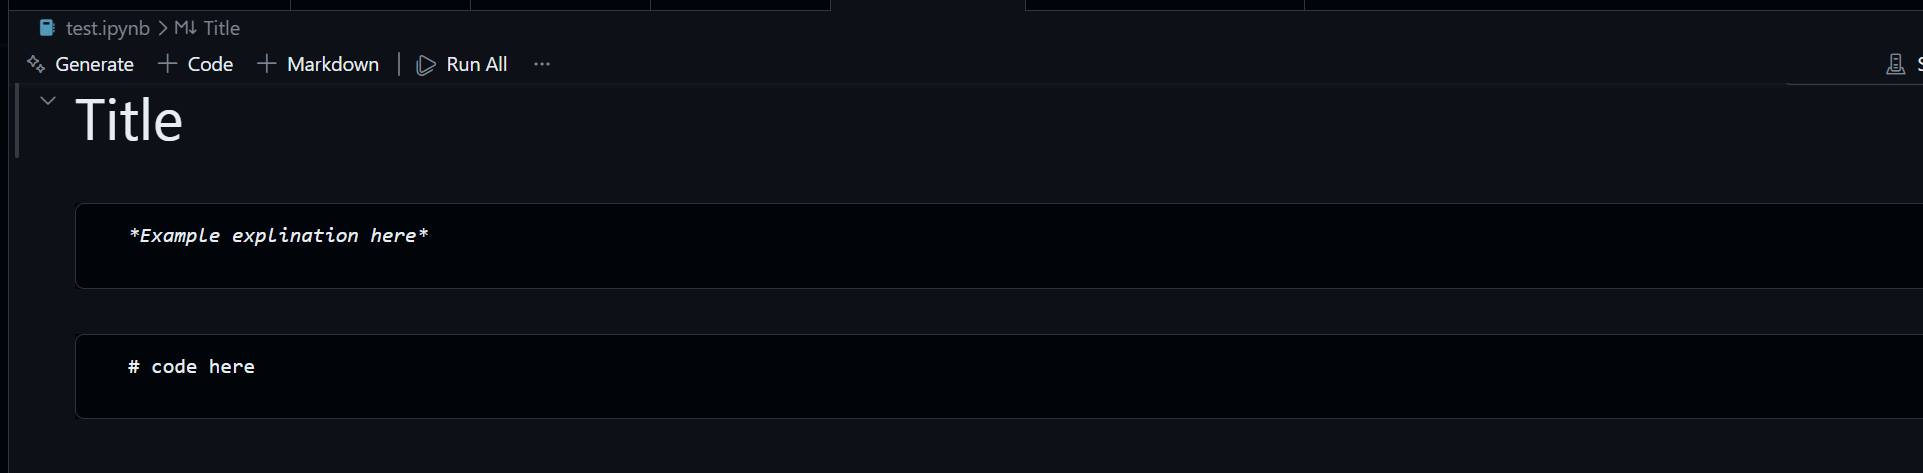
\includegraphics[keepaspectratio]{weeks/week05-polyglot-r-deepening/../../assets/images/python1/p1.png}}
\item
  \textbf{Scripts (.py):} Best for reusable utilities and automation.

  \pandocbounded{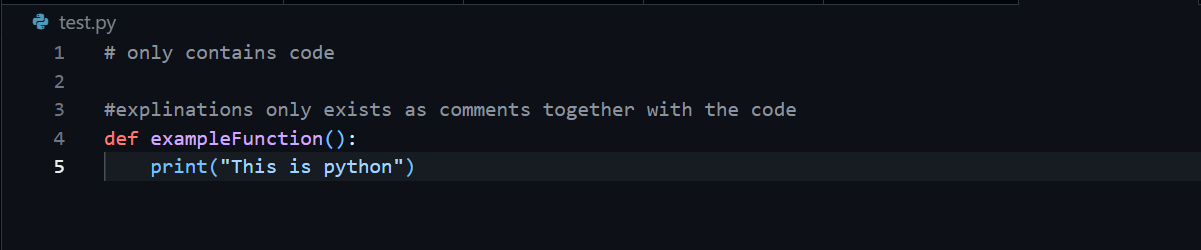
\includegraphics[keepaspectratio]{weeks/week05-polyglot-r-deepening/../../assets/images/python1/p2.png}}
\end{itemize}

\chapter{Tutorial 2: Setting Up Your Python
Environment}\label{tutorial-2-setting-up-your-python-environment}

\section{Creating Your First
Notebook}\label{creating-your-first-notebook}

Follow these steps to set up your environment in your GitHub Codespace:

\begin{enumerate}
\def\labelenumi{\arabic{enumi}.}
\item
  \textbf{New File:} In the VS Code Explorer, click the \textbf{New
  File} icon and name it \texttt{translation.ipynb}.

  \pandocbounded{
\includegraphics[keepaspectratio]{weeks/week05-polyglot-r-deepening/../../assets/images/python2/p1.png}}

  \pandocbounded{
\includegraphics[keepaspectratio]{weeks/week05-polyglot-r-deepening/../../assets/images/python2/p2.png}}
\item
  \textbf{Select Kernel:} Look at the notebook toolbar in the top right.
  Click \textbf{Select Kernel} and choose the recommended \textbf{Python
  3.x} environment.

  \pandocbounded{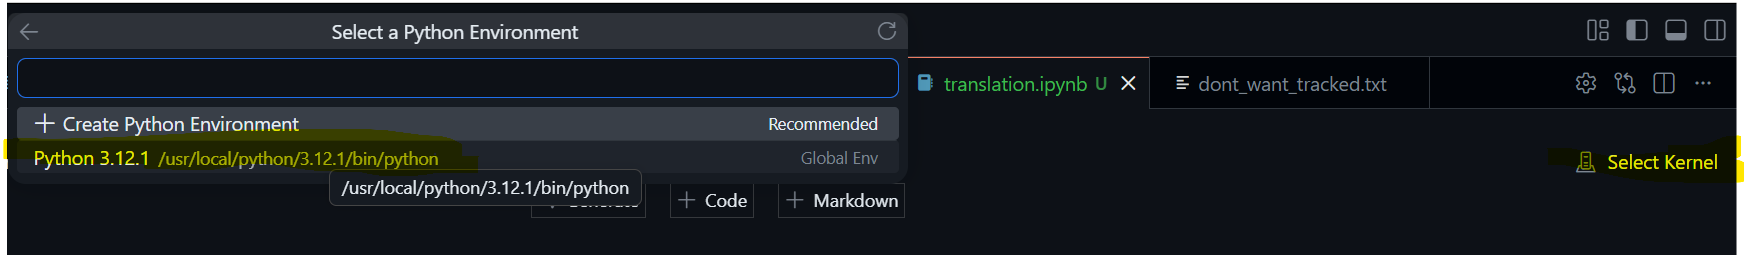
\includegraphics[keepaspectratio]{weeks/week05-polyglot-r-deepening/../../assets/images/python2/p3.png}}
\item
  \textbf{Run Code:} Build
  \texttt{print("Hello\ from\ Python!\ My\ workspace\ is\ ready.")}
  Press \textbf{Shift + Enter} to run it.

  \pandocbounded{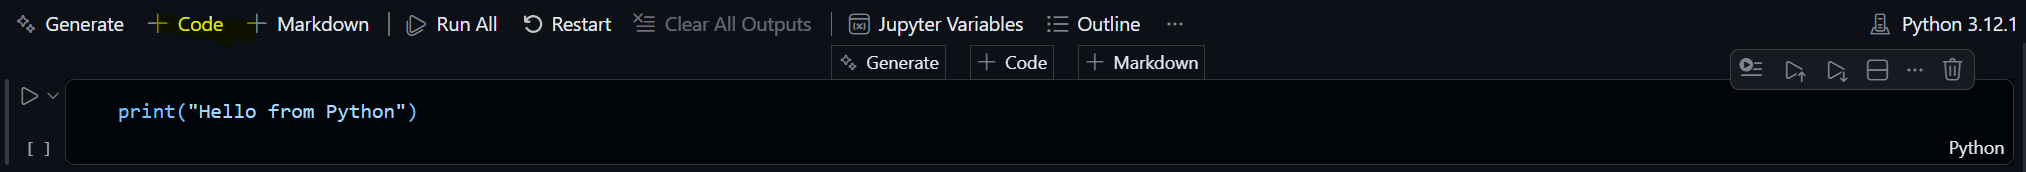
\includegraphics[keepaspectratio]{weeks/week05-polyglot-r-deepening/../../assets/images/python2/p4.png}}
\end{enumerate}

\section{The Variables Pane}\label{the-variables-pane}

Unlike RStudio, which shows variables by default, you must toggle the
view in VS Code. 1. Click the \textbf{Variables} button in the notebook
toolbar. 2. Run a cell that creates a variable (e.g.,
\texttt{age\ =\ 25}). 3. Observe \texttt{age} appearing in the pane at
the bottom.

\pandocbounded{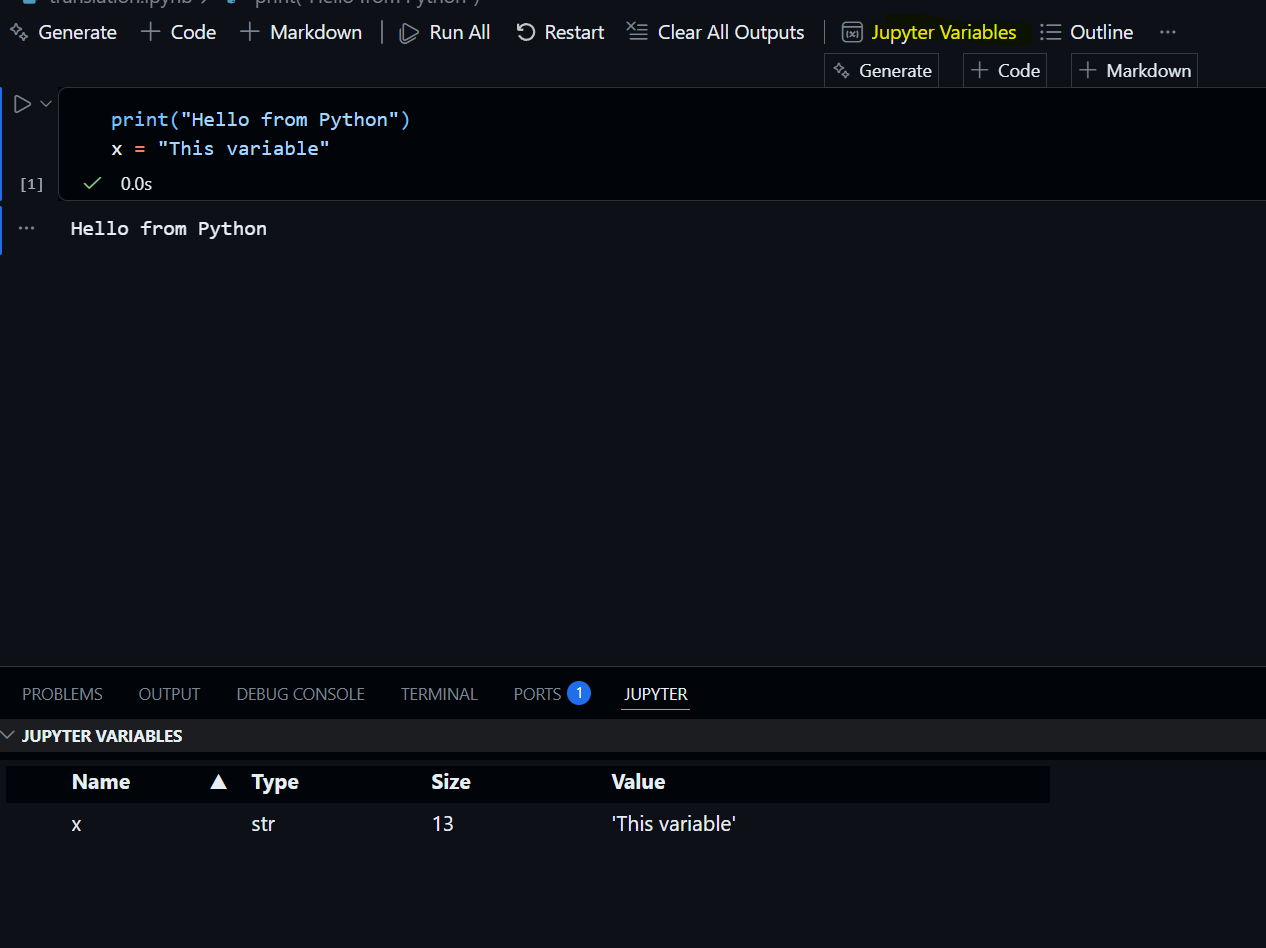
\includegraphics[keepaspectratio]{weeks/week05-polyglot-r-deepening/../../assets/images/python2/p5.png}}

\chapter{Tutorial 3: Packages and
Reproducibility}\label{tutorial-3-packages-and-reproducibility}

\section{\texorpdfstring{R \texttt{library()} vs.~Python
\texttt{import}}{R library() vs.~Python import}}\label{r-library-vs.-python-import}

In Python, we ``import'' packages and often give them nicknames
(aliases).

\begin{longtable}[]{@{}lll@{}}
\toprule\noalign{}
R & Python Equivalent & Purpose \\
\midrule\noalign{}
\endhead
\bottomrule\noalign{}
\endlastfoot
\texttt{library(dplyr)} & \texttt{import\ pandas\ as\ pd} & Data
wrangling \\
\texttt{library(ggplot2)} & \texttt{import\ seaborn\ as\ sns} &
Visualization \\
\end{longtable}

\section{\texorpdfstring{Managing
\texttt{requirements.txt}}{Managing requirements.txt}}\label{managing-requirements.txt}

Your project must be reproducible. If you use a package, you must record
it in a file called \texttt{requirements.txt}.

\begin{enumerate}
\def\labelenumi{\arabic{enumi}.}
\item
  Create a file named \texttt{requirements.txt} in your root folder.

  \pandocbounded{
\includegraphics[keepaspectratio]{weeks/week05-polyglot-r-deepening/../../assets/images/python3/p1.png}}
\item
  Add:

  \texttt{pandas==2.2.0}

  \texttt{seaborn==0.13.2}

  \pandocbounded{
\includegraphics[keepaspectratio]{weeks/week05-polyglot-r-deepening/../../assets/images/python3/p2.png}}

  Certain versions of these packages behave differently. By explicitly
  setting your versions, you can make sure you code will have
  reproducible results regardless of who is running it.
\item
  \textbf{The Rule:} Never just \texttt{pip\ install} (method on
  installing packages, which you wouldn't have to deal with in this
  class but perhaps the future) in the terminal and forget it; always
  update this file to document your steps.
\end{enumerate}

\chapter{Tutorial 4: Common Translation
Traps}\label{tutorial-4-common-translation-traps}

\section{Trap 1: The Zero-Index}\label{trap-1-the-zero-index-1}

R starts counting at \textbf{1}. Python starts counting at \textbf{0}.

\textbf{R:} \texttt{data{[}1{]}} is the first item. Note data{[}0{]}
will return nothing

\pandocbounded{
\includegraphics[keepaspectratio]{weeks/week05-polyglot-r-deepening/../../assets/images/python4/p2.png}}

\textbf{Python:} \texttt{data{[}0{]}} is the first item.

\pandocbounded{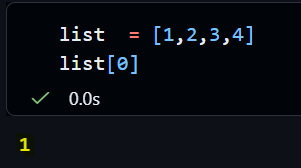
\includegraphics[keepaspectratio]{weeks/week05-polyglot-r-deepening/../../images/paste-1.png}}

\textbf{Slicing:} \texttt{df.iloc{[}0:5{]}} returns rows 0, 1, 2, 3, and
4 (5 rows total).

\section{Trap 2: Indentation}\label{trap-2-indentation}

Python uses \textbf{indentation} (spaces) instead of curly braces
\texttt{\{\}} to group code. Misaligned spaces will cause an
\texttt{IndentationError}.

\pandocbounded{
\includegraphics[keepaspectratio]{weeks/week05-polyglot-r-deepening/../../assets/images/python4/p3.png}}

\pandocbounded{
\includegraphics[keepaspectratio]{weeks/week05-polyglot-r-deepening/../../assets/images/python4/p4.png}}

\section{Trap 3: Assignment}\label{trap-3-assignment}

\begin{itemize}
\tightlist
\item
  \textbf{R:} Uses \texttt{\textless{}-} (or \texttt{=}).
\item
  \textbf{Python:} Uses \texttt{=} exclusively for assignment.
\end{itemize}

\chapter{Tutorial 5: Loading and Inspecting Health
Data}\label{tutorial-5-loading-and-inspecting-health-data}

\section{Loading Data with Pandas}\label{loading-data-with-pandas}

In your notebook, use the following code to load your health data:

\begin{Shaded}
\begin{Highlighting}[numbers=left,,]
\ImportTok{import}\NormalTok{ pandas }\ImportTok{as}\NormalTok{ pd}
\NormalTok{data }\OperatorTok{=}\NormalTok{ pd.read\_csv(}\StringTok{"data/patients.csv"}\NormalTok{)}
\end{Highlighting}
\end{Shaded}

The code below allows you to view the dataset

\begin{Shaded}
\begin{Highlighting}[numbers=left,,]
\NormalTok{data.head()}
\end{Highlighting}
\end{Shaded}

\begin{longtable}[]{@{}llllllllllllllllllllll@{}}
\toprule\noalign{}
& day & date & state.in\_hospital.in & state.in\_hospital.out &
state.in\_hospital.todate & state.in\_hospital &
state.in\_hospital.covid & state.redzone & state.reg & state.reg.covid &
... & state.pbor.care.todate & state.pbor.care &
state.pbor.deceased.care & state.pbor.deceased.care.todate &
state.pbid.care.in & state.pbid.care.out & state.pbid.care.todate &
state.pbid.care & state.pbid.deceased.care &
state.pbid.deceased.care.todate \\
\midrule\noalign{}
\endhead
\bottomrule\noalign{}
\endlastfoot
0 & 1 & 2020-03-04 & NaN & NaN & NaN & NaN & NaN & NaN & NaN & NaN & ...
& NaN & NaN & NaN & NaN & NaN & NaN & NaN & NaN & NaN & NaN \\
1 & 2 & 2020-03-05 & NaN & NaN & NaN & NaN & NaN & NaN & NaN & NaN & ...
& NaN & NaN & NaN & NaN & NaN & NaN & NaN & NaN & NaN & NaN \\
2 & 3 & 2020-03-06 & NaN & NaN & NaN & NaN & NaN & NaN & NaN & NaN & ...
& NaN & NaN & NaN & NaN & NaN & NaN & NaN & NaN & NaN & NaN \\
3 & 4 & 2020-03-07 & NaN & NaN & NaN & NaN & NaN & NaN & NaN & NaN & ...
& NaN & NaN & NaN & NaN & NaN & NaN & NaN & NaN & NaN & NaN \\
4 & 5 & 2020-03-08 & NaN & NaN & NaN & NaN & NaN & NaN & NaN & NaN & ...
& NaN & NaN & NaN & NaN & NaN & NaN & NaN & NaN & NaN & NaN \\
\end{longtable}

\pandocbounded{
\includegraphics[keepaspectratio]{weeks/week05-polyglot-r-deepening/../../assets/images/python5/p1.png}}

\chapter{Reading Tracebacks}\label{reading-tracebacks}

\section{How to Read Errors}\label{how-to-read-errors}

Python errors (Tracebacks) display a stack of calls.

\subsection{Common Example:}\label{common-example}

\texttt{FileNotFoundError:\ {[}Errno\ 2{]}\ No\ such\ file\ or\ directory:\ \textquotesingle{}Data/patients.csv\textquotesingle{}}

\pandocbounded{
\includegraphics[keepaspectratio]{weeks/week05-polyglot-r-deepening/../../assets/images/python6/p1.png}}

The first part of the message tells you what the error is, in this case
the file was not found

\texttt{FileNotFoundError}

The second part of the error tells you what is missing

\texttt{No\ such\ file\ or\ directory:\ \textquotesingle{}Data/patients.csv\textquotesingle{}}

At the top of the trace, it tells you exactly where in your code the
error was found.

\pandocbounded{
\includegraphics[keepaspectratio]{weeks/week05-polyglot-r-deepening/../../assets/images/python6/p2.png}}

The file wasn't found. Because file paths are case-sensitive,
\texttt{Data/} is different from \texttt{data/}.

\chapter{Tutorial 7: The `One Step, One Cell' AI
Workflow}\label{tutorial-7-the-one-step-one-cell-ai-workflow}

\section{Rule 1: One Step, One Cell}\label{rule-1-one-step-one-cell-1}

Don't ask the AI for a giant analysis script at once. Ask for
\textbf{one atomic step} (load, then filter, then summarize). Run and
verify each cell before moving on.

First ask AI to load

\pandocbounded{
\includegraphics[keepaspectratio]{weeks/week05-polyglot-r-deepening/../../assets/images/python7/p1.png}}

Then ask it to filter by some value

\pandocbounded{
\includegraphics[keepaspectratio]{weeks/week05-polyglot-r-deepening/../../assets/images/python7/p2.png}}

Then ask it to summarize

\pandocbounded{
\includegraphics[keepaspectratio]{weeks/week05-polyglot-r-deepening/../../assets/images/python7/p3.png}}

\section{Rule 2: Parity Audit}\label{rule-2-parity-audit}

Observe some of the differences between R and python below when it comes
to data wrangling.

\begin{longtable}[]{@{}lll@{}}
\toprule\noalign{}
Check & R & Python \\
\midrule\noalign{}
\endhead
\bottomrule\noalign{}
\endlastfoot
Row count & \texttt{nrow(df)} & \texttt{len(df)} \\
Column names & \texttt{names(df)} & \texttt{df.columns.tolist()} \\
Summary stats & \texttt{summary(df\$col)} &
\texttt{df{[}\textquotesingle{}col\textquotesingle{}{]}.describe()} \\
\end{longtable}

\chapter{Tutorial 8: Mixing R and
Python''}\label{tutorial-8-mixing-r-and-python}

\section{Why Interoperability?}\label{why-interoperability-1}

The R package \texttt{reticulate} lets you call Python from an R
session. This is perfect when you need a Python-only package but want to
keep your analysis in R.

First define the package as seen below

\pandocbounded{
\includegraphics[keepaspectratio]{weeks/week05-polyglot-r-deepening/../../assets/images/python8/p1.png}}

Then build python code as shown

\pandocbounded{
\includegraphics[keepaspectratio]{weeks/week05-polyglot-r-deepening/../../assets/images/python8/p2.png}}

Then you are able to use the results of that python code in R! Super
cool!

\pandocbounded{
\includegraphics[keepaspectratio]{weeks/week05-polyglot-r-deepening/../../assets/images/python8/p3.png}}

\subsection{Demo (Run in R)}\label{demo-run-in-r}

\begin{Shaded}
\begin{Highlighting}[numbers=left,,]
\CommentTok{\#library(reticulate) \# Run Python code inside R}
\CommentTok{\#py\_run\_string("import pandas as pd; df = pd.read\_csv(\textquotesingle{}data/patients.csv\textquotesingle{})")}
\end{Highlighting}
\end{Shaded}

Access that Python object as an R object

\begin{Shaded}
\begin{Highlighting}[numbers=left,,]
\CommentTok{\#py\_df \textless{}{-} py$df}
\CommentTok{\#head(py\_df)}
\end{Highlighting}
\end{Shaded}

\chapter{Tutorial 9: Creating Reusable Python
Scripts}\label{tutorial-9-creating-reusable-python-scripts}

\section{When to Use a Script}\label{when-to-use-a-script}

Use a \texttt{.py} script for reusable functions (like data cleaning)
that you want to use across different notebooks.

\begin{enumerate}
\def\labelenumi{\arabic{enumi}.}
\item
  Create a new file: \texttt{helpers.py}.
\item
  Add a cleaning function:

\begin{Shaded}
\begin{Highlighting}[numbers=left,,]
  \CommentTok{\# \# weeks/week05{-}polyglot{-}r{-}deepening/helpers.py}
  \CommentTok{\# from pathlib import Path}
  \CommentTok{\# import pandas as pd}
  \CommentTok{\# }
  \CommentTok{\# def load\_and\_preview(path, n=5):}
  \CommentTok{\#     p = Path(path)}
  \CommentTok{\#     if not p.exists():}
  \CommentTok{\#         raise FileNotFoundError(f"Could not find file: \{p.resolve()\}")}
  \CommentTok{\#     df = pd.read\_csv(p)}
  \CommentTok{\#     print(df.head(n))}
  \CommentTok{\#     return df}
\end{Highlighting}
\end{Shaded}
\item
  \textbf{Import it} in your notebook:

\begin{Shaded}
\begin{Highlighting}[numbers=left,,]
\CommentTok{\# from helpers import load\_and\_preview}
\CommentTok{\# load\_and\_preview("data/patients.csv")}
\end{Highlighting}
\end{Shaded}
\end{enumerate}

\chapter{Tutorial 10: Tracking Your Progress with
Git}\label{tutorial-10-tracking-your-progress-with-git}

\section{Cleaning Your Notebooks}\label{cleaning-your-notebooks}

Jupyter notebooks (\texttt{.ipynb}) store images and tables inside the
file, making Git history messy.

\textbf{Before you commit:} 1. Open the \textbf{Command Palette}
(Ctrl+Shift+P). 2. Search for \texttt{Notebook:\ Clear\ All\ Outputs}.
3. Stage and commit your changes with a professional message.

\pandocbounded{
\includegraphics[keepaspectratio]{weeks/week05-polyglot-r-deepening/../../assets/images/python10/p1.png}}

\chapter{Tutorial 11: Term Project Milestone
1}\label{tutorial-11-term-project-milestone-1}

\section{Submission Checklist}\label{submission-checklist}

Your proposal is due this Friday. Ensure it includes:

- \textbf{Research Question:} A focused health data question.

- \textbf{Data Source:} A confirmed dataset (NHANES, Kaggle, etc.).

- \textbf{Feasibility Check:} Can you load and preview the data in a
Codespace?

\textbf{Pro-Tip:} Load your dataset in \textbf{both} R and Python now to
ensure there are no surprises later in the term.

\chapter{Tutorial 12: Python Knowledge
Check}\label{tutorial-12-python-knowledge-check}

Answer these in a new Markdown cell in your notebook:

1. Why does \texttt{my\_list{[}1{]}} in Python return the \emph{second}
element?

2. What is \texttt{requirements.txt} and why is it essential for
reproducibility?

3. Why should you clear notebook outputs before committing to Git? 4.
What is the ``One Step, One Cell'' rule?

\chapter{Tutorial 13: The Bilingual Translation
Exercise}\label{tutorial-13-the-bilingual-translation-exercise}

\section{Cleaning Your Notebooks}\label{cleaning-your-notebooks-1}

\textbf{Task:} Create a Python version of your Week 3 R analysis.

1. Create \texttt{translation.ipynb}.

2. Use an LLM to translate your R steps to Python \textbf{one cell at a
time}.

\begin{enumerate}
\def\labelenumi{\arabic{enumi}.}
\setcounter{enumi}{2}
\tightlist
\item
  After each cell, verify output using the \textbf{Data Viewer}. 4.
  Extract one function into \texttt{helpers.py}. 5. Clear outputs and
  commit to Git.
\end{enumerate}

\chapter{Tutorial 14: R to Python Cheat
Sheet}\label{tutorial-14-r-to-python-cheat-sheet}

\begin{longtable}[]{@{}
  >{\raggedright\arraybackslash}p{(\linewidth - 4\tabcolsep) * \real{0.3333}}
  >{\raggedright\arraybackslash}p{(\linewidth - 4\tabcolsep) * \real{0.3333}}
  >{\raggedright\arraybackslash}p{(\linewidth - 4\tabcolsep) * \real{0.3333}}@{}}
\toprule\noalign{}
\begin{minipage}[b]{\linewidth}\raggedright
Task
\end{minipage} & \begin{minipage}[b]{\linewidth}\raggedright
R
\end{minipage} & \begin{minipage}[b]{\linewidth}\raggedright
Python
\end{minipage} \\
\midrule\noalign{}
\endhead
\bottomrule\noalign{}
\endlastfoot
Load Library & \texttt{library(dplyr)} &
\texttt{import\ pandas\ as\ pd} \\
Load CSV & \texttt{read.csv("data/f.csv")} &
\texttt{pd.read\_csv("data/f.csv")} \\
Row Count & \texttt{nrow(df)} & \texttt{len(df)} \\
Filter & \texttt{filter(df,\ age\ \textgreater{}\ 65)} &
\texttt{df{[}df{[}\textquotesingle{}age\textquotesingle{}{]}\ \textgreater{}\ 65{]}} \\
New Column & \texttt{mutate(df,\ bmi\ =\ w/h\^{}2)} &
\texttt{df{[}\textquotesingle{}bmi\textquotesingle{}{]}\ =\ df{[}\textquotesingle{}w\textquotesingle{}{]}\ /\ df{[}\textquotesingle{}h\textquotesingle{}{]}**2} \\
Summary & \texttt{summary(df\$col)} &
\texttt{df{[}\textquotesingle{}col\textquotesingle{}{]}.describe()} \\
\end{longtable}

\part{Week 6: Data Visualization}

\chapter*{Visual Storytelling}\label{visual-storytelling}
\addcontentsline{toc}{chapter}{Visual Storytelling}

\markboth{Visual Storytelling}{Visual Storytelling}

\section*{Overview}\label{overview-6}
\addcontentsline{toc}{section}{Overview}

\markright{Overview}

This chapter challenges students to move beyond default charts and
create publication-quality visualizations. You will use AI tools to
generate initial code for complex plots in ggplot2 or plotly, and then
apply human judgment to refine them for clarity, accuracy, and
aesthetics. The lesson emphasizes detecting misleading AI-generated
visuals and ``steering'' the code to tell a truthful and compelling data
story.

\section*{TODO Before Release}\label{todo-before-release-2}
\addcontentsline{toc}{section}{TODO Before Release}

\markright{TODO Before Release}

\begin{tcolorbox}[enhanced jigsaw, colframe=quarto-callout-warning-color-frame, toptitle=1mm, colback=white, leftrule=.75mm, toprule=.15mm, colbacktitle=quarto-callout-warning-color!10!white, breakable, bottomrule=.15mm, opacityback=0, title=\textcolor{quarto-callout-warning-color}{\faExclamationTriangle}\hspace{0.5em}{Content TODO}, rightrule=.15mm, bottomtitle=1mm, opacitybacktitle=0.6, titlerule=0mm, arc=.35mm, left=2mm, coltitle=black]

\begin{itemize}
\tightlist
\item
  Add a worked ggplot2 example using the shared NHANES data.
\item
  Add one intentionally misleading AI-generated chart for students to
  audit.
\item
  Add a plotly or interactive chart extension.
\item
  Add Assignment 5 instructions in
  \texttt{assignments/assignment05-visualization/}.
\item
  Add expected captions and accessibility checks for figures.
\end{itemize}

\end{tcolorbox}

\section*{Definition of Done}\label{definition-of-done-1}
\addcontentsline{toc}{section}{Definition of Done}

\markright{Definition of Done}

\begin{itemize}
\tightlist
\item
  Students can generate, critique, revise, and caption at least one
  health data visualization.
\item
  The activity includes a concrete visual audit checklist.
\item
  All example plots render in a fresh Codespace.
\end{itemize}

\chapter*{Activity: AI Visual Audit}\label{activity-ai-visual-audit}
\addcontentsline{toc}{chapter}{Activity: AI Visual Audit}

\markboth{Activity: AI Visual Audit}{Activity: AI Visual Audit}

\section*{Goal}\label{goal-1}
\addcontentsline{toc}{section}{Goal}

\markright{Goal}

Students evaluate AI-generated visualizations for correctness, clarity,
bias, aggregation choices, and misleading design.

\section*{TODO Before Release}\label{todo-before-release-3}
\addcontentsline{toc}{section}{TODO Before Release}

\markright{TODO Before Release}

\begin{tcolorbox}[enhanced jigsaw, colframe=quarto-callout-warning-color-frame, toptitle=1mm, colback=white, leftrule=.75mm, toprule=.15mm, colbacktitle=quarto-callout-warning-color!10!white, breakable, bottomrule=.15mm, opacityback=0, title=\textcolor{quarto-callout-warning-color}{\faExclamationTriangle}\hspace{0.5em}{Content TODO}, rightrule=.15mm, bottomtitle=1mm, opacitybacktitle=0.6, titlerule=0mm, arc=.35mm, left=2mm, coltitle=black]

\begin{itemize}
\tightlist
\item
  Add a starter dataset and prompt.
\item
  Add one flawed AI-generated plot and one corrected version.
\item
  Add a short answer template for students to identify what changed and
  why.
\end{itemize}

\end{tcolorbox}

\section*{Student Output}\label{student-output}
\addcontentsline{toc}{section}{Student Output}

\markright{Student Output}

\begin{itemize}
\tightlist
\item
  One original AI-generated plot.
\item
  One revised plot.
\item
  A short audit note explaining at least three changes.
\end{itemize}

\part{Week 7: EDA, Table 1 \& AI Auditing}

\chapter*{Exploring Data}\label{exploring-data}
\addcontentsline{toc}{chapter}{Exploring Data}

\markboth{Exploring Data}{Exploring Data}

\section*{Overview}\label{overview-7}
\addcontentsline{toc}{section}{Overview}

\markright{Overview}

Before modeling, you must understand your data. This chapter guides
students through the rigorous process of Exploratory Data Analysis (EDA)
and the creation of the standard ``Table 1'' for demographic
characteristics. You will learn to document every cleaning decision and
exclusion criteria in a reproducible Quarto log, ensuring that your path
from raw data to analysis dataset is transparent and repeatable by
anyone.

\section*{TODO Before Release}\label{todo-before-release-4}
\addcontentsline{toc}{section}{TODO Before Release}

\markright{TODO Before Release}

\begin{tcolorbox}[enhanced jigsaw, colframe=quarto-callout-warning-color-frame, toptitle=1mm, colback=white, leftrule=.75mm, toprule=.15mm, colbacktitle=quarto-callout-warning-color!10!white, breakable, bottomrule=.15mm, opacityback=0, title=\textcolor{quarto-callout-warning-color}{\faExclamationTriangle}\hspace{0.5em}{Content TODO}, rightrule=.15mm, bottomtitle=1mm, opacitybacktitle=0.6, titlerule=0mm, arc=.35mm, left=2mm, coltitle=black]

\begin{itemize}
\tightlist
\item
  Build a worked EDA using the NHANES example files in
  \texttt{examples/data/}.
\item
  Add Table 1 expectations and an example table.
\item
  Add a planted-error AI audit exercise.
\item
  Add Assignment 6 instructions in
  \texttt{assignments/assignment06-eda-ai-audit/}.
\item
  Connect the activity to Milestone 2 preliminary analysis.
\end{itemize}

\end{tcolorbox}

\section*{Definition of Done}\label{definition-of-done-2}
\addcontentsline{toc}{section}{Definition of Done}

\markright{Definition of Done}

\begin{itemize}
\tightlist
\item
  Students can document cleaning decisions from raw or starter data to
  an analysis-ready table.
\item
  The planted-error exercise has an instructor key.
\item
  The EDA renders without manual intervention.
\end{itemize}

\chapter*{Activity: Table 1 and AI
Audit}\label{activity-table-1-and-ai-audit}
\addcontentsline{toc}{chapter}{Activity: Table 1 and AI Audit}

\markboth{Activity: Table 1 and AI Audit}{Activity: Table 1 and AI
Audit}

\section*{Goal}\label{goal-2}
\addcontentsline{toc}{section}{Goal}

\markright{Goal}

Students create a descriptive summary and audit AI-generated code or
interpretation for planted errors.

\section*{TODO Before Release}\label{todo-before-release-5}
\addcontentsline{toc}{section}{TODO Before Release}

\markright{TODO Before Release}

\begin{tcolorbox}[enhanced jigsaw, colframe=quarto-callout-warning-color-frame, toptitle=1mm, colback=white, leftrule=.75mm, toprule=.15mm, colbacktitle=quarto-callout-warning-color!10!white, breakable, bottomrule=.15mm, opacityback=0, title=\textcolor{quarto-callout-warning-color}{\faExclamationTriangle}\hspace{0.5em}{Content TODO}, rightrule=.15mm, bottomtitle=1mm, opacitybacktitle=0.6, titlerule=0mm, arc=.35mm, left=2mm, coltitle=black]

\begin{itemize}
\tightlist
\item
  Add the starter data path.
\item
  Add the expected Table 1 variables.
\item
  Add planted errors in code, summary text, and at least one
  visualization.
\item
  Add an answer key for instructors or TAs outside the student-facing
  page.
\end{itemize}

\end{tcolorbox}

\section*{Student Output}\label{student-output-1}
\addcontentsline{toc}{section}{Student Output}

\markright{Student Output}

\begin{itemize}
\tightlist
\item
  A rendered Quarto EDA note.
\item
  A Table 1 or equivalent descriptive summary.
\item
  A written audit note listing detected errors and fixes.
\end{itemize}

\part{Week 8: Dashboard Prototypes for KT}

\chapter*{Interactive Dashboards}\label{interactive-dashboards}
\addcontentsline{toc}{chapter}{Interactive Dashboards}

\markboth{Interactive Dashboards}{Interactive Dashboards}

\section*{Overview}\label{overview-8}
\addcontentsline{toc}{section}{Overview}

\markright{Overview}

Static PDF reports often sit unread, so this chapter introduces dynamic
Knowledge Translation through Shiny apps and dashboards. Students will
take their prior EDA results and transform them into interactive web
tools that allow users to filter and explore the data themselves. You
will learn the best practices of user interface design for health data
and deploy your first live dashboard to the web via GitHub Pages or
Shinylive.

\section*{TODO Before Release}\label{todo-before-release-6}
\addcontentsline{toc}{section}{TODO Before Release}

\markright{TODO Before Release}

\begin{tcolorbox}[enhanced jigsaw, colframe=quarto-callout-warning-color-frame, toptitle=1mm, colback=white, leftrule=.75mm, toprule=.15mm, colbacktitle=quarto-callout-warning-color!10!white, breakable, bottomrule=.15mm, opacityback=0, title=\textcolor{quarto-callout-warning-color}{\faExclamationTriangle}\hspace{0.5em}{Content TODO}, rightrule=.15mm, bottomtitle=1mm, opacitybacktitle=0.6, titlerule=0mm, arc=.35mm, left=2mm, coltitle=black]

\begin{itemize}
\tightlist
\item
  Decide the required core pathway: Quarto dashboard, Shiny, or static
  HTML/JS.
\item
  Add a minimal dashboard starter with one filter, one chart, and one
  plain-language interpretation.
\item
  Add testing instructions for Codespaces.
\item
  Add Assignment 7 instructions in
  \texttt{assignments/assignment07-dashboard/}.
\item
  Add guidance for privacy-safe dashboard publishing.
\end{itemize}

\end{tcolorbox}

\section*{Definition of Done}\label{definition-of-done-3}
\addcontentsline{toc}{section}{Definition of Done}

\markright{Definition of Done}

\begin{itemize}
\tightlist
\item
  Students can produce a small dashboard-style KT artifact from prior
  EDA outputs.
\item
  The dashboard runs or renders in the supported workflow.
\item
  The page distinguishes required core work from optional deployment
  extensions.
\end{itemize}

\chapter*{Starter Dashboard}\label{starter-dashboard}
\addcontentsline{toc}{chapter}{Starter Dashboard}

\markboth{Starter Dashboard}{Starter Dashboard}

\section*{Goal}\label{goal-3}
\addcontentsline{toc}{section}{Goal}

\markright{Goal}

Students adapt a minimal dashboard-style knowledge translation product.

\section*{TODO Before Release}\label{todo-before-release-7}
\addcontentsline{toc}{section}{TODO Before Release}

\markright{TODO Before Release}

\begin{tcolorbox}[enhanced jigsaw, colframe=quarto-callout-warning-color-frame, toptitle=1mm, colback=white, leftrule=.75mm, toprule=.15mm, colbacktitle=quarto-callout-warning-color!10!white, breakable, bottomrule=.15mm, opacityback=0, title=\textcolor{quarto-callout-warning-color}{\faExclamationTriangle}\hspace{0.5em}{Content TODO}, rightrule=.15mm, bottomtitle=1mm, opacitybacktitle=0.6, titlerule=0mm, arc=.35mm, left=2mm, coltitle=black]

\begin{itemize}
\tightlist
\item
  Add the starter dashboard code.
\item
  Add a screenshot or rendered preview.
\item
  Add a fallback static version for students who cannot deploy.
\item
  Add a checklist for audience, filter labels, chart captions, and
  limitations.
\end{itemize}

\end{tcolorbox}

\section*{Required Elements}\label{required-elements}
\addcontentsline{toc}{section}{Required Elements}

\markright{Required Elements}

\begin{itemize}
\tightlist
\item
  One audience-specific question.
\item
  One interactive or dashboard-style control.
\item
  One visualization.
\item
  One plain-language interpretation.
\item
  One limitation or caution.
\end{itemize}

\part{Week 9: Communication of Scientific Findings}

\chapter*{Dynamic Presentations}\label{dynamic-presentations}
\addcontentsline{toc}{chapter}{Dynamic Presentations}

\markboth{Dynamic Presentations}{Dynamic Presentations}

\section*{Overview}\label{overview-9}
\addcontentsline{toc}{section}{Overview}

\markright{Overview}

Data analysis is useless if it cannot be understood by key stakeholders.
This chapter focuses on ``Audience-Specific KT,'' teaching you to
convert technical findings into plain language summaries and engaging
slide decks using Quarto. You will practice peer review and learn to use
LLMs to simplify jargon without losing scientific accuracy, ensuring
your work can impact policy and practice.

\section*{TODO Before Release}\label{todo-before-release-8}
\addcontentsline{toc}{section}{TODO Before Release}

\markright{TODO Before Release}

\begin{tcolorbox}[enhanced jigsaw, colframe=quarto-callout-warning-color-frame, toptitle=1mm, colback=white, leftrule=.75mm, toprule=.15mm, colbacktitle=quarto-callout-warning-color!10!white, breakable, bottomrule=.15mm, opacityback=0, title=\textcolor{quarto-callout-warning-color}{\faExclamationTriangle}\hspace{0.5em}{Content TODO}, rightrule=.15mm, bottomtitle=1mm, opacitybacktitle=0.6, titlerule=0mm, arc=.35mm, left=2mm, coltitle=black]

\begin{itemize}
\tightlist
\item
  Add a revealjs starter deck.
\item
  Add a plain-language summary exercise.
\item
  Add a peer feedback template.
\item
  Add Assignment 8 instructions in
  \texttt{assignments/assignment08-communication/}.
\item
  Add slide accessibility and citation expectations.
\end{itemize}

\end{tcolorbox}

\section*{Definition of Done}\label{definition-of-done-4}
\addcontentsline{toc}{section}{Definition of Done}

\markright{Definition of Done}

\begin{itemize}
\tightlist
\item
  Students can render a short Quarto slide deck.
\item
  Each slide has one clear purpose.
\item
  Peer feedback checks clarity, evidence, limitations, and KT value.
\end{itemize}

\chapter*{Revealjs and Peer Feedback}\label{revealjs-and-peer-feedback}
\addcontentsline{toc}{chapter}{Revealjs and Peer Feedback}

\markboth{Revealjs and Peer Feedback}{Revealjs and Peer Feedback}

\section*{Goal}\label{goal-4}
\addcontentsline{toc}{section}{Goal}

\markright{Goal}

Students turn analysis outputs into a short scientific communication
product and practice structured peer feedback.

\section*{TODO Before Release}\label{todo-before-release-9}
\addcontentsline{toc}{section}{TODO Before Release}

\markright{TODO Before Release}

\begin{tcolorbox}[enhanced jigsaw, colframe=quarto-callout-warning-color-frame, toptitle=1mm, colback=white, leftrule=.75mm, toprule=.15mm, colbacktitle=quarto-callout-warning-color!10!white, breakable, bottomrule=.15mm, opacityback=0, title=\textcolor{quarto-callout-warning-color}{\faExclamationTriangle}\hspace{0.5em}{Content TODO}, rightrule=.15mm, bottomtitle=1mm, opacitybacktitle=0.6, titlerule=0mm, arc=.35mm, left=2mm, coltitle=black]

\begin{itemize}
\tightlist
\item
  Add a minimal \texttt{format:\ revealjs} YAML example.
\item
  Add a three-slide starter structure.
\item
  Add a peer feedback form.
\end{itemize}

\end{tcolorbox}

\section*{Peer Feedback Prompts}\label{peer-feedback-prompts}
\addcontentsline{toc}{section}{Peer Feedback Prompts}

\markright{Peer Feedback Prompts}

\begin{itemize}
\tightlist
\item
  What is the main message?
\item
  What evidence supports it?
\item
  What is unclear or overclaimed?
\item
  What would improve reproducibility or audience fit?
\end{itemize}

\part{Week 10: Writing \& Publishing Reports}

\chapter*{Reproducible Reporting}\label{reproducible-reporting}
\addcontentsline{toc}{chapter}{Reproducible Reporting}

\markboth{Reproducible Reporting}{Reproducible Reporting}

\section*{Overview}\label{overview-10}
\addcontentsline{toc}{section}{Overview}

\markright{Overview}

This chapter simulates the final stretch of a research project: writing
the manuscript. Students learn to assemble their analysis, code, and
writing into a single ``dynamic report'' that automatically updates
numbers and figures if the data changes. You will explore advanced
publishing workflows to create professional, citation-ready portfolios
that demonstrate your ability to execute end-to-end data science.

\section*{TODO Before Release}\label{todo-before-release-10}
\addcontentsline{toc}{section}{TODO Before Release}

\markright{TODO Before Release}

\begin{tcolorbox}[enhanced jigsaw, colframe=quarto-callout-warning-color-frame, toptitle=1mm, colback=white, leftrule=.75mm, toprule=.15mm, colbacktitle=quarto-callout-warning-color!10!white, breakable, bottomrule=.15mm, opacityback=0, title=\textcolor{quarto-callout-warning-color}{\faExclamationTriangle}\hspace{0.5em}{Content TODO}, rightrule=.15mm, bottomtitle=1mm, opacitybacktitle=0.6, titlerule=0mm, arc=.35mm, left=2mm, coltitle=black]

\begin{itemize}
\tightlist
\item
  Add a report skeleton with sections for question, data, methods,
  findings, limitations, and AI-use note.
\item
  Add citation examples using \texttt{references.bib}.
\item
  Add GitHub Pages setup screenshots or a private submission
  alternative.
\item
  Add Assignment 9 instructions in
  \texttt{assignments/assignment09-reporting/}.
\item
  Add a citation and grounding audit.
\end{itemize}

\end{tcolorbox}

\section*{Definition of Done}\label{definition-of-done-5}
\addcontentsline{toc}{section}{Definition of Done}

\markright{Definition of Done}

\begin{itemize}
\tightlist
\item
  The report renders from source.
\item
  Citations resolve.
\item
  Outputs are regenerated by code rather than pasted manually.
\item
  The README explains how to reproduce the report.
\end{itemize}

\chapter*{Report Template}\label{report-template}
\addcontentsline{toc}{chapter}{Report Template}

\markboth{Report Template}{Report Template}

\section*{TODO Before Release}\label{todo-before-release-11}
\addcontentsline{toc}{section}{TODO Before Release}

\markright{TODO Before Release}

\begin{tcolorbox}[enhanced jigsaw, colframe=quarto-callout-warning-color-frame, toptitle=1mm, colback=white, leftrule=.75mm, toprule=.15mm, colbacktitle=quarto-callout-warning-color!10!white, breakable, bottomrule=.15mm, opacityback=0, title=\textcolor{quarto-callout-warning-color}{\faExclamationTriangle}\hspace{0.5em}{Content TODO}, rightrule=.15mm, bottomtitle=1mm, opacitybacktitle=0.6, titlerule=0mm, arc=.35mm, left=2mm, coltitle=black]

\begin{itemize}
\tightlist
\item
  Convert this into a copyable Quarto report starter.
\item
  Add bibliography setup instructions.
\item
  Add a small example table and figure.
\item
  Add an AI-use note template.
\end{itemize}

\end{tcolorbox}

\section*{Suggested Sections}\label{suggested-sections}
\addcontentsline{toc}{section}{Suggested Sections}

\markright{Suggested Sections}

\begin{itemize}
\tightlist
\item
  Research or KT question
\item
  Data source and stewardship notes
\item
  Methods and reproducibility notes
\item
  Results
\item
  Limitations
\item
  Plain-language summary
\item
  AI-use and audit note
\end{itemize}

\part{Week 11: Portfolio Surgery}

\chapter*{Advanced Topics}\label{advanced-topics}
\addcontentsline{toc}{chapter}{Advanced Topics}

\markboth{Advanced Topics}{Advanced Topics}

\section*{Overview}\label{overview-11}
\addcontentsline{toc}{section}{Overview}

\markright{Overview}

Before the final submission, students must ``bulletproof'' their work.
This chapter focuses on advanced project hygiene, dependency management
(ensuring your code runs on someone else's machine), and auditability.
You will act as a peer reviewer to identify reproducibility failures in
others' code, fixing broken paths and missing seeds, to ensure your
final project stands up to scientific scrutiny.

\section*{TODO Before Release}\label{todo-before-release-12}
\addcontentsline{toc}{section}{TODO Before Release}

\markright{TODO Before Release}

\begin{tcolorbox}[enhanced jigsaw, colframe=quarto-callout-warning-color-frame, toptitle=1mm, colback=white, leftrule=.75mm, toprule=.15mm, colbacktitle=quarto-callout-warning-color!10!white, breakable, bottomrule=.15mm, opacityback=0, title=\textcolor{quarto-callout-warning-color}{\faExclamationTriangle}\hspace{0.5em}{Content TODO}, rightrule=.15mm, bottomtitle=1mm, opacitybacktitle=0.6, titlerule=0mm, arc=.35mm, left=2mm, coltitle=black]

\begin{itemize}
\tightlist
\item
  Add a fresh Codespace stress-test protocol.
\item
  Add a broken-project debugging exercise.
\item
  Add Assignment 10 instructions in
  \texttt{assignments/assignment10-portfolio-surgery/}.
\item
  Add Milestone 4 peer review instructions.
\item
  Add a final portfolio readiness checklist.
\end{itemize}

\end{tcolorbox}

\section*{Definition of Done}\label{definition-of-done-6}
\addcontentsline{toc}{section}{Definition of Done}

\markright{Definition of Done}

\begin{itemize}
\tightlist
\item
  A peer can clone or open the repository in a fresh Codespace and
  reproduce the core outputs.
\item
  Broken paths, missing dependencies, unclear READMEs, and ungrounded AI
  claims are fixed.
\item
  The final portfolio checklist is linked from this page.
\end{itemize}

\chapter*{Reproducibility Stress
Test}\label{reproducibility-stress-test}
\addcontentsline{toc}{chapter}{Reproducibility Stress Test}

\markboth{Reproducibility Stress Test}{Reproducibility Stress Test}

\section*{Goal}\label{goal-5}
\addcontentsline{toc}{section}{Goal}

\markright{Goal}

Students test whether a project can run in a fresh environment and
document every failure before final submission.

\section*{TODO Before Release}\label{todo-before-release-13}
\addcontentsline{toc}{section}{TODO Before Release}

\markright{TODO Before Release}

\begin{tcolorbox}[enhanced jigsaw, colframe=quarto-callout-warning-color-frame, toptitle=1mm, colback=white, leftrule=.75mm, toprule=.15mm, colbacktitle=quarto-callout-warning-color!10!white, breakable, bottomrule=.15mm, opacityback=0, title=\textcolor{quarto-callout-warning-color}{\faExclamationTriangle}\hspace{0.5em}{Content TODO}, rightrule=.15mm, bottomtitle=1mm, opacitybacktitle=0.6, titlerule=0mm, arc=.35mm, left=2mm, coltitle=black]

\begin{itemize}
\tightlist
\item
  Add step-by-step fresh Codespace test instructions.
\item
  Add a failure log template.
\item
  Add peer review roles and timing.
\item
  Add final repair checklist.
\end{itemize}

\end{tcolorbox}

\section*{Failure Log Template}\label{failure-log-template}
\addcontentsline{toc}{section}{Failure Log Template}

\markright{Failure Log Template}

\begin{longtable}[]{@{}llll@{}}
\toprule\noalign{}
Check & Result & Fix needed & Owner \\
\midrule\noalign{}
\endhead
\bottomrule\noalign{}
\endlastfoot
Repository opens in fresh Codespace & & & \\
Packages install or restore & & & \\
Report renders & & & \\
Dashboard runs or renders & & & \\
README instructions are accurate & & & \\
\end{longtable}

\part{Weeks 12-13: Project Presentations}

\chapter*{Week 12: Term Project Presentations, Part
1}\label{week-12-term-project-presentations-part-1}
\addcontentsline{toc}{chapter}{Week 12: Term Project Presentations, Part
1}

\markboth{Week 12: Term Project Presentations, Part 1}{Week 12: Term
Project Presentations, Part 1}

\section*{Overview}\label{overview-12}
\addcontentsline{toc}{section}{Overview}

\markright{Overview}

This session is the first presentation block for Milestone 5. Students
present their portfolio work with an emphasis on scientific clarity,
knowledge translation, reproducibility, and auditability.

\section*{TODO Before Release}\label{todo-before-release-14}
\addcontentsline{toc}{section}{TODO Before Release}

\markright{TODO Before Release}

\begin{tcolorbox}[enhanced jigsaw, colframe=quarto-callout-warning-color-frame, toptitle=1mm, colback=white, leftrule=.75mm, toprule=.15mm, colbacktitle=quarto-callout-warning-color!10!white, breakable, bottomrule=.15mm, opacityback=0, title=\textcolor{quarto-callout-warning-color}{\faExclamationTriangle}\hspace{0.5em}{Content TODO}, rightrule=.15mm, bottomtitle=1mm, opacitybacktitle=0.6, titlerule=0mm, arc=.35mm, left=2mm, coltitle=black]

\begin{itemize}
\tightlist
\item
  Add final presentation timing rules.
\item
  Add slide submission instructions.
\item
  Add the peer feedback form or link.
\item
  Add the presentation rubric from \texttt{milestones/m5-presentation/}.
\end{itemize}

\end{tcolorbox}

\section*{Definition of Done}\label{definition-of-done-7}
\addcontentsline{toc}{section}{Definition of Done}

\markright{Definition of Done}

\begin{itemize}
\tightlist
\item
  Slides render before class.
\item
  The project repository link is available to reviewers.
\item
  The presenter can explain the dataset, workflow, major findings,
  limitations, and AI-use audit trail.
\end{itemize}

\chapter*{Week 13: Term Project Presentations, Part
2}\label{week-13-term-project-presentations-part-2}
\addcontentsline{toc}{chapter}{Week 13: Term Project Presentations, Part
2}

\markboth{Week 13: Term Project Presentations, Part 2}{Week 13: Term
Project Presentations, Part 2}

\section*{Overview}\label{overview-13}
\addcontentsline{toc}{section}{Overview}

\markright{Overview}

This session completes Milestone 5 presentations and gives students a
final opportunity to collect feedback before the Final Portfolio
deadline.

\section*{TODO Before Release}\label{todo-before-release-15}
\addcontentsline{toc}{section}{TODO Before Release}

\markright{TODO Before Release}

\begin{tcolorbox}[enhanced jigsaw, colframe=quarto-callout-warning-color-frame, toptitle=1mm, colback=white, leftrule=.75mm, toprule=.15mm, colbacktitle=quarto-callout-warning-color!10!white, breakable, bottomrule=.15mm, opacityback=0, title=\textcolor{quarto-callout-warning-color}{\faExclamationTriangle}\hspace{0.5em}{Content TODO}, rightrule=.15mm, bottomtitle=1mm, opacitybacktitle=0.6, titlerule=0mm, arc=.35mm, left=2mm, coltitle=black]

\begin{itemize}
\tightlist
\item
  Confirm which groups present in Part 2.
\item
  Add final reminders for the Dec 11 portfolio submission.
\item
  Add a closing reflection prompt on reproducibility and knowledge
  translation.
\end{itemize}

\end{tcolorbox}

\section*{Definition of Done}\label{definition-of-done-8}
\addcontentsline{toc}{section}{Definition of Done}

\markright{Definition of Done}

\begin{itemize}
\tightlist
\item
  Remaining presentations are complete.
\item
  Peer feedback has been returned to presenters.
\item
  Students know exactly what must change before final portfolio
  submission.
\end{itemize}

\part{Assignments and Milestones}

\chapter*{Assignments}\label{assignments}
\addcontentsline{toc}{chapter}{Assignments}

\markboth{Assignments}{Assignments}

Weekly assignments are scaffolded practice. Assignments 1-3 are
foundational gates; Assignments 4-10 support the project portfolio and
use the best-5-of-7 grading policy described in the syllabus.

\section*{Assignment Map}\label{assignment-map}
\addcontentsline{toc}{section}{Assignment Map}

\markright{Assignment Map}

\begin{longtable}[]{@{}
  >{\raggedright\arraybackslash}p{(\linewidth - 6\tabcolsep) * \real{0.2308}}
  >{\raggedleft\arraybackslash}p{(\linewidth - 6\tabcolsep) * \real{0.3077}}
  >{\raggedright\arraybackslash}p{(\linewidth - 6\tabcolsep) * \real{0.2308}}
  >{\raggedright\arraybackslash}p{(\linewidth - 6\tabcolsep) * \real{0.2308}}@{}}
\toprule\noalign{}
\begin{minipage}[b]{\linewidth}\raggedright
Assignment
\end{minipage} & \begin{minipage}[b]{\linewidth}\raggedleft
Week
\end{minipage} & \begin{minipage}[b]{\linewidth}\raggedright
Focus
\end{minipage} & \begin{minipage}[b]{\linewidth}\raggedright
Template folder
\end{minipage} \\
\midrule\noalign{}
\endhead
\bottomrule\noalign{}
\endlastfoot
Assignment 1 & 2 & Codespaces, Quarto, commit/sync &
\texttt{assignments/assignment01-workflows/} \\
Assignment 2 & 3 & R with AI, tidyverse, functions, \texttt{renv} &
\texttt{assignments/assignment02-r-with-ai/} \\
Assignment 3 & 4 & Git collaboration and repo hygiene &
\texttt{assignments/assignment03-git/} \\
Assignment 4 & 5 & Polyglot awareness and R deepening &
\texttt{assignments/assignment04-polyglot/} \\
Assignment 5 & 6 & Visualization and AI visual audit &
\texttt{assignments/assignment05-visualization/} \\
Assignment 6 & 7 & EDA, Table 1, planted-error audit &
\texttt{assignments/assignment06-eda-ai-audit/} \\
Assignment 7 & 8 & Dashboard-style KT prototype &
\texttt{assignments/assignment07-dashboard/} \\
Assignment 8 & 9 & Scientific communication and peer feedback &
\texttt{assignments/assignment08-communication/} \\
Assignment 9 & 10 & Reporting, citations, publishing &
\texttt{assignments/assignment09-reporting/} \\
Assignment 10 & 11 & Portfolio surgery and reproducibility test &
\texttt{assignments/assignment10-portfolio-surgery/} \\
\end{longtable}

\section*{TODO}\label{todo}
\addcontentsline{toc}{section}{TODO}

\markright{TODO}

\begin{tcolorbox}[enhanced jigsaw, colframe=quarto-callout-warning-color-frame, toptitle=1mm, colback=white, leftrule=.75mm, toprule=.15mm, colbacktitle=quarto-callout-warning-color!10!white, breakable, bottomrule=.15mm, opacityback=0, title=\textcolor{quarto-callout-warning-color}{\faExclamationTriangle}\hspace{0.5em}{Warning}, rightrule=.15mm, bottomtitle=1mm, opacitybacktitle=0.6, titlerule=0mm, arc=.35mm, left=2mm, coltitle=black]

Create a student-facing \texttt{README.md} in each assignment folder
from \texttt{assignments/assignment-template.qmd}.

\end{tcolorbox}

\chapter*{Assignment Template}\label{assignment-template}
\addcontentsline{toc}{chapter}{Assignment Template}

\markboth{Assignment Template}{Assignment Template}

Use this template for all weekly applied assignments.

\section*{Student-Facing Brief}\label{student-facing-brief}
\addcontentsline{toc}{section}{Student-Facing Brief}

\markright{Student-Facing Brief}

\begin{itemize}
\tightlist
\item
  \textbf{Purpose:}
\item
  \textbf{Inputs:}
\item
  \textbf{Expected output:}
\item
  \textbf{Submission location:}
\item
  \textbf{Due date:}
\end{itemize}

\section*{Required Files}\label{required-files}
\addcontentsline{toc}{section}{Required Files}

\markright{Required Files}

\begin{itemize}
\tightlist
\item
  \texttt{README.md}
\item
  One rendered Quarto output or dashboard preview.
\item
  Source \texttt{.qmd}, \texttt{.R}, \texttt{.py}, or supporting files
  needed to rerun the work.
\item
  Data files, or clear instructions for obtaining them, when
  redistribution is not allowed.
\end{itemize}

\section*{Reproducibility Contract}\label{reproducibility-contract}
\addcontentsline{toc}{section}{Reproducibility Contract}

\markright{Reproducibility Contract}

\begin{itemize}
\tightlist
\item
  The work runs in a fresh GitHub Codespace.
\item
  Paths are relative to the project root.
\item
  Required packages are declared.
\item
  Outputs can be regenerated without manual editing.
\item
  AI-generated code or text is audited and documented.
\end{itemize}

\section*{Grading Checklist}\label{grading-checklist}
\addcontentsline{toc}{section}{Grading Checklist}

\markright{Grading Checklist}

\begin{itemize}
\tightlist
\item
  Clear question or task.
\item
  Correct and reproducible code.
\item
  Evidence of verification.
\item
  Clear writing and captions.
\item
  Honest limitations and AI-use note.
\end{itemize}

\chapter*{Project Milestones}\label{project-milestones}
\addcontentsline{toc}{chapter}{Project Milestones}

\markboth{Project Milestones}{Project Milestones}

The term project is built through staged milestones so students practice
reproducibility, feedback, and knowledge translation before the final
submission.

\begin{longtable}[]{@{}
  >{\raggedright\arraybackslash}p{(\linewidth - 4\tabcolsep) * \real{0.3333}}
  >{\raggedright\arraybackslash}p{(\linewidth - 4\tabcolsep) * \real{0.3333}}
  >{\raggedright\arraybackslash}p{(\linewidth - 4\tabcolsep) * \real{0.3333}}@{}}
\toprule\noalign{}
\begin{minipage}[b]{\linewidth}\raggedright
Milestone
\end{minipage} & \begin{minipage}[b]{\linewidth}\raggedright
Due
\end{minipage} & \begin{minipage}[b]{\linewidth}\raggedright
Deliverable
\end{minipage} \\
\midrule\noalign{}
\endhead
\bottomrule\noalign{}
\endlastfoot
M0 & Week 4 Monday & Group formation and repository setup \\
M1 & Week 6 Monday & Proposal, dataset selection, provenance/stewardship
statement \\
M2 & Week 7 Monday & Preliminary analysis, Table 1 or descriptive
summary, runnable repository \\
M3 & Week 10 Monday & Draft report and dashboard-style KT product for
review \\
M4 & Week 11 Monday & Peer review with reproducibility and auditability
checks \\
M5 & Weeks 12-13 & In-class presentation \\
Final Portfolio & Dec 11 Friday & Complete reproducible portfolio \\
\end{longtable}

\section*{TODO}\label{todo-1}
\addcontentsline{toc}{section}{TODO}

\markright{TODO}

\begin{tcolorbox}[enhanced jigsaw, colframe=quarto-callout-warning-color-frame, toptitle=1mm, colback=white, leftrule=.75mm, toprule=.15mm, colbacktitle=quarto-callout-warning-color!10!white, breakable, bottomrule=.15mm, opacityback=0, title=\textcolor{quarto-callout-warning-color}{\faExclamationTriangle}\hspace{0.5em}{Warning}, rightrule=.15mm, bottomtitle=1mm, opacitybacktitle=0.6, titlerule=0mm, arc=.35mm, left=2mm, coltitle=black]

Create detailed milestone briefs in each \texttt{milestones/} subfolder
from \texttt{milestones/milestone-template.qmd}.

\end{tcolorbox}

\chapter*{Milestone Template}\label{milestone-template}
\addcontentsline{toc}{chapter}{Milestone Template}

\markboth{Milestone Template}{Milestone Template}

Use this template for project milestones M0-M5 and the Final Portfolio.

\section*{Deliverable}\label{deliverable-1}
\addcontentsline{toc}{section}{Deliverable}

\markright{Deliverable}

\begin{itemize}
\tightlist
\item
  \textbf{Milestone:}
\item
  \textbf{Due:}
\item
  \textbf{Submit:}
\item
  \textbf{Main artifact:}
\end{itemize}

\section*{Required Evidence}\label{required-evidence}
\addcontentsline{toc}{section}{Required Evidence}

\markright{Required Evidence}

\begin{itemize}
\tightlist
\item
  Repository link.
\item
  Rendered report, dashboard, slides, or review document.
\item
  Commit history showing meaningful progress.
\item
  AI-use note.
\item
  Reproducibility check result.
\end{itemize}

\section*{Definition of Done}\label{definition-of-done-9}
\addcontentsline{toc}{section}{Definition of Done}

\markright{Definition of Done}

\begin{itemize}
\tightlist
\item
  The artifact opens or renders in the supported workflow.
\item
  Data provenance and stewardship decisions are documented.
\item
  The work avoids unsupported causal or predictive claims.
\item
  A peer or TA can rerun the project from a fresh environment.
\end{itemize}

\part{Reference: Data Sources}

\chapter*{Data Source: NHIS}\label{data-source-nhis}
\addcontentsline{toc}{chapter}{Data Source: NHIS}

\markboth{Data Source: NHIS}{Data Source: NHIS}

The National Health Interview Survey (NHIS) is a cross-sectional
household interview survey conducted by the US Centers for Disease
Control (CDC). The survey collects information on the health status,
health care access, and health behaviors of the US population.

\begin{center}

\includegraphics[width=0.9\linewidth,height=\textheight,keepaspectratio]{references/data-sources/../../assets/images/data1/nhis1.png}
\end{center}

\marginnote{\begin{footnotesize}

\href{https://www.cdc.gov/nchs/nhis/index.html}{CDC website for NHIS}

\end{footnotesize}}

\subsection*{About NHIS}\label{about-nhis}
\addcontentsline{toc}{subsection}{About NHIS}

You can find more information about the NHIS survey by clicking on
\href{https://www.cdc.gov/nchs/nhis/about/index.html}{About NHIS}:

\begin{center}

\includegraphics[width=0.9\linewidth,height=\textheight,keepaspectratio]{references/data-sources/../../assets/images/data1/nhis2.png}
\end{center}

\begin{center}

\includegraphics[width=0.9\linewidth,height=\textheight,keepaspectratio]{references/data-sources/../../assets/images/data1/nhis3.png}
\end{center}

On the \texttt{About\ NHIS} page, you will find information about what
the survey collects, data and documentation, the instructions on how to
use the data, and information on related NHIS surveys.

\begin{center}
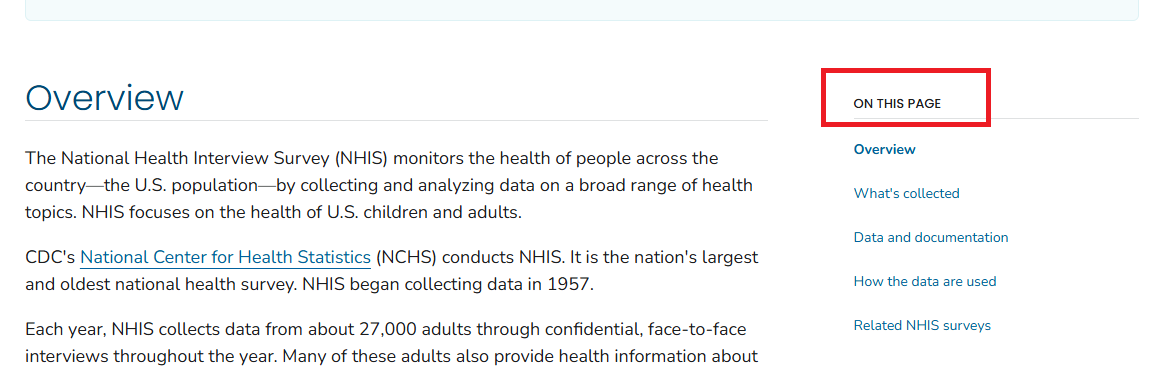
\includegraphics[width=0.9\linewidth,height=\textheight,keepaspectratio]{references/data-sources/../../assets/images/data1/nhis4.png}
\end{center}

You can click on each of the links or scroll down to find information on
each of these topics one by one. For example, if we click on the
\texttt{How\ the\ data\ are\ used} link, we will find information as
follows:

\begin{center}
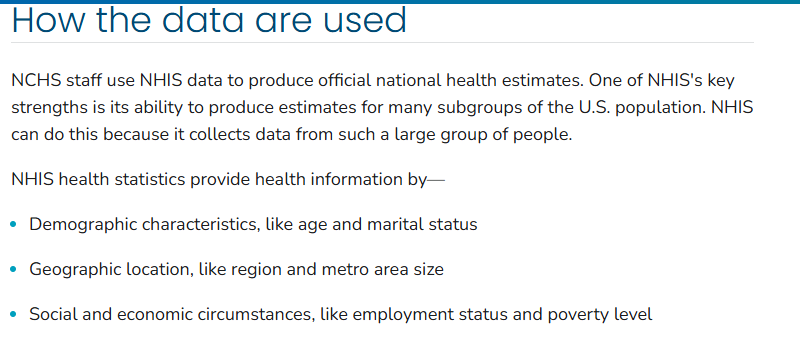
\includegraphics[width=0.9\linewidth,height=\textheight,keepaspectratio]{references/data-sources/../../assets/images/data1/nhis5.png}
\end{center}

\subsection*{About the Data}\label{about-the-data}
\addcontentsline{toc}{subsection}{About the Data}

If you click on \texttt{About\ the\ Data} link, you will find
information about the NHIS questionnaires, datasets, and documentation:

\begin{center}

\includegraphics[width=0.9\linewidth,height=\textheight,keepaspectratio]{references/data-sources/../../assets/images/data1/nhis6.png}
\end{center}

\marginnote{\begin{footnotesize}

\href{https://www.cdc.gov/nchs/nhis/documentation/index.html}{NHIS Data,
Questionnaires and Related Documentation}

\end{footnotesize}}

Under the \texttt{Overview} tab, you will find information about
different NHIS cycles and the questionnaires, datasets, and
documentation available in each cycle. As an example, let's click on the
\texttt{2023\ NHIS\ Questionnaires,\ Datasets,\ and\ Documentation} link
to see the details for the 2023 NHIS:

\begin{center}
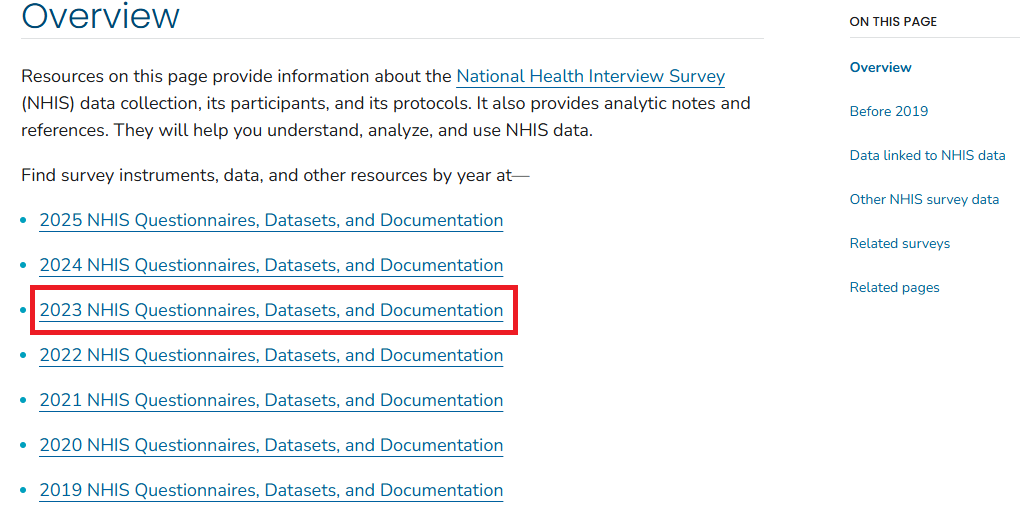
\includegraphics[width=0.9\linewidth,height=\textheight,keepaspectratio]{references/data-sources/../../assets/images/data1/nhis7.png}
\end{center}

\subsection*{NHIS Questionnaires, Datasets, and
Documentation}\label{nhis-questionnaires-datasets-and-documentation}
\addcontentsline{toc}{subsection}{NHIS Questionnaires, Datasets, and
Documentation}

To view the description of the 2023 NHIS, click on the
\texttt{Survey\ description\ document} link:

\begin{center}
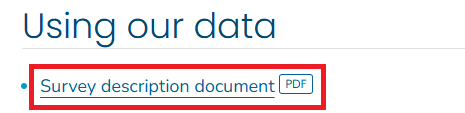
\includegraphics[width=0.9\linewidth,height=\textheight,keepaspectratio]{references/data-sources/../../assets/images/data1/nhis8.png}
\end{center}

This will open the PDF of the 2023 NHIS survey description.
Alternatively, you can right-click on the link, click on
\texttt{Save\ link\ as...} and save the PDF file on your computer for
future reference.

\begin{center}
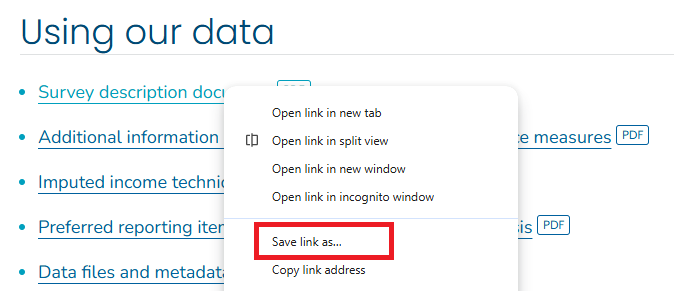
\includegraphics[width=0.9\linewidth,height=\textheight,keepaspectratio]{references/data-sources/../../assets/images/data1/nhis9.png}
\end{center}

Similarly, you can open and save the questionnaires and related
materials under the \texttt{Questionnaires\ and\ survey\ materials} tab.

\marginnote{\begin{footnotesize}

Data are available in 5 categories:

\begin{itemize}
\tightlist
\item
  Sample adult interview
\item
  Sample child interview
\item
  Parent-child pair data
\item
  Imputed income
\item
  Paradata
\end{itemize}

\end{footnotesize}}

In the recent NHIS, data are available in 5 categories: interview data
for adults, interview data for children, data for parent-child pairs,
imputed income, and paradata. You can click each link for documentation
to see a summary of the data and the codebook.

\begin{center}
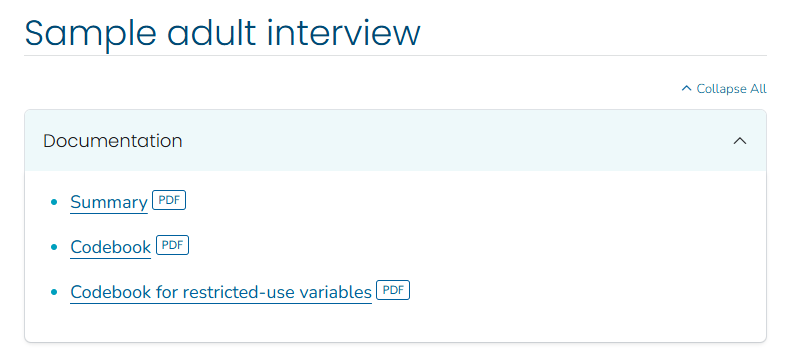
\includegraphics[width=0.9\linewidth,height=\textheight,keepaspectratio]{references/data-sources/../../assets/images/data1/nhis10.png}
\end{center}

\subsection*{NHIS Data}\label{nhis-data}
\addcontentsline{toc}{subsection}{NHIS Data}

The data files are stored on the NHIS website in different formats. You
can save the dataset in any statistical package that supports these file
formats, e.g., ASCII, CSV, SAS. Let us save the \texttt{adult} dataset
in the CSV format, which is in a zip file.

\begin{center}
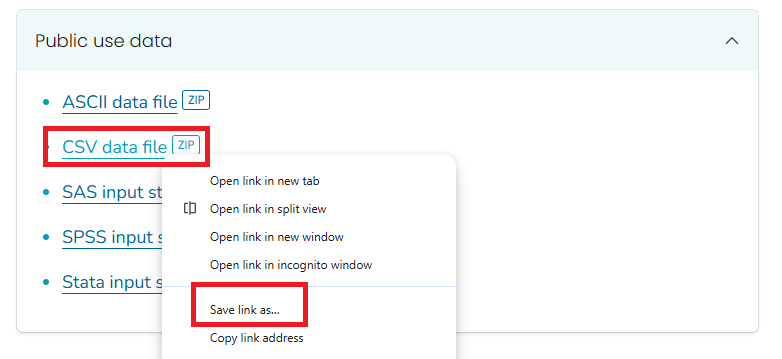
\includegraphics[width=0.9\linewidth,height=\textheight,keepaspectratio]{references/data-sources/../../assets/images/data1/nhis11.png}
\end{center}

\begin{center}
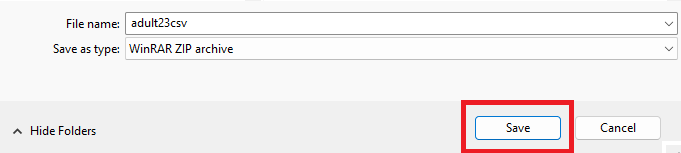
\includegraphics[width=0.9\linewidth,height=\textheight,keepaspectratio]{references/data-sources/../../assets/images/data1/nhis12.png}
\end{center}

The next step is to unzip the file to extract the CSV. Depending on your
computer, you can unzip the file with or without software. For example,
if you are using Windows, you can right-click the zip file and select
\texttt{Extract\ All...} to unzip it.

\begin{center}
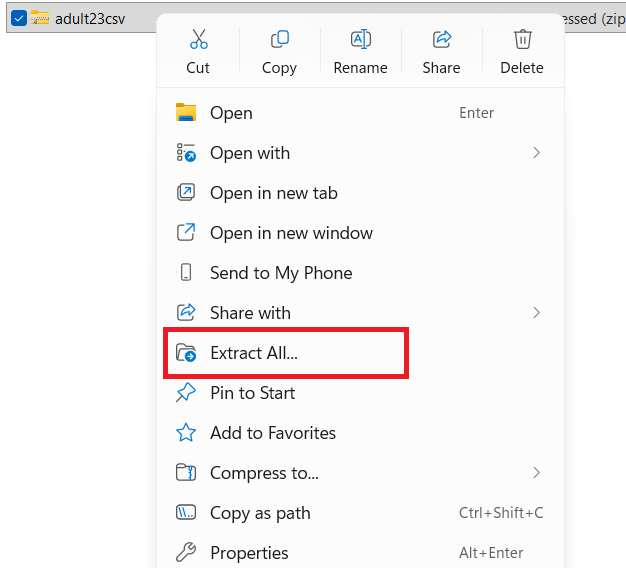
\includegraphics[width=0.9\linewidth,height=\textheight,keepaspectratio]{references/data-sources/../../assets/images/data1/nhis13.png}
\end{center}

Once unzipped, you will find two files: the CSV file for the dataset and
a readme file with some instructions. Below is the example for the
\texttt{adult} dataset:

\begin{center}
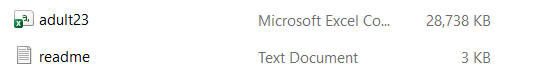
\includegraphics[width=0.9\linewidth,height=\textheight,keepaspectratio]{references/data-sources/../../assets/images/data1/nhis14.png}
\end{center}

To open the datafile in Excel, - you can double click on the CSV file,
or - right click on the CSV file and click on \texttt{Open}.

Later, you will learn how to open the data file in different statistical
software. For Excel, it would take a few seconds/minutes because of the
large size of the dataset. Once you open the data file, you will see the
data in a tabular format with rows and columns.

\begin{center}
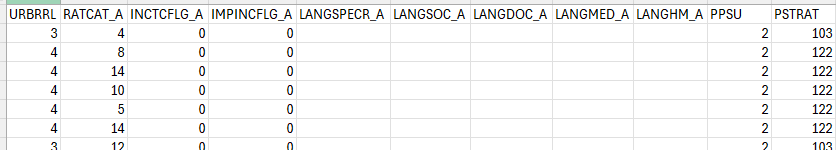
\includegraphics[width=0.9\linewidth,height=\textheight,keepaspectratio]{references/data-sources/../../assets/images/data1/nhis15.png}
\end{center}

\begin{itemize}
\tightlist
\item
  Each row represents a person.
\item
  Each column represents a variable.
\item
  The first row contains the variable names. The remaining rows contain
  the data for each person.
\end{itemize}

\subsection*{Use of the codebook}\label{use-of-the-codebook}
\addcontentsline{toc}{subsection}{Use of the codebook}

To understand the variables in the dataset, you can refer to the
codebook. The codebook provides information about the variable names,
labels, and values. For example, we want to understand the variable
\texttt{SEX\_A}:

\begin{center}
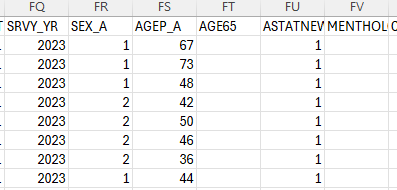
\includegraphics[width=0.9\linewidth,height=\textheight,keepaspectratio]{references/data-sources/../../assets/images/data1/nhis16.png}
\end{center}

We can look for \texttt{SEX\_A} in the codebook, which will provide us
with the variable label and the values for that variable (e.g., 1 for
Male, 2 for Female, and so on).

\begin{center}
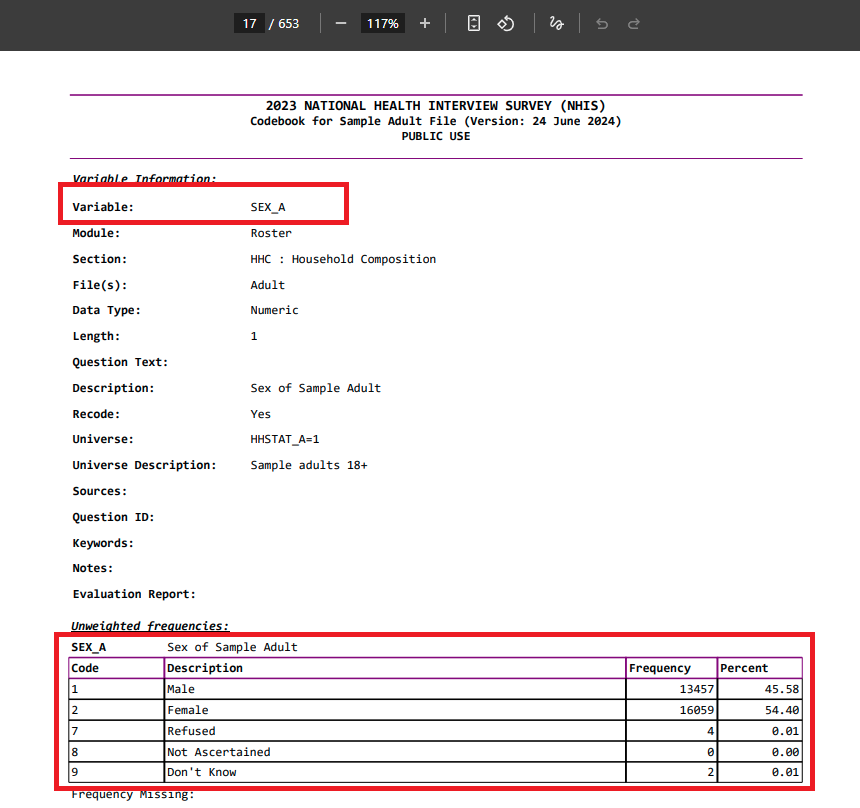
\includegraphics[width=0.9\linewidth,height=\textheight,keepaspectratio]{references/data-sources/../../assets/images/data1/nhis17.png}
\end{center}

There are so many variables in the dataset, and it is not possible to
understand all of them at once. You can refer to the codebook to
understand the variables that you are interested in for your analysis.
For example, the \texttt{WTFA\_A} variable is the sample adult weight
variable used to calculate weighted estimates for the US adult
population. Similarly, the \texttt{HYPEV\_A} variable is the
hypertension ever variable, indicating whether a doctor or other health
professional has ever told the person they have hypertension. Again, you
can refer to the codebook to understand the variables that you are
interested in.

\chapter*{Data Source: NHANES}\label{data-source-nhanes}
\addcontentsline{toc}{chapter}{Data Source: NHANES}

\markboth{Data Source: NHANES}{Data Source: NHANES}

The National Health and Nutrition Examination Survey (NHANES) is a
cross-sectional survey conducted by the US Centers for Disease Control
(CDC). The survey collects information on the health and nutritional
status of the US population. The survey includes interviews, physical
examinations, and laboratory tests.

\begin{center}

\includegraphics[width=0.9\linewidth,height=\textheight,keepaspectratio]{references/data-sources/../../assets/images/data2/nhanes1.png}
\end{center}

\marginnote{\begin{footnotesize}

\href{https://wwwn.cdc.gov/nchs/nhanes/Default.aspx}{CDC website for
NHANES}

\end{footnotesize}}

\subsection*{About NHANES}\label{about-nhanes}
\addcontentsline{toc}{subsection}{About NHANES}

You can find more information about the NHANES survey by clicking on
\href{https://www.cdc.gov/nchs/nhanes/about/}{About NHANES}:

\begin{center}

\includegraphics[width=0.9\linewidth,height=\textheight,keepaspectratio]{references/data-sources/../../assets/images/data2/nhanes2.png}
\end{center}

\begin{center}

\includegraphics[width=0.9\linewidth,height=\textheight,keepaspectratio]{references/data-sources/../../assets/images/data2/nhanes3.png}
\end{center}

On the \texttt{About\ NHANES} page, you will find information about what
the survey collects, data and documentation, the instructions on how to
use the data, and information on related NHANES surveys.

\begin{center}
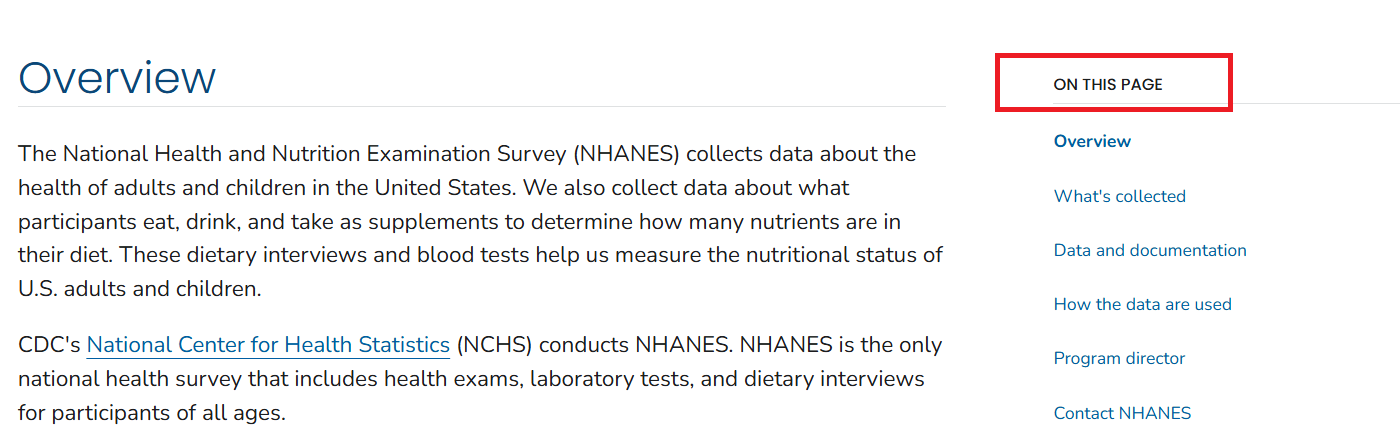
\includegraphics[width=0.9\linewidth,height=\textheight,keepaspectratio]{references/data-sources/../../assets/images/data2/nhanes4.png}
\end{center}

You can click on each of the links or scroll down to find information on
each of these topics one by one. For example, if we click on the
\texttt{Data\ and\ documentation} link, we will find information as
follows:

\begin{center}
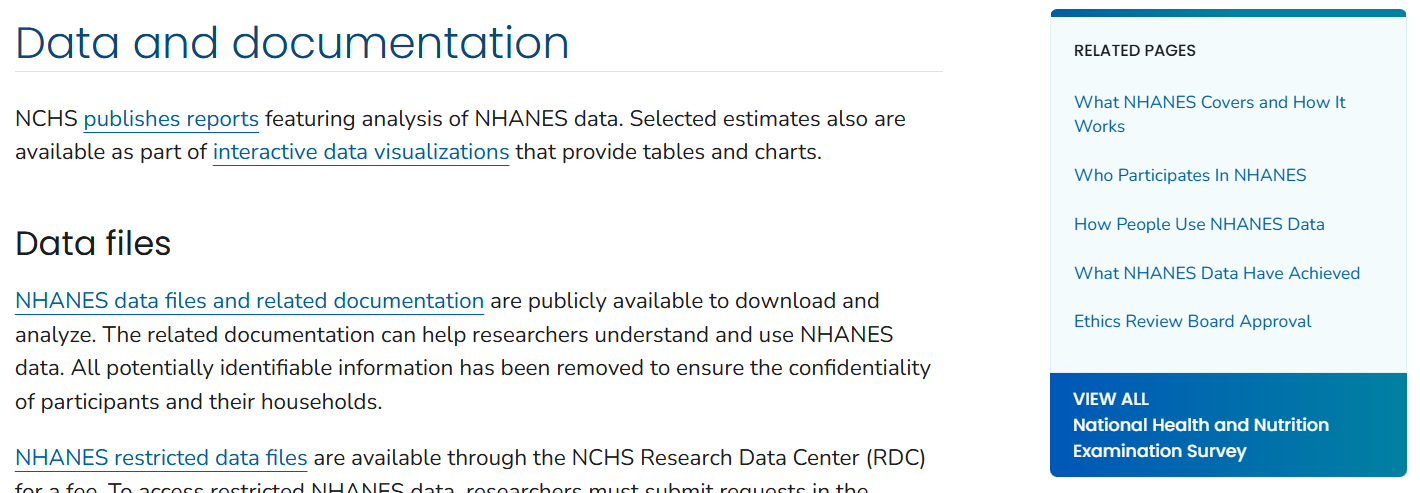
\includegraphics[width=0.9\linewidth,height=\textheight,keepaspectratio]{references/data-sources/../../assets/images/data2/nhanes5.png}
\end{center}

\subsection*{Survey Methods and Analytic
Guidelines}\label{survey-methods-and-analytic-guidelines}
\addcontentsline{toc}{subsection}{Survey Methods and Analytic
Guidelines}

If you click on
\texttt{NHANES\ data\ files\ and\ related\ documentation} link, you will
find information about the NHANES questionnaires, datasets, and
documentation:

\begin{center}
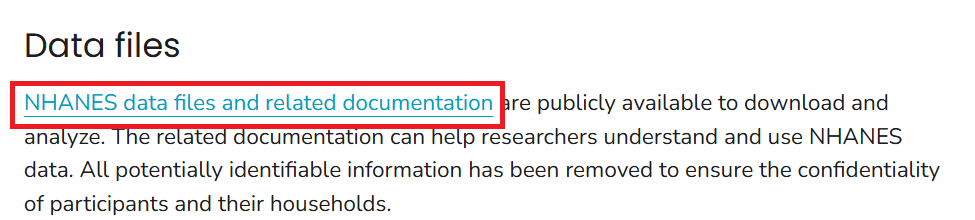
\includegraphics[width=0.9\linewidth,height=\textheight,keepaspectratio]{references/data-sources/../../assets/images/data2/nhanes6.png}
\end{center}

\begin{center}
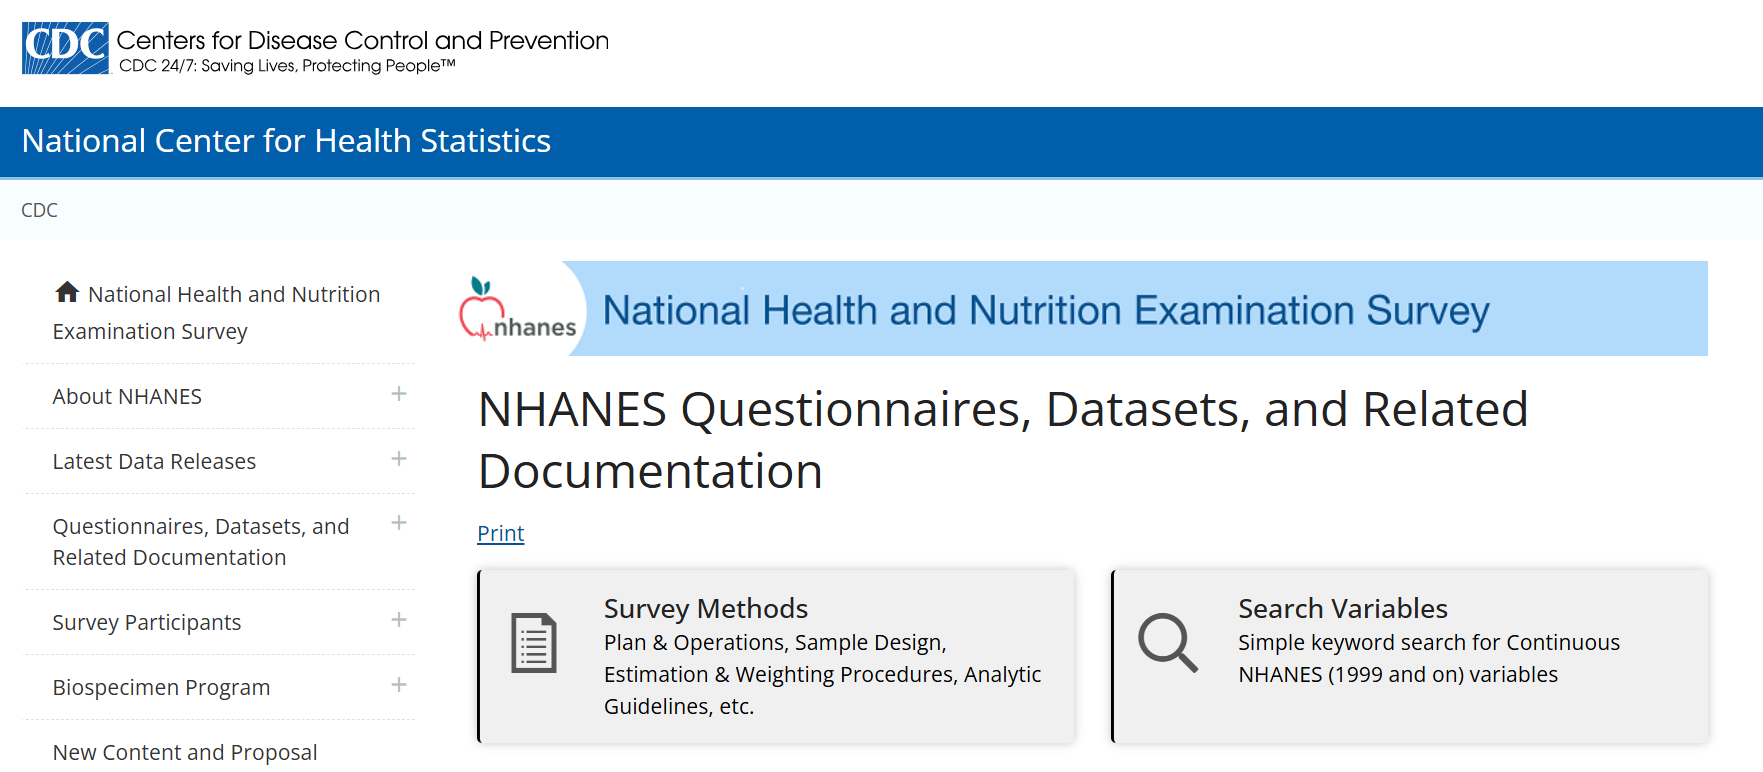
\includegraphics[width=0.9\linewidth,height=\textheight,keepaspectratio]{references/data-sources/../../assets/images/data2/nhanes7.png}
\end{center}

\marginnote{\begin{footnotesize}

\href{https://wwwn.cdc.gov/nchs/nhanes/Default.aspx}{NHANES data files
and related documentation}

\end{footnotesize}}

You can click \texttt{Survey\ Methods} to find information on survey
methods and analytic guidelines. The
\texttt{Survey\ Methods\ and\ Analytic\ Guidelines} page provides
information about the plan and operation of the NHANES survey, the
sampling design, methods for calculating weights and variance
estimation, and guidelines for analyzing NHANES data, along with links
to related resources.

\begin{center}
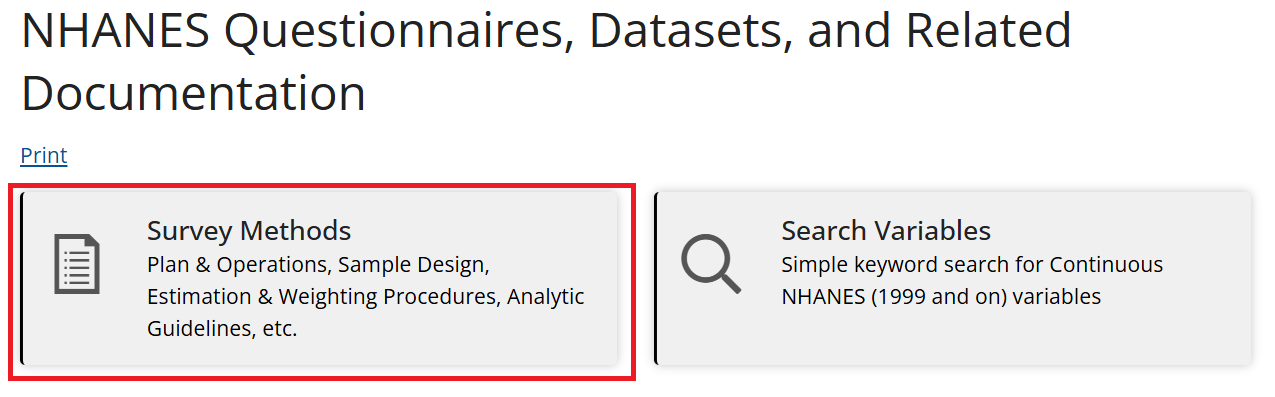
\includegraphics[width=0.9\linewidth,height=\textheight,keepaspectratio]{references/data-sources/../../assets/images/data2/nhanes8.png}
\end{center}

\subsection*{Search Variables}\label{search-variables}
\addcontentsline{toc}{subsection}{Search Variables}

If you click on \texttt{Search\ Variables} link, you will find a search
tool to search for variables in the NHANES datasets (1999 and on).

\begin{center}
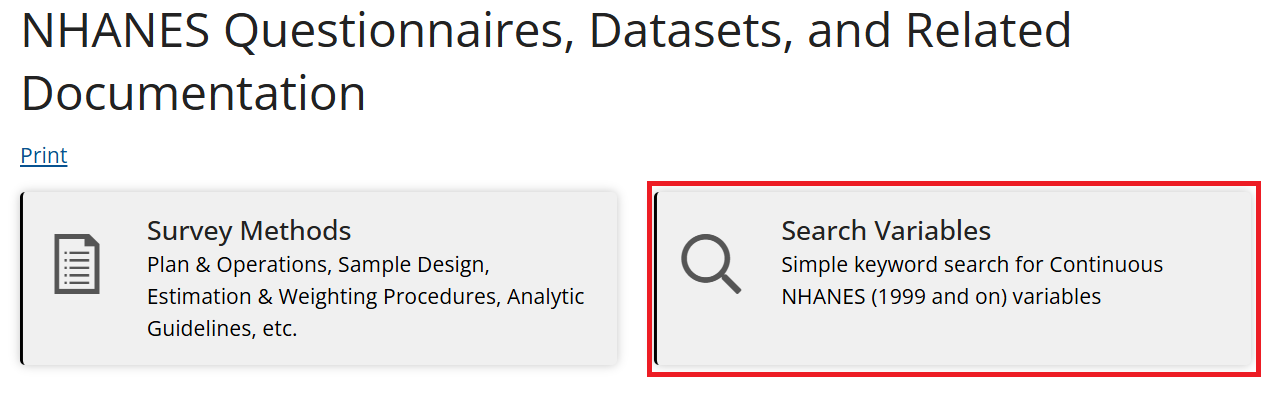
\includegraphics[width=0.9\linewidth,height=\textheight,keepaspectratio]{references/data-sources/../../assets/images/data2/nhanes9.png}
\end{center}

You can search for variables by entering keywords in the search box. For
example, if you enter \texttt{diabetes} in the search box, you will find
a list of variables related to diabetes in the NHANES datasets.

\begin{center}
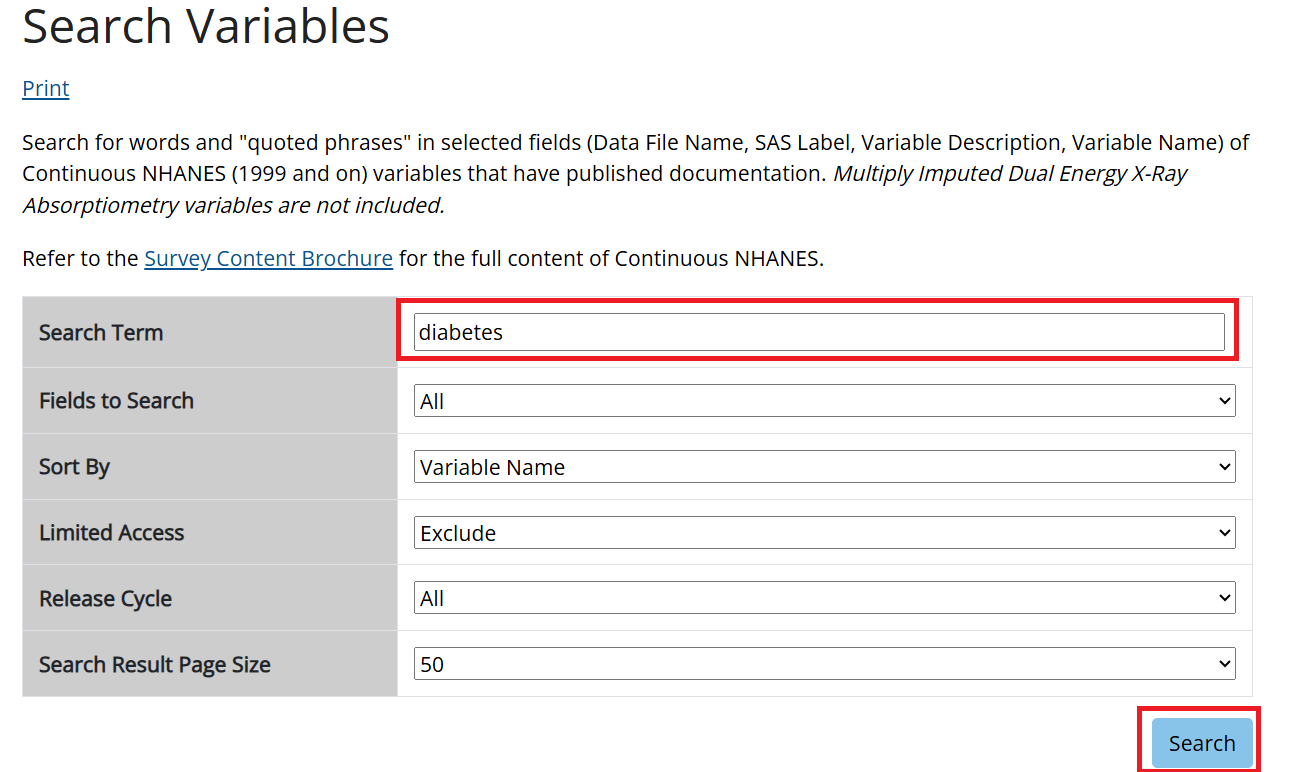
\includegraphics[width=0.9\linewidth,height=\textheight,keepaspectratio]{references/data-sources/../../assets/images/data2/nhanes10.png}
\end{center}

\begin{center}
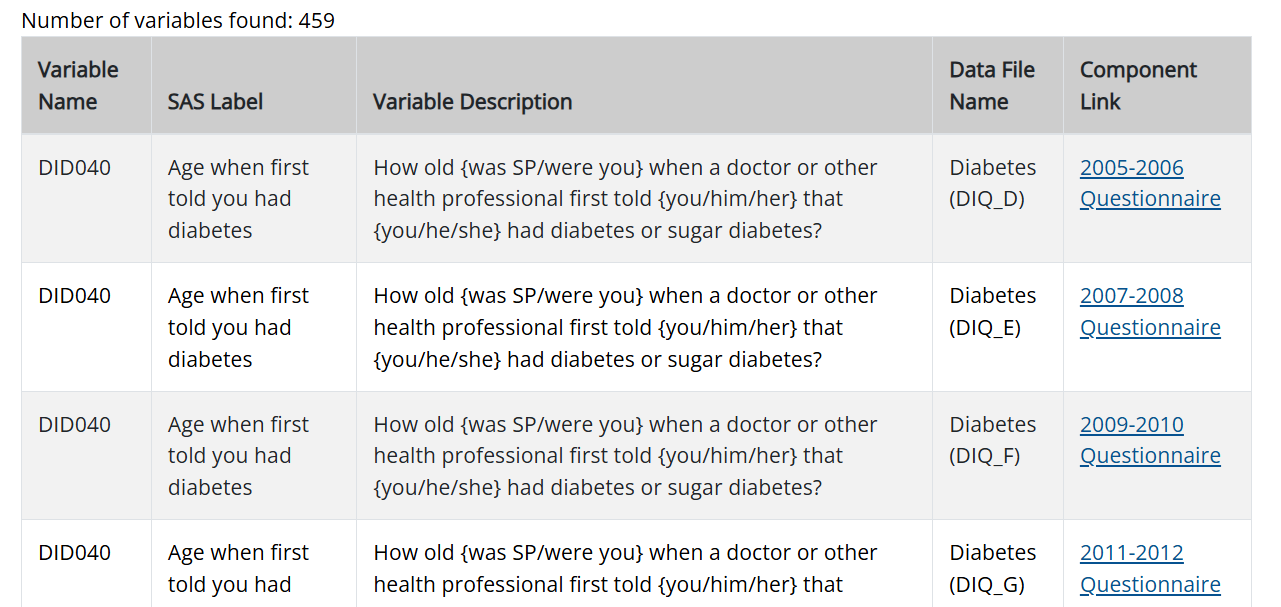
\includegraphics[width=0.9\linewidth,height=\textheight,keepaspectratio]{references/data-sources/../../assets/images/data2/nhanes11.png}
\end{center}

You can restrict your search to a specific NHANES cycle by selecting the
cycle from the drop-down menu. For example, if you select the
\texttt{2017-2018} cycle, you will find a list of variables related to
diabetes in the 2017-2018 NHANES dataset.

\begin{center}
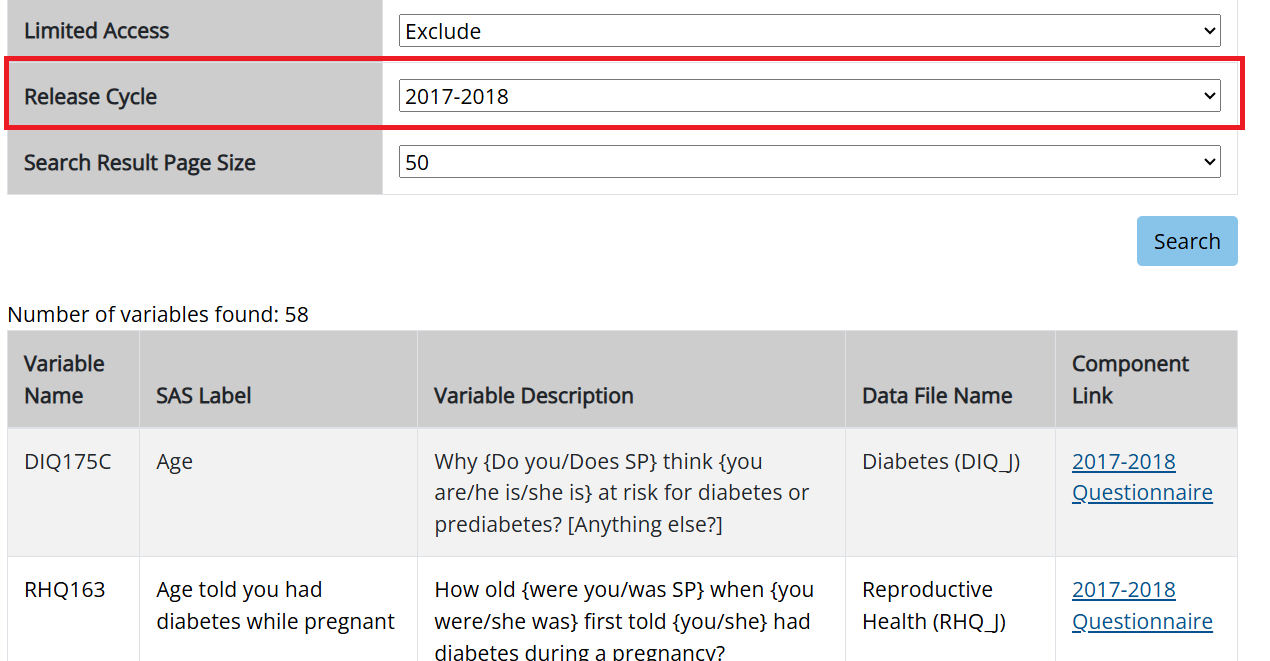
\includegraphics[width=0.9\linewidth,height=\textheight,keepaspectratio]{references/data-sources/../../assets/images/data2/nhanes12.png}
\end{center}

\subsection*{NHANES Questionnaires, Datasets, and
Documentation}\label{nhanes-questionnaires-datasets-and-documentation}
\addcontentsline{toc}{subsection}{NHANES Questionnaires, Datasets, and
Documentation}

Let's explore the questionnaires, datasets, and documentation for the
2017-2018 NHANES cycle. You need to click on \texttt{NHANES\ 2017-2018}
under the \texttt{Continuous\ NHANES} tab:

\begin{center}
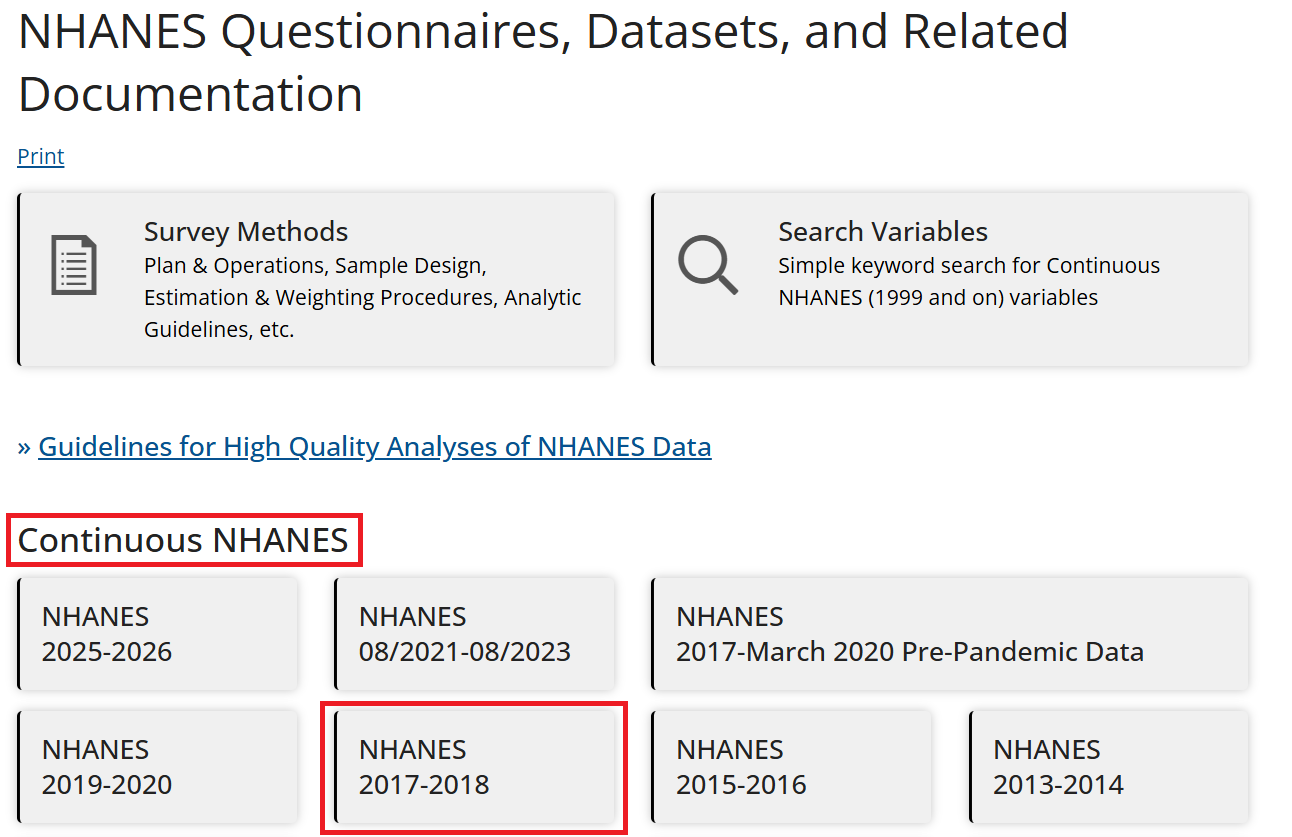
\includegraphics[width=0.9\linewidth,height=\textheight,keepaspectratio]{references/data-sources/../../assets/images/data2/nhanes13.png}
\end{center}

This will open the page for the 2017-2018 NHANES cycle, where you can
find information on the survey description, questionnaires, datasets,
and documentation.

\begin{center}
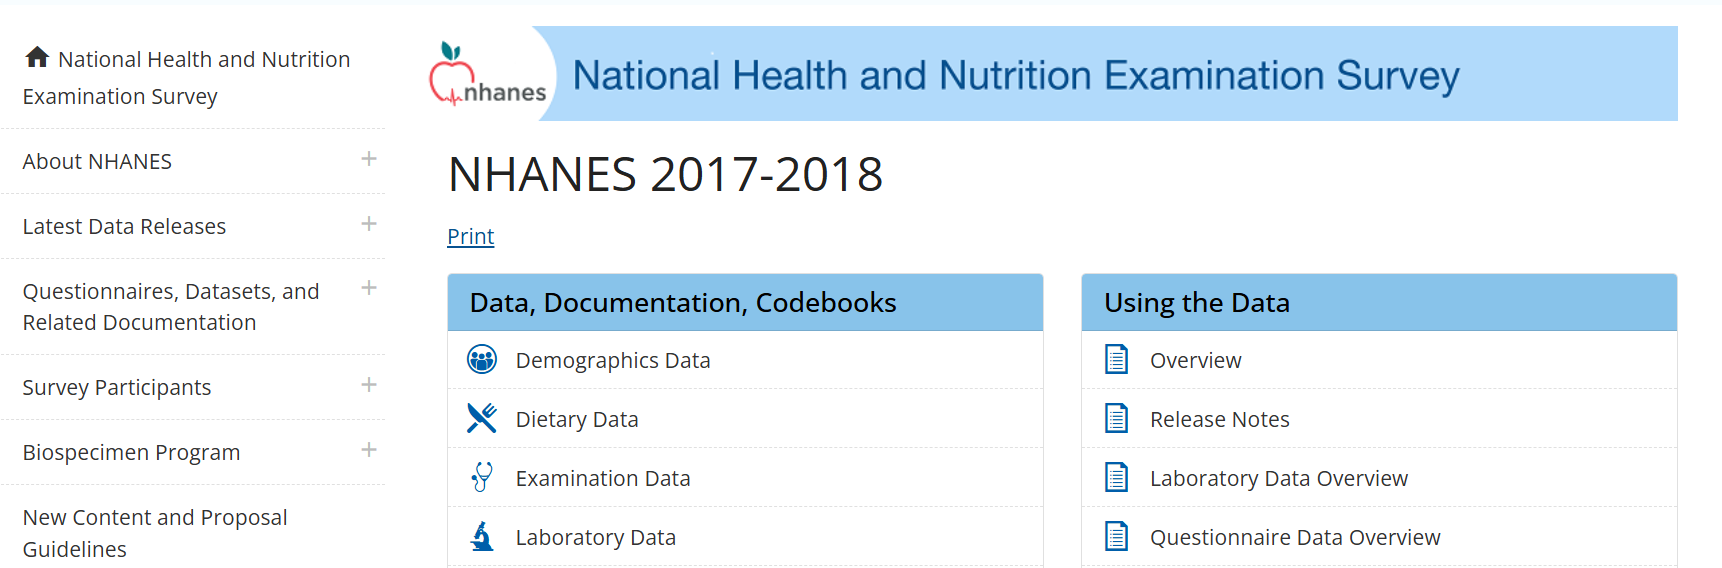
\includegraphics[width=0.9\linewidth,height=\textheight,keepaspectratio]{references/data-sources/../../assets/images/data2/nhanes14.png}
\end{center}

\marginnote{\begin{footnotesize}

Data are available in 6 categories:

\begin{itemize}
\tightlist
\item
  Demographics
\item
  Dietary
\item
  Examination
\item
  Laboratory
\item
  Questionnaire
\item
  Limited Access
\end{itemize}

\end{footnotesize}}

There are six categories of data available for the 2017-2018 NHANES
cycle: Demographics, Dietary, Examination, Laboratory, Questionnaire,
and Limited Access data. You can click each category to find the
datasets and documentation available in that category. For example, if
you click on \texttt{Demographics\ Data}, you will find a list of
datasets and documentation related to demographics data in the 2017-2018
NHANES cycle.

\begin{center}
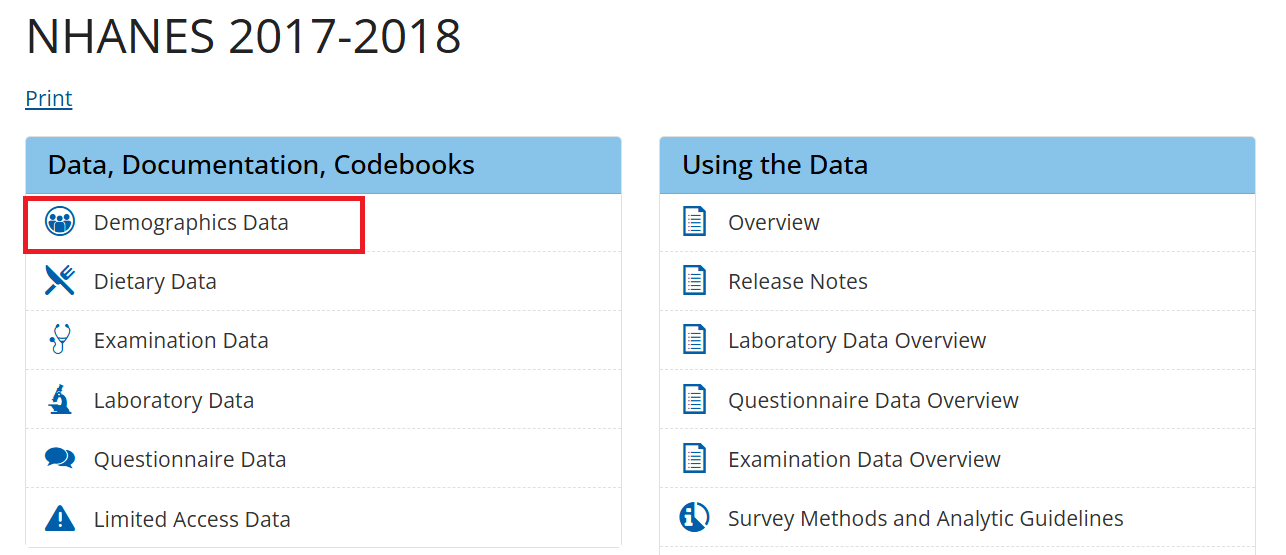
\includegraphics[width=0.9\linewidth,height=\textheight,keepaspectratio]{references/data-sources/../../assets/images/data2/nhanes15.png}
\end{center}

\begin{center}
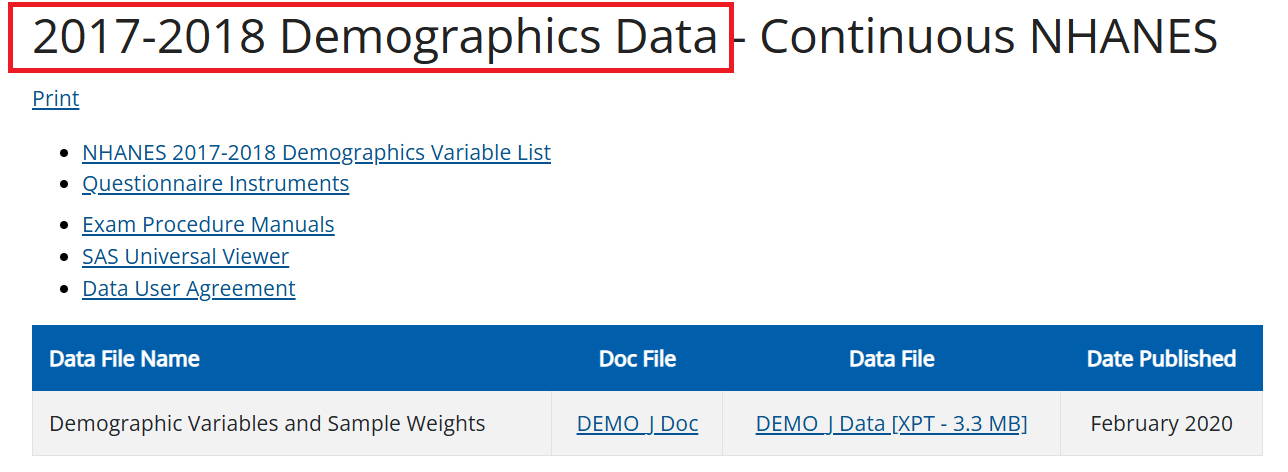
\includegraphics[width=0.9\linewidth,height=\textheight,keepaspectratio]{references/data-sources/../../assets/images/data2/nhanes16.png}
\end{center}

There is a \texttt{Doc\ File} available for each dataset that provides
information about the dataset, including the variables it contains,
their coding, and any special considerations for using it. It is
important to read the \texttt{Doc} file before using the dataset to
understand the data structure and how to use it properly. The
\texttt{Data\ File} contains the dataset data in \texttt{.XPT} format,
which is a SAS Transport file, not a CSV.

\begin{center}
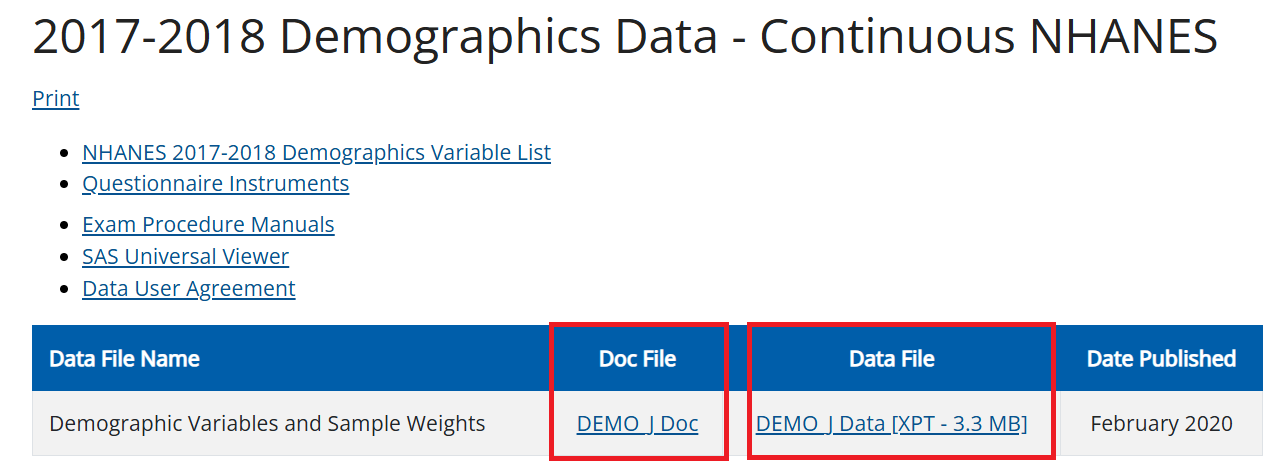
\includegraphics[width=0.9\linewidth,height=\textheight,keepaspectratio]{references/data-sources/../../assets/images/data2/nhanes17.png}
\end{center}

\subsection*{Data}\label{data}
\addcontentsline{toc}{subsection}{Data}

You need to click on the \texttt{DEMO\_J\ Data\ {[}XPT\ -\ 3.3\ MB{]}}
link to download the dataset. Note that you cannot easily open an
\texttt{.XPT} file in Excel or Google Sheets. In the real world, data
isn't always in a friendly format. For this week, let's download the
\texttt{NHANES\_Demo\_Converted.csv} file from our Canvas page to look
at the rows. Later, we will use an AI co-pilot to write R code that
reads \texttt{.XPT} files automatically.

Let's open the \texttt{NHANES\_Demo\_Converted.csv} file in Excel and
see the first few rows:

\begin{center}
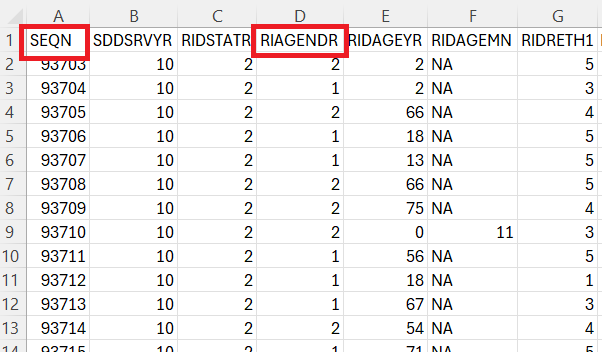
\includegraphics[width=0.9\linewidth,height=\textheight,keepaspectratio]{references/data-sources/../../assets/images/data2/nhanes18.png}
\end{center}

\begin{itemize}
\tightlist
\item
  Each row represents a person.
\item
  Each column represents a variable.
\item
  The first row contains the variable names. The remaining rows contain
  the data for each person.
\end{itemize}

For example, \texttt{SEQN} is the unique identifier for each person in
the dataset, and \texttt{RIAGENDR} is the variable for gender.

\subsection*{Use of the Codebook}\label{use-of-the-codebook-1}
\addcontentsline{toc}{subsection}{Use of the Codebook}

To understand the variables in the dataset, you can refer to the
codebook. The codebook provides information about the variable names,
labels, and values. The \texttt{Doc\ File} explained earlier contains
the codebook for the dataset. You need to click on the
\texttt{DEMO\_J\ Doc} link to open the codebook on a new page. Let's we
want to understand the variables \texttt{SEQN} and \texttt{RIAGENDR}:

\begin{center}
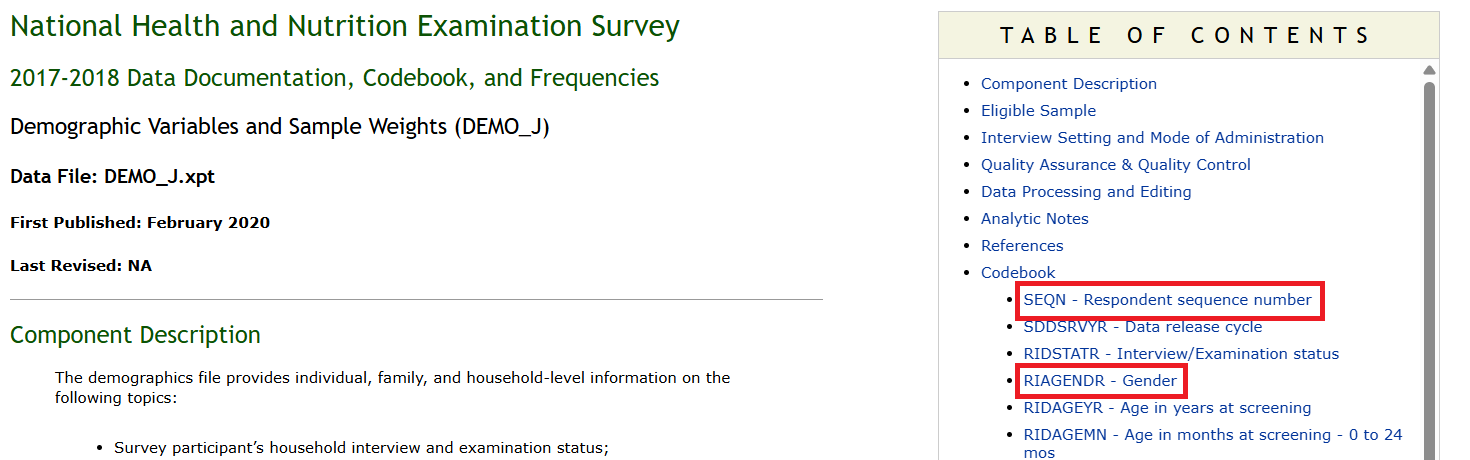
\includegraphics[width=0.9\linewidth,height=\textheight,keepaspectratio]{references/data-sources/../../assets/images/data2/nhanes19.png}
\end{center}

You need to click on the \texttt{SEQN\ -\ Respondent\ sequence\ number}
link or scroll down to find the information about the \texttt{SEQN}
variable.

\begin{center}
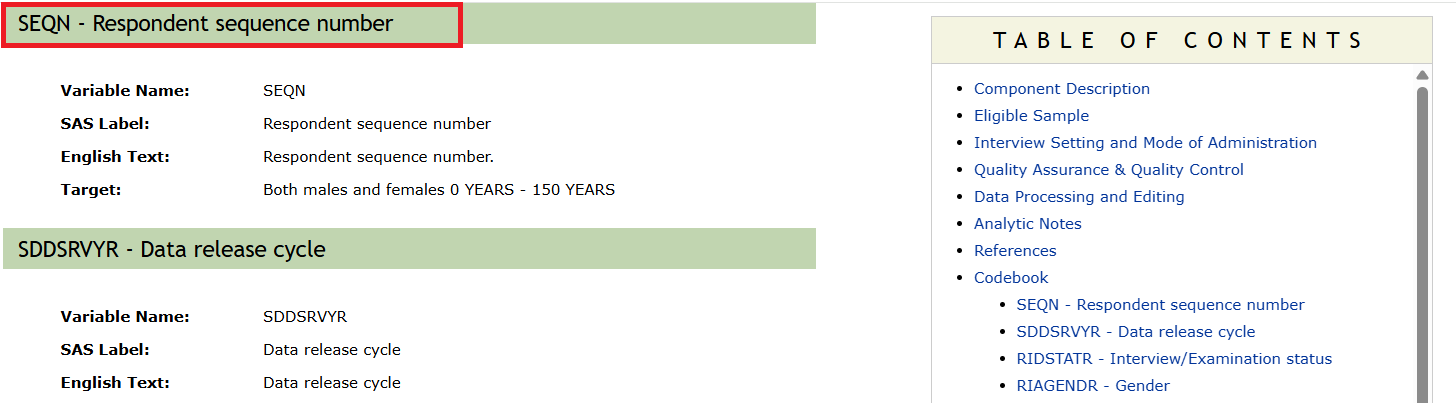
\includegraphics[width=0.9\linewidth,height=\textheight,keepaspectratio]{references/data-sources/../../assets/images/data2/nhanes20.png}
\end{center}

Similarly, you can click on the \texttt{RIAGENDR\ -\ Gender} link or
scroll down to find the information about the \texttt{RIAGENDR}
variable.

\begin{center}
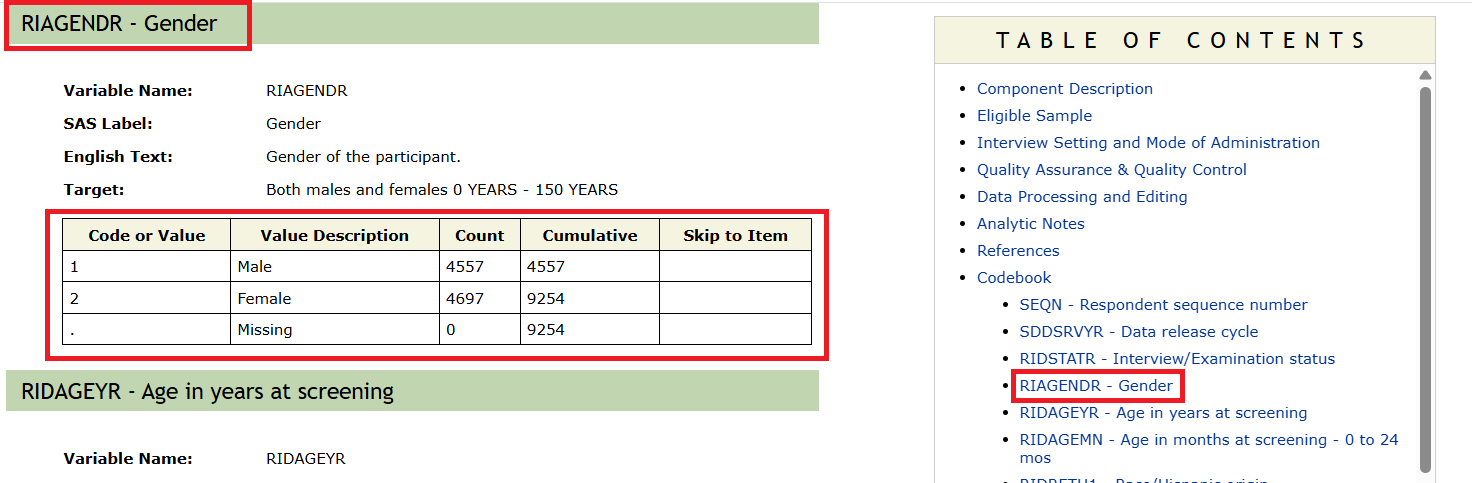
\includegraphics[width=0.9\linewidth,height=\textheight,keepaspectratio]{references/data-sources/../../assets/images/data2/nhanes21.png}
\end{center}

As you can see, the \texttt{RIAGENDR} variable has two values: 1 for
Male and 2 for Female, without any missing values. You can also see the
frequency of each value in the dataset. These numbers/frequencies should
exactly match the frequencies in your dataset. You can use the codebook
to understand other variables in the dataset. Similarly, you can use the
other data files (e.g., Dietary) and their codebook to understand the
variables in those datasets. Unlike the demographic file, which uses
only one dataset and one codebook, the other files use multiple datasets
and codebooks. As an example, if you click on the
\texttt{Questionnaire\ Data} link, you will find multiple datasets and
codebooks for questionnaire data:

\begin{center}
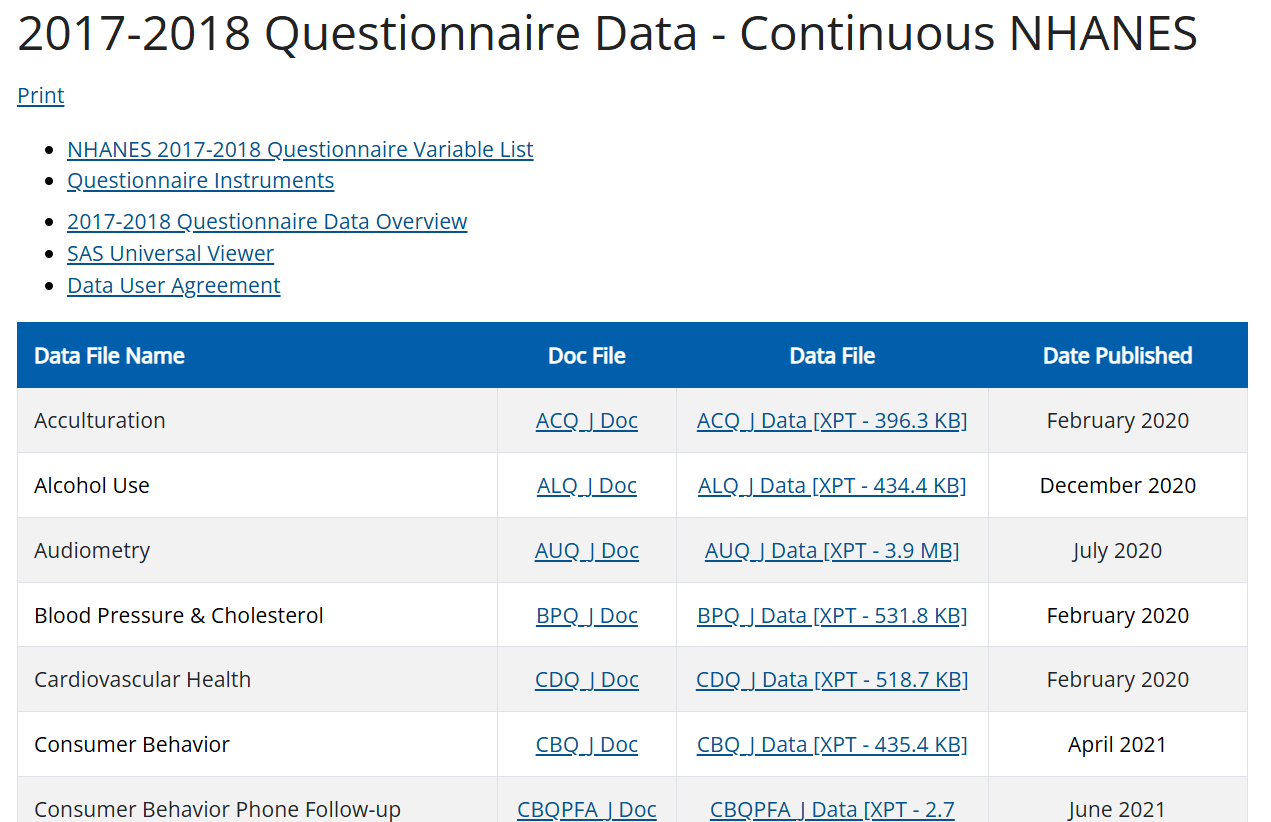
\includegraphics[width=0.9\linewidth,height=\textheight,keepaspectratio]{references/data-sources/../../assets/images/data2/nhanes22.png}
\end{center}

\chapter*{Data Source: BRFSS}\label{data-source-brfss}
\addcontentsline{toc}{chapter}{Data Source: BRFSS}

\markboth{Data Source: BRFSS}{Data Source: BRFSS}

The Behavioral Risk Factor Surveillance System (BRFSS) is a
cross-sectional survey conducted by the US Centers for Disease Control
(CDC). The survey collects information on health-related risk behaviors,
chronic health conditions, and use of preventive services among US
adults. BRFSS completes more than 400,000 adult interviews each year,
making it the largest continuously conducted health survey system in the
world.

\begin{center}
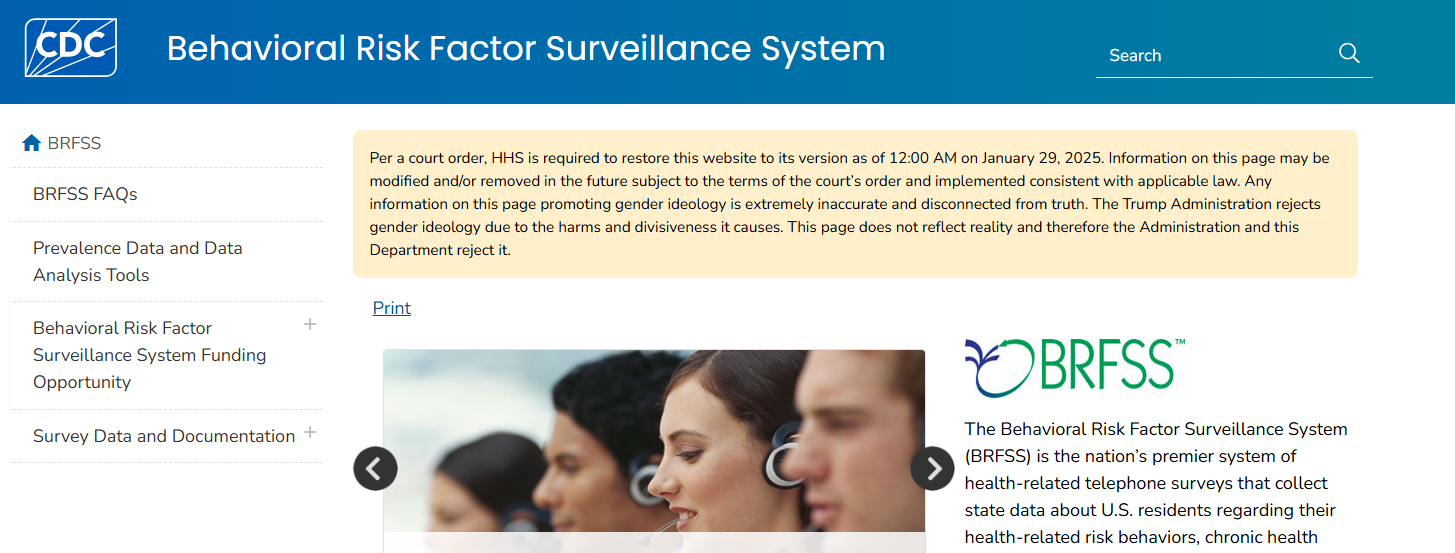
\includegraphics[width=0.9\linewidth,height=\textheight,keepaspectratio]{references/data-sources/../../assets/images/data3/BRFSS1.png}
\end{center}

\marginnote{\begin{footnotesize}

\href{https://www.cdc.gov/brfss/index.html}{CDC website for BRFSS}

\end{footnotesize}}

\subsection*{About BRFSS}\label{about-brfss}
\addcontentsline{toc}{subsection}{About BRFSS}

You can find more information about the BRFSS survey by clicking on
\href{https://www.cdc.gov/brfss/about/brfss_faq.htm}{BRFSS FAQs}:

\begin{center}
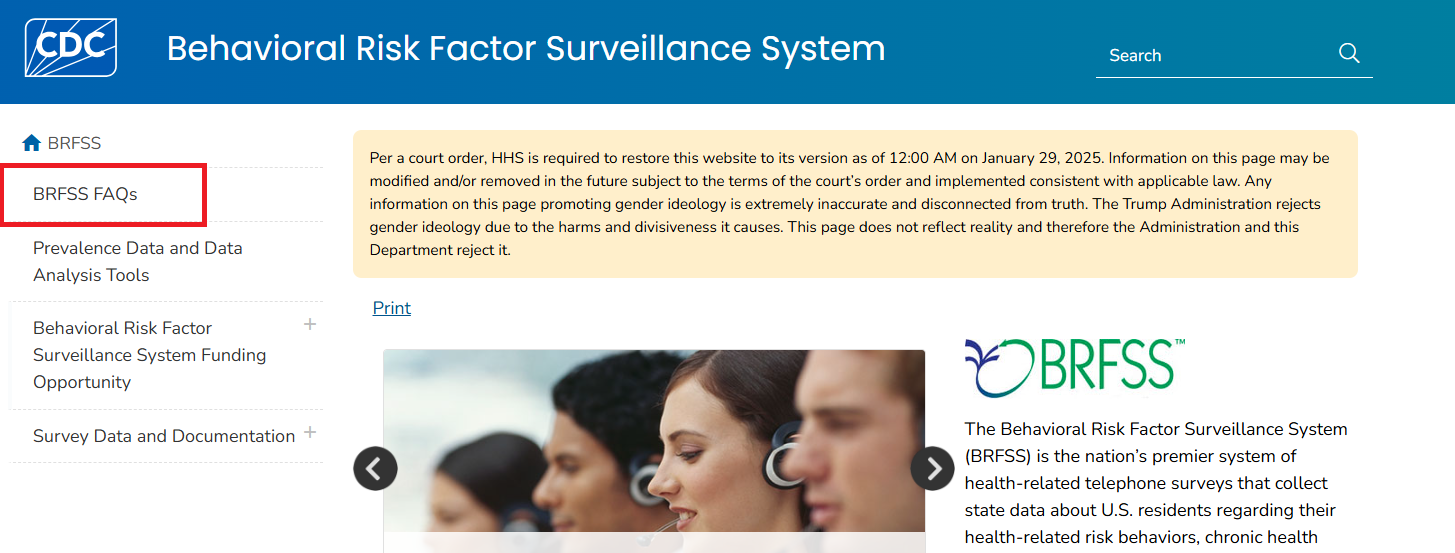
\includegraphics[width=0.9\linewidth,height=\textheight,keepaspectratio]{references/data-sources/../../assets/images/data3/BRFSS2.png}
\end{center}

On the \texttt{BRFSS\ FAQs} page, you will find information about the
BRFSS survey, including what the survey collects, how the survey is
conducted, and how to use the data.

\subsection*{Survey Data \&
Documentation}\label{survey-data-documentation}
\addcontentsline{toc}{subsection}{Survey Data \& Documentation}

If you click on \texttt{Survey\ Data\ \&\ Documentation} link, you will
find information about the BRFSS questionnaires, datasets, and
documentation:

\begin{center}
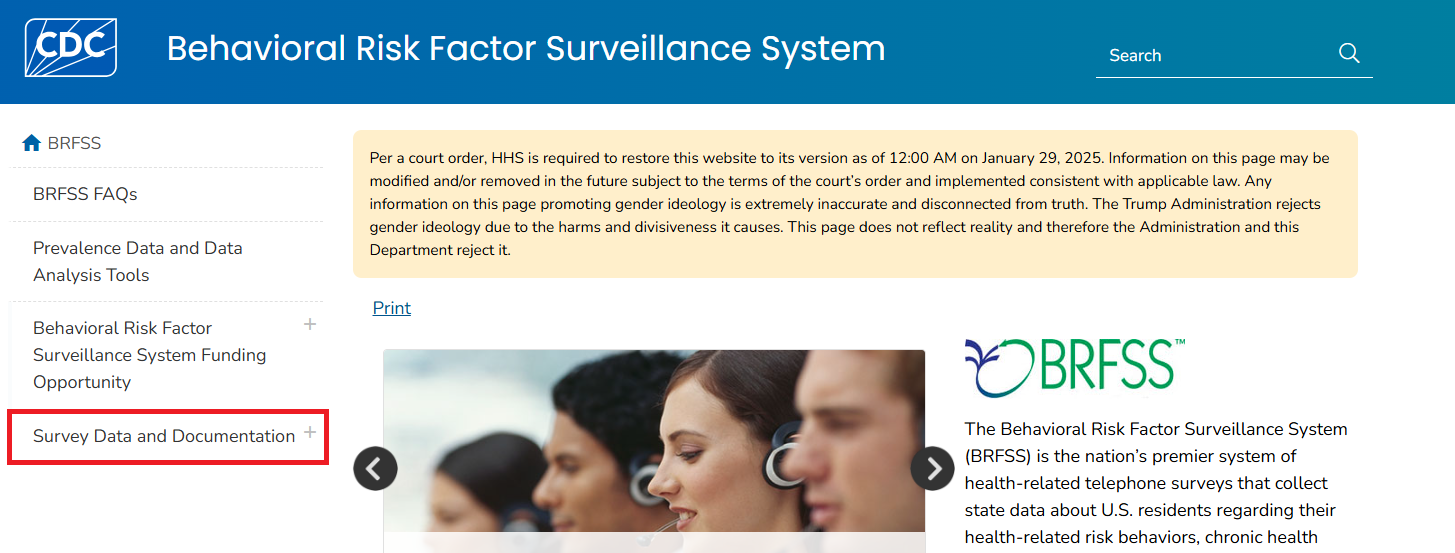
\includegraphics[width=0.9\linewidth,height=\textheight,keepaspectratio]{references/data-sources/../../assets/images/data3/BRFSS3.png}
\end{center}

\marginnote{\begin{footnotesize}

\href{https://www.cdc.gov/brfss/data_documentation/index.htm}{BRFSS
Survey Data \& Documentation}

\end{footnotesize}}

There are four types of data files available for download: 1) annual
data, 2) asthma call-back data, 3) GIS map data, and 4) SMART data. The
annual data files include information on health-related risk behaviors,
chronic health conditions, and use of preventive services among US
adults. The asthma call-back data files include information on
asthma-related health outcomes and healthcare utilization among adults
with asthma. The GIS map data files include information on the
geographic distribution of the data. The SMART (Selected
Metropolitan/Micropolitan Area Risk Trends) data provide prevalence
rates for selected conditions and behaviors for cities and their
surrounding counties.

\begin{center}
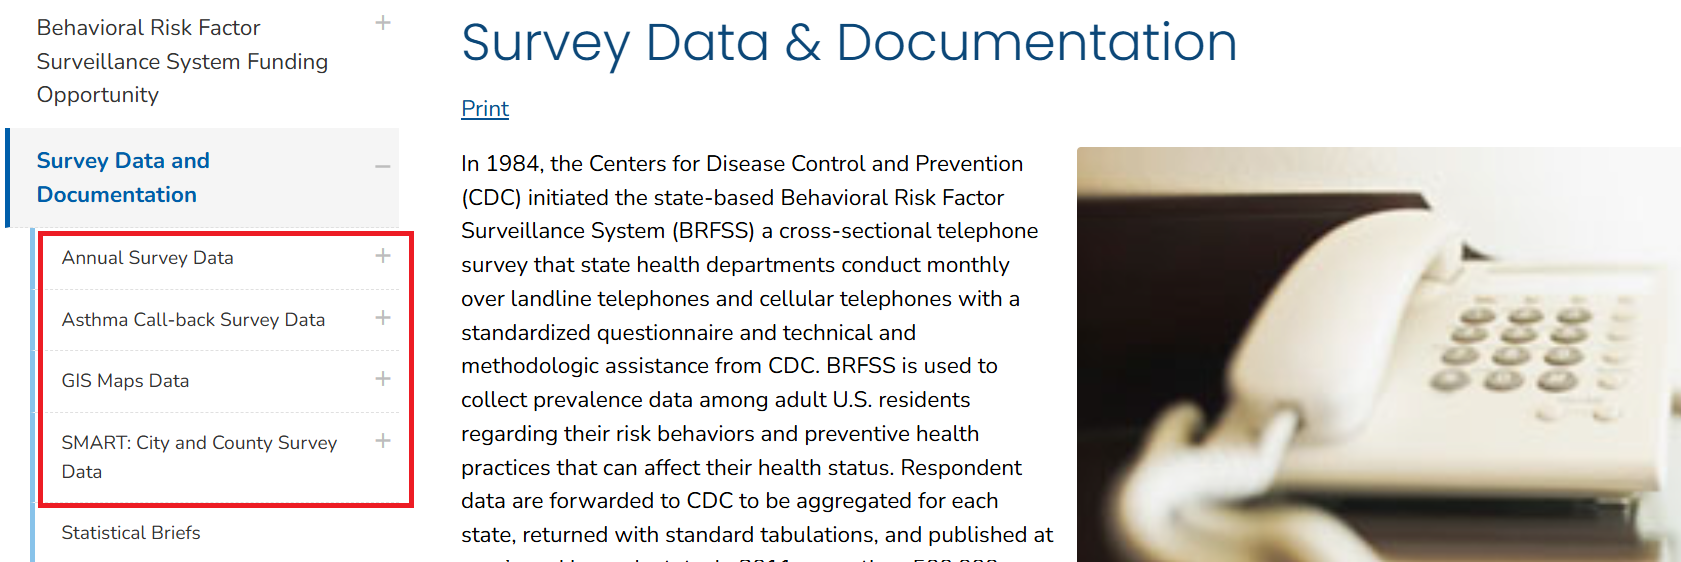
\includegraphics[width=0.9\linewidth,height=\textheight,keepaspectratio]{references/data-sources/../../assets/images/data3/BRFSS4.png}
\end{center}

For the annual data, you can click on the \texttt{Annual\ Survey\ Data}
link to find information about the annual data files, including how to
access the data, how to use the data, and how to analyze the data. There
are two types of annual data files available for download: 1) the raw
data files and 2) the prevalence and trends database.

\begin{center}
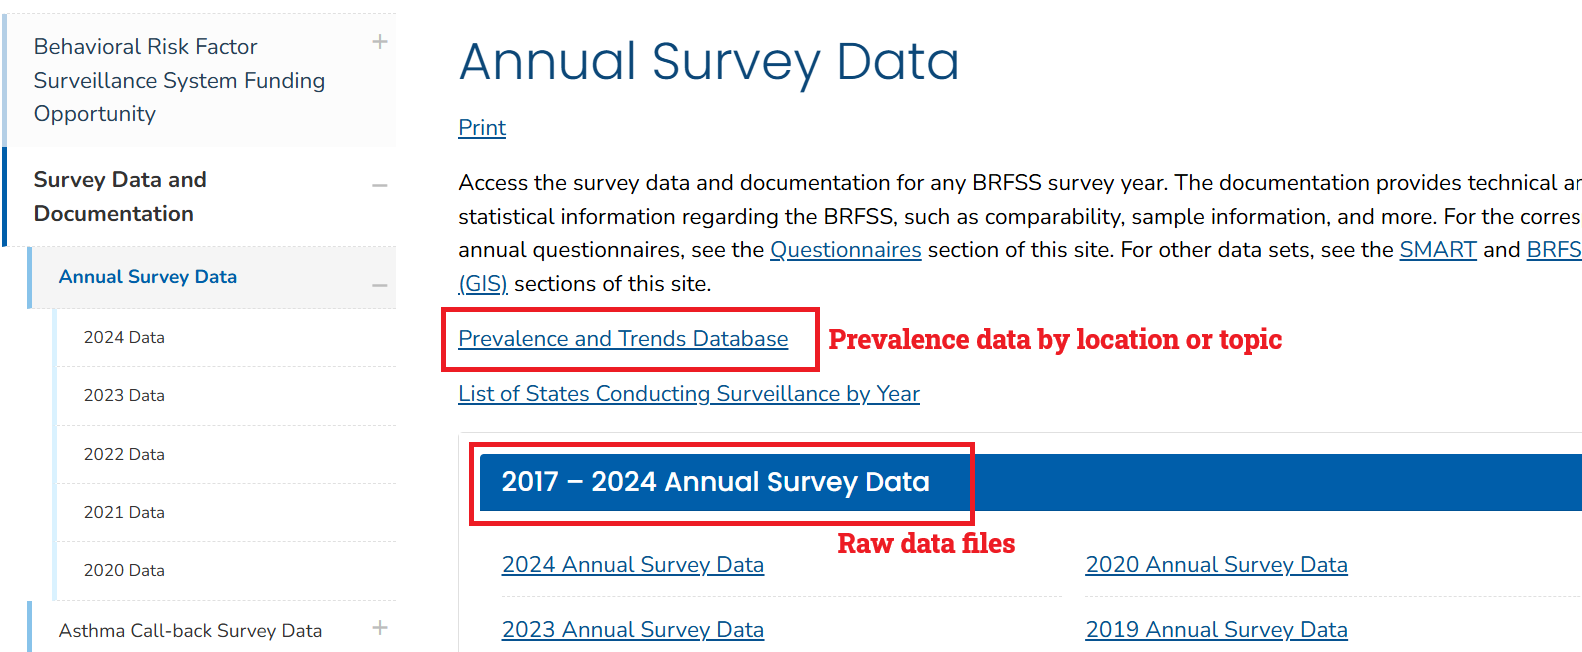
\includegraphics[width=0.9\linewidth,height=\textheight,keepaspectratio]{references/data-sources/../../assets/images/data3/BRFSS5.png}
\end{center}

\subsection*{Annual Survey Data}\label{annual-survey-data}
\addcontentsline{toc}{subsection}{Annual Survey Data}

There are separate links for each year of data, and you can click on
each link to find information about the data for that year. For example,
if you click on the \texttt{2023\ Annual\ Survey\ Data} link, you will
find information about the 2023 annual data files, including how to
access the data, how to use the data, and how to analyze the data.

\marginnote{\begin{footnotesize}

\href{https://www.cdc.gov/brfss/annual_data/annual_data.htm}{Annual
Survey Data}

\end{footnotesize}}

\begin{center}
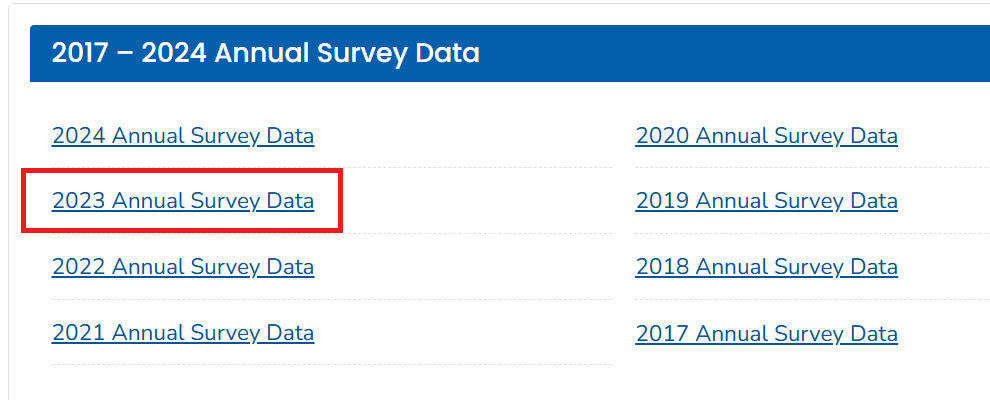
\includegraphics[width=0.9\linewidth,height=\textheight,keepaspectratio]{references/data-sources/../../assets/images/data3/BRFSS6.png}
\end{center}

\begin{center}
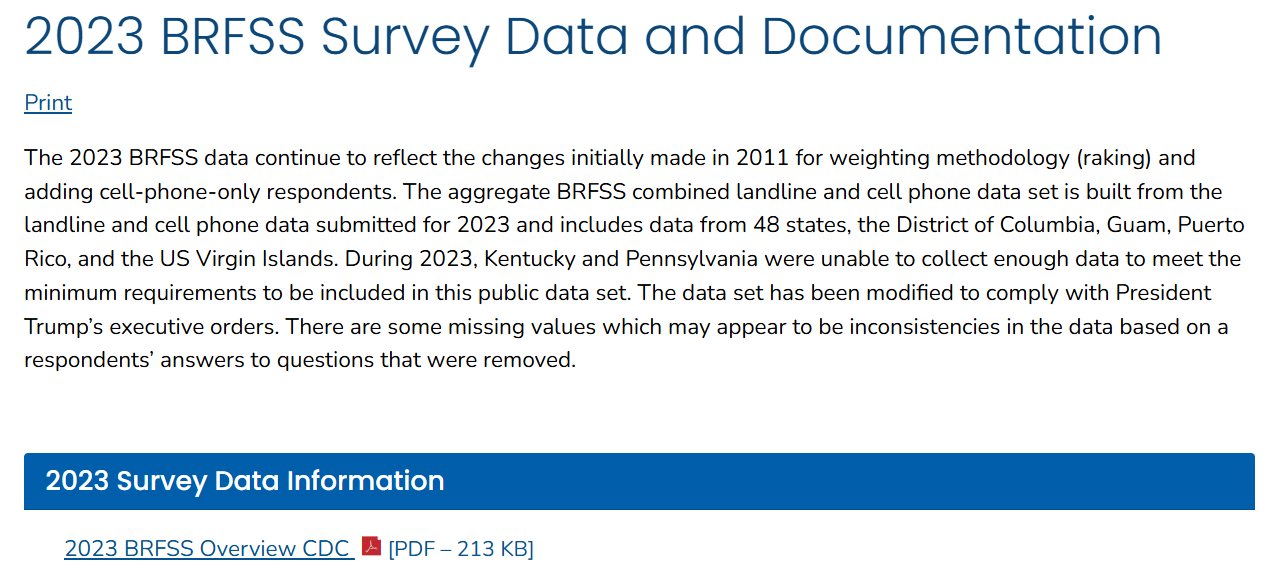
\includegraphics[width=0.9\linewidth,height=\textheight,keepaspectratio]{references/data-sources/../../assets/images/data3/BRFSS7.png}
\end{center}

The \texttt{2023\ BRFSS\ Survey\ Data\ and\ Documentation} page provides
information about three resources: 1) data information such as the
codebook and sampling weights, 2) data files in ASCII and SAS XPT
transport formats, and 3) SAS resources. To download/save the data
files, click the specific format you want. For example, if you click on
the \texttt{2023\ BRFSS\ Data\ (SAS\ Transport\ Format)} link, the
annual survey data for 2023 will be downloaded in a ZIP file that
contains the dataset in a \texttt{.XPT} format.

\begin{center}
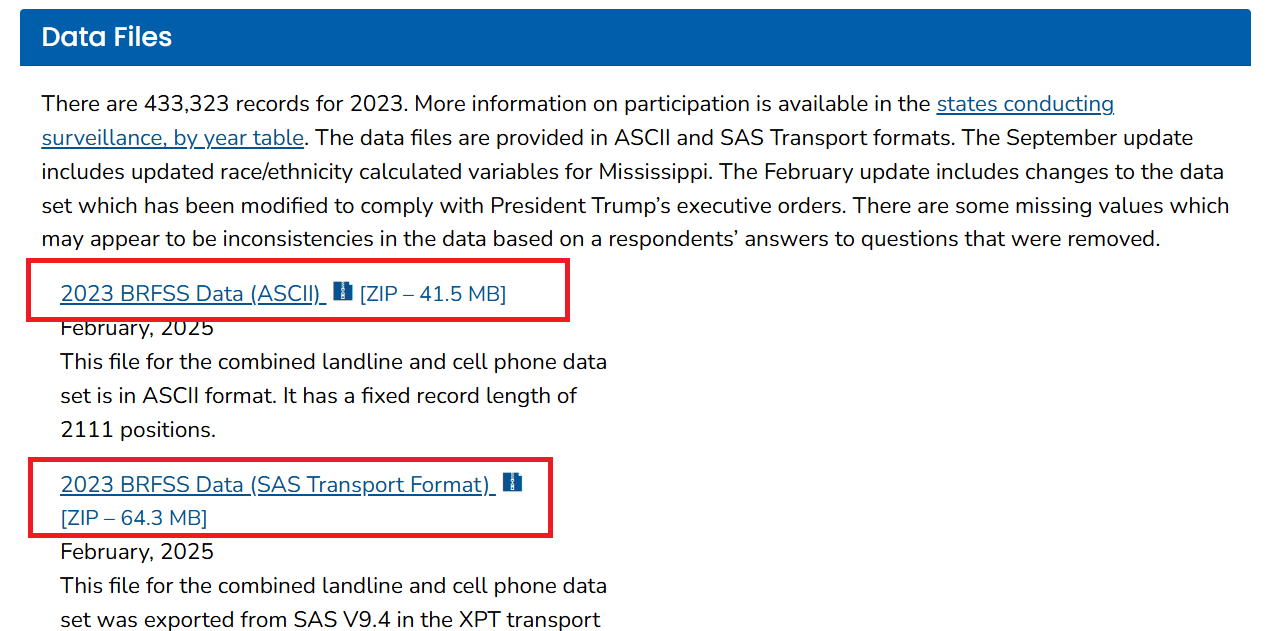
\includegraphics[width=0.9\linewidth,height=\textheight,keepaspectratio]{references/data-sources/../../assets/images/data3/BRFSS8.png}
\end{center}

You need to unzip the file to extract the data file in \texttt{.XPT}
format. However, opening the data file in Excel or Google Sheets is a
bit tricky. The SAS XPT (or ASCII) data file needs to be
converted/formatted appropriately before it can be opened in Excel or
Google Sheets. Many statistical software packages, such as R, SAS, or
STATA, can read the data file in \texttt{.XPT} format. Below is the data
file, where the column names are the variable names, and the rows are
the observations (i.e., survey respondents):

\begin{center}
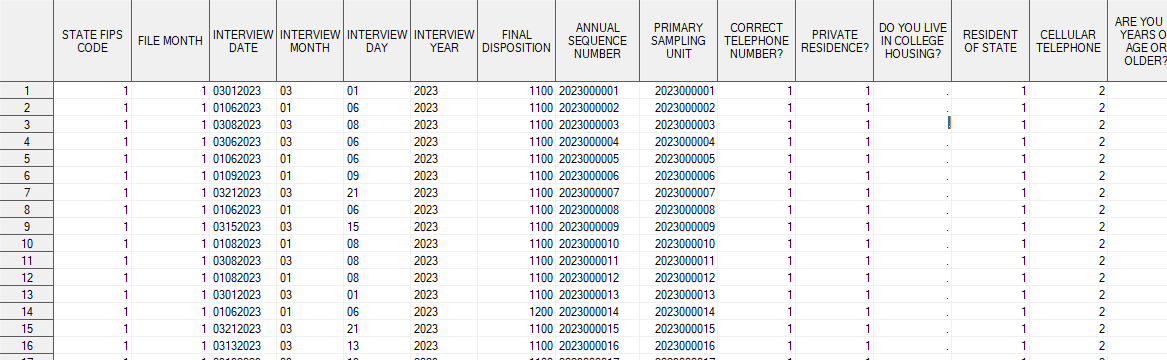
\includegraphics[width=0.9\linewidth,height=\textheight,keepaspectratio]{references/data-sources/../../assets/images/data3/BRFSS9.png}
\end{center}

To understand the variables in the dataset, you can refer to the
codebook:

\begin{center}
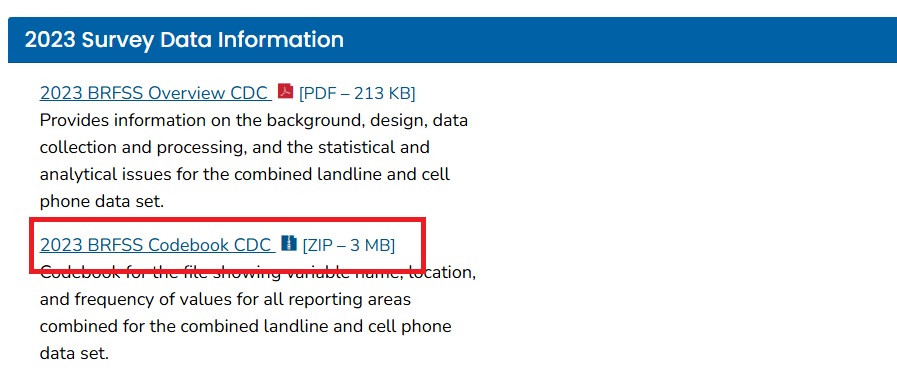
\includegraphics[width=0.9\linewidth,height=\textheight,keepaspectratio]{references/data-sources/../../assets/images/data3/BRFSS10.png}
\end{center}

You need to unzip the file to extract the codebook in HTML format. The
codebook provides information about the variable names, labels, and
values. For example, if you want to understand the variable
\texttt{Drinking\ and\ Driving}, you can find the variable name, label,
and values in the codebook:

\begin{center}
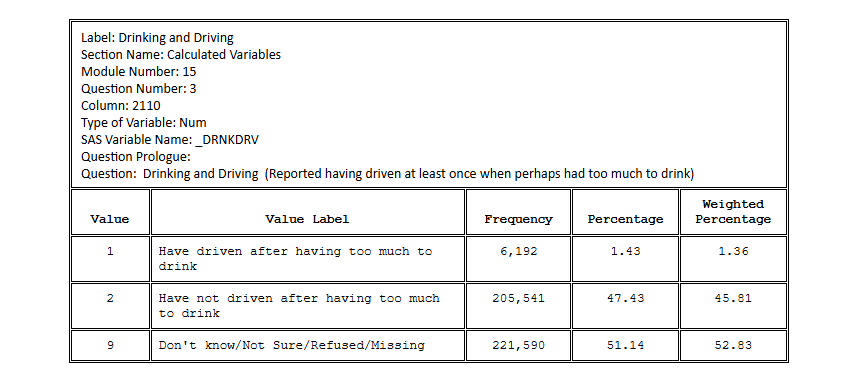
\includegraphics[width=0.9\linewidth,height=\textheight,keepaspectratio]{references/data-sources/../../assets/images/data3/BRFSS11.png}
\end{center}

You can similarly download the asthma call-back, GIS map, and SMART
datasets. To understand the variables in those datasets, you can refer
to the codebook for each dataset.

\marginnote{\begin{footnotesize}

\href{https://www.cdc.gov/brfss/acbs/index.htm}{Asthma Call-back Data}

\href{https://www.cdc.gov/brfss/gis/gis_maps.htm}{GIS Data}

\href{https://www.cdc.gov/brfss/smart/Smart_data.htm}{SMART Data}

\end{footnotesize}}

\subsection*{Prevalence and Trends
Database}\label{prevalence-and-trends-database}
\addcontentsline{toc}{subsection}{Prevalence and Trends Database}

The BRFSS prevalence and trends tool allows users to view and download
prevalence estimates through charts, graphs, and maps. You can explore
the estimates by selecting the topic or location. For example, if you
select \texttt{by\ topic}, e.g., for alcohol consumption for Alabama for
the year 2024, you need to select the options from the dropdown menu and
click on the \texttt{View\ Results} button to see the results:

\marginnote{\begin{footnotesize}

\href{https://www.cdc.gov/brfss/brfssprevalence/index.html}{Prevalence
and Trends Database}

\end{footnotesize}}

\begin{center}
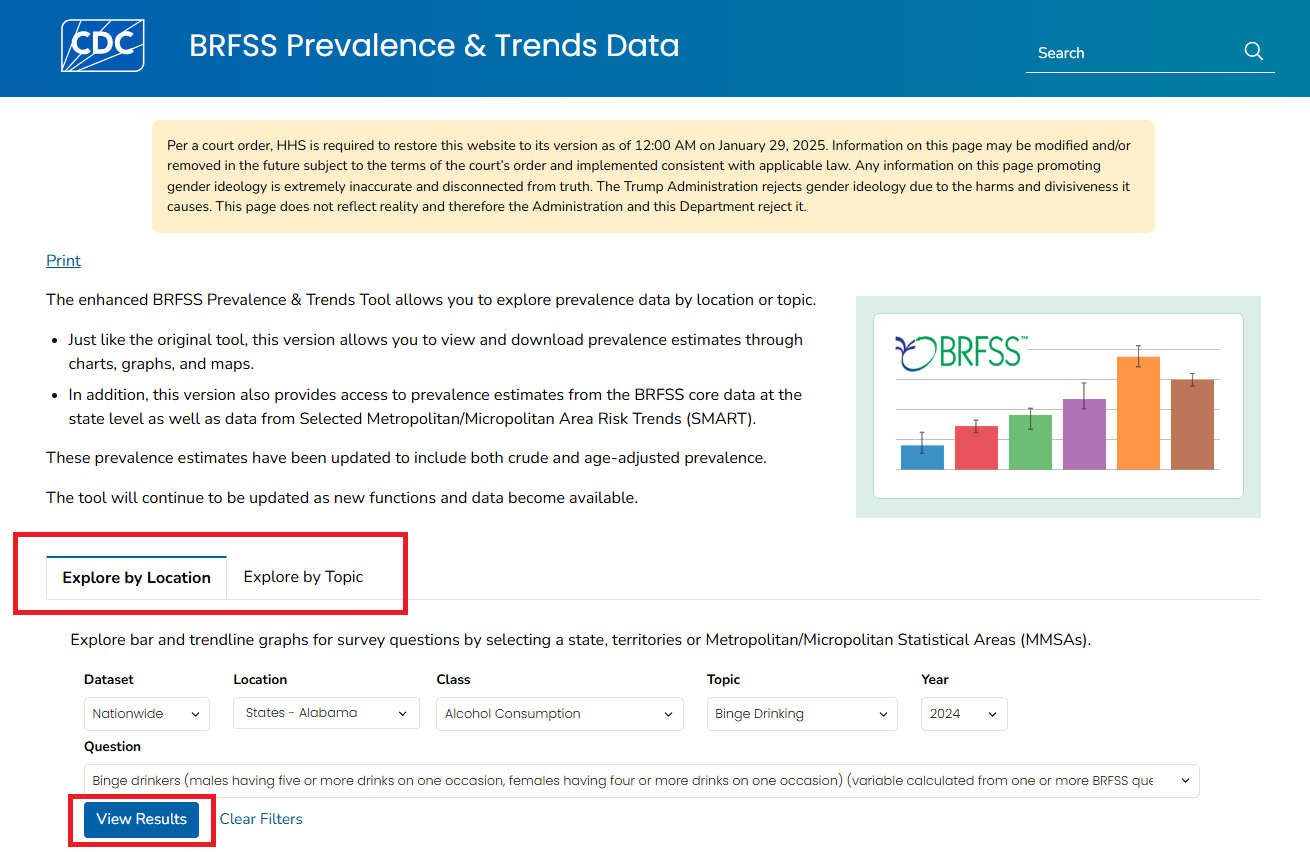
\includegraphics[width=0.9\linewidth,height=\textheight,keepaspectratio]{references/data-sources/../../assets/images/data3/BRFSS12.png}
\end{center}

The results will show the (i) prevalence estimates for alcohol
consumption in Alabama for the year 2024, and (ii) the trend of alcohol
consumption in Alabama over time.

\begin{center}
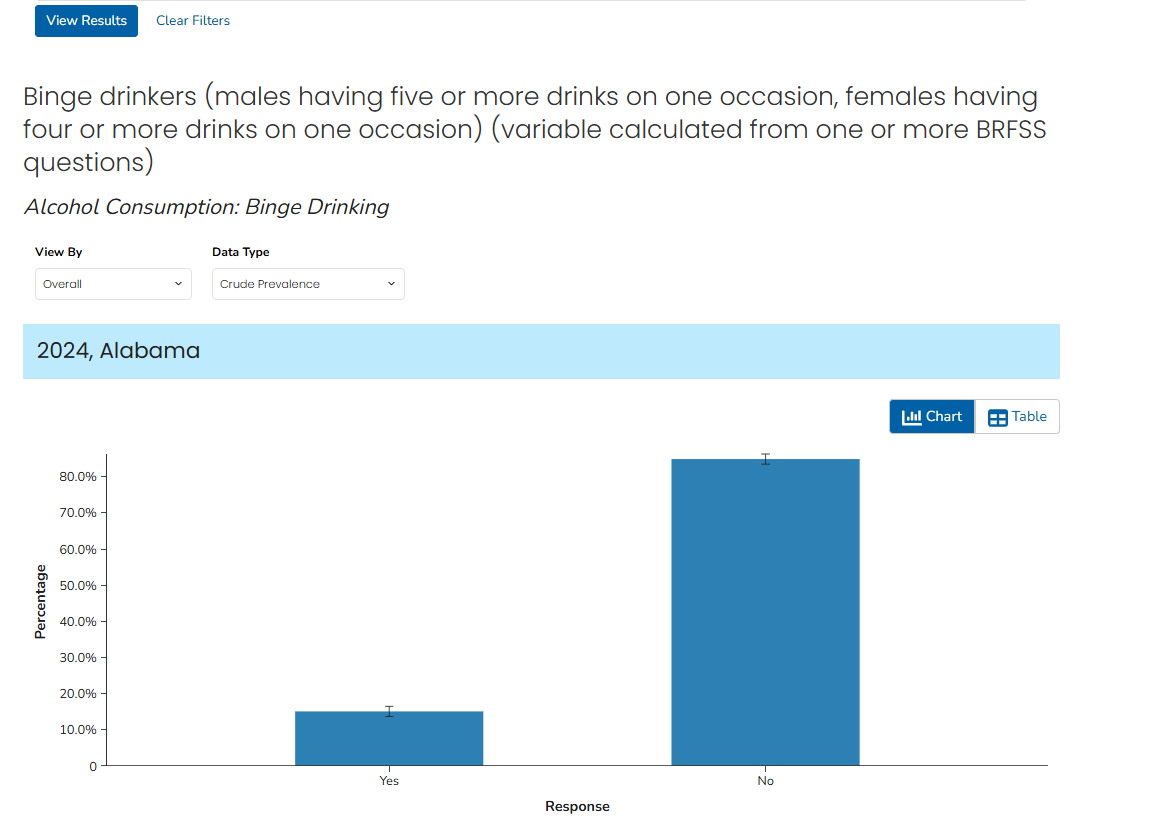
\includegraphics[width=0.9\linewidth,height=\textheight,keepaspectratio]{references/data-sources/../../assets/images/data3/BRFSS13.png}
\end{center}

\begin{center}
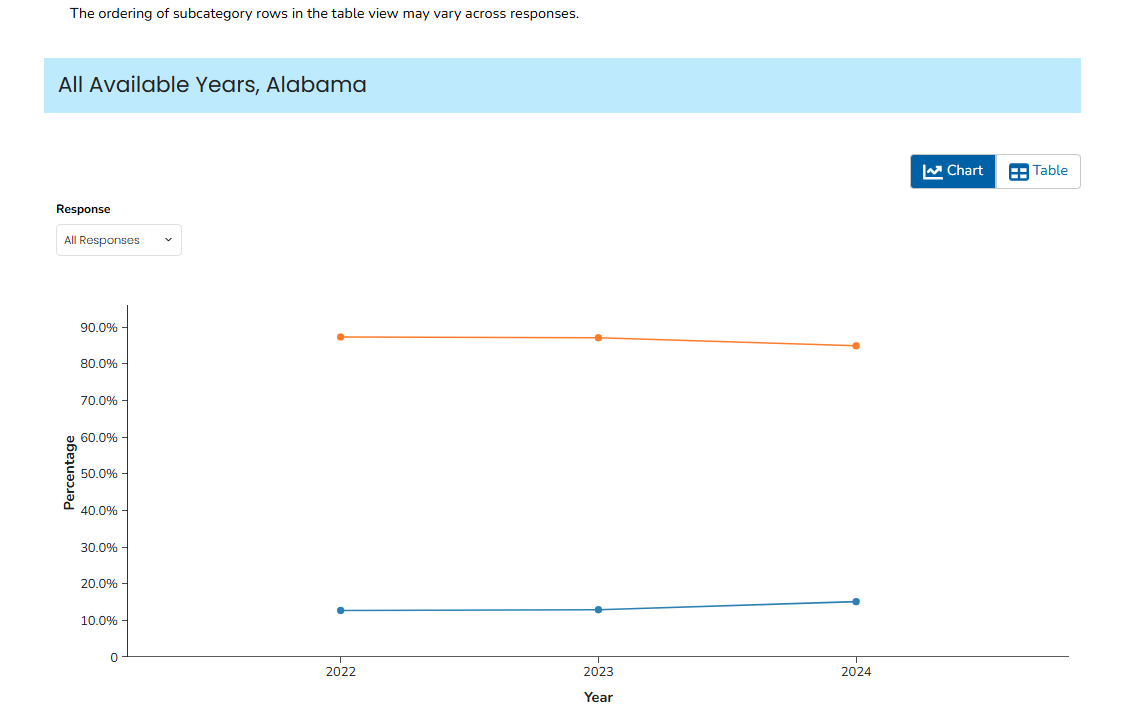
\includegraphics[width=0.9\linewidth,height=\textheight,keepaspectratio]{references/data-sources/../../assets/images/data3/BRFSS14.png}
\end{center}

\chapter*{Data Source: CCS}\label{data-source-ccs}
\addcontentsline{toc}{chapter}{Data Source: CCS}

\markboth{Data Source: CCS}{Data Source: CCS}

The Canadian Cannabis Survey (CCS) is an annual survey conducted by
Health Canada to gather information on cannabis use among people aged 16
years and older living in all Canadian provinces and territories. The
survey collects data on various aspects of cannabis consumption,
including their knowledge, attitudes and behaviours towards cannabis
use.

\begin{center}

\includegraphics[width=0.9\linewidth,height=\textheight,keepaspectratio]{references/data-sources/../../assets/images/data4/ccs1.png}
\end{center}

\marginnote{\begin{footnotesize}

\href{https://open.canada.ca/data/dataset/2abe0796-c3e6-443b-a5c5-74e770e9fbe0}{Health
Canada website for CCS}

\end{footnotesize}}

More than 11,000 respondents participated in the 2024 survey. The study
provides valuable insights into cannabis use patterns, the cannabis
market, and issues of public safety. The survey results are published on
Health Canada's website:

\begin{center}
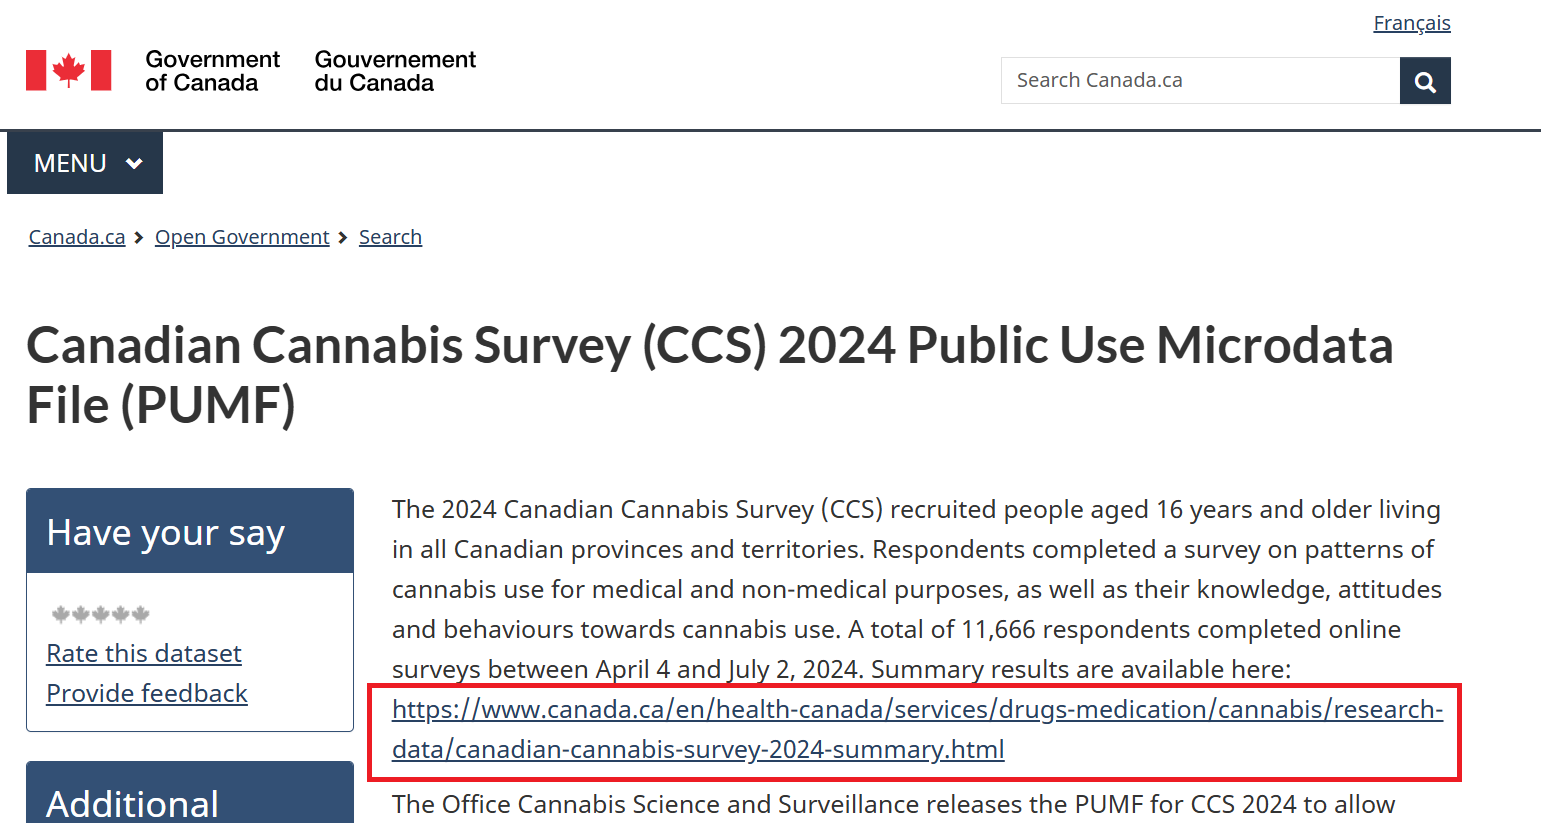
\includegraphics[width=0.9\linewidth,height=\textheight,keepaspectratio]{references/data-sources/../../assets/images/data4/ccs2.png}
\end{center}

\begin{center}
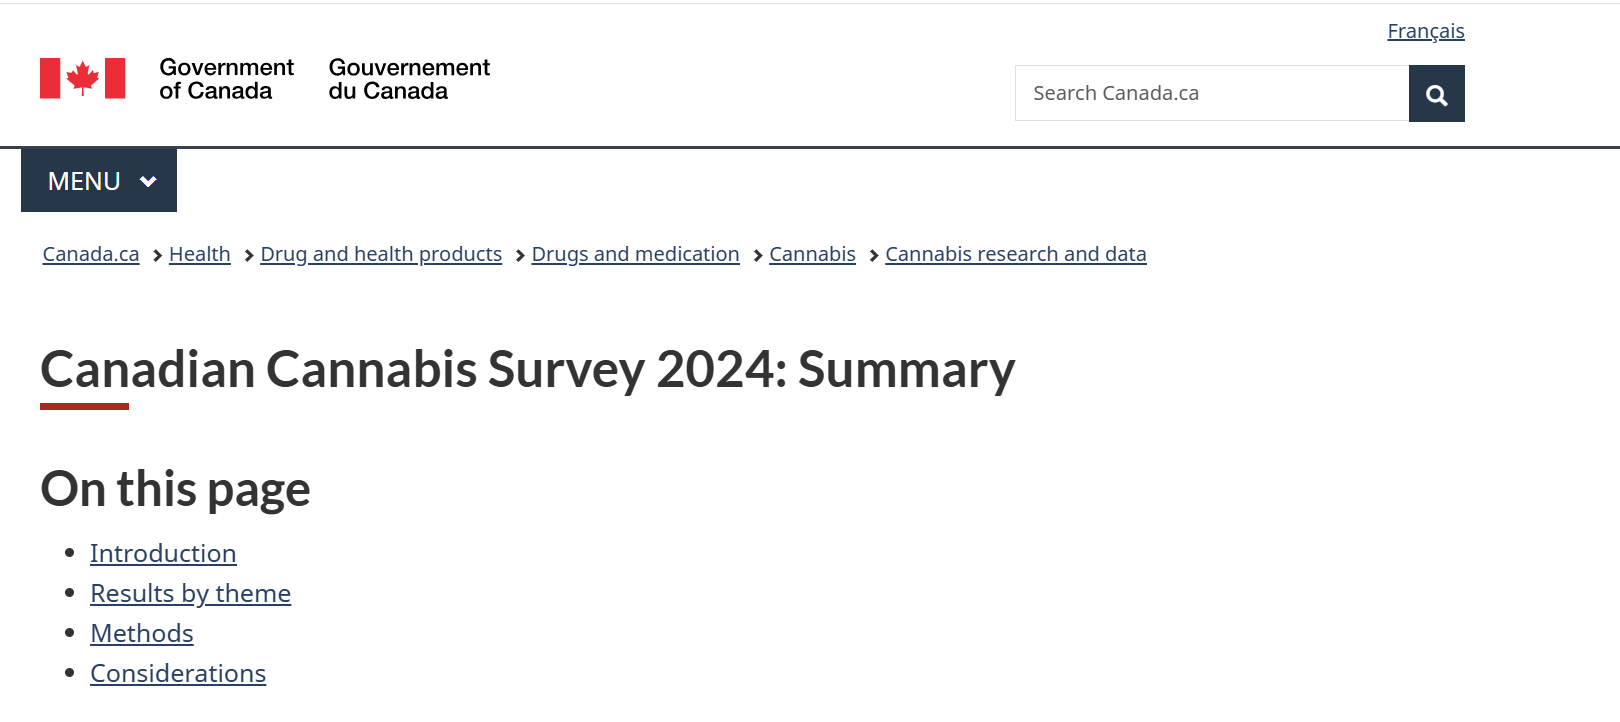
\includegraphics[width=0.9\linewidth,height=\textheight,keepaspectratio]{references/data-sources/../../assets/images/data4/ccs3.png}
\end{center}

\subsection*{Open Licence}\label{open-licence}
\addcontentsline{toc}{subsection}{Open Licence}

The data from the Canadian Cannabis Survey is available under the Open
Government Licence - Canada (OGL-Canada). This licence allows users to
freely use, modify, and distribute the data, provided that they
attribute the source of the data and do not use it for commercial
purposes. The OGL-Canada promotes transparency and encourages the use of
government data for research, analysis, and public benefit. You can
follow the \texttt{Open\ Government\ Licence\ -\ Canada} link for more
information on the terms and conditions of the licence.

\marginnote{\begin{footnotesize}

\href{https://open.canada.ca/en/open-government-licence-canada}{Open
Licence}

\end{footnotesize}}

\begin{center}
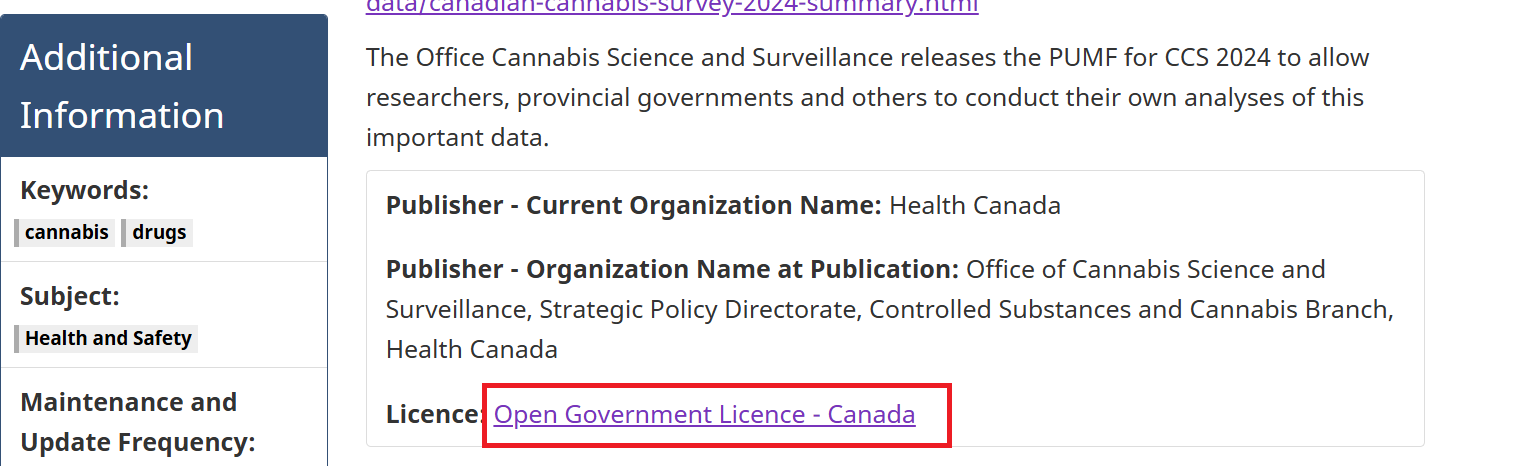
\includegraphics[width=0.9\linewidth,height=\textheight,keepaspectratio]{references/data-sources/../../assets/images/data4/ccs4.png}
\end{center}

\begin{center}

\includegraphics[width=0.9\linewidth,height=\textheight,keepaspectratio]{references/data-sources/../../assets/images/data4/ccs5.png}
\end{center}

\subsection*{Data and Resources}\label{data-and-resources}
\addcontentsline{toc}{subsection}{Data and Resources}

The \texttt{Data\ and\ Resources} tab on the Health Canada website
provides access to the public use data, user guides, and the data
dictionary.

\begin{center}
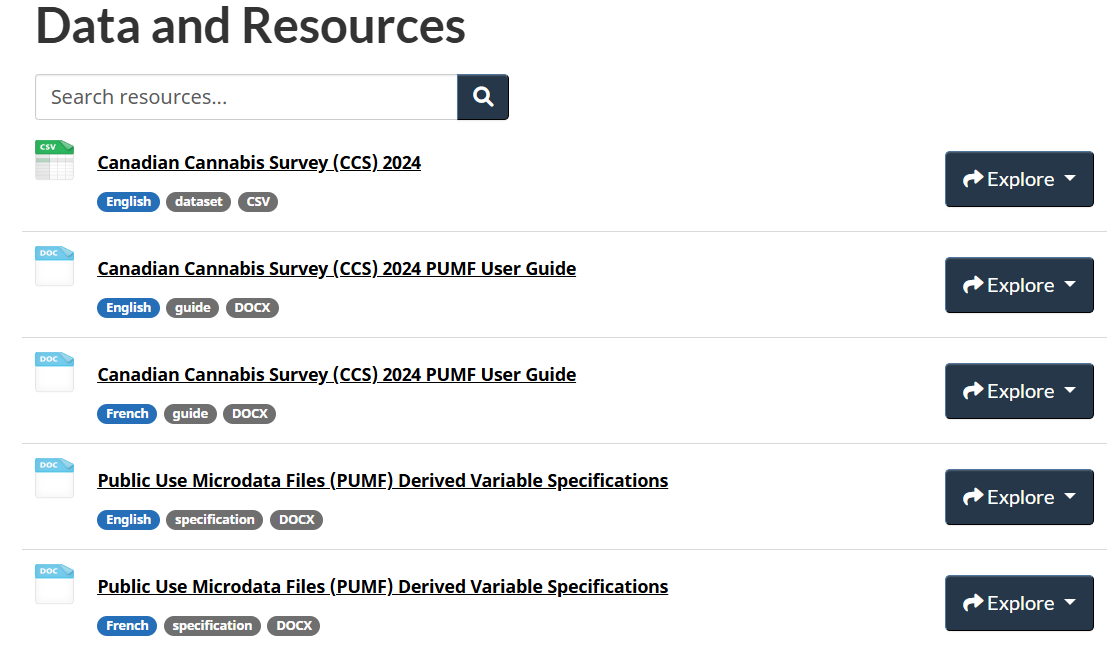
\includegraphics[width=0.9\linewidth,height=\textheight,keepaspectratio]{references/data-sources/../../assets/images/data4/ccs6.png}
\end{center}

The CCS 2024 data is available to download in various formats, including
CSV, TSV, JSON, and XML. The data can be accessed through the Health
Canada website, where you can choose the format that best suits your
needs. You need to open the data link (say, in a new tab in your
browser) and select the desired format to download the data.

\begin{center}
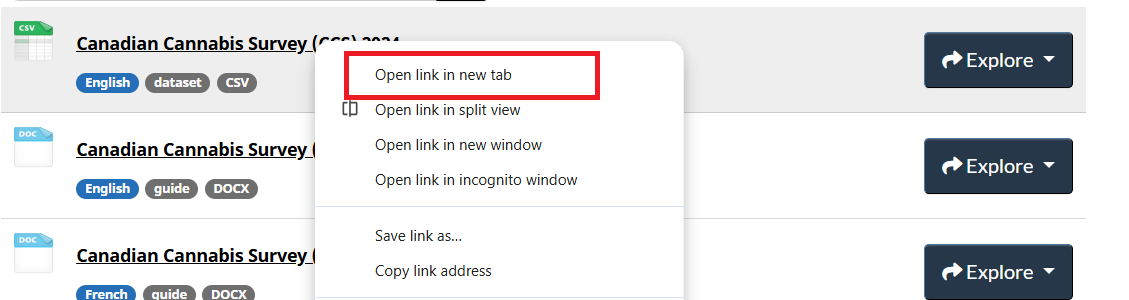
\includegraphics[width=0.9\linewidth,height=\textheight,keepaspectratio]{references/data-sources/../../assets/images/data4/ccs7.png}
\end{center}

Under the \texttt{Download} tab, you can find the data in different
formats. For example, you can download the data in CSV format by
clicking on the \texttt{CSV} link:

\begin{center}
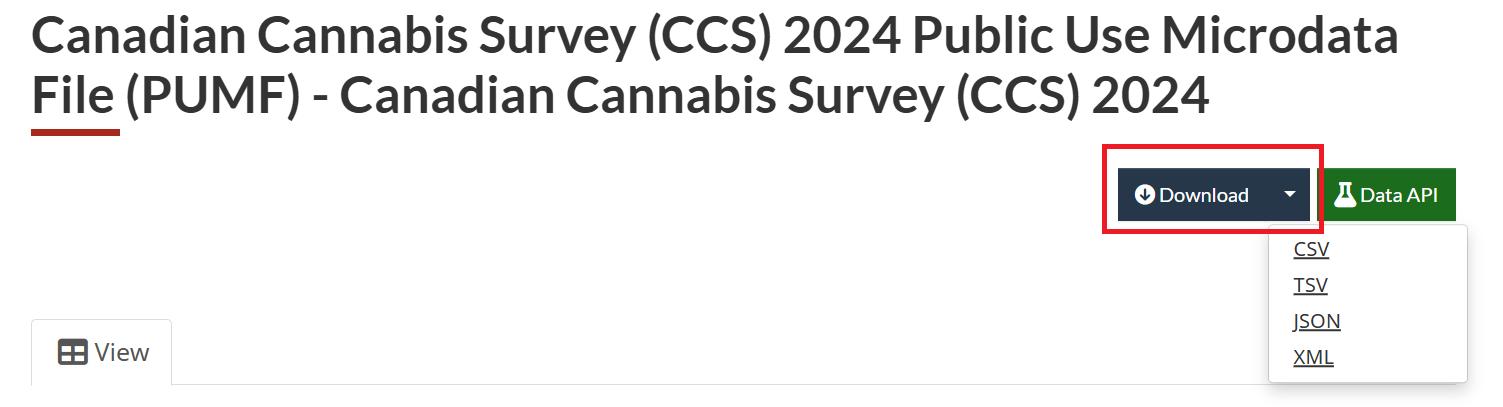
\includegraphics[width=0.9\linewidth,height=\textheight,keepaspectratio]{references/data-sources/../../assets/images/data4/ccs8.png}
\end{center}

After downloading, you can open the data in Excel, Google Sheets, or any
statistical software. The data is structured in a tabular format, with
each row representing an individual respondent and each column
representing different variables:

\begin{center}
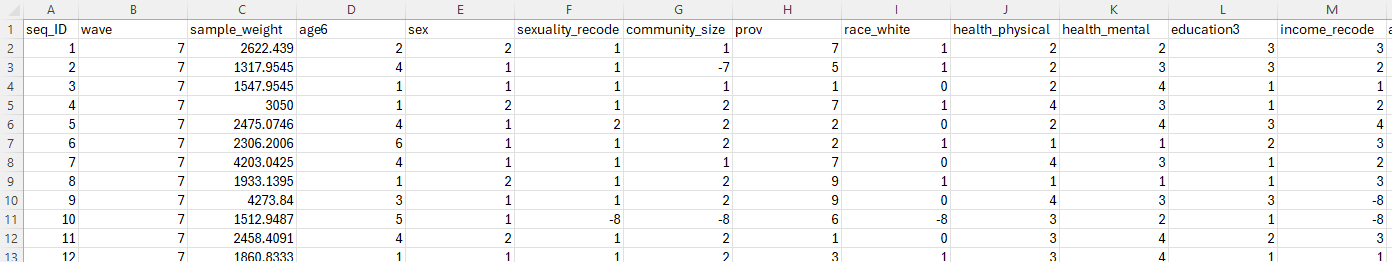
\includegraphics[width=0.9\linewidth,height=\textheight,keepaspectratio]{references/data-sources/../../assets/images/data4/ccs9.png}
\end{center}

The \texttt{Canadian\ Cannabis\ Survey\ (CCS)\ 2024\ PUMF\ User\ Guide}
gives detailed information on the survey methodology, data collection
process, and how to use the public use microdata file (PUMF). You can
also find the variable names and their descriptions in this file.

\marginnote{\begin{footnotesize}

\href{https://open.canada.ca/data/dataset/2abe0796-c3e6-443b-a5c5-74e770e9fbe0/resource/0629eaec-7ba7-492d-9322-d20dc80e55d8}{2024
Public Use Microdata File}

\end{footnotesize}}

\begin{center}
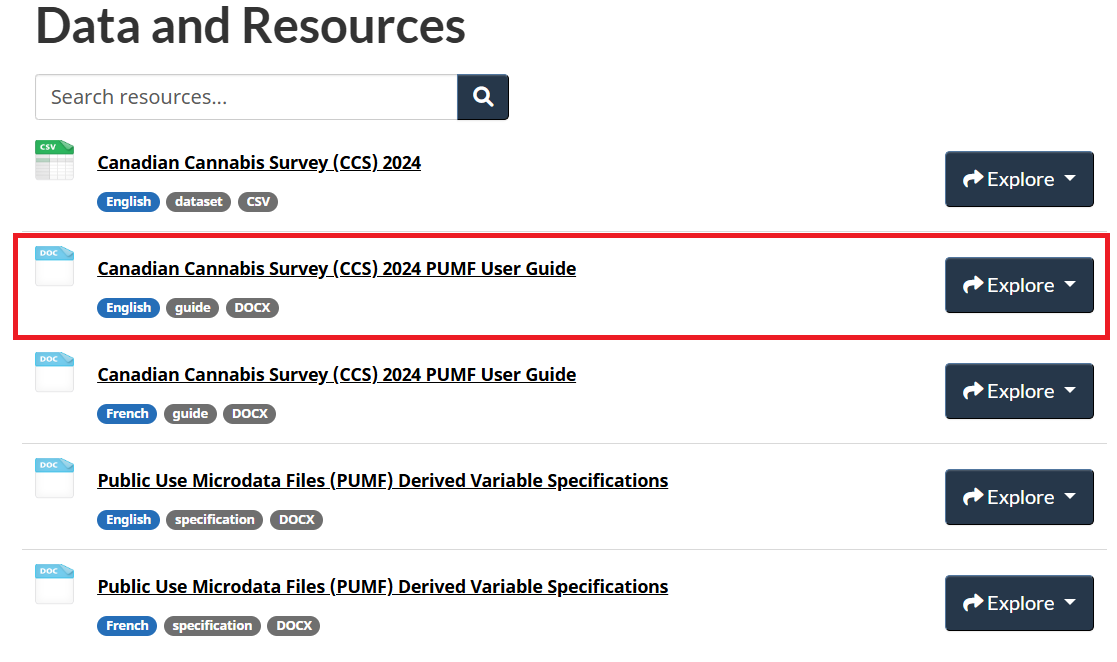
\includegraphics[width=0.9\linewidth,height=\textheight,keepaspectratio]{references/data-sources/../../assets/images/data4/ccs10.png}
\end{center}

Let's find a variable (\texttt{access\_ease\_legal}) in the Excel file
and check its description in the data dictionary. You can use the
\texttt{Find} function in Excel (\texttt{Ctrl\ +\ F}) to search for the
variable name:

\begin{center}
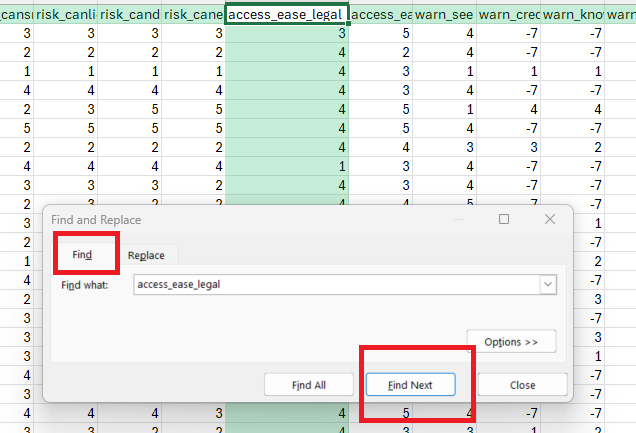
\includegraphics[width=0.9\linewidth,height=\textheight,keepaspectratio]{references/data-sources/../../assets/images/data4/ccs11.png}
\end{center}

Then you can see the description of the variable in the
\texttt{Canadian\ Cannabis\ Survey\ (CCS)\ 2024\ PUMF\ User\ Guide},
which provides information on what the variable represents and how it
was coded:

\begin{center}
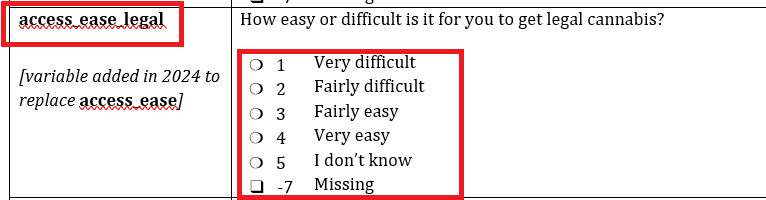
\includegraphics[width=0.9\linewidth,height=\textheight,keepaspectratio]{references/data-sources/../../assets/images/data4/ccs12.png}
\end{center}

In this dataset, \texttt{-7} generally represents missing. Always check
the data dictionary for the specific coding of missing values, ``don't
know,'' or ``refused'' responses, as they can vary between datasets.

\chapter*{Data Source: CADS}\label{data-source-cads}
\addcontentsline{toc}{chapter}{Data Source: CADS}

\markboth{Data Source: CADS}{Data Source: CADS}

The Canadian Alcohol and Drugs Survey (CADS) is a national survey
conducted by Statistics Canada that collects data on the use of
substances, such as alcohol, cannabis and other drugs. The study was
conducted by Statistics Canada in 2019 with the cooperation and support
of Health Canada. The target population for the survey was all persons
aged 15 years and over living in Canada, excluding residents of the
Yukon, Northwest Territories, and Nunavut, full-time residents of
institutions, and residents of Native reserves.

\begin{center}
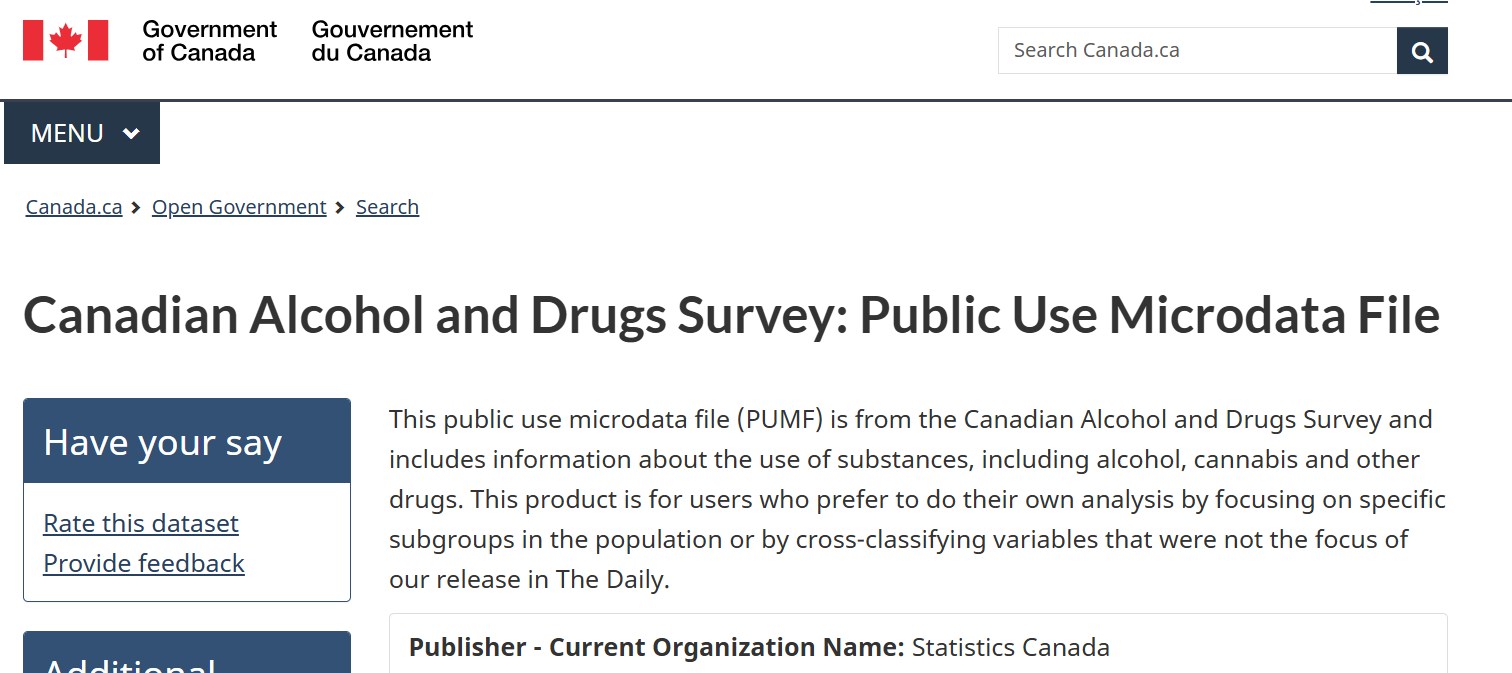
\includegraphics[width=0.9\linewidth,height=\textheight,keepaspectratio]{references/data-sources/../../assets/images/data5/cads1.png}
\end{center}

\marginnote{\begin{footnotesize}

\href{https://ouvert.canada.ca/data/dataset/5c1d47e4-d2be-49d9-9a23-c38f79490fad}{Health
Canada website for CADS}

\end{footnotesize}}

\marginnote{\begin{footnotesize}

\href{https://www.canada.ca/en/health-canada/services/canadian-alcohol-drugs-survey/2019-summary.html}{CADS
2019 summary of results}

\end{footnotesize}}

\subsection*{Open Licence}\label{open-licence-1}
\addcontentsline{toc}{subsection}{Open Licence}

Similar to the
\href{https://open.canada.ca/data/dataset/2abe0796-c3e6-443b-a5c5-74e770e9fbe0}{Canadian
Cannabis Survey}, the CADS is also licensed under the
\href{https://open.canada.ca/en/open-government-licence-canada}{Open
Government Licence - Canada}. This means that the data can be freely
used, modified, and shared by anyone for any purpose, as long as they
provide proper attribution to the source of the data.

\begin{center}
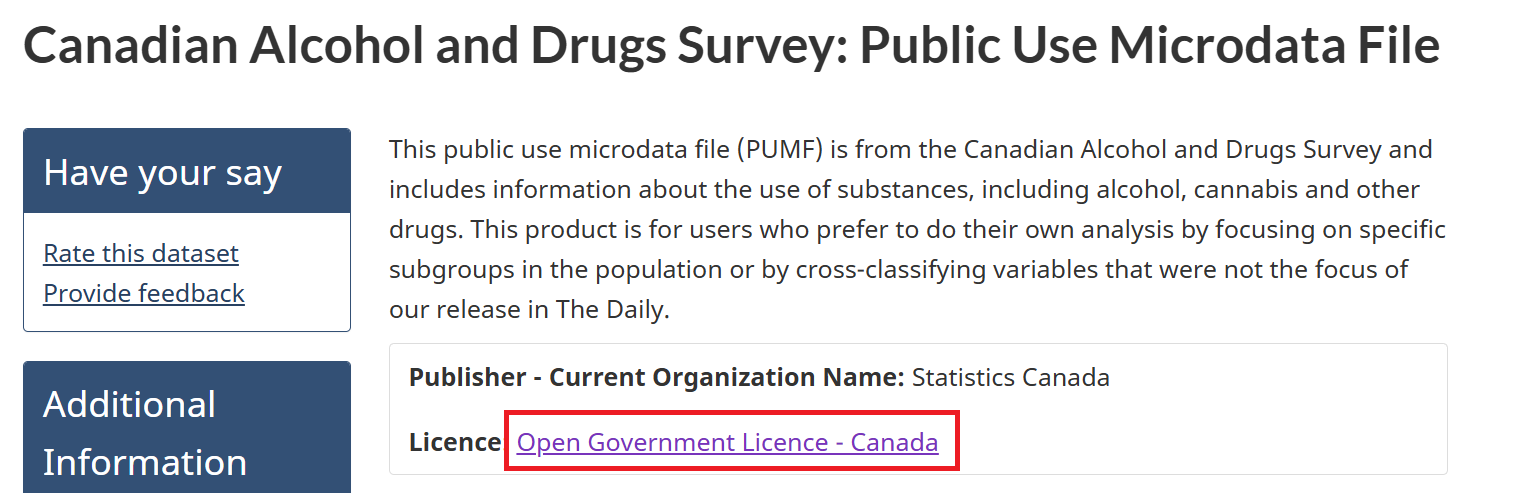
\includegraphics[width=0.9\linewidth,height=\textheight,keepaspectratio]{references/data-sources/../../assets/images/data5/cads2.png}
\end{center}

\begin{center}

\includegraphics[width=0.9\linewidth,height=\textheight,keepaspectratio]{references/data-sources/../../assets/images/data5/cads3.png}
\end{center}

\subsection*{Data and Resources}\label{data-and-resources-1}
\addcontentsline{toc}{subsection}{Data and Resources}

The \texttt{Data\ and\ Resources} tab provides access to the public use
data, user guides, and the data dictionary.

\begin{center}
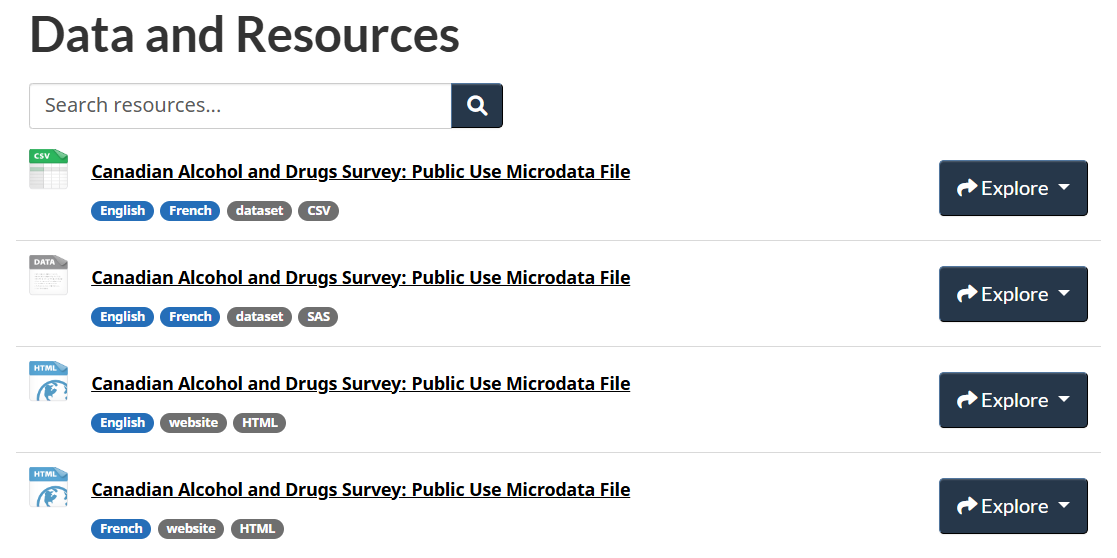
\includegraphics[width=0.9\linewidth,height=\textheight,keepaspectratio]{references/data-sources/../../assets/images/data5/cads4.png}
\end{center}

The public use data file is available in a ZIP format. You need to open
the
\texttt{Canadian\ Alcohol\ and\ Drugs\ Survey:\ Public\ Use\ Microdata\ File}
link, and click on \texttt{Go\ to\ resource}to download the ZIP file.

\begin{center}
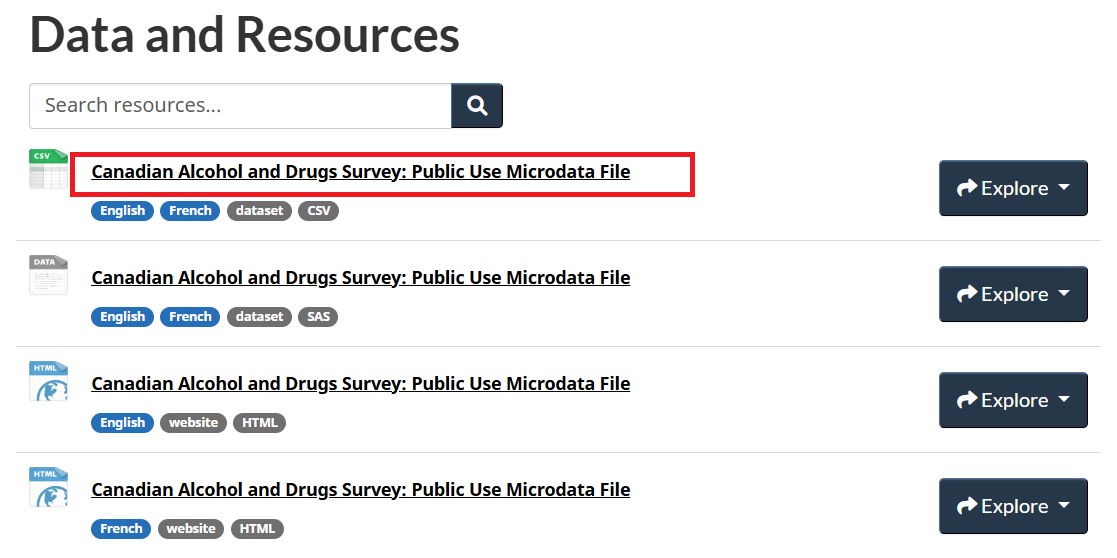
\includegraphics[width=0.9\linewidth,height=\textheight,keepaspectratio]{references/data-sources/../../assets/images/data5/cads5.png}
\end{center}

\begin{center}

\includegraphics[width=0.9\linewidth,height=\textheight,keepaspectratio]{references/data-sources/../../assets/images/data5/cads6.png}
\end{center}

The ZIP file contains the following files: an instruction on how to cite
CADS 2019, data documentation, and the dataset in CSV format.

\begin{center}
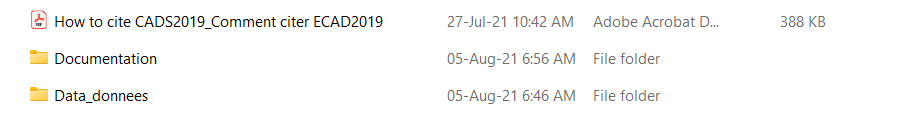
\includegraphics[width=0.9\linewidth,height=\textheight,keepaspectratio]{references/data-sources/../../assets/images/data5/cads7.png}
\end{center}

\subsection*{Data Documentation}\label{data-documentation}
\addcontentsline{toc}{subsection}{Data Documentation}

The data documentation folder includes three sub-folders:
\texttt{Codebook\_Livre\ des\ codes}, \texttt{Guide}, and
\texttt{Questionnaires}.

\begin{center}
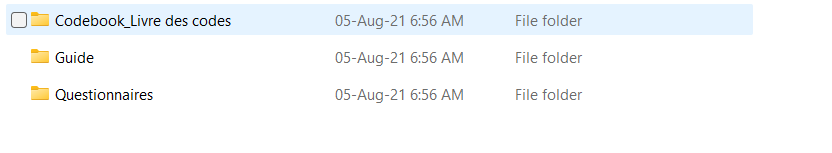
\includegraphics[width=0.9\linewidth,height=\textheight,keepaspectratio]{references/data-sources/../../assets/images/data5/cads8.png}
\end{center}

The \texttt{Guide} folder contains user guides (in English and French)
that provide an overview of the survey, including the methodology, data
collection process, data processing, data quality, and sampling weights.

\begin{center}
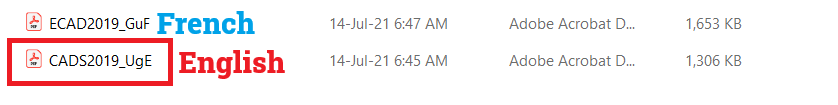
\includegraphics[width=0.9\linewidth,height=\textheight,keepaspectratio]{references/data-sources/../../assets/images/data5/cads9.png}
\end{center}

The \texttt{Codebook\_Livre\ des\ codes} folder contains codebooks (in
English and French) that provide detailed information about the
variables in the dataset, including variable names, labels, and values.
There are two types of codebooks: those with and those without variable
frequencies. But both codebooks provide the same information about the
variables in the dataset.

\begin{center}
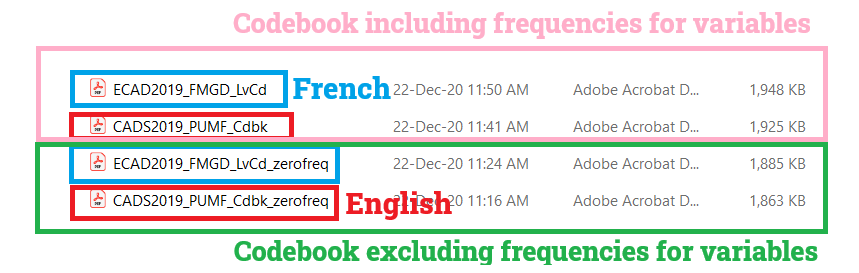
\includegraphics[width=0.9\linewidth,height=\textheight,keepaspectratio]{references/data-sources/../../assets/images/data5/cads10.png}
\end{center}

The \texttt{Questionnaires} folder contains the survey questionnaires
(in English and French) that were used to collect the data.

\subsection*{Data}\label{data-1}
\addcontentsline{toc}{subsection}{Data}

The \texttt{Data\_donnees} folder contains the dataset in CSV format.
You can open the dataset in Excel or any statistical software to explore
the data. The row represents the respondent, and the column represents
the variable:

\begin{center}
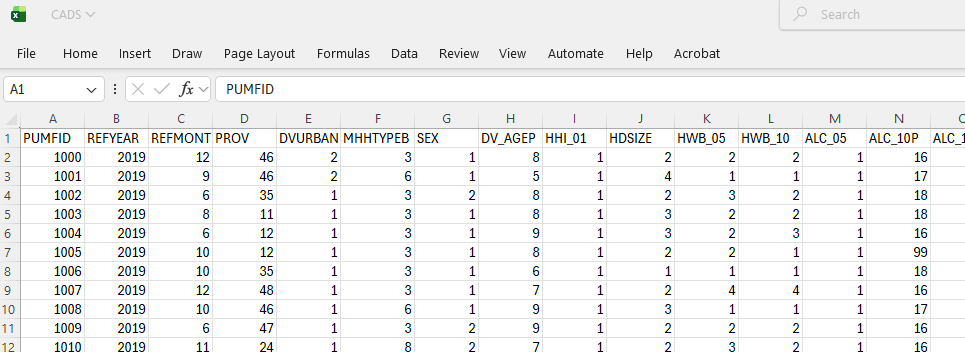
\includegraphics[width=0.9\linewidth,height=\textheight,keepaspectratio]{references/data-sources/../../assets/images/data5/cads11.png}
\end{center}

You can refer to the codebook to understand the variables that you are
interested in for your analysis. For example, if you are interested in
the variable \texttt{DVURBAN}, you can refer to the codebook to find out
that the variable (e.g., for the English version of the codebook with
frequencies):

\begin{center}
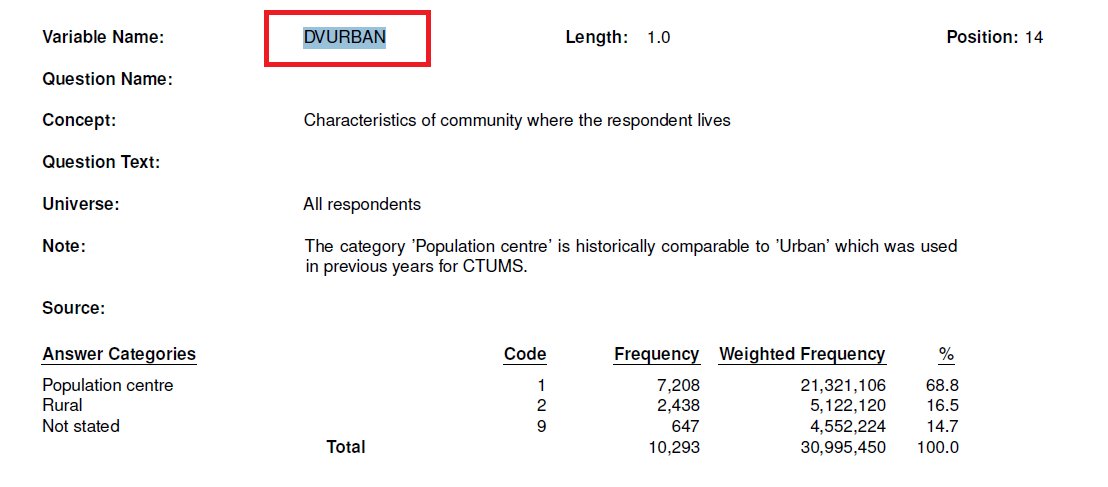
\includegraphics[width=0.9\linewidth,height=\textheight,keepaspectratio]{references/data-sources/../../assets/images/data5/cads12.png}
\end{center}

\chapter*{Data Source: CTNS}\label{data-source-ctns}
\addcontentsline{toc}{chapter}{Data Source: CTNS}

\markboth{Data Source: CTNS}{Data Source: CTNS}

The Canadian Tobacco and Nicotine Survey (CTNS) is a cross-sectional
survey that collects information on tobacco and nicotine use among
Canadians aged 15 years and older. The survey is conducted by Statistics
Canada on behalf of Health Canada and provides valuable insights into
the prevalence of cigarette smoking, vaping, cannabis, and alcohol use.

\begin{center}

\includegraphics[width=0.9\linewidth,height=\textheight,keepaspectratio]{references/data-sources/../../assets/images/data6/ctns1.png}
\end{center}

\marginnote{\begin{footnotesize}

\href{https://open.canada.ca/data/en/dataset/7147c035-4418-499c-9623-a0584debfcb1}{Health
Canada website for CTNS}

\end{footnotesize}}

\marginnote{\begin{footnotesize}

\href{https://www.canada.ca/en/health-canada/services/canadian-tobacco-nicotine-survey/2022-summary.html}{CTNS
2022 summary of results}

\end{footnotesize}}

\subsection*{Open Licence}\label{open-licence-2}
\addcontentsline{toc}{subsection}{Open Licence}

The CTNS is licensed under the
\href{https://open.canada.ca/en/open-government-licence-canada}{Open
Government Licence - Canada}. This means that the data can be freely
used, modified, and shared by anyone for any purpose, as long as they
provide proper attribution to the source of the data.

\subsection*{Data and Resources}\label{data-and-resources-2}
\addcontentsline{toc}{subsection}{Data and Resources}

The \texttt{Data\ and\ Resources} tab provides access to the public use
data, user guides, and the data dictionary.

\begin{center}
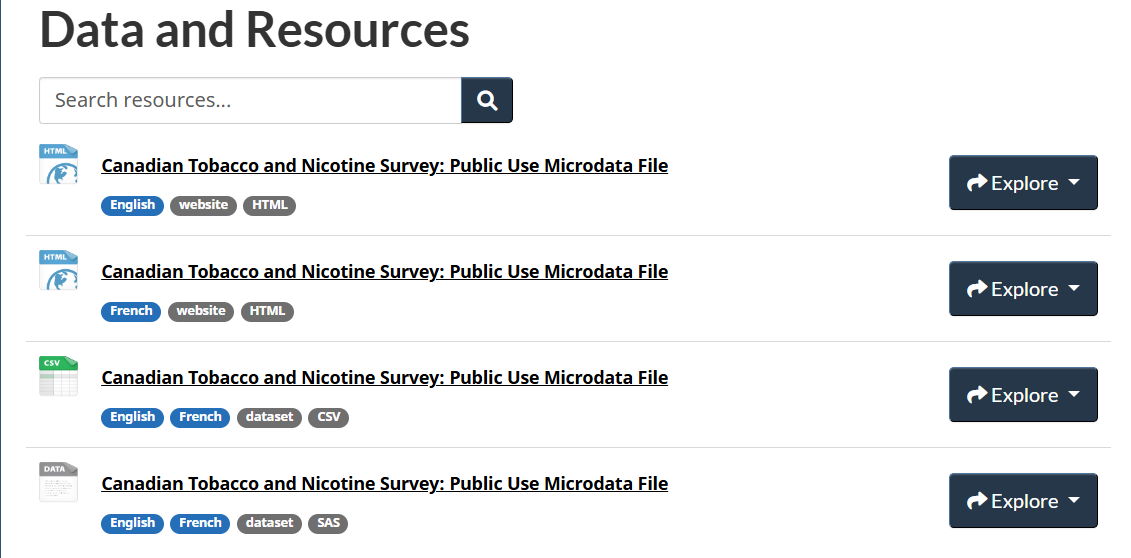
\includegraphics[width=0.9\linewidth,height=\textheight,keepaspectratio]{references/data-sources/../../assets/images/data6/ctns2.png}
\end{center}

The public use data file is available in a ZIP format. You can click on
the
\texttt{Canadian\ Tobacco\ and\ Nicotine\ Survey:\ Public\ Use\ Microdata\ File}
link, followed by \texttt{Go\ to\ resource} link to download the ZIP
file.

\begin{center}
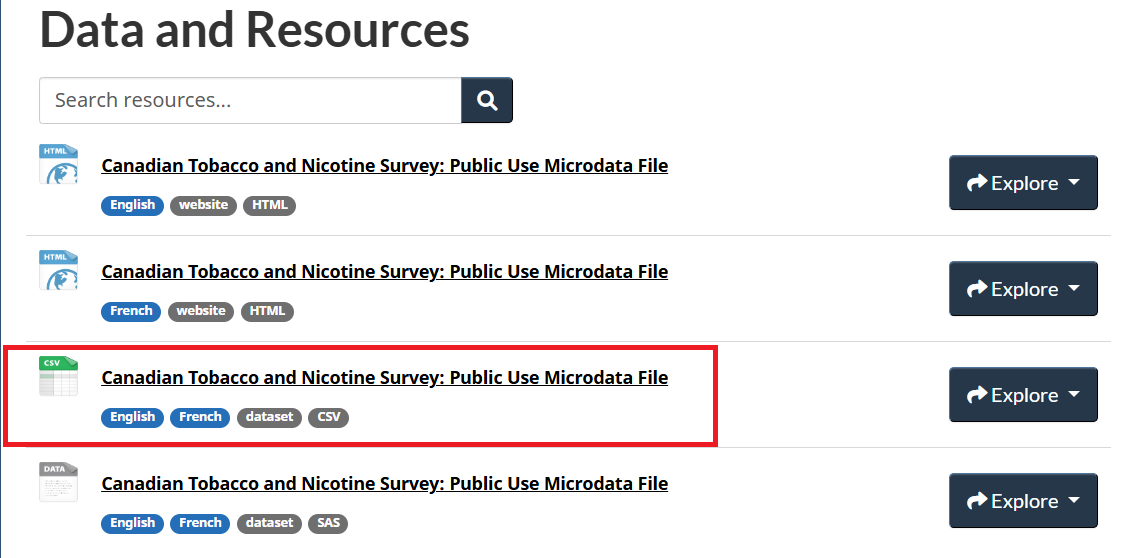
\includegraphics[width=0.9\linewidth,height=\textheight,keepaspectratio]{references/data-sources/../../assets/images/data6/ctns3.png}
\end{center}

\begin{center}

\includegraphics[width=0.9\linewidth,height=\textheight,keepaspectratio]{references/data-sources/../../assets/images/data6/ctns4.png}
\end{center}

Similar to the \href{data5.html}{Canadian Alcohol and Drugs Survey
(CADS)} tutorial, the ZIP file for CTNS contains the following files:
citation instructions, data documentation, and the dataset in CSV
format. The data documentation, questionnaire, and codebook are also the
same as those for CADS. The only difference is that the data
documentation and questionnaire for CTNS are labelled \texttt{CTNS}
rather than \texttt{CADS}.

\chapter*{Data Source: CSADS}\label{data-source-csads}
\addcontentsline{toc}{chapter}{Data Source: CSADS}

\markboth{Data Source: CSADS}{Data Source: CSADS}

The Canadian Student Alcohol and Drugs Survey (CSADS) is a national
survey that collects data on the alcohol and drug use patterns of
Canadian students in grades 7 to 12. The survey is conducted every two
years and provides valuable insights into the prevalence and trends of
substance use among Canadian youth.

\begin{center}

\includegraphics[width=0.9\linewidth,height=\textheight,keepaspectratio]{references/data-sources/../../assets/images/data7/csads1.png}
\end{center}

\marginnote{\begin{footnotesize}

\href{https://open.canada.ca/data/en/dataset/7147c035-4418-499c-9623-a0584debfcb1}{Health
Canada website for CTNS}

\end{footnotesize}}

\marginnote{\begin{footnotesize}

\href{https://www.canada.ca/en/health-canada/services/canadian-student-tobacco-alcohol-drugs-survey.html}{CSADS
summary of results}

\end{footnotesize}}

\subsection*{Open Licence}\label{open-licence-3}
\addcontentsline{toc}{subsection}{Open Licence}

The CTNS is licensed under the
\href{https://open.canada.ca/en/open-government-licence-canada}{Open
Government Licence - Canada}. This means that the data can be freely
used, modified, and shared by anyone for any purpose, as long as they
provide proper attribution to the source of the data.

\subsection*{Data and Resources}\label{data-and-resources-3}
\addcontentsline{toc}{subsection}{Data and Resources}

The \texttt{Data\ and\ Resources} tab provides access to the public use
data, user guides, the data dictionary, and information on bootstrap
weights.

\begin{center}
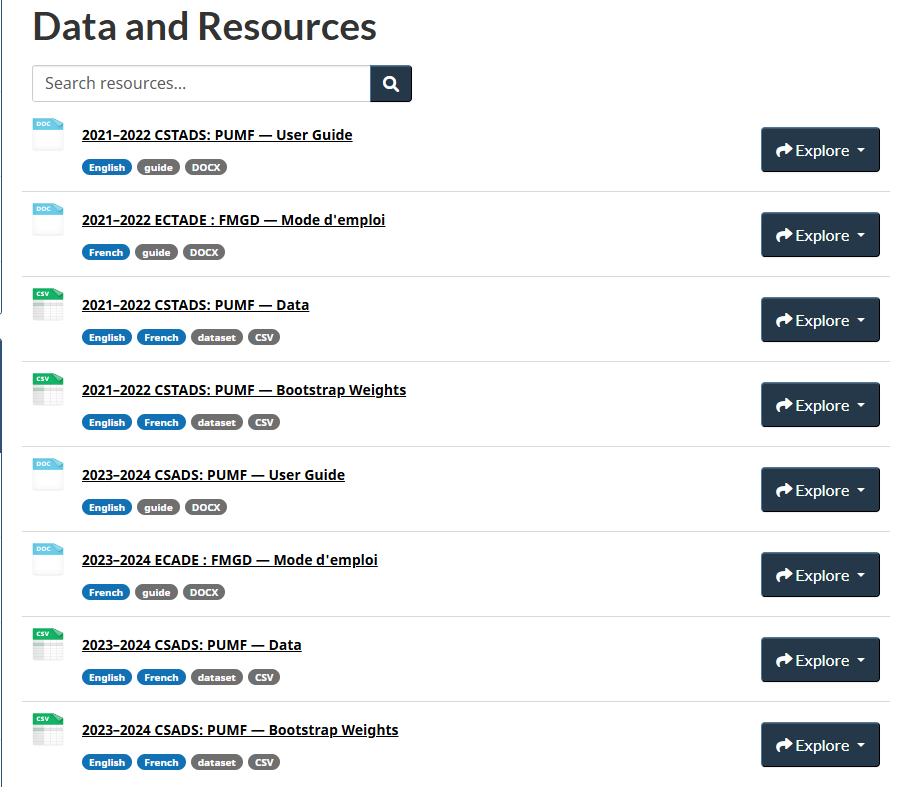
\includegraphics[width=0.9\linewidth,height=\textheight,keepaspectratio]{references/data-sources/../../assets/images/data7/csads2.png}
\end{center}

To download the 2021--2022 CSTADS, you can click on the
\texttt{2021–2022\ CSTADS:\ PUMF\ —\ Dataset\ in\ CSV\ format} link. The
data is available to download in various formats. Under the
\texttt{Download} tab, you can find the formats. For example, you can
download the data in CSV format by clicking on the \texttt{CSV} link:

\begin{center}
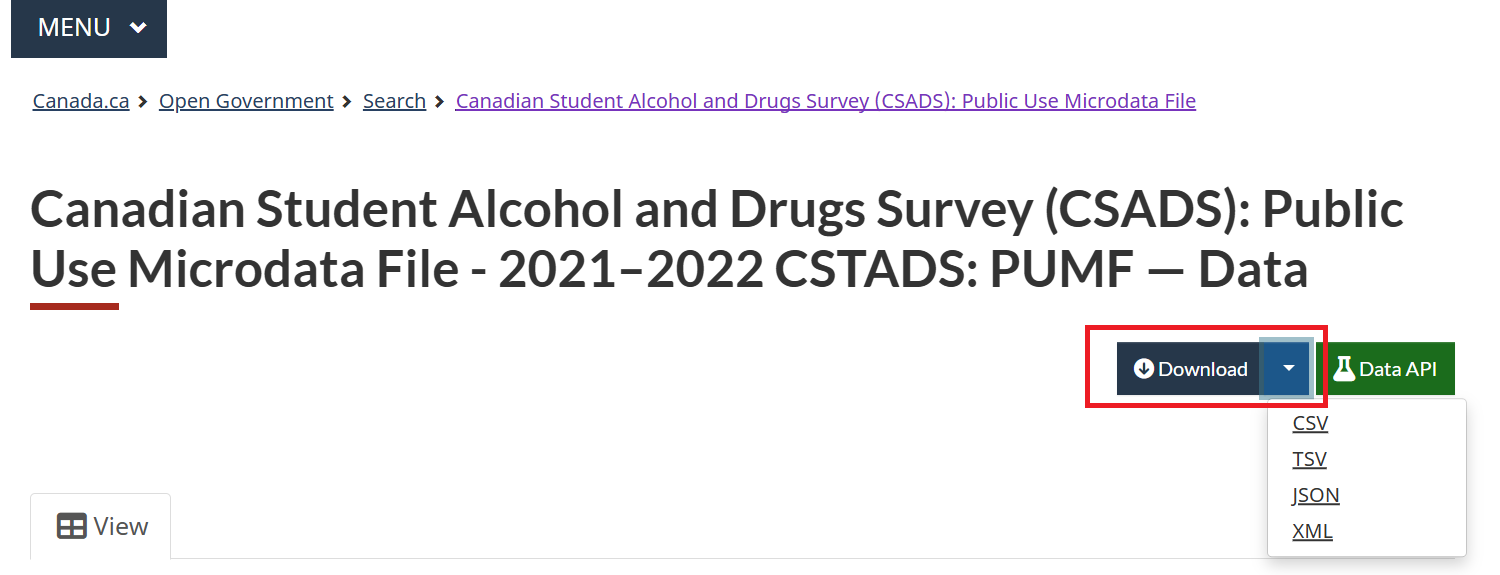
\includegraphics[width=0.9\linewidth,height=\textheight,keepaspectratio]{references/data-sources/../../assets/images/data7/csads3.png}
\end{center}

After downloading, you can open the data in Excel, Google Sheets, or any
statistical software. The data is structured in a tabular format, with
each row representing an individual respondent and each column
representing different variables:

\begin{center}
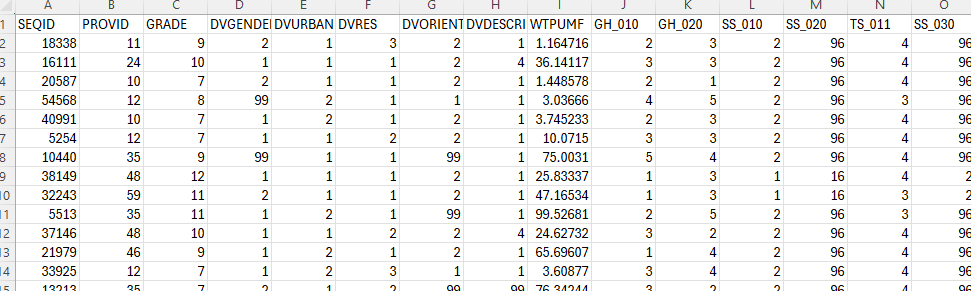
\includegraphics[width=0.9\linewidth,height=\textheight,keepaspectratio]{references/data-sources/../../assets/images/data7/csads4.png}
\end{center}

The user guide gives detailed information on the survey methodology,
data collection process, and how to use the public use microdata file
(PUMF). You can also find the variable names and their descriptions in
this \texttt{DOCX} file.

\begin{center}
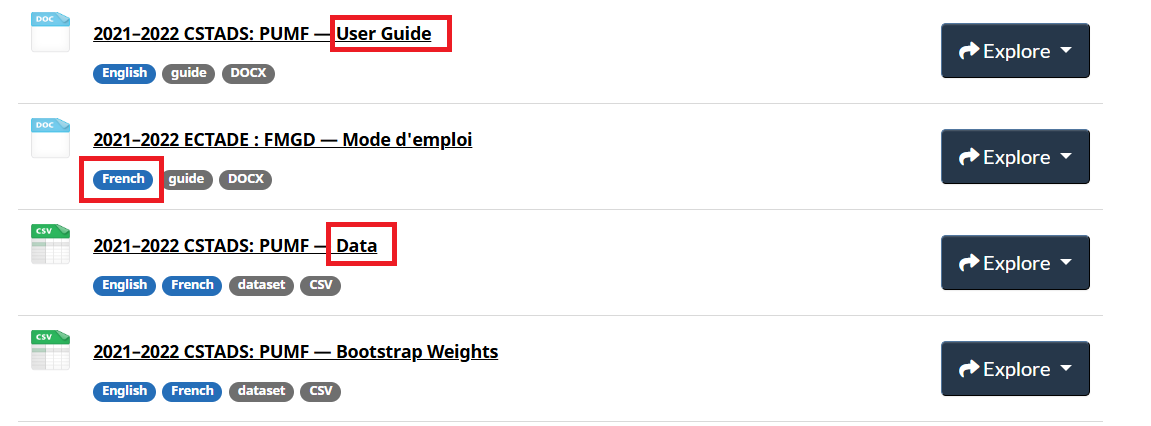
\includegraphics[width=0.9\linewidth,height=\textheight,keepaspectratio]{references/data-sources/../../assets/images/data7/csads5.png}
\end{center}

\begin{center}

\includegraphics[width=0.9\linewidth,height=\textheight,keepaspectratio]{references/data-sources/../../assets/images/data7/csads6.png}
\end{center}

\begin{center}

\includegraphics[width=0.9\linewidth,height=\textheight,keepaspectratio]{references/data-sources/../../assets/images/data7/csads7.png}
\end{center}

To find a variable description, you are referred to the
\texttt{User\ Guide}. For example, the variable \texttt{GH\_010} is
described as follows:

\begin{center}
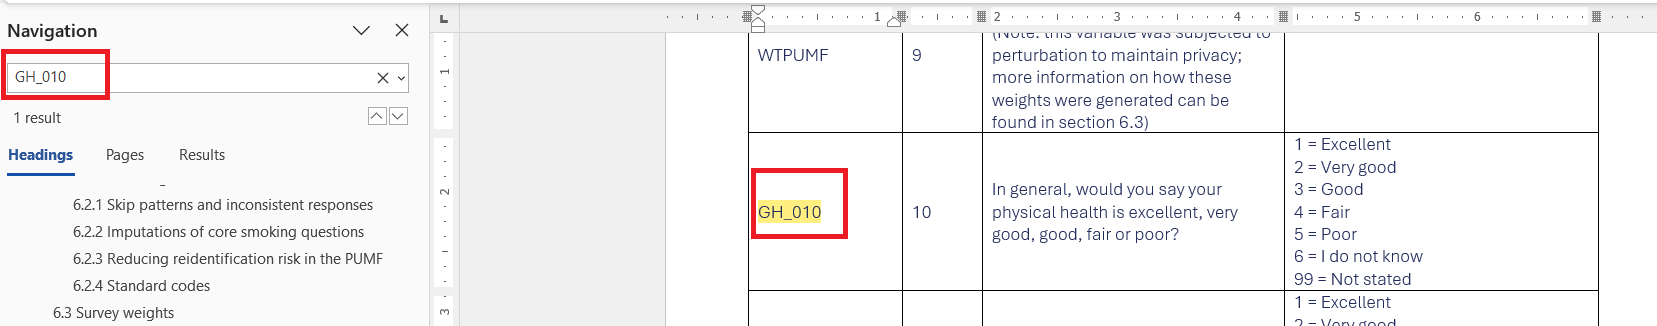
\includegraphics[width=0.9\linewidth,height=\textheight,keepaspectratio]{references/data-sources/../../assets/images/data7/csads8.png}
\end{center}

\chapter*{Data Source: PHAC Health
Infobase}\label{data-source-phac-health-infobase}
\addcontentsline{toc}{chapter}{Data Source: PHAC Health Infobase}

\markboth{Data Source: PHAC Health Infobase}{Data Source: PHAC Health
Infobase}

The Health Infobase is a comprehensive digital platform maintained by
the Public Health Agency of Canada (PHAC). The Infobase provides access
to a wide range of health-related data tools, infographics, charts and
blogs. There are 182 data sources available on the Infobase. The Health
Infobase serves as a central hub for national surveillance data,
interactive data tools, and public health reports. The platform is
frequently updated with the latest surveillance data.

\begin{center}
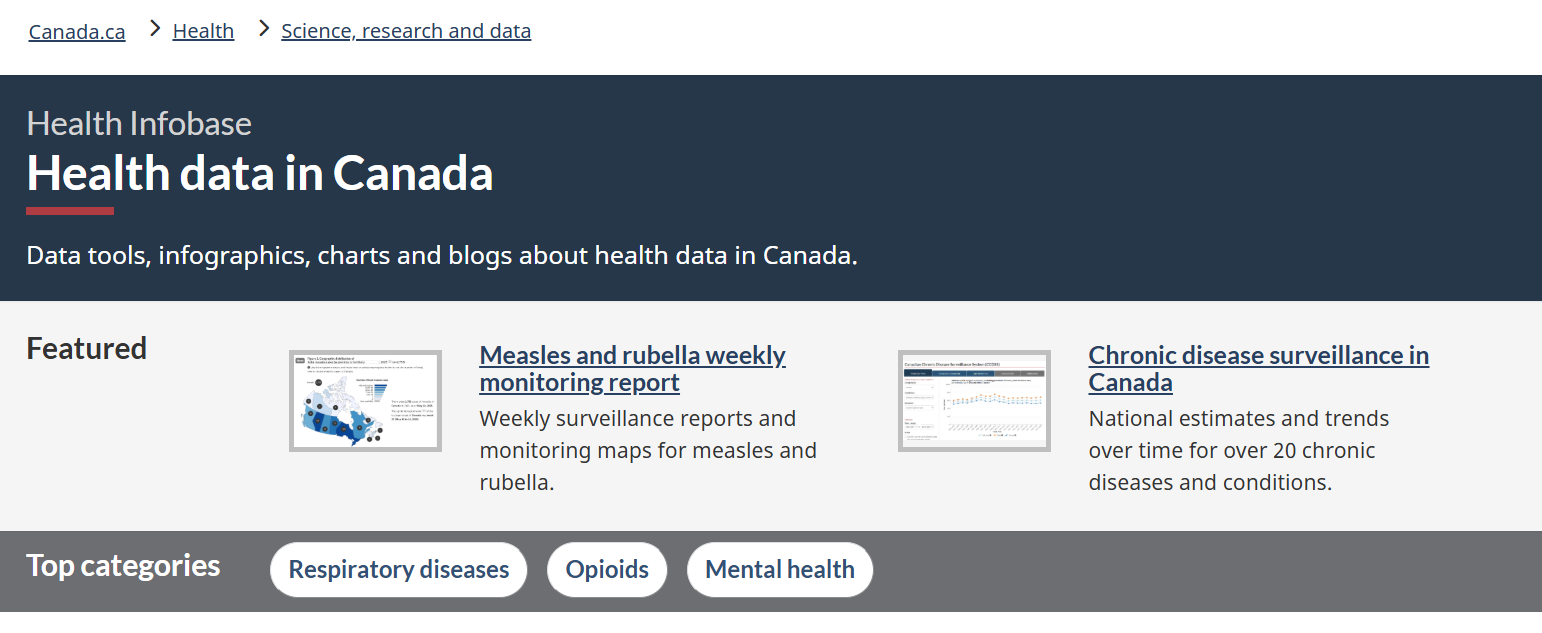
\includegraphics[width=0.9\linewidth,height=\textheight,keepaspectratio]{references/data-sources/../../assets/images/data8/infobase1.png}
\end{center}

\marginnote{\begin{footnotesize}

\href{https://health-infobase.canada.ca/}{PHAC Health Infobase}

\end{footnotesize}}

\subsection*{Data Categories}\label{data-categories}
\addcontentsline{toc}{subsection}{Data Categories}

The Infobase provides access to health data under six categories:

\begin{itemize}
\item
  \texttt{Diseases\ and\ disorders}: Comprehensive tracking of chronic
  conditions such as cancer, cardiovascular diseases, and COVID-19.
\item
  \texttt{Drugs\ and\ vaccines}: Data on prescription drugs, vaccine
  coverage, and immunization rates across the country. `
\item
  \texttt{Mental\ health,\ healthy\ living\ and\ environment}:
  Information on mental health indicators, physical activity levels,
  nutrition, and environmental factors such as wildfires.
\item
  \texttt{Injuries\ and\ death}: Data on death, suicide, violence, and
  drowning across regions.
\item
  \texttt{Population\ groups\ and\ demography}: Data on birth,
  maternity, children, family, and disabilities.
\item
  \texttt{Substance\ use}: Data on substance use such as alcohol,
  cannabis use, opioids, and smoking.
\end{itemize}

Under each category, users can select the data for specific health
topics. The three top categories are \texttt{Respiratory\ diseases},
\texttt{Opioids} and \texttt{Mental\ health}.

\begin{center}
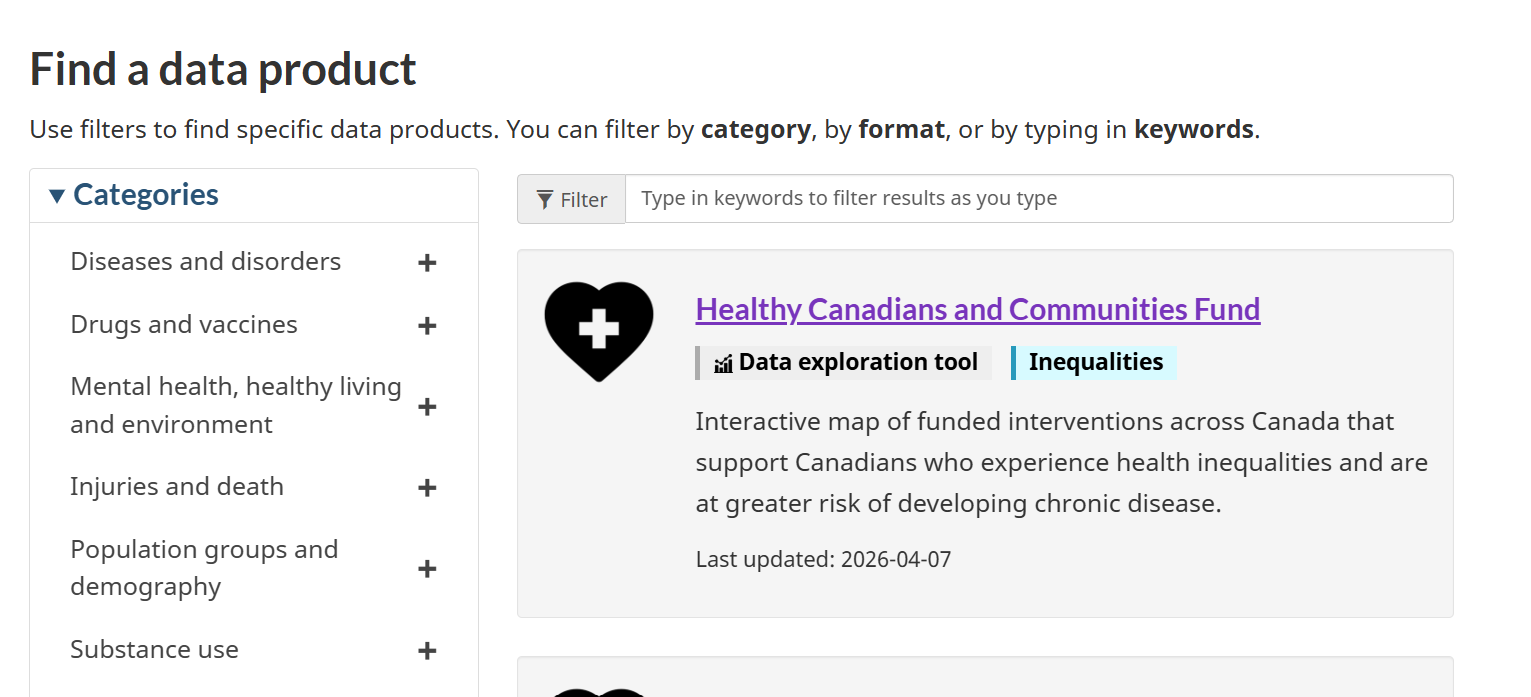
\includegraphics[width=0.9\linewidth,height=\textheight,keepaspectratio]{references/data-sources/../../assets/images/data8/infobase2.png}
\end{center}

\begin{center}
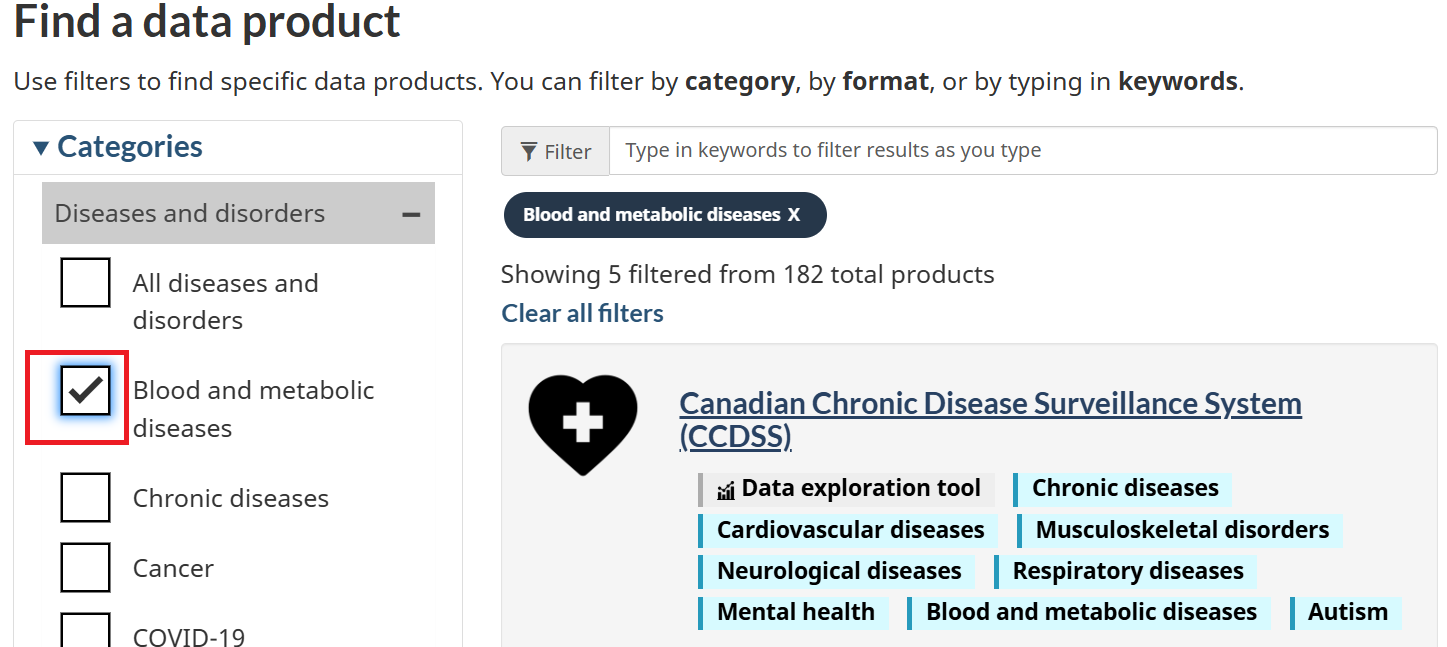
\includegraphics[width=0.9\linewidth,height=\textheight,keepaspectratio]{references/data-sources/../../assets/images/data8/infobase3.png}
\end{center}

You can filter the data by category, by format, or by typing in
keywords.

\begin{center}
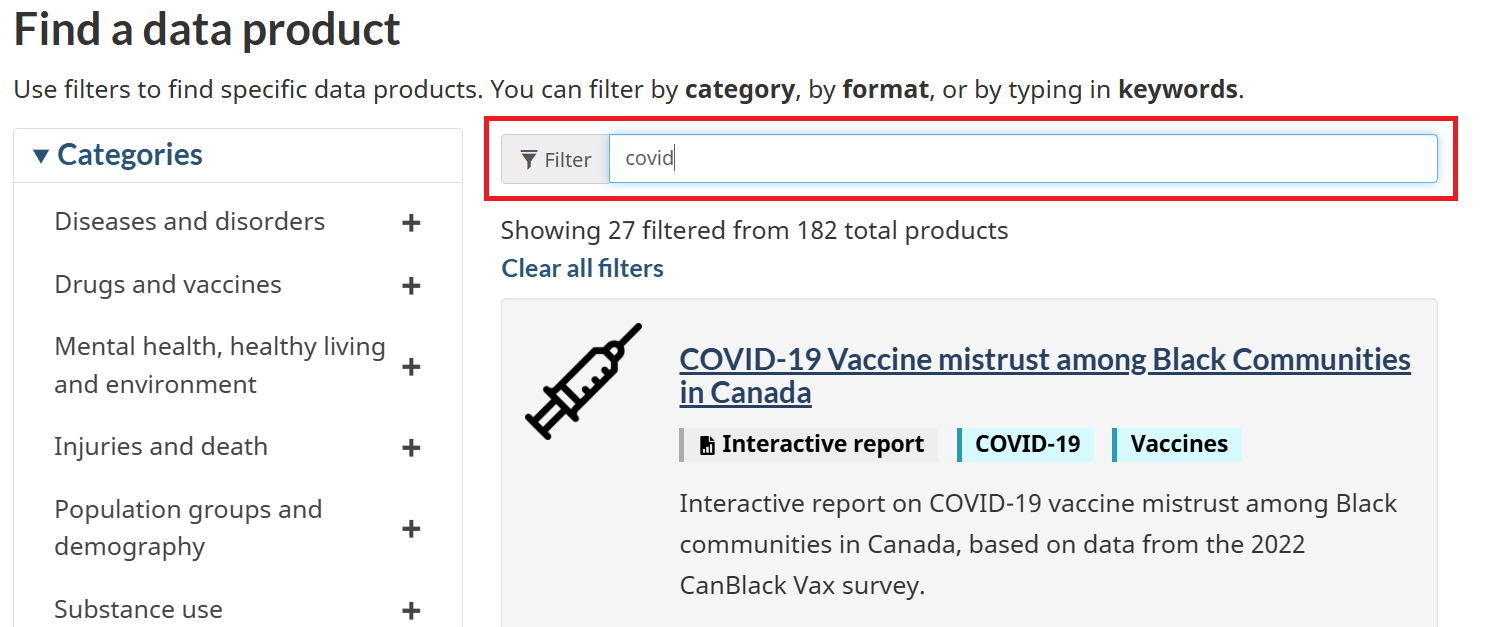
\includegraphics[width=0.9\linewidth,height=\textheight,keepaspectratio]{references/data-sources/../../assets/images/data8/infobase4.png}
\end{center}

You can also filter the data by type, such as blog, infographic, or
report.

\begin{center}
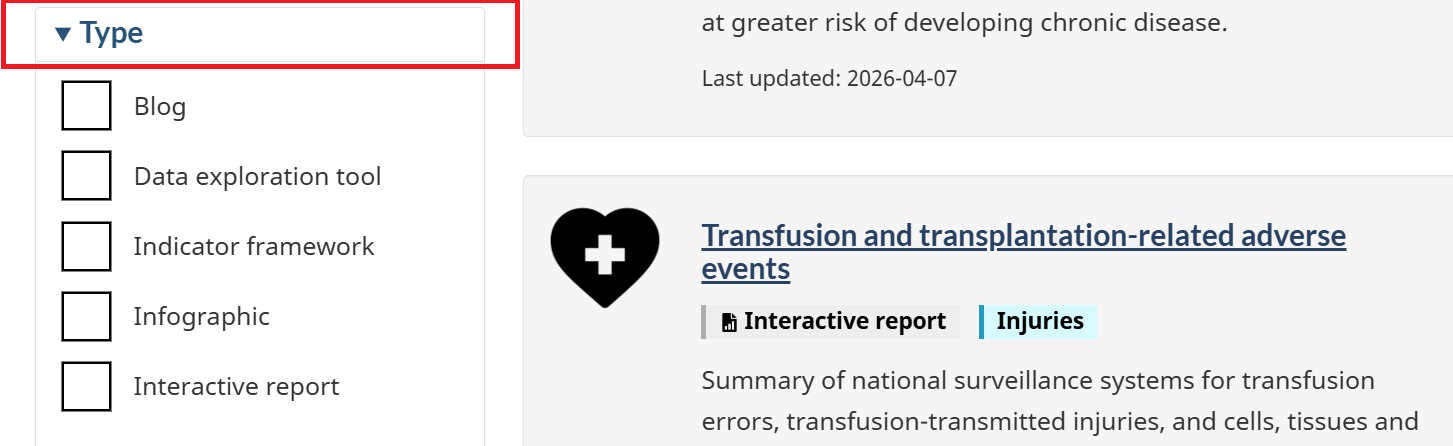
\includegraphics[width=0.9\linewidth,height=\textheight,keepaspectratio]{references/data-sources/../../assets/images/data8/infobase5.png}
\end{center}

\subsection*{Data Availability}\label{data-availability}
\addcontentsline{toc}{subsection}{Data Availability}

The level of information provided in the data sources varies. For some
data sources/products, you can find blogs, infographics, and reports
along with individual-level data. However, for some data
sources/products, you may only find the summary statistics without
individual-level data, i.e., only aggregated-level data. For example,
the \texttt{Human\ Papillomavirus\ Indicator\ Framework} product
provides quick statistics, data tools and a list of publications:

\begin{center}
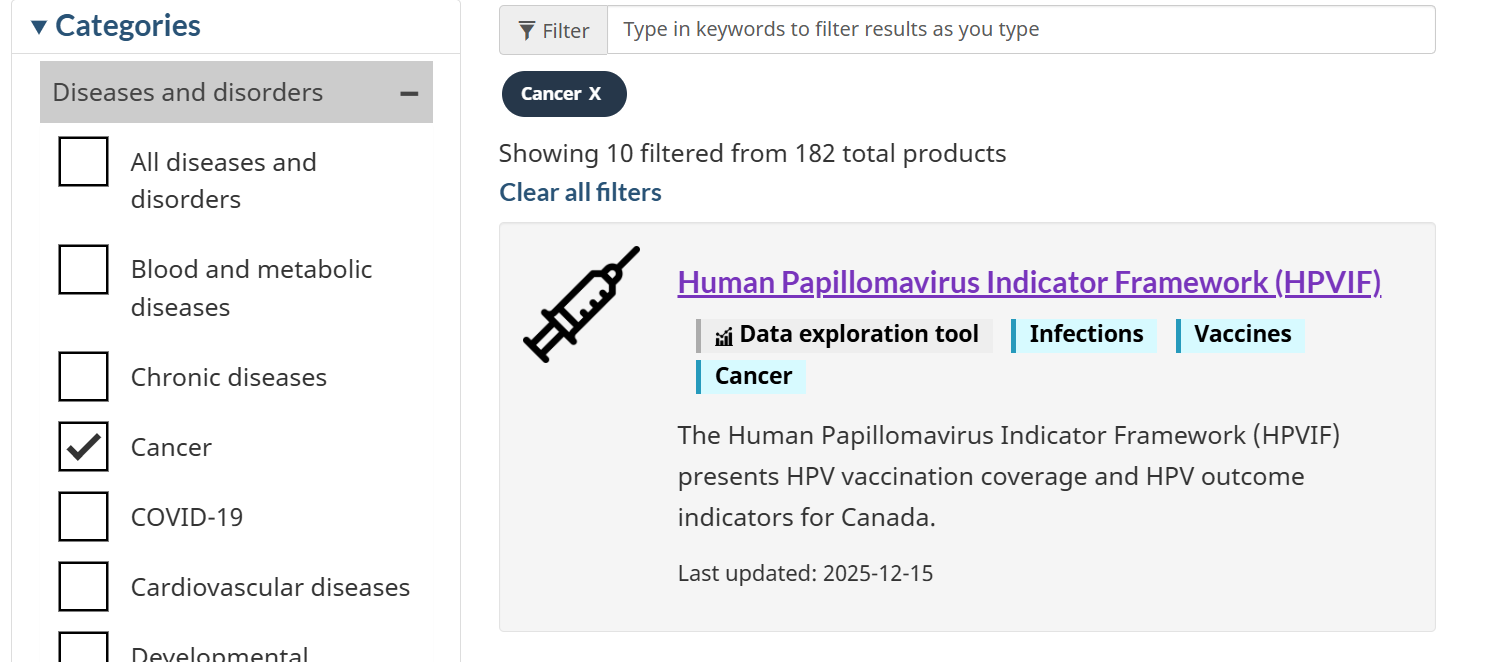
\includegraphics[width=0.9\linewidth,height=\textheight,keepaspectratio]{references/data-sources/../../assets/images/data8/infobase6.png}
\end{center}

\begin{center}
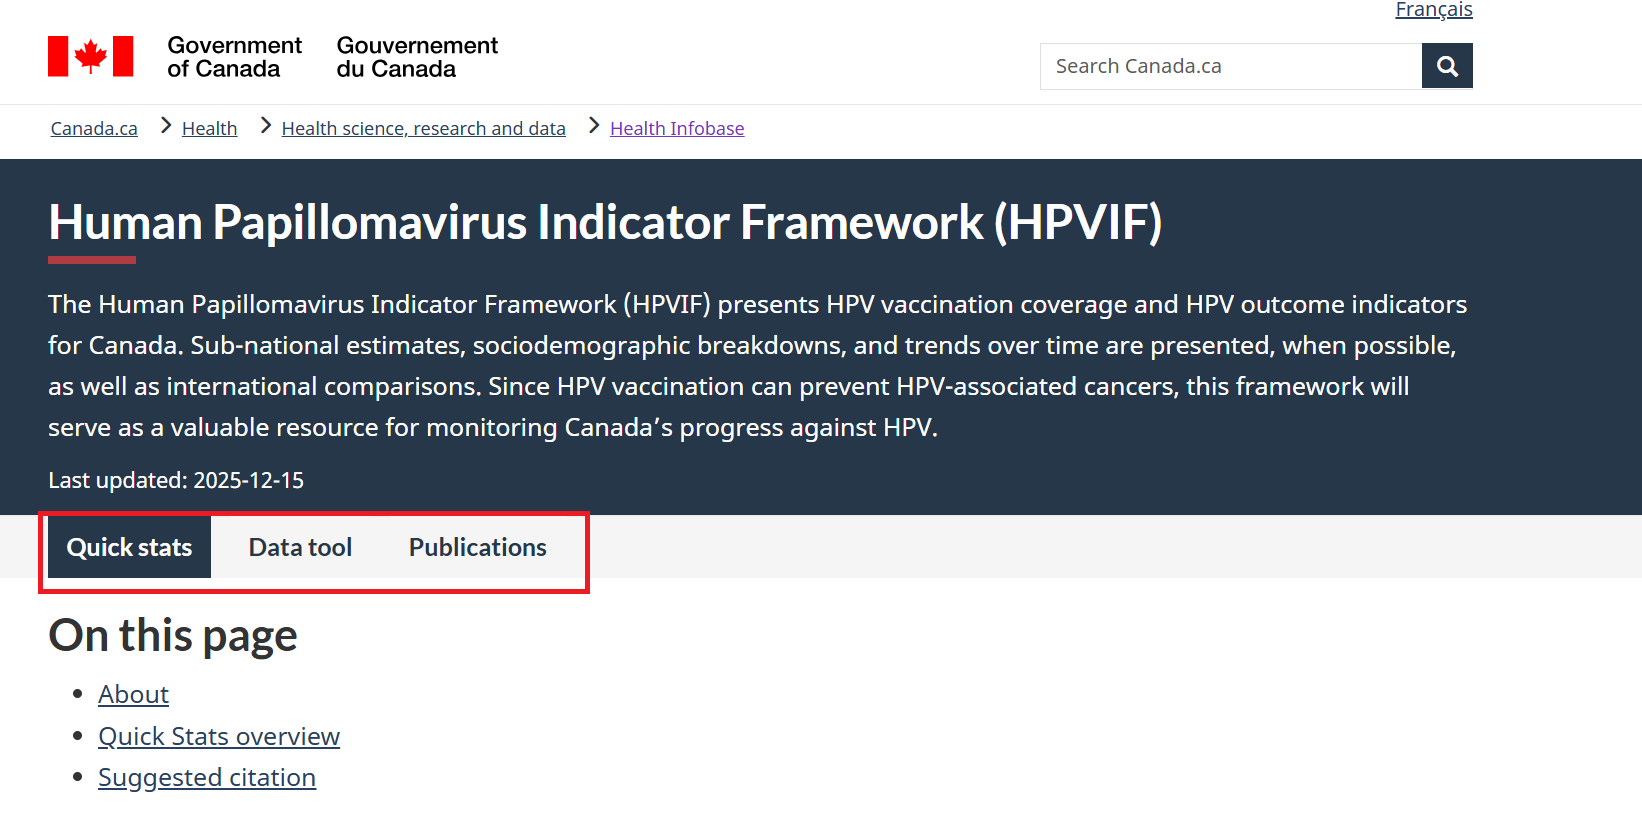
\includegraphics[width=0.9\linewidth,height=\textheight,keepaspectratio]{references/data-sources/../../assets/images/data8/infobase7.png}
\end{center}

The
\texttt{Drug\ and\ alcohol\ use\ in\ Canada:\ Postsecondary\ students}
product provides summary statistics as well as links to download data in
CSV format:

\begin{center}
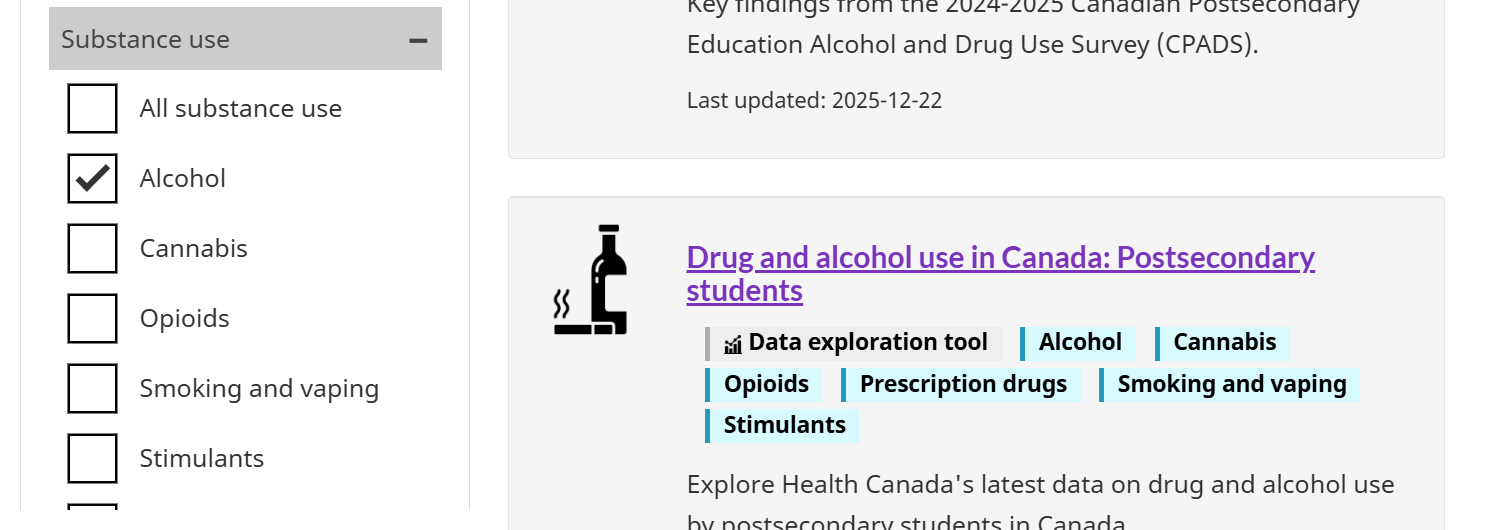
\includegraphics[width=0.9\linewidth,height=\textheight,keepaspectratio]{references/data-sources/../../assets/images/data8/infobase8.png}
\end{center}

\begin{center}
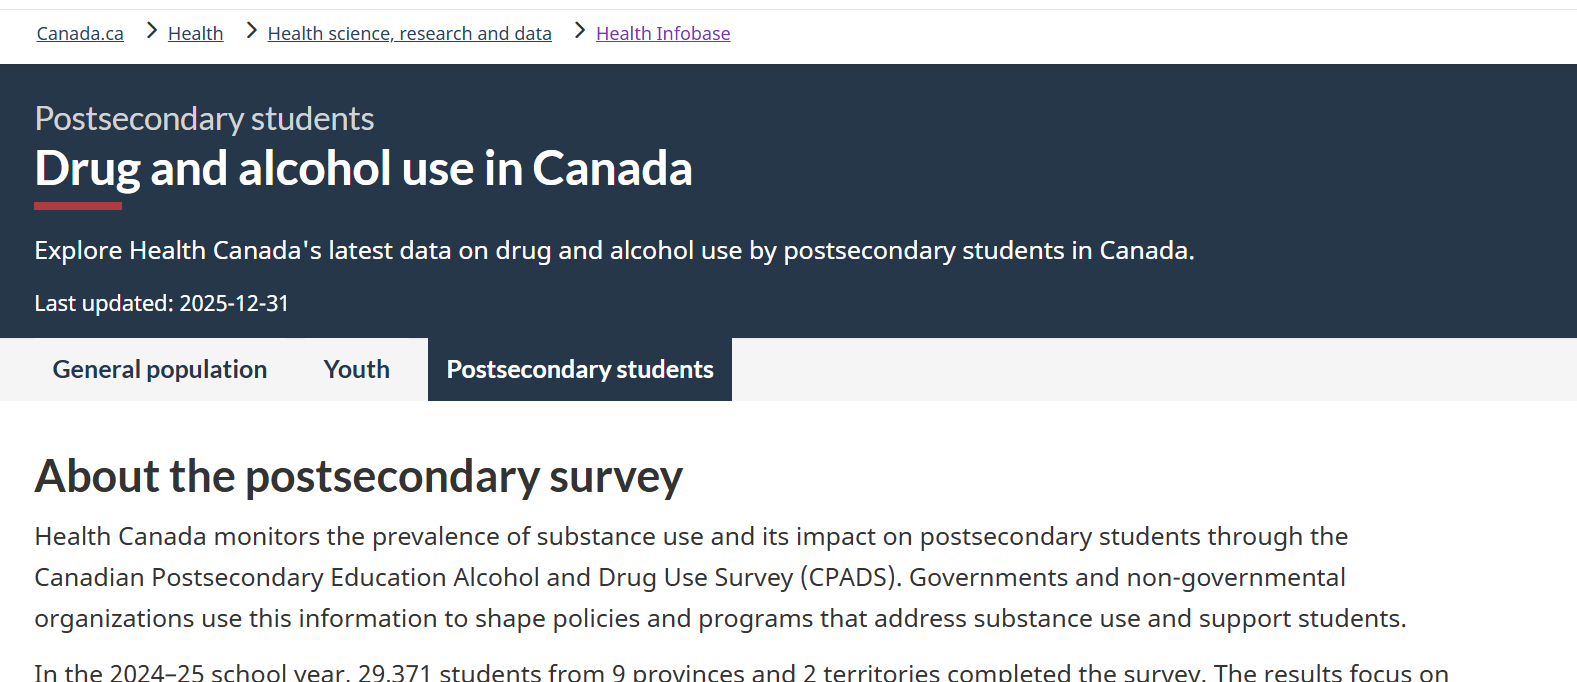
\includegraphics[width=0.9\linewidth,height=\textheight,keepaspectratio]{references/data-sources/../../assets/images/data8/infobase9.png}
\end{center}

\begin{center}
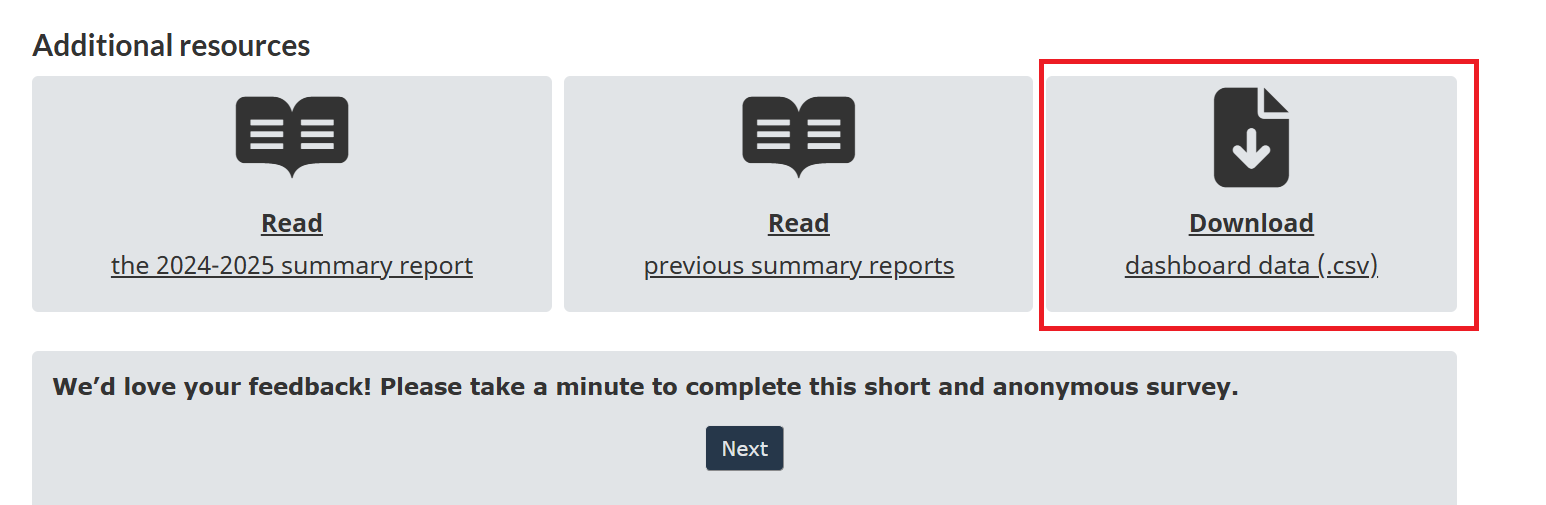
\includegraphics[width=0.9\linewidth,height=\textheight,keepaspectratio]{references/data-sources/../../assets/images/data8/infobase10.png}
\end{center}

\chapter*{Data Source: CCDSS}\label{data-source-ccdss}
\addcontentsline{toc}{chapter}{Data Source: CCDSS}

\markboth{Data Source: CCDSS}{Data Source: CCDSS}

The Canadian Chronic Disease Surveillance System (CCDSS) is a
collaborative network of provincial and territorial chronic disease
surveillance systems in Canada. The CCDSS is supported by the Public
Health Agency of Canada (PHAC) and provincial/territorial governments.
The CCDSS was established to provide the estimates of the prevalence and
incidence of chronic diseases in Canada, as well as to monitor trends
over time for more than 20 chronic diseases to help inform health
policies and resource planning. The CCDSS is part of the PHAC Health
Infobase that we covered in the previous tutorial on
\href{data8.html}{Health Infobase}. The CCDSS uses health administrative
data, such as hospital discharge records, physician billing claims, and
prescription drug data.

\begin{center}
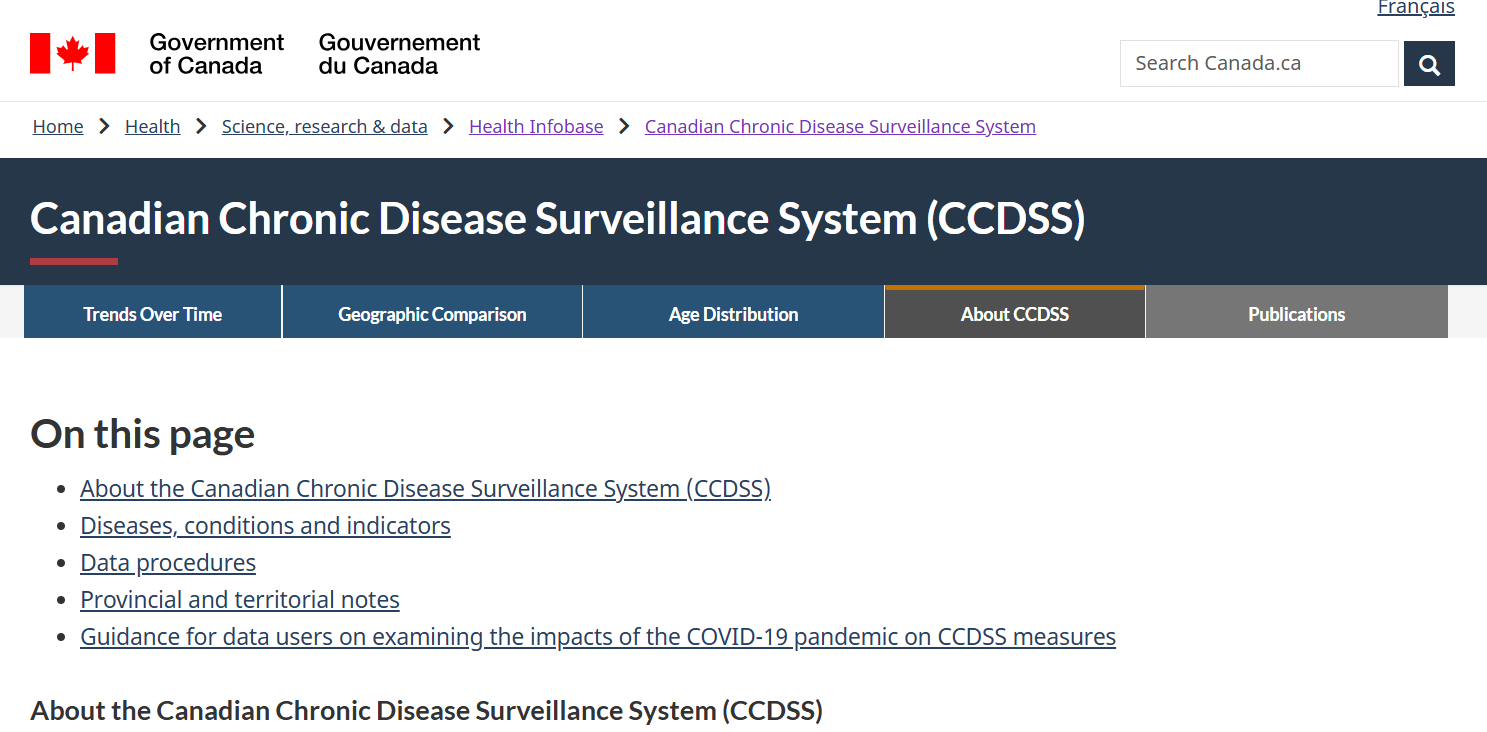
\includegraphics[width=0.9\linewidth,height=\textheight,keepaspectratio]{references/data-sources/../../assets/images/data9/ccdss1.png}
\end{center}

\marginnote{\begin{footnotesize}

\href{https://health-infobase.canada.ca/ccdss/}{CCDSS website}

\end{footnotesize}}

\subsection*{Key Indicator Categories}\label{key-indicator-categories}
\addcontentsline{toc}{subsection}{Key Indicator Categories}

The CCDSS website provides a variety of indicators related to chronic
diseases, such as autism, cardiovascular diseases, chronic respiratory
diseases, diabetes, mental health disorders, musculoskeletal disorders,
neurological disorders, and multimorbidity.

\begin{center}
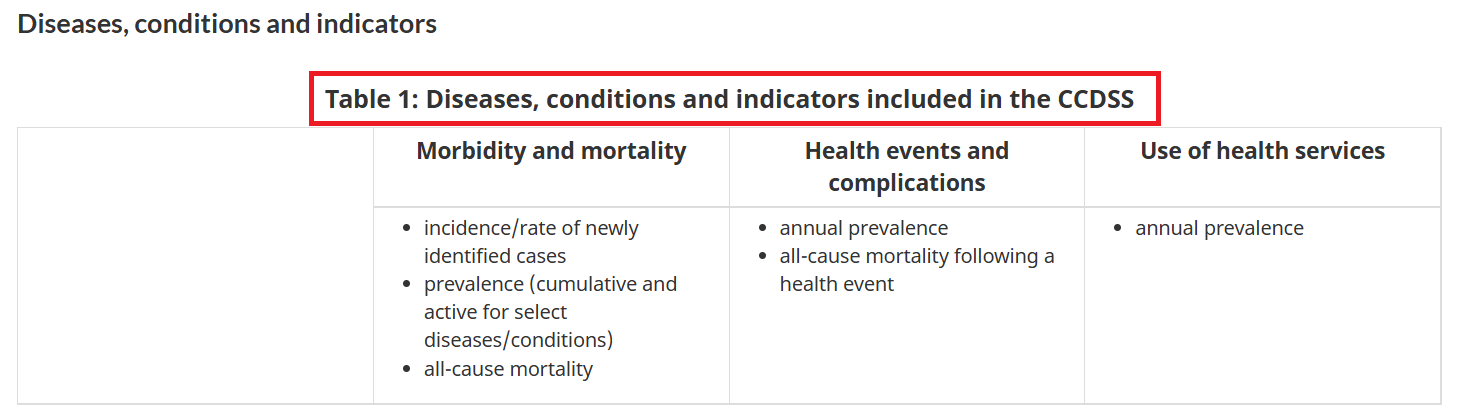
\includegraphics[width=0.9\linewidth,height=\textheight,keepaspectratio]{references/data-sources/../../assets/images/data9/ccdss2.png}
\end{center}

\begin{center}
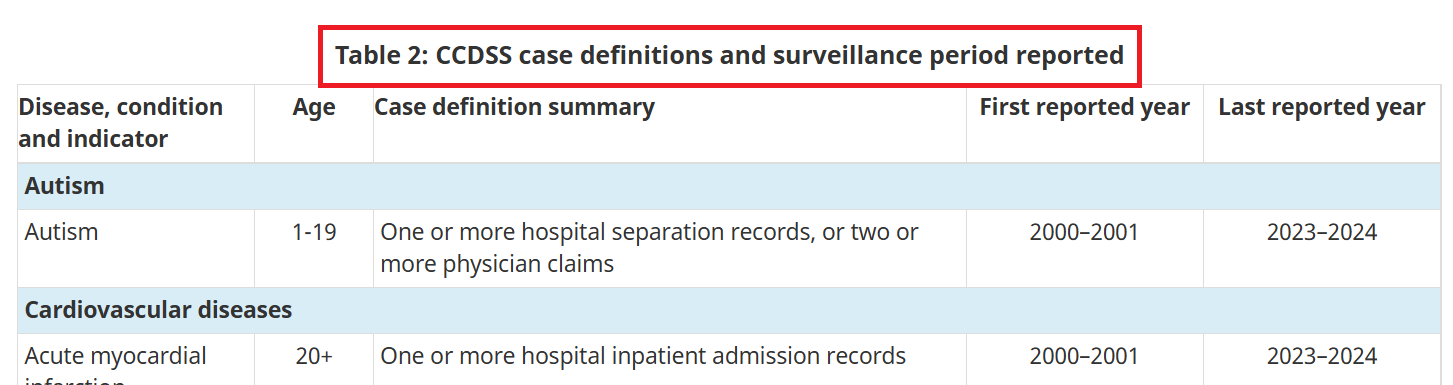
\includegraphics[width=0.9\linewidth,height=\textheight,keepaspectratio]{references/data-sources/../../assets/images/data9/ccdss3.png}
\end{center}

\subsection*{Data Tool}\label{data-tool}
\addcontentsline{toc}{subsection}{Data Tool}

The CCDSS website provides a data tool that allows users to explore and
visualize the data on chronic diseases in Canada. The data tool provides
interactive charts and tables that allow users to explore the data by
province/territory.

\begin{center}
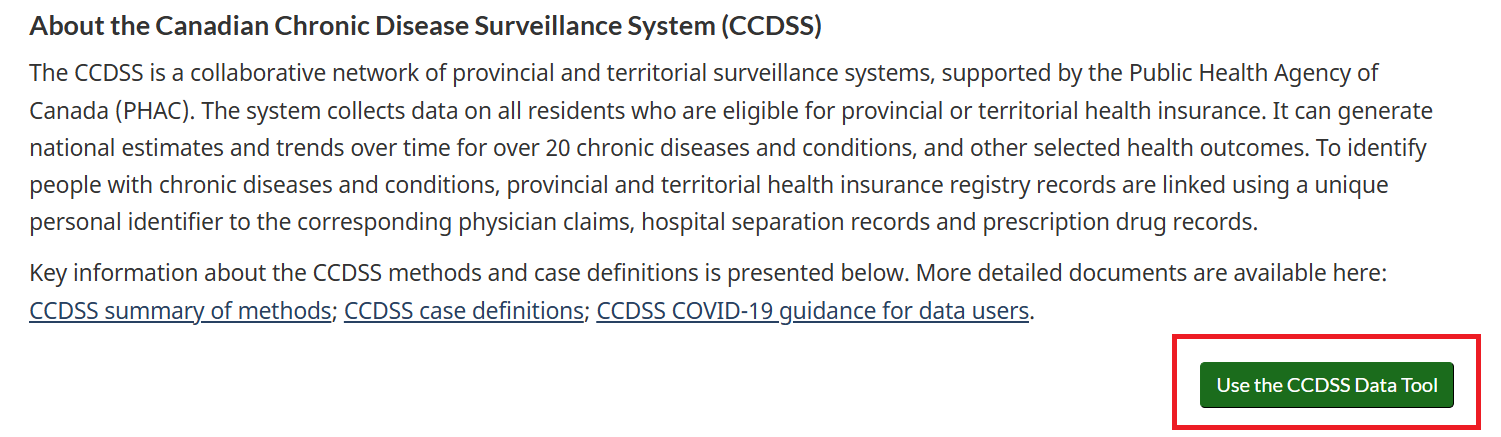
\includegraphics[width=0.9\linewidth,height=\textheight,keepaspectratio]{references/data-sources/../../assets/images/data9/ccdss4.png}
\end{center}

\marginnote{\begin{footnotesize}

\href{https://health-infobase.canada.ca/ccdss/data-tool/Index}{CCDSS
Data Tool}

\end{footnotesize}}

Users can use the data tool to explore the prevalence and incidence of
cases, mortality rates, and health service utilization, and to track
individuals living with two or more chronic conditions.

\begin{center}
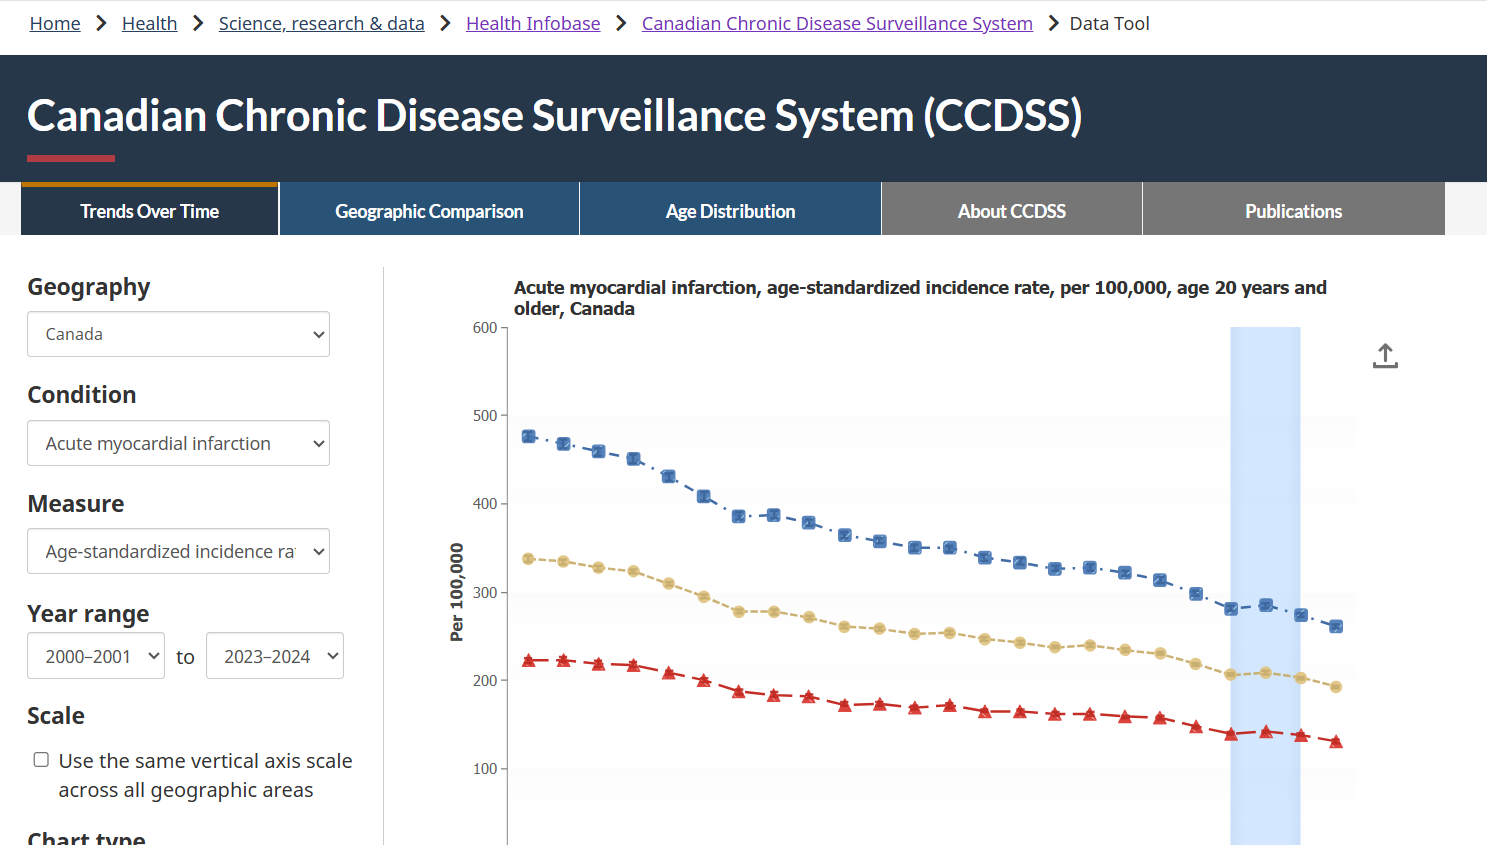
\includegraphics[width=0.9\linewidth,height=\textheight,keepaspectratio]{references/data-sources/../../assets/images/data9/ccdss5.png}
\end{center}

Users can explore trends over time, compare data across
provinces/territories, and view the distribution of cases by age group.
Under the \texttt{Publication} tab, you can find information on the
repository for data-driven insights, fact sheets, peer-reviewed
publications, and reports.

\begin{center}
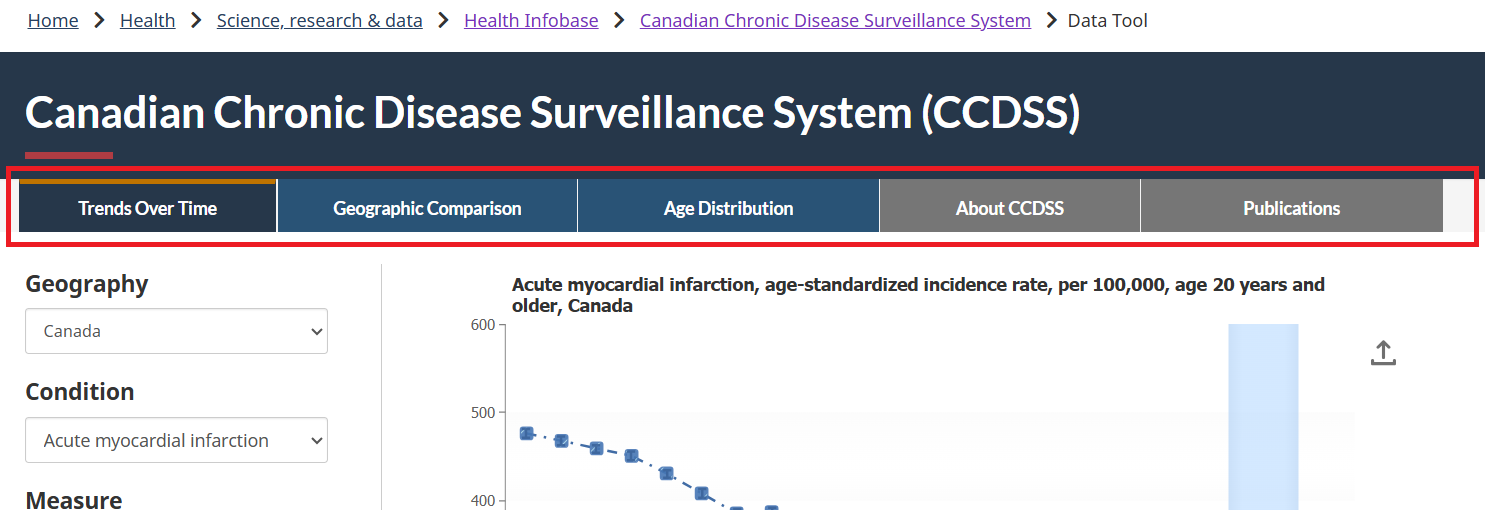
\includegraphics[width=0.9\linewidth,height=\textheight,keepaspectratio]{references/data-sources/../../assets/images/data9/ccdss6.png}
\end{center}

\subsection*{Interactive chart example}\label{interactive-chart-example}
\addcontentsline{toc}{subsection}{Interactive chart example}

Consider \texttt{Asthma} under \texttt{Chronic\ respiratory\ diseases}
as an example.

\begin{center}
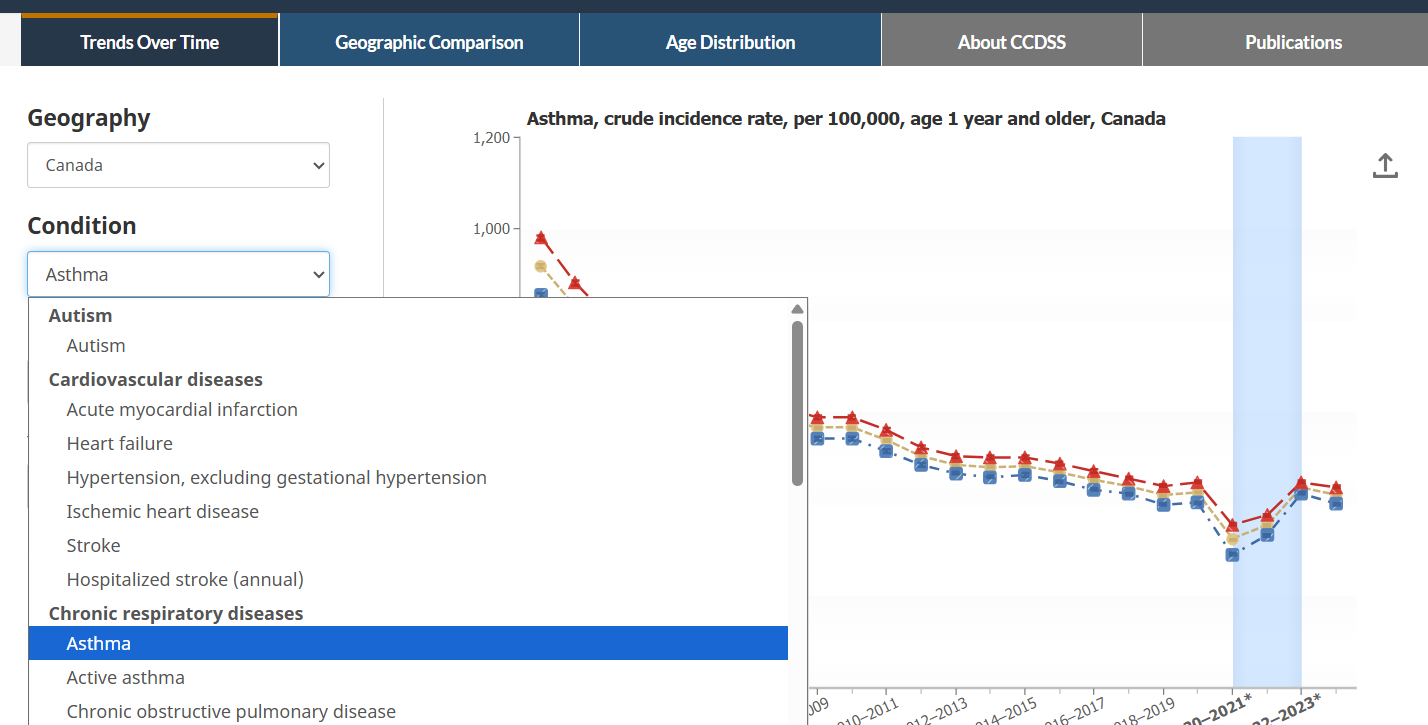
\includegraphics[width=0.9\linewidth,height=\textheight,keepaspectratio]{references/data-sources/../../assets/images/data9/ccdss7.png}
\end{center}

You can explore different summary measures by filtering by geography,
measure, and year. Again, you can further explore trends over time,
compare data across provinces/territories, and view the distribution of
cases by age group.

\begin{center}
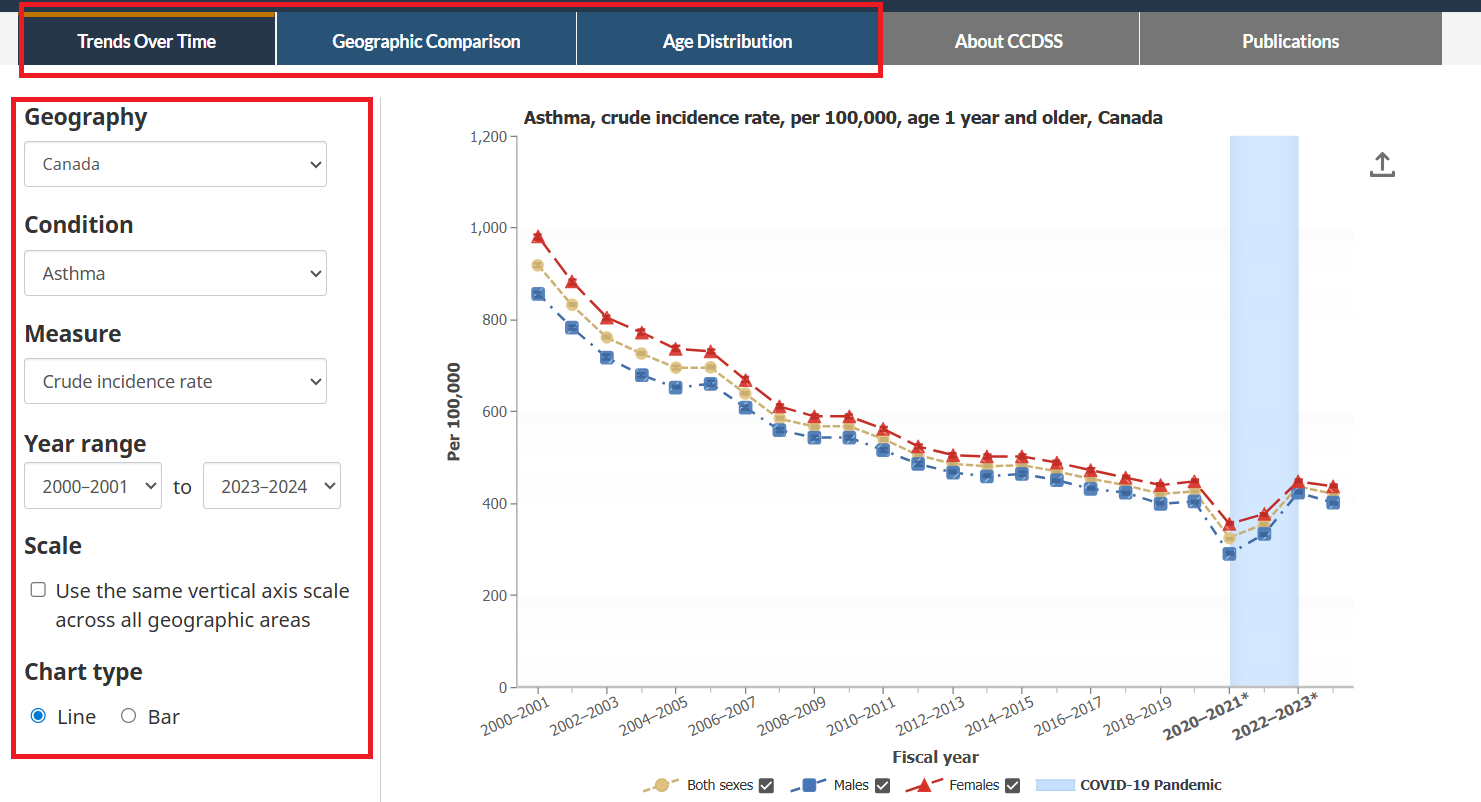
\includegraphics[width=0.9\linewidth,height=\textheight,keepaspectratio]{references/data-sources/../../assets/images/data9/ccdss8.png}
\end{center}

You can also download the summary data in CSV format for further
analysis. To do that, you need to scroll down to the bottom of the
\texttt{Summary\ Table}, and click on the \texttt{Download} button.

\begin{center}
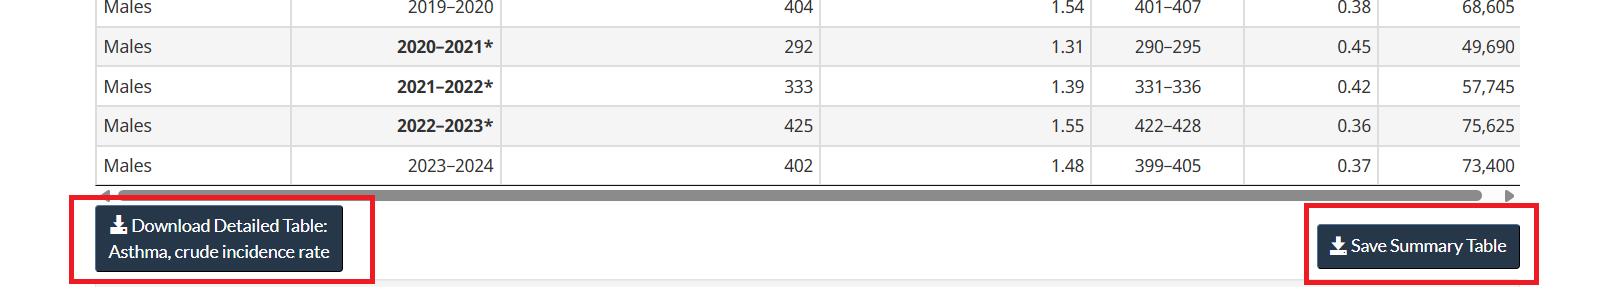
\includegraphics[width=0.9\linewidth,height=\textheight,keepaspectratio]{references/data-sources/../../assets/images/data9/ccdss9.png}
\end{center}

Once you open the CSV file in Excel or other software, you will find
that the data is not at the individual or person level. Instead, the
data are aggregated at the country and province/territory levels, and
summary measures are provided for both sexes and for years. For example,
see row 4. The \texttt{Geography} column says \emph{Canada} and the
\texttt{Rate\ (per\ 100,000)} column says \emph{919}. This is an example
of aggregate data.

\begin{center}
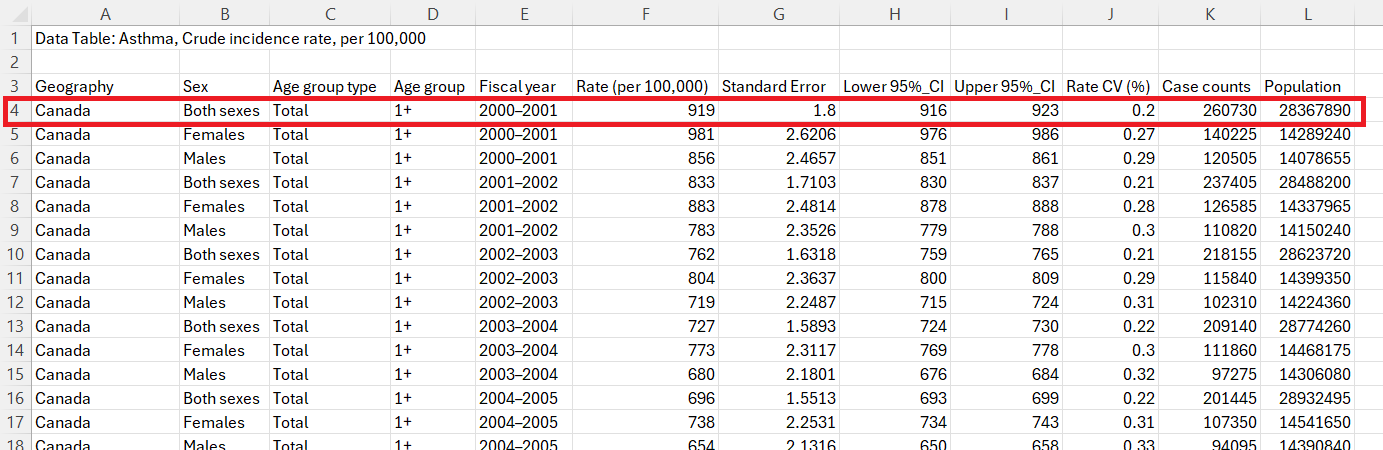
\includegraphics[width=0.9\linewidth,height=\textheight,keepaspectratio]{references/data-sources/../../assets/images/data9/ccdss10.png}
\end{center}

Because this data is not at the person-level, and the summary measures
are aggregated, you do not need a codebook to translate columns.
However, you cannot use this data to calculate the prevalence or
incidence of asthma in Canada because it is already aggregated. You can
only use this data to explore the trends over time, compare data across
provinces/territories, and view the distribution of cases by age group
and sex. The individual patients have already been erased to protect
their privacy.

\chapter*{Data Source: GHO}\label{data-source-gho}
\addcontentsline{toc}{chapter}{Data Source: GHO}

\markboth{Data Source: GHO}{Data Source: GHO}

The Global Health Observatory (GHO) is the World Health Organization's
(WHO) main health statistics repository. The GHO provides data on a wide
range of health topics, such as mortality, morbidity, risk factors,
health systems, and health equity. The GHO collects data from member
states, international organizations, and other sources to provide a
comprehensive picture of global health. The GHO is a valuable resource
for researchers, policymakers, and public health professionals who are
interested in understanding global health trends and disparities. The
GHO provides various ways to interact with its data, including
interactive maps and downloadable CSV files.

\begin{center}
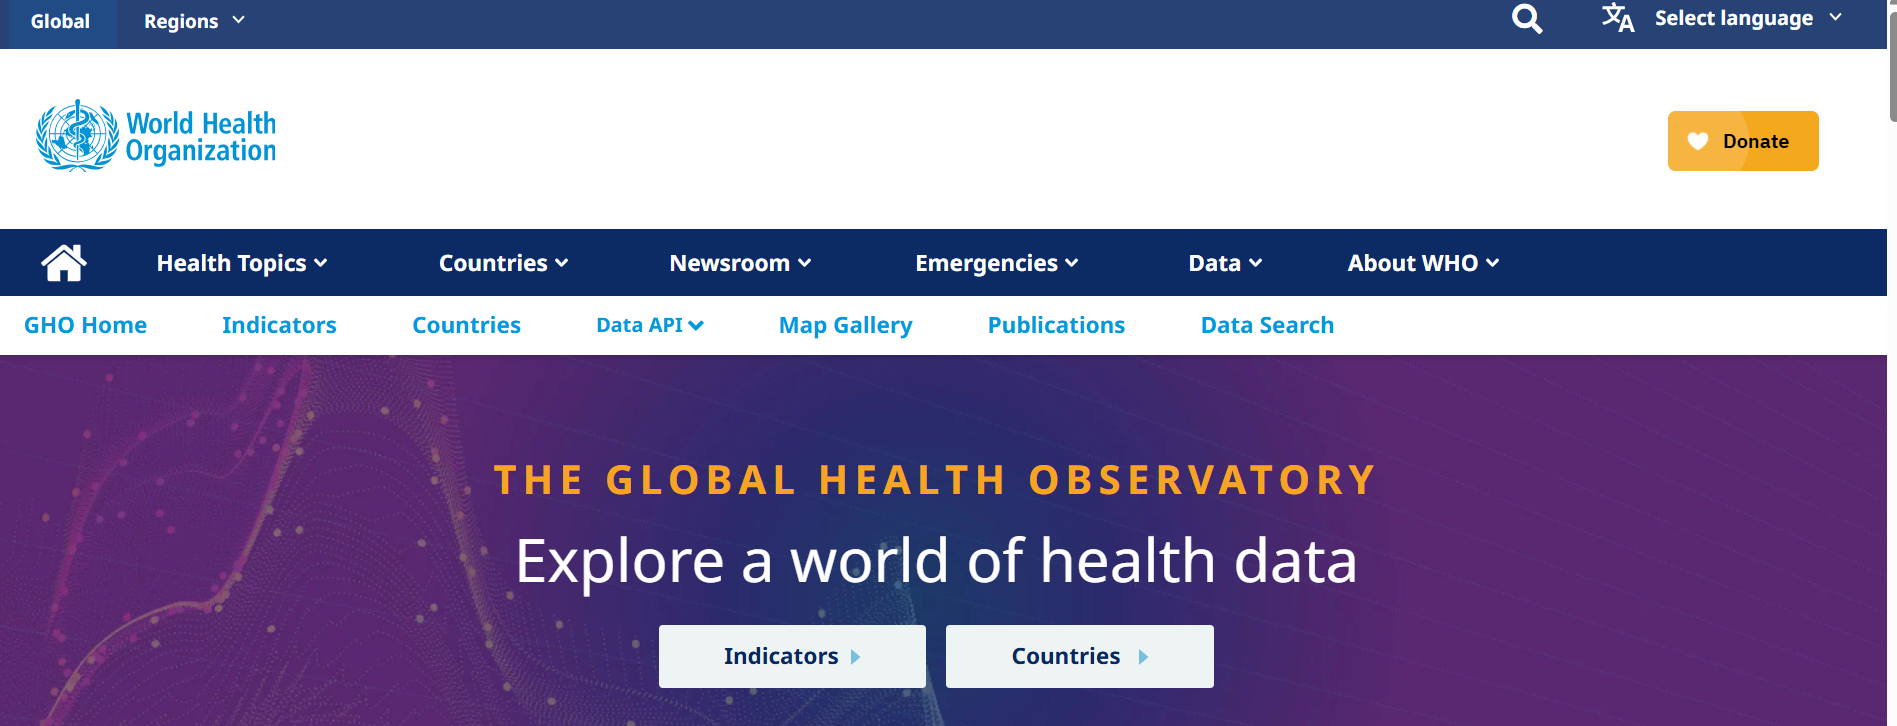
\includegraphics[width=0.9\linewidth,height=\textheight,keepaspectratio]{references/data-sources/../../assets/images/data10/gho1.png}
\end{center}

\marginnote{\begin{footnotesize}

\href{https://www.who.int/data/gho}{WHO Global Health Observatory}

\end{footnotesize}}

\subsection*{World Health Data}\label{world-health-data}
\addcontentsline{toc}{subsection}{World Health Data}

You can browse information by broader health indicators or by specific
countries.

\begin{center}

\includegraphics[width=0.9\linewidth,height=\textheight,keepaspectratio]{references/data-sources/../../assets/images/data10/gho2.png}
\end{center}

To explore the data by indicators, click on the \texttt{Indicators} tab.
You can find a list of indicators across categories such as
\texttt{Hepatitis}, \texttt{Nutrition}, \texttt{Mental\ health}, and so
on.

\begin{center}
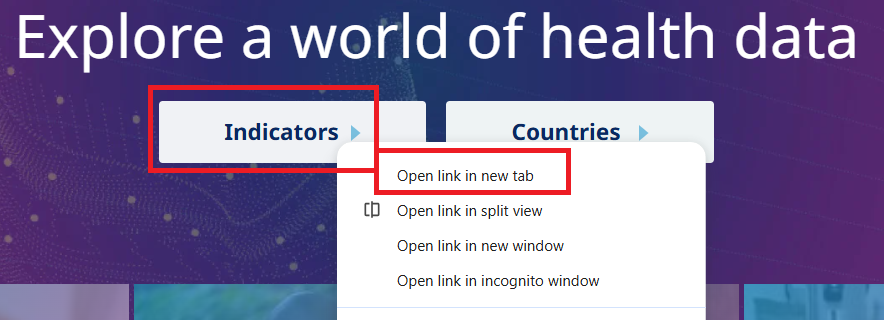
\includegraphics[width=0.9\linewidth,height=\textheight,keepaspectratio]{references/data-sources/../../assets/images/data10/gho3.png}
\end{center}

\begin{center}
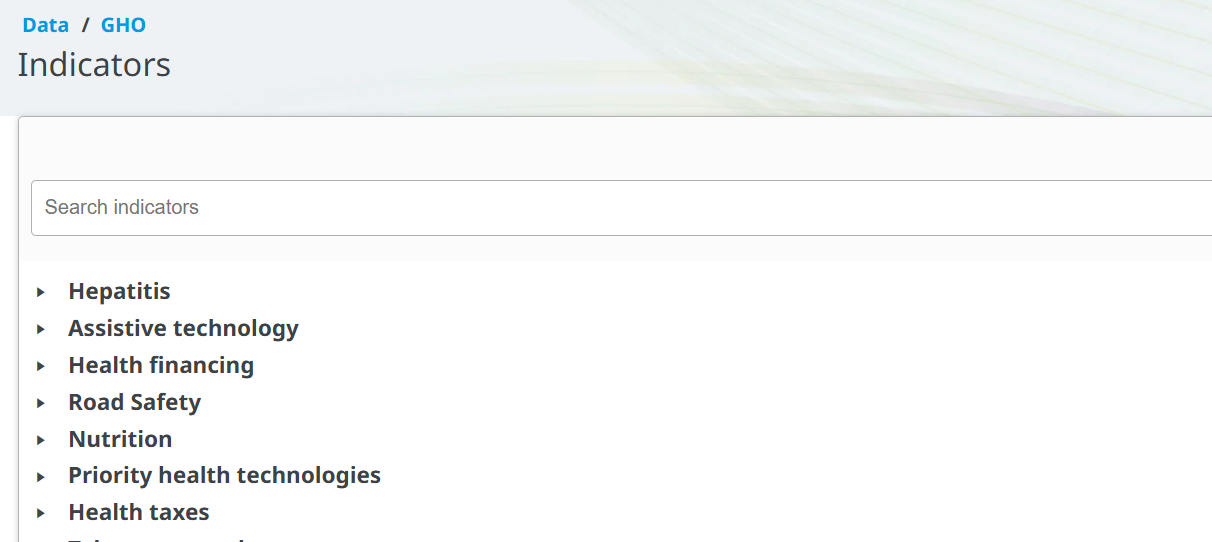
\includegraphics[width=0.9\linewidth,height=\textheight,keepaspectratio]{references/data-sources/../../assets/images/data10/gho4.png}
\end{center}

You can also use the search bar to search for specific indicators. For
example, if you search for \texttt{Life\ expectancy\ at\ birth}, you
will find a list of indicators related to life expectancy, such as
\texttt{Life\ expectancy\ at\ birth\ (years)}.

\begin{center}
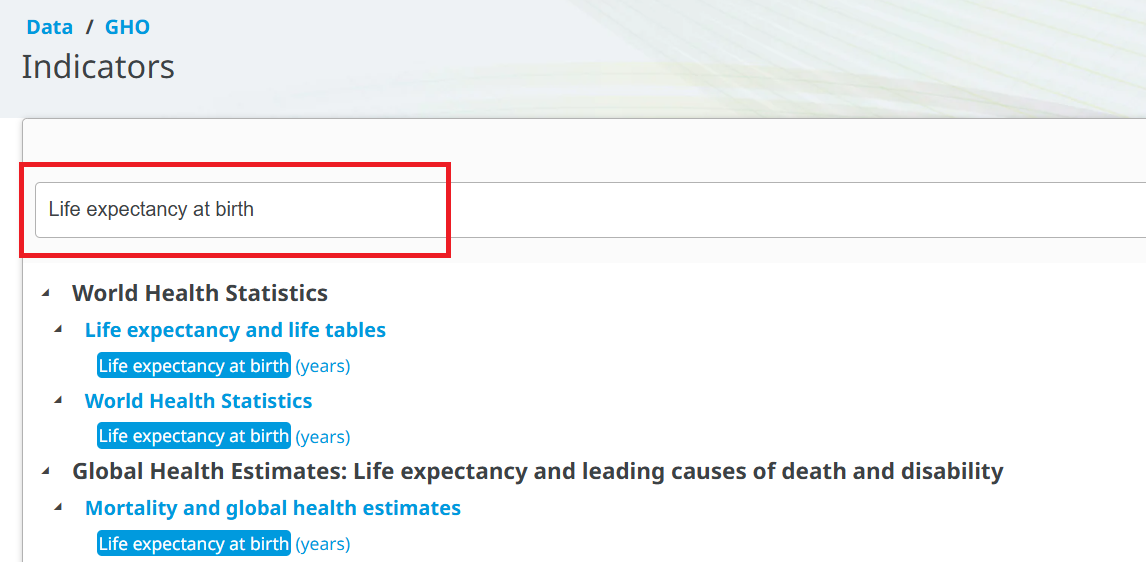
\includegraphics[width=0.9\linewidth,height=\textheight,keepaspectratio]{references/data-sources/../../assets/images/data10/gho5.png}
\end{center}

To explore the data by country, click on the \texttt{Countries} tab. You
can find a list of countries and regions. You can click the country name
to see the data for that country.

\begin{center}
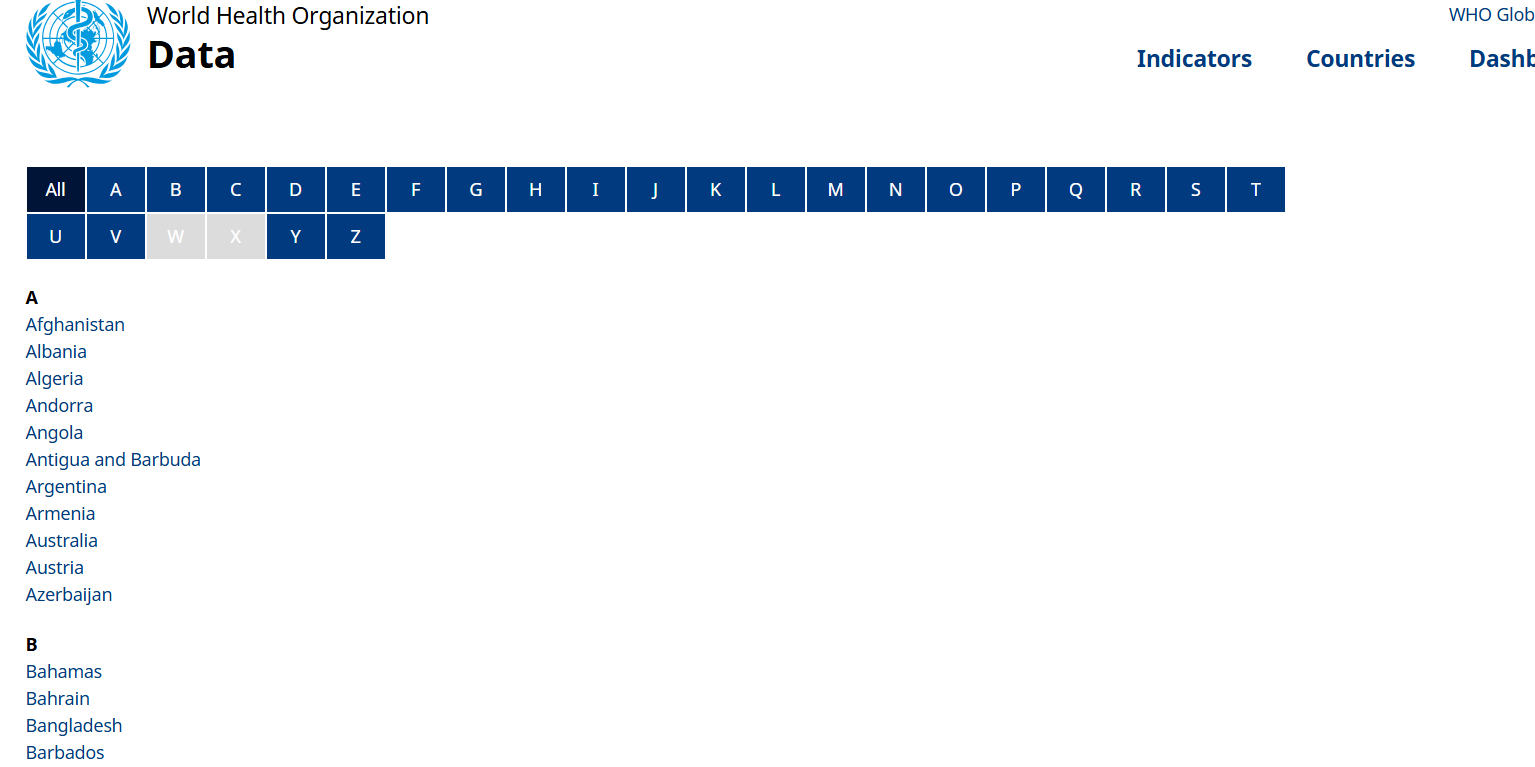
\includegraphics[width=0.9\linewidth,height=\textheight,keepaspectratio]{references/data-sources/../../assets/images/data10/gho6.png}
\end{center}

\begin{center}
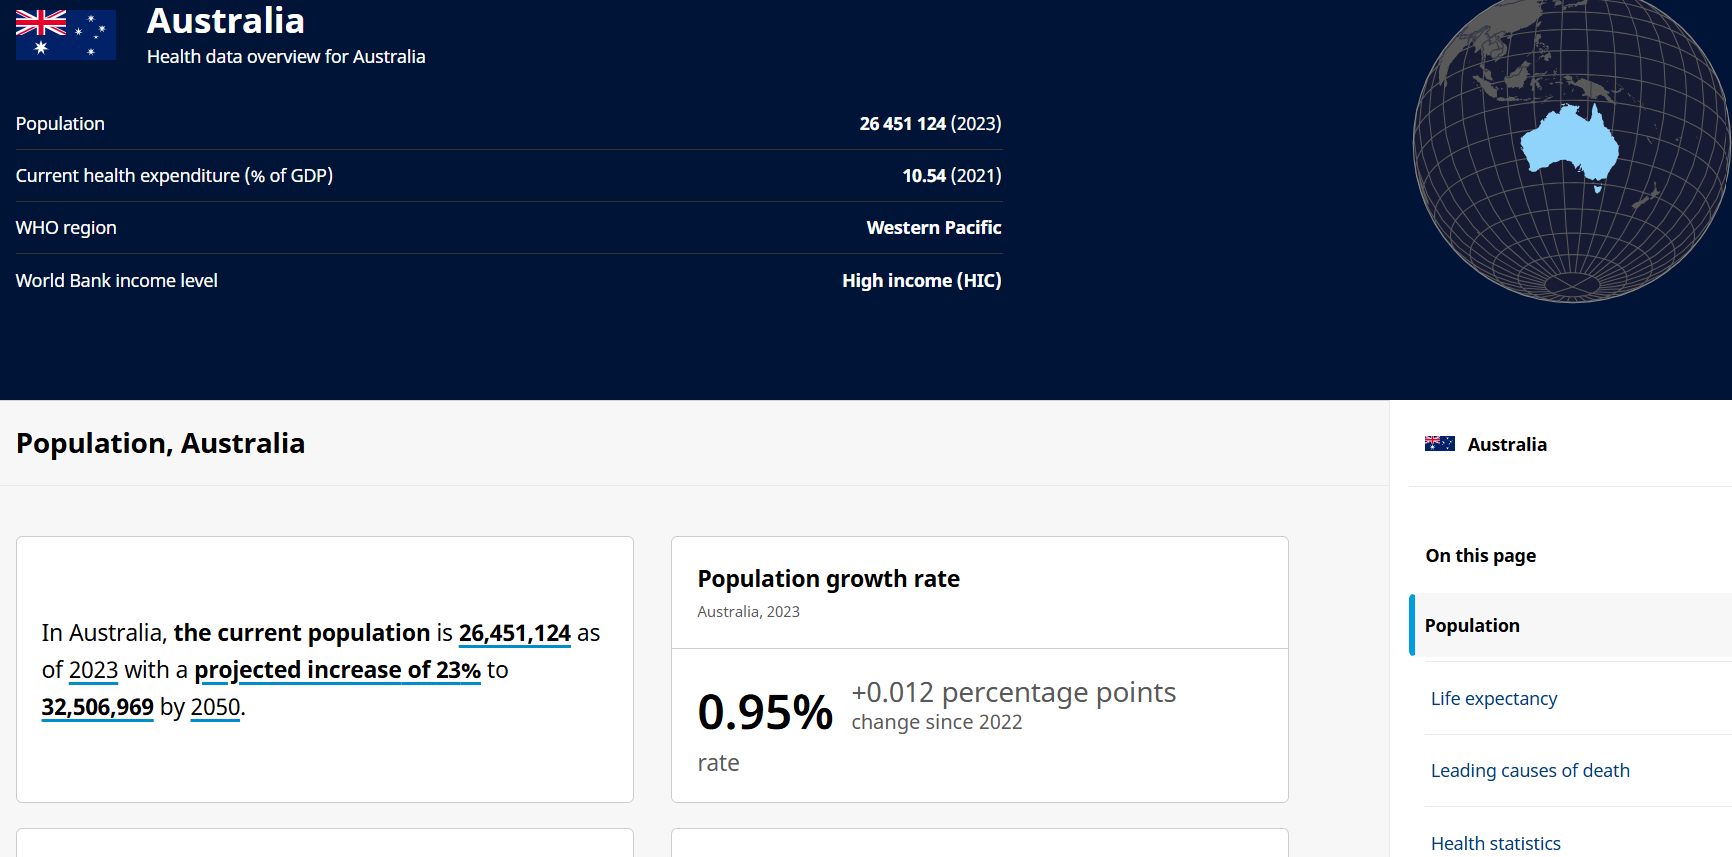
\includegraphics[width=0.9\linewidth,height=\textheight,keepaspectratio]{references/data-sources/../../assets/images/data10/gho7.png}
\end{center}

\subsection*{Data by indicator example}\label{data-by-indicator-example}
\addcontentsline{toc}{subsection}{Data by indicator example}

Let's click on the \texttt{Life\ expectancy\ at\ birth\ (years)}
indicator to see the details:

\begin{center}
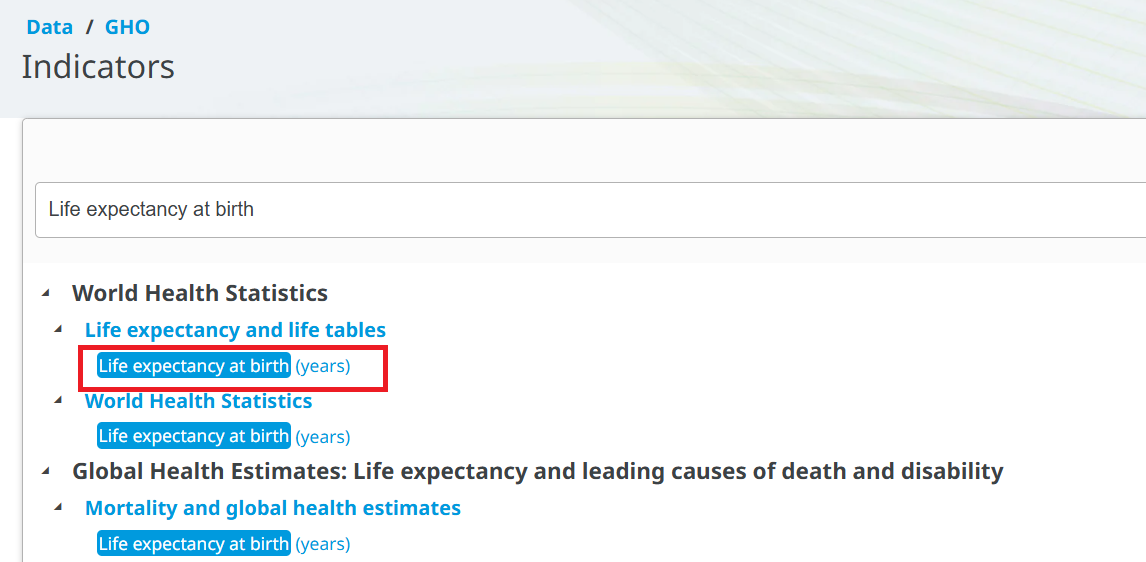
\includegraphics[width=0.9\linewidth,height=\textheight,keepaspectratio]{references/data-sources/../../assets/images/data10/gho8.png}
\end{center}

\marginnote{\begin{footnotesize}

\href{https://www.who.int/data/gho/data/indicators}{GHO Indicators}

\end{footnotesize}}

You can find different visualization options, such as charts and maps.
You can also download the chart and map to your computer.

\begin{center}
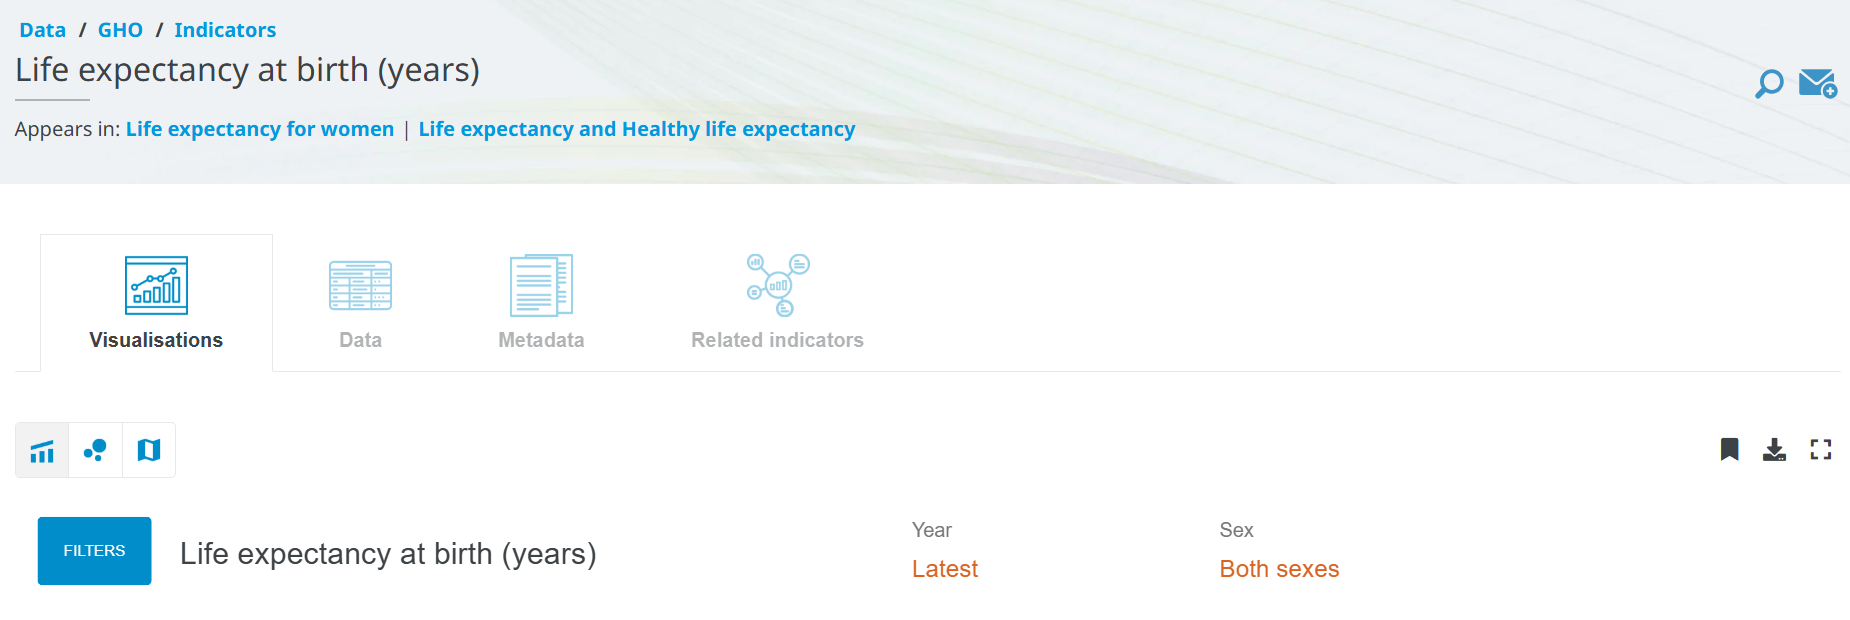
\includegraphics[width=1\linewidth,height=\textheight,keepaspectratio]{references/data-sources/../../assets/images/data10/gho9.png}
\end{center}

\begin{center}
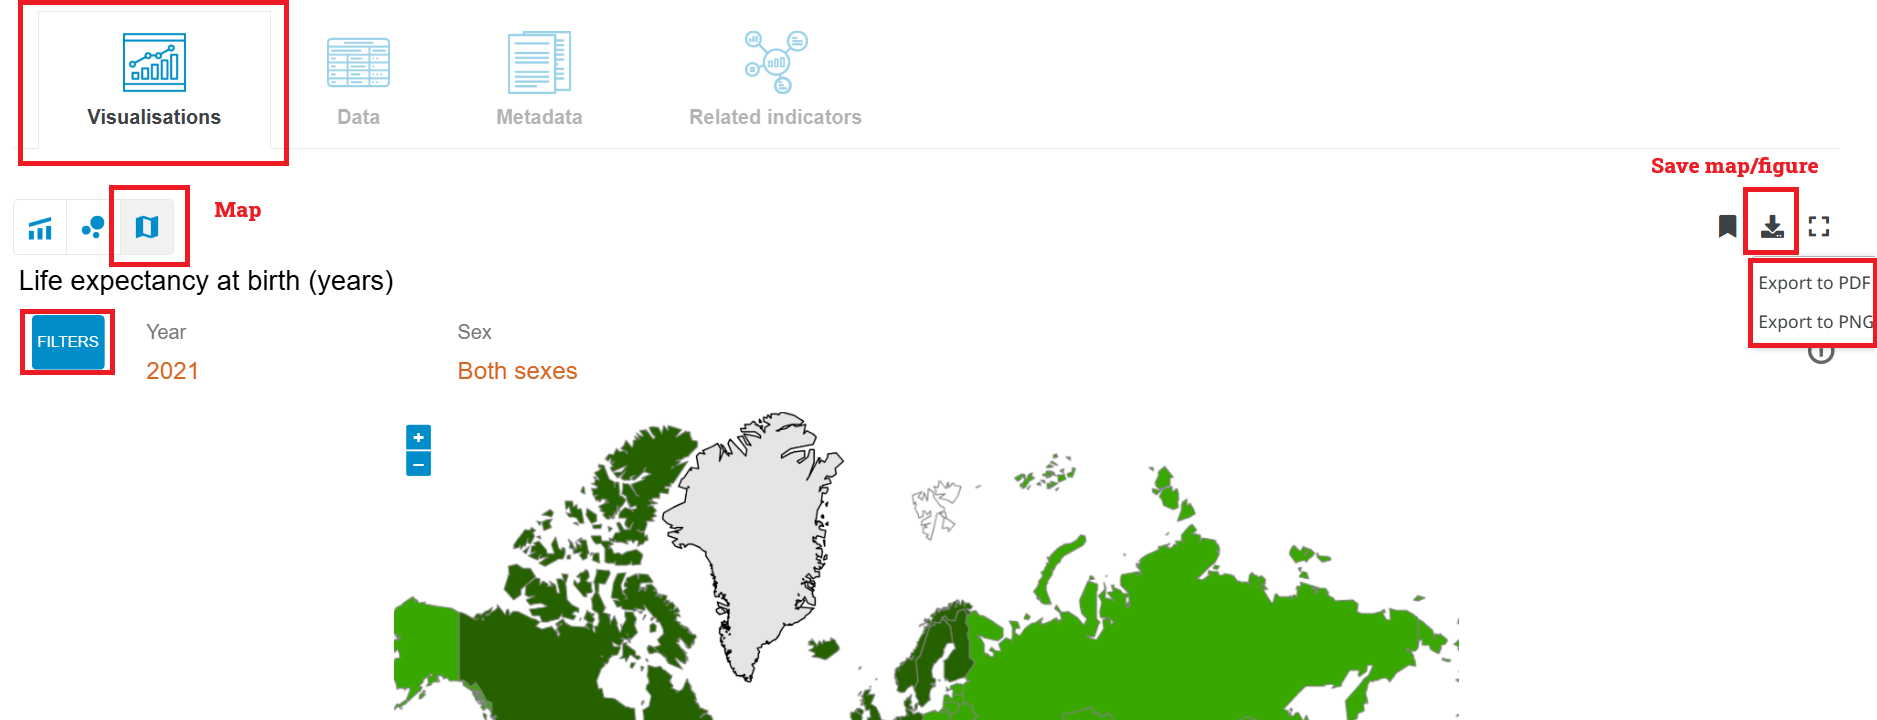
\includegraphics[width=1\linewidth,height=\textheight,keepaspectratio]{references/data-sources/../../assets/images/data10/gho10.png}
\end{center}

To see the data table, you can check the \texttt{Data} section. You can
also download the data in CSV format for further analysis. To do that,
you need to click on the \texttt{Download} button at the top right
corner of the data table.

\begin{center}
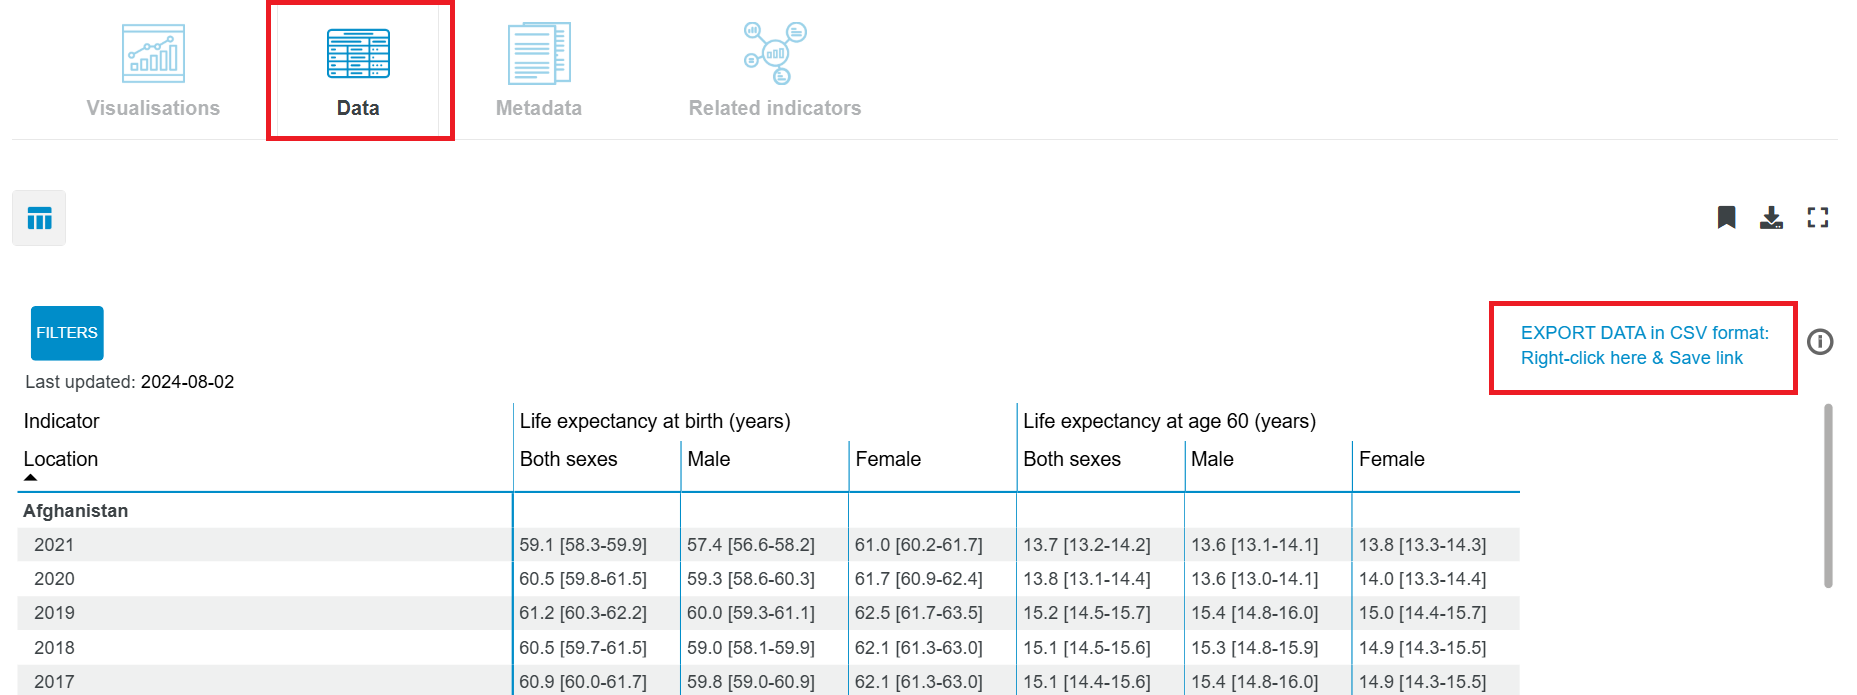
\includegraphics[width=1\linewidth,height=\textheight,keepaspectratio]{references/data-sources/../../assets/images/data10/gho11.png}
\end{center}

Similar to the \href{data9.html}{Canadian Chronic Disease Surveillance
System (CCDSS) database}, the life expectancy data is also at an
aggregated level, which means that the data is summarized at the country
level, and does not contain individual-level data:

\begin{center}
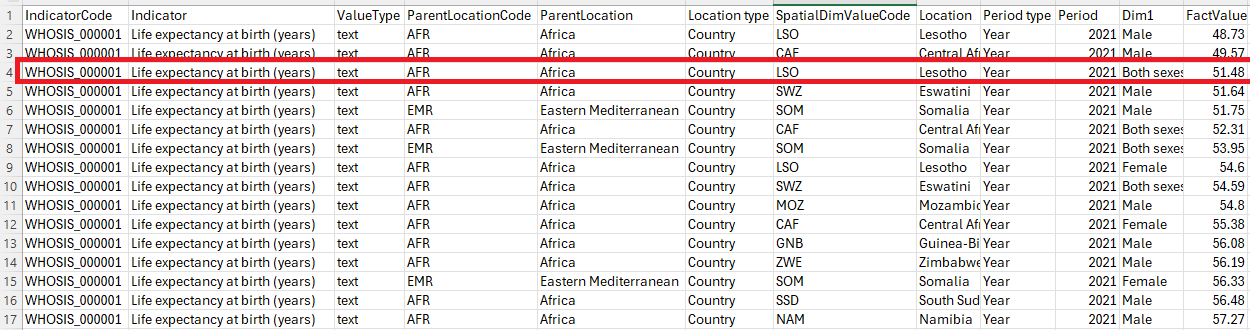
\includegraphics[width=1\linewidth,height=\textheight,keepaspectratio]{references/data-sources/../../assets/images/data10/gho12.png}
\end{center}

The data on the website, as well as the downloaded data in CSV format,
both provide the point estimate with 95\% confidence interval:

\begin{center}
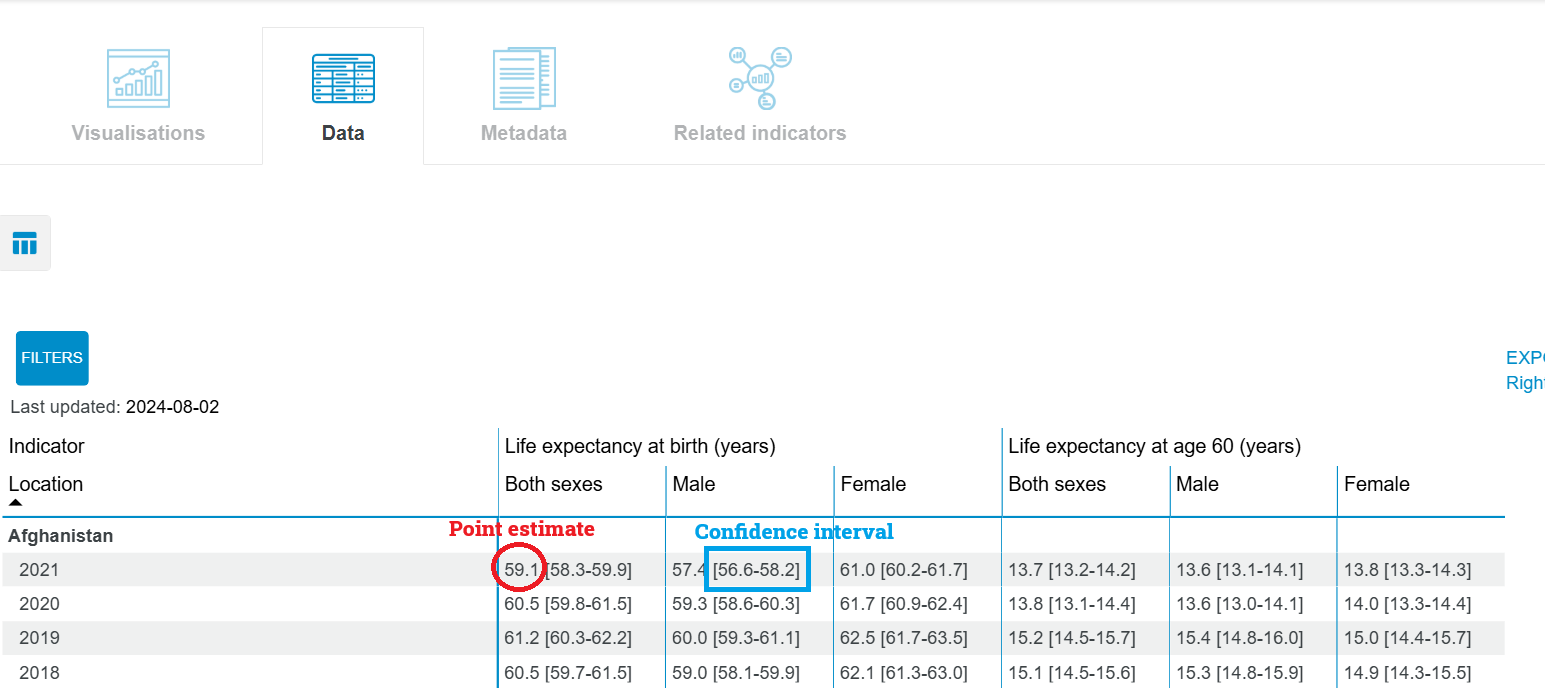
\includegraphics[width=1\linewidth,height=\textheight,keepaspectratio]{references/data-sources/../../assets/images/data10/gho13.png}
\end{center}

\subsection*{Data by country example}\label{data-by-country-example}
\addcontentsline{toc}{subsection}{Data by country example}

Let's click on \texttt{Canada} to explore the data for Canada.

\begin{center}
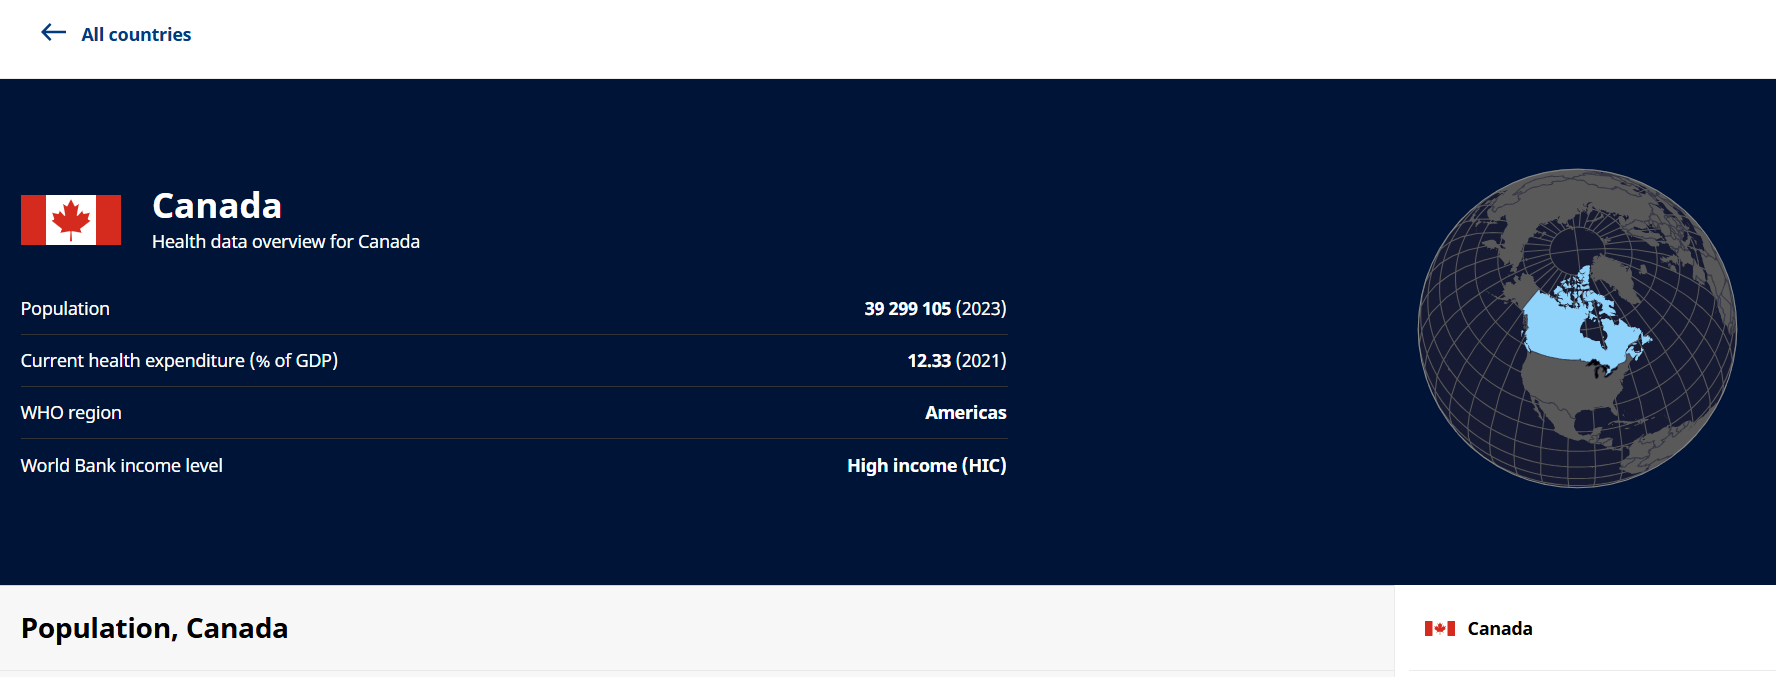
\includegraphics[width=0.9\linewidth,height=\textheight,keepaspectratio]{references/data-sources/../../assets/images/data10/gho14.png}
\end{center}

\marginnote{\begin{footnotesize}

\href{https://data.who.int/countries}{GHO Data by Country}

\end{footnotesize}}

You can explore different indicators for Canada. You can also download
all indicators as a ZIP file by clicking \texttt{Reference\ data}.

\begin{center}
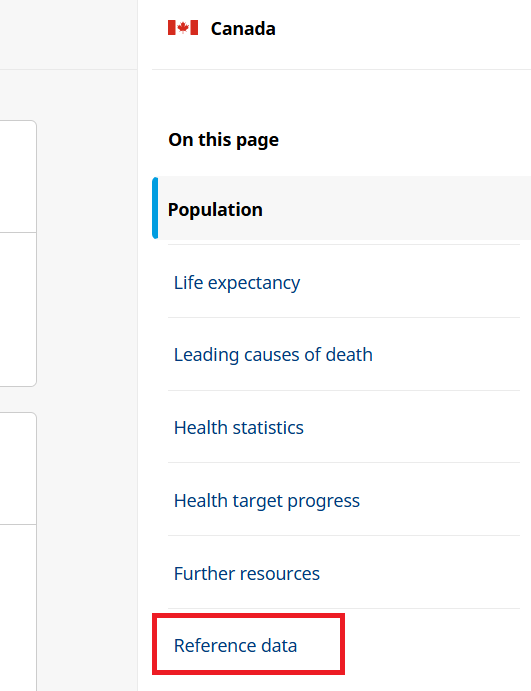
\includegraphics[width=0.75\linewidth,height=\textheight,keepaspectratio]{references/data-sources/../../assets/images/data10/gho15.png}
\end{center}

\begin{center}

\includegraphics[width=0.6\linewidth,height=\textheight,keepaspectratio]{references/data-sources/../../assets/images/data10/gho16.png}
\end{center}

Once you unzip the folder, you will find several folders. Each folder
contains a codelist, data, a data dictionary, along with a license and
terms of use for different indicators.

\begin{center}
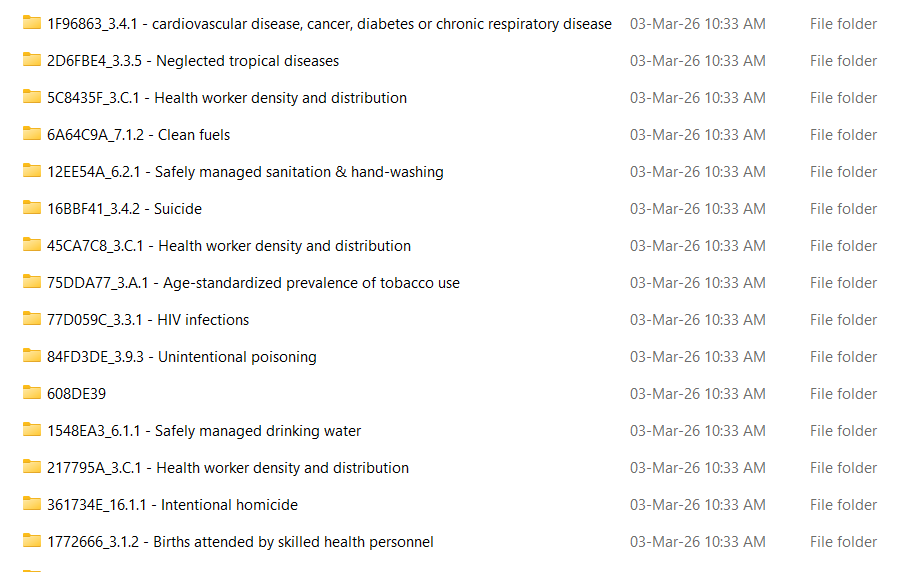
\includegraphics[width=0.9\linewidth,height=\textheight,keepaspectratio]{references/data-sources/../../assets/images/data10/gho17.png}
\end{center}

For example, the \texttt{77D059C\_3.3.1\ -\ HIV\ infections} folder
contains the following files:

\begin{center}
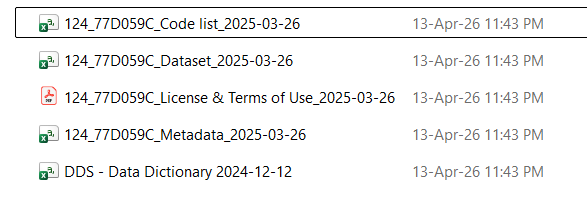
\includegraphics[width=0.9\linewidth,height=\textheight,keepaspectratio]{references/data-sources/../../assets/images/data10/gho18.png}
\end{center}

\subsection*{Metadata}\label{metadata}
\addcontentsline{toc}{subsection}{Metadata}

The GHO provides metadata for each indicator, providing important
context for understanding the data and its limitations. For example, the
metadata for the \texttt{Hepatitis\ -\ new\ infections} indicator
includes information on the definition of the indicator, the methods
used to calculate the indicator, data sources, and other relevant
information.

\marginnote{\begin{footnotesize}

\href{https://www.who.int/data/gho/indicator-metadata-registry}{Indicator
Metadata Registry List}

\end{footnotesize}}

\begin{center}
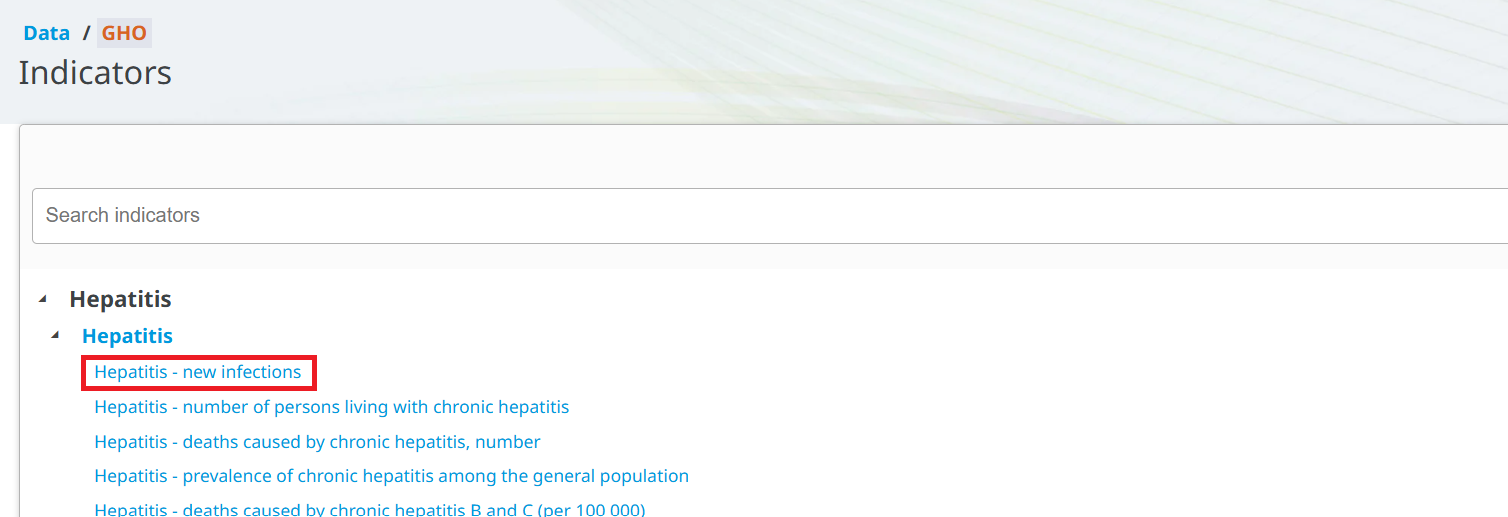
\includegraphics[width=1\linewidth,height=\textheight,keepaspectratio]{references/data-sources/../../assets/images/data10/gho19.png}
\end{center}

\begin{center}
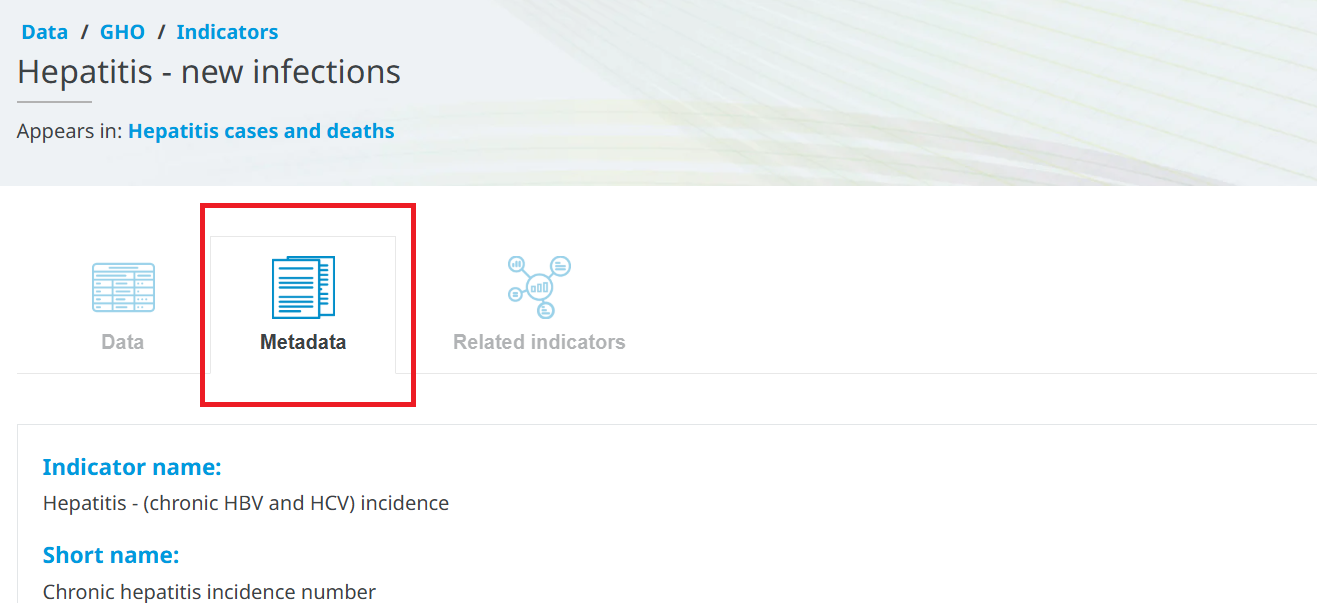
\includegraphics[width=1\linewidth,height=\textheight,keepaspectratio]{references/data-sources/../../assets/images/data10/gho20.png}
\end{center}

\chapter*{Data Source: Open Portal}\label{data-source-open-portal}
\addcontentsline{toc}{chapter}{Data Source: Open Portal}

\markboth{Data Source: Open Portal}{Data Source: Open Portal}

Open Government Portal Canada is a platform that provides access to
searching for a wide range of public data. Users can explore and
download data in different formats under the
\href{https://open.canada.ca/en/open-government-licence-canada}{Open
Government Licence - Canada}.

\begin{center}

\includegraphics[width=0.9\linewidth,height=\textheight,keepaspectratio]{references/data-sources/../../assets/images/data11/open1.png}
\end{center}

\marginnote{\begin{footnotesize}

\href{https://open.canada.ca/en}{Open Government Portal Canada}

\end{footnotesize}}

\subsection*{Search for Open Data}\label{search-for-open-data}
\addcontentsline{toc}{subsection}{Search for Open Data}

To search for open data, you can use the search bar on the Open
Government Portal Canada homepage. For example, if you are interested in
finding data on ``hospital locations'', you can enter that term in the
search bar and click the search icon. There are many filter options to
narrow your search results, such as format and organization.

\begin{center}
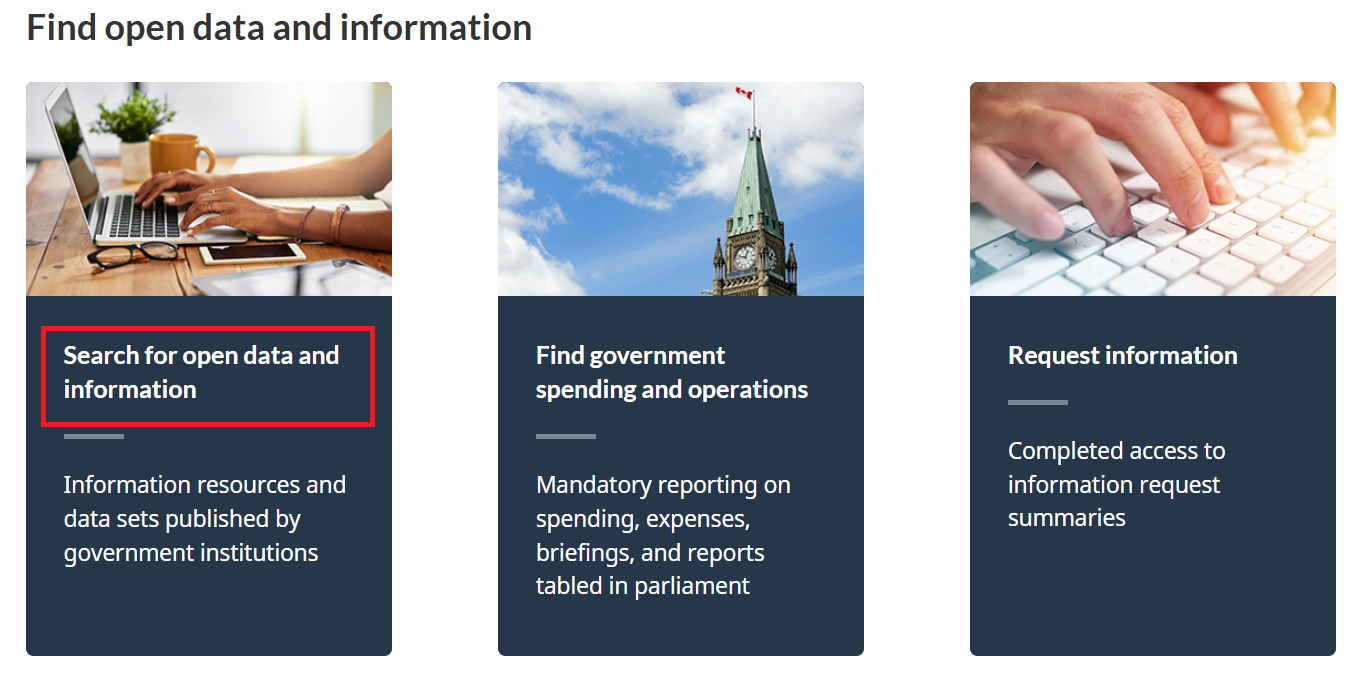
\includegraphics[width=0.9\linewidth,height=\textheight,keepaspectratio]{references/data-sources/../../assets/images/data11/open2.png}
\end{center}

\begin{center}
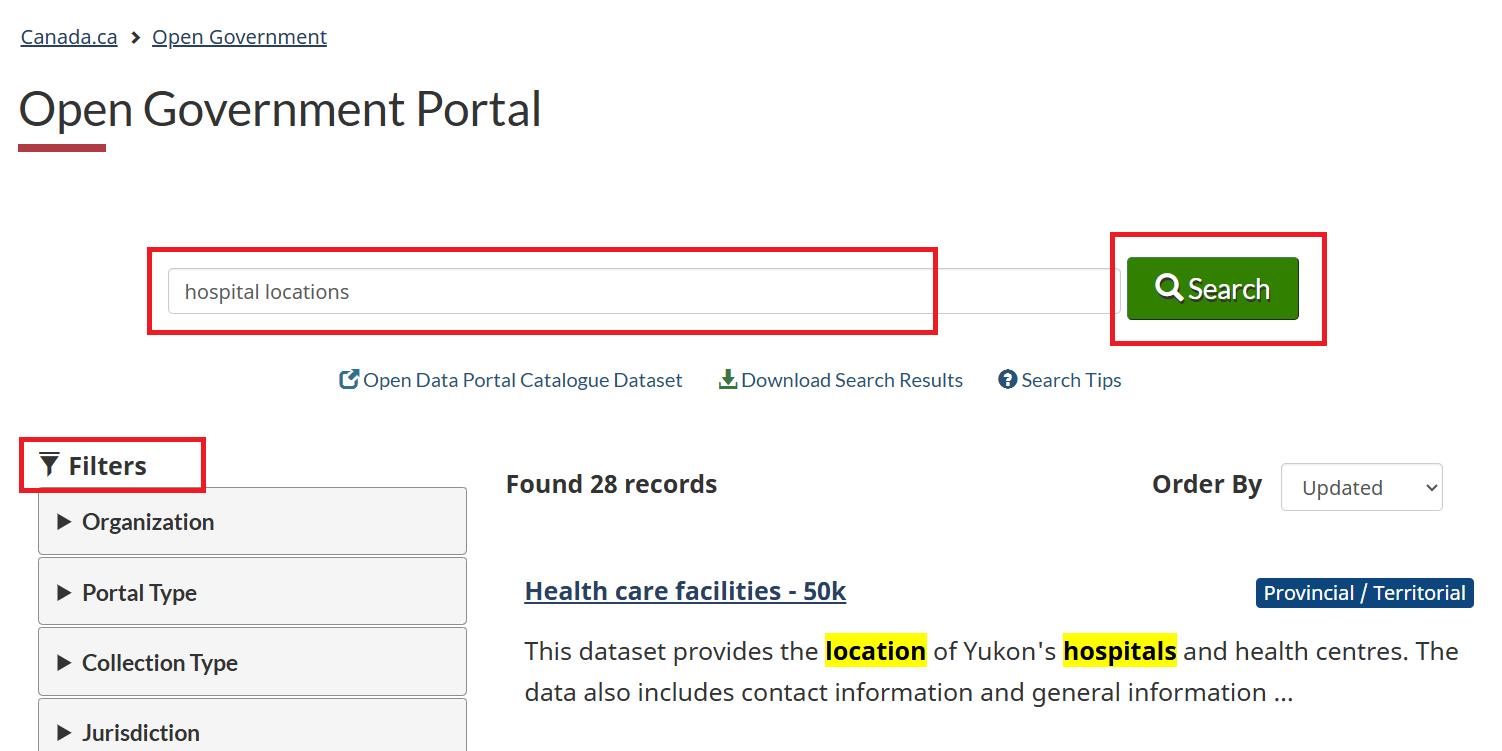
\includegraphics[width=0.9\linewidth,height=\textheight,keepaspectratio]{references/data-sources/../../assets/images/data11/open3.png}
\end{center}

To explore a specific dataset, click its title. This will take you to a
page with more information about the dataset, including its description,
format options, and download links. For example, if you click on the
``Health care facilities - 50k'' dataset, you will find detailed
information about the location of Yukon's hospitals and health centres.

\begin{center}
\includegraphics[width=0.9\linewidth,height=\textheight,keepaspectratio]{references/data-sources/../../assets/images/data11/open4.png}
\end{center}

\begin{center}
\includegraphics[width=0.9\linewidth,height=\textheight,keepaspectratio]{references/data-sources/../../assets/images/data11/open5.png}
\end{center}

Under the \texttt{Data\ and\ Resources} tab, you can find the available
formats for downloading the location of Yukon's hospitals and health
centres.

\begin{center}
\includegraphics[width=0.9\linewidth,height=\textheight,keepaspectratio]{references/data-sources/../../assets/images/data11/open6.png}
\end{center}

Similarly, say we are interested in ``opioid use'' and want to find open
data related to that topic. We can enter ``opioid use'' into the search
bar and filter by \texttt{Open\ data}:

\begin{center}
\includegraphics[width=0.9\linewidth,height=\textheight,keepaspectratio]{references/data-sources/../../assets/images/data11/open7.png}
\end{center}

To explore the data on opioid agonist treatment, we can click the
dataset title. This will take us to a page with more information about
the dataset, including its description, format options, and download
links.

\begin{center}
\includegraphics[width=0.9\linewidth,height=\textheight,keepaspectratio]{references/data-sources/../../assets/images/data11/open8.png}
\end{center}

\begin{center}
\includegraphics[width=0.9\linewidth,height=\textheight,keepaspectratio]{references/data-sources/../../assets/images/data11/open9.png}
\end{center}

\chapter*{Data Source: BC Data
Catalogue}\label{data-source-bc-data-catalogue}
\addcontentsline{toc}{chapter}{Data Source: BC Data Catalogue}

\markboth{Data Source: BC Data Catalogue}{Data Source: BC Data
Catalogue}

The British Columbia Data Catalogue is a central hub provided by the
Government of British Columbia (BC). Its primary purpose is to provide
public access to thousands of datasets managed by the provincial
government and its partners. Essentially, it is a digital library
designed to make government information transparent and usable for
citizens, researchers, and developers.

\begin{center}
\includegraphics[width=0.9\linewidth,height=\textheight,keepaspectratio]{references/data-sources/../../assets/images/data12/bc1.png}
\end{center}

\marginnote{\begin{footnotesize}

\href{https://catalogue.data.gov.bc.ca/}{British Columbia Data
Catalogue}

\end{footnotesize}}

\subsection*{Search for Data}\label{search-for-data}
\addcontentsline{toc}{subsection}{Search for Data}

To search for data, you can use the search bar on the BC Data Catalogue
homepage. For example, if you are interested in finding data on
``cancer'', you can enter that term in the search bar and click the
search icon.

\marginnote{\begin{footnotesize}

\href{https://catalogue.data.gov.bc.ca/datasets}{Search Data Catalogue}

\end{footnotesize}}

\begin{center}
\includegraphics[width=0.9\linewidth,height=\textheight,keepaspectratio]{references/data-sources/../../assets/images/data12/bc2.png}
\end{center}

\begin{center}
\includegraphics[width=1\linewidth,height=\textheight,keepaspectratio]{references/data-sources/../../assets/images/data12/bc3.png}
\end{center}

Similarly, say we are interested in ``COVID-19'' and want to find open
data related to that topic. We can enter ``covid'' into the search bar:

\begin{center}
\includegraphics[width=1\linewidth,height=\textheight,keepaspectratio]{references/data-sources/../../assets/images/data12/bc4.png}
\end{center}

You can filter your search by license, format, group, and so on:

\begin{center}
\includegraphics[width=1\linewidth,height=\textheight,keepaspectratio]{references/data-sources/../../assets/images/data12/bc5.png}
\end{center}

Let's explore the ``COVID-19 Case Details'' dataset. To do that, we can
click the dataset title. This will take us to a page with more
information about the dataset, including its description and related
links.

\begin{center}
\includegraphics[width=1\linewidth,height=\textheight,keepaspectratio]{references/data-sources/../../assets/images/data12/bc6.png}
\end{center}

You will find information on COVID-19 case details as well as a link to
download the data:

\begin{center}
\includegraphics[width=1\linewidth,height=\textheight,keepaspectratio]{references/data-sources/../../assets/images/data12/bc7.png}
\end{center}

To download the dataset, right-click on the \texttt{Access/Download}
link and select \texttt{Save\ link\ as...}. This will allow you to save
the dataset to your computer.

\begin{center}
\includegraphics[width=1\linewidth,height=\textheight,keepaspectratio]{references/data-sources/../../assets/images/data12/bc8.png}
\end{center}

\begin{center}
\includegraphics[width=0.9\linewidth,height=\textheight,keepaspectratio]{references/data-sources/../../assets/images/data12/bc9.png}
\end{center}

After downloading, you can open the data in Excel, Google Sheets, or any
statistical software. The data is structured in a tabular format, with
each row representing an individual case and each column representing
different variables.

\begin{center}
\includegraphics[width=0.9\linewidth,height=\textheight,keepaspectratio]{references/data-sources/../../assets/images/data12/bc10.png}
\end{center}

To learn more about BC Data Catalogue, click on the three bars on the
right side of the page:

\begin{center}
\includegraphics[width=0.8\linewidth,height=\textheight,keepaspectratio]{references/data-sources/../../assets/images/data12/bc11.png}
\end{center}

\part{Assistant Playbook}

\chapter*{Assistant Playbook}\label{assistant-playbook-1}
\addcontentsline{toc}{chapter}{Assistant Playbook}

\markboth{Assistant Playbook}{Assistant Playbook}

This playbook is for instructors, TAs, and AI assistants helping
maintain the HDSx course materials.

\section*{Operating Principles}\label{operating-principles}
\addcontentsline{toc}{section}{Operating Principles}

\markright{Operating Principles}

\begin{itemize}
\tightlist
\item
  Treat the syllabus as the source of truth for weeks, deliverables, and
  deadlines.
\item
  Keep student-facing content beginner-accessible and cloud-first.
\item
  Prefer reproducible Quarto, R, Python, and GitHub Codespaces workflows
  over local-machine assumptions.
\item
  Keep generated output separate from source content.
\item
  Add content where the normalized structure says it belongs: weeks,
  assignments, milestones, references, examples, or assets.
\end{itemize}

\section*{Editing Rules}\label{editing-rules}
\addcontentsline{toc}{section}{Editing Rules}

\markright{Editing Rules}

\begin{itemize}
\tightlist
\item
  Update \texttt{\_quarto.yml} whenever a page should appear in the
  book.
\item
  Keep paths relative and test them after moving files.
\item
  Use \texttt{assets/} for shared images and data that support teaching
  pages.
\item
  Use \texttt{examples/} for runnable code and sample datasets.
\item
  Do not bury assignment requirements only inside the syllabus; add a
  student-facing assignment or milestone brief.
\end{itemize}

\section*{Reproducibility
Expectations}\label{reproducibility-expectations}
\addcontentsline{toc}{section}{Reproducibility Expectations}

\markright{Reproducibility Expectations}

\begin{itemize}
\tightlist
\item
  Every activity should state expected inputs, outputs, and submission
  location.
\item
  Every code activity should run in a fresh GitHub Codespace.
\item
  Every dataset activity should record source, license, access date, and
  limitations.
\item
  Every AI-assisted activity should include an audit note: what AI
  helped with, what changed, and how the result was verified.
\end{itemize}

\section*{Review Cadence}\label{review-cadence}
\addcontentsline{toc}{section}{Review Cadence}

\markright{Review Cadence}

\begin{itemize}
\tightlist
\item
  Before term: verify links, screenshots, Codespace setup, dependencies,
  and all assignment briefs.
\item
  Weekly: update troubleshooting notes based on student issues.
\item
  Before each milestone: test the milestone instructions from a fresh
  repository.
\item
  After term: archive changes, refresh screenshots, and update the
  completion matrix.
\end{itemize}

\chapter*{Definition-of-Done
Checklists}\label{definition-of-done-checklists}
\addcontentsline{toc}{chapter}{Definition-of-Done Checklists}

\markboth{Definition-of-Done Checklists}{Definition-of-Done Checklists}

\section*{Course Page Done}\label{course-page-done}
\addcontentsline{toc}{section}{Course Page Done}

\markright{Course Page Done}

\begin{itemize}
\tightlist
\item
  The page appears in \texttt{\_quarto.yml} if it is student-facing.
\item
  The title matches the week or reference purpose.
\item
  Learning goals, activity steps, and expected outputs are clear.
\item
  Links and image paths render from the Quarto project root.
\item
  TODO blocks are either resolved or clearly scoped.
\end{itemize}

\section*{Assignment Done}\label{assignment-done}
\addcontentsline{toc}{section}{Assignment Done}

\markright{Assignment Done}

\begin{itemize}
\tightlist
\item
  The assignment has a student-facing brief.
\item
  Required files and submission location are explicit.
\item
  The work can be completed in GitHub Codespaces.
\item
  Packages, data, and outputs are documented.
\item
  The grading checklist matches the syllabus assessment logic.
\end{itemize}

\section*{Milestone Done}\label{milestone-done}
\addcontentsline{toc}{section}{Milestone Done}

\markright{Milestone Done}

\begin{itemize}
\tightlist
\item
  The milestone states the exact artifact students submit.
\item
  The milestone maps to the final portfolio.
\item
  The rubric includes reproducibility, auditability, data stewardship,
  and KT value.
\item
  Peer or TA review instructions are actionable.
\end{itemize}

\section*{Reproducibility Done}\label{reproducibility-done}
\addcontentsline{toc}{section}{Reproducibility Done}

\markright{Reproducibility Done}

\begin{itemize}
\tightlist
\item
  A fresh Codespace can render or run the project.
\item
  Paths are relative.
\item
  Dependencies are declared with \texttt{renv},
  \texttt{requirements.txt}, or a clearly documented equivalent.
\item
  No required data exists only on one person's local computer.
\item
  Randomness uses a seed when results depend on it.
\item
  The README explains how to reproduce the output.
\end{itemize}

\section*{AI Audit Done}\label{ai-audit-done}
\addcontentsline{toc}{section}{AI Audit Done}

\markright{AI Audit Done}

\begin{itemize}
\tightlist
\item
  The AI-use note says what tool was used and for what task.
\item
  Generated code was checked against real column names and expected
  outputs.
\item
  Generated summaries are grounded in actual results.
\item
  Security, privacy, and bias risks are considered.
\item
  The final text does not cite sources invented by AI.
\end{itemize}

\chapter{Syllabus-to-Content Coverage
Audit}\label{syllabus-to-content-coverage-audit}

Source of truth: \texttt{syllabus/SPPH-381H-Course-Outline-v4.qmd} and
\texttt{syllabus/syllabus-inventory-completion-matrix.md}.

Scope scanned: \texttt{\_quarto.yml}, \texttt{weeks/**.qmd},
\texttt{references/**.qmd}, \texttt{assignments/**}, and
\texttt{milestones/**}.

Decision rule: \textbf{Complete} requires both narrative coverage and a
runnable example, activity, exercise, or concrete student output.
\textbf{Needs Improvement} means content exists but is incomplete,
scaffold-only, TODO-heavy, or missing the exercise/example needed by the
syllabus. \textbf{Needs Review} means evidence is weak, ambiguous, or
outside the primary week/module.

\section{1) Executive Summary}\label{executive-summary}

\subsection{Status Counts}\label{status-counts}

\begin{itemize}
\tightlist
\item
  \textbf{Complete:} 3 topics
\item
  \textbf{Needs Improvement:} 11 topics
\item
  \textbf{Not Covered:} 0 topics
\item
  \textbf{Needs Review:} 1 topic
\end{itemize}

\subsection{Top 10 Highest-Priority
Gaps}\label{top-10-highest-priority-gaps}

\begin{enumerate}
\def\labelenumi{\arabic{enumi}.}
\tightlist
\item
  \textbf{Weeks 6-11 are scaffold-heavy.} Each has an overview, but most
  pages still contain \texttt{TODO\ Before\ Release} /
  \texttt{Content\ TODO} blocks rather than worked examples.
\item
  \textbf{Assignment briefs A1-A10 are stubs.} Every assignment README
  says \texttt{TODO:\ Build\ from\ assignments/assignment-template.qmd}.
\item
  \textbf{Milestone briefs M0-M5 and Final Portfolio are stubs and not
  in the Quarto TOC.} The milestone index is in the book, but the
  individual README briefs are orphaned.
\item
  \textbf{\texttt{renv} is promised in Week 3 but not taught with an
  activity.} Evidence is limited to assignment focus text and syllabus
  wording.
\item
  \textbf{Week 2 workflow mismatch: syllabus says fork a template,
  current content emphasizes GitHub Classroom.}
\item
  \textbf{Week 5 R deepening is weak.} Python/pandas coverage is
  substantial, but the syllabus promise of R mastery exercises on
  \texttt{dplyr} and functions is not clearly implemented in Week 5.
\item
  \textbf{Visualization lacks runnable ggplot2/plotly examples.} Week 6
  explicitly says to add worked examples and flawed/corrected AI plots.
\item
  \textbf{Dashboard pathway is undecided.} Week 8 says to decide between
  Quarto dashboard, Shiny, or static HTML/JS.
\item
  \textbf{Reporting/publishing lacks concrete citation and GitHub Pages
  workflow.} Week 10 lists these as TODOs.
\item
  \textbf{Presentation weeks lack rubric/timing/submission details.}
  Weeks 12-13 contain overviews but still call for presentation timing
  rules, peer feedback forms, and rubric links.
\end{enumerate}

\section{2) Coverage Matrix}\label{coverage-matrix}

\subsection{Week 0}\label{week-0}

\begin{itemize}
\tightlist
\item
  \textbf{Topic name (exact from syllabus):} Onboarding
\item
  \textbf{Status:} Needs Improvement
\item
  \textbf{Evidence:}

  \begin{itemize}
  \tightlist
  \item
    \texttt{syllabus/syllabus-inventory-completion-matrix.md} /
    \texttt{Extracted\ Schedule}: ``GitHub account, orientation video,
    pre-course survey.''
  \item
    \texttt{weeks/week00-onboarding/index.qmd} /
    \texttt{Required\ Student\ Tasks}: ``Create a GitHub account'';
    ``Watch the orientation video''; ``Complete the pre-course survey''.
  \item
    \texttt{weeks/week00-onboarding/index.qmd} / \texttt{Content\ TODO}:
    ``Add the actual Canvas orientation video link or placeholder.''
  \end{itemize}
\item
  \textbf{What's missing:}

  \begin{itemize}
  \tightlist
  \item
    Actual orientation video link or durable placeholder.
  \item
    Pre-course survey link or instructions.
  \item
    Clear confirmation/submission route.
  \end{itemize}
\item
  \textbf{Recommended next additions:}

  \begin{itemize}
  \tightlist
  \item
    Add a Canvas-link placeholder with release instructions.
  \item
    Add a short completion checklist students can self-verify.
  \item
    Add expected support/contact path for account setup failures.
  \end{itemize}
\end{itemize}

\subsection{Week 1}\label{week-1}

\begin{itemize}
\tightlist
\item
  \textbf{Topic name (exact from syllabus):} Health Data, KT \& Ethics
\item
  \textbf{Status:} Complete
\item
  \textbf{Evidence:}

  \begin{itemize}
  \tightlist
  \item
    \texttt{weeks/week01-health-data-ethics/index.qmd} /
    \texttt{Overview}: ``Knowledge Translation (KT)'' and ``ethical
    landscape of modern health data''.
  \item
    \texttt{weeks/week01-health-data-ethics/index.qmd} /
    \texttt{The\ Open\ Data\ Landscape}: ``Explore 2-3 portals''.
  \item
    \texttt{weeks/week01-health-data-ethics/index.qmd} /
    \texttt{The\ Data\ Intake\ Card}: fields for \texttt{dataset\_name},
    \texttt{portal\_url}, \texttt{licence\_terms}, and
    \texttt{stewardship\_notes}.
  \item
    \texttt{weeks/week01-health-data-ethics/activity-data-intake-card.qmd}
    / \texttt{Student\ Template}: copyable YAML-style template for the
    activity.
  \item
    \texttt{references/data-sources/nhis.qmd} /
    \texttt{Data\ Source:\ NHIS};
    \texttt{references/data-sources/nhanes.qmd} /
    \texttt{Data\ Source:\ NHANES}; plus other data-source reference
    pages.
  \end{itemize}
\item
  \textbf{What's missing:}

  \begin{itemize}
  \tightlist
  \item
    The activity page still has \texttt{TODO\ Before\ Release}.
  \item
    A short rubric for provenance/licensing/stewardship is requested but
    not present.
  \end{itemize}
\item
  \textbf{Recommended next additions:}

  \begin{itemize}
  \tightlist
  \item
    Add a student-facing rubric to
    \texttt{activity-data-intake-card.qmd}.
  \item
    Add one filled example Data Intake Card.
  \item
    Link the Week 1 page directly to relevant reference data-source
    pages.
  \end{itemize}
\end{itemize}

\subsection{Week 2}\label{week-2}

\begin{itemize}
\tightlist
\item
  \textbf{Topic name (exact from syllabus):} Modern Workflows
\item
  \textbf{Status:} Complete
\item
  \textbf{Evidence:}

  \begin{itemize}
  \tightlist
  \item
    \texttt{weeks/week02-modern-workflows/index.qmd} /
    \texttt{Getting\ Started:\ GitHub\ Account\ and\ Classroom}: account
    and repository setup steps.
  \item
    \texttt{weeks/week02-modern-workflows/index.qmd} /
    \texttt{Launching\ Your\ Codespace}: ``Create Codespace''.
  \item
    \texttt{weeks/week02-modern-workflows/index.qmd} /
    \texttt{Concepts:\ IDE,\ Notebook,\ Script}: compares IDE, script,
    notebook.
  \item
    \texttt{weeks/week02-modern-workflows/index.qmd} /
    \texttt{Concepts:\ Literate\ Programming}: ``Quarto documents mix
    Markdown text with code chunks.''
  \item
    \texttt{weeks/week02-modern-workflows/index.qmd} /
    \texttt{Tutorial:\ Stage,\ Commit,\ and\ Sync}: staged commit
    workflow.
  \item
    \texttt{weeks/week02-modern-workflows/index.qmd} /
    \texttt{Assignment\ 1:\ Your\ First\ Quarto\ Report}: concrete
    student task.
  \end{itemize}
\item
  \textbf{What's missing:}

  \begin{itemize}
  \tightlist
  \item
    Syllabus says ``Fork course template repo''; current content says
    GitHub Classroom/repository.
  \item
    Individual assignment folder is a stub even though the week page has
    a full assignment section.
  \end{itemize}
\item
  \textbf{Recommended next additions:}

  \begin{itemize}
  \tightlist
  \item
    Decide whether the official workflow is fork-based or GitHub
    Classroom, then align Week 2 and syllabus language.
  \item
    Move or mirror the Week 2 assignment instructions into
    \texttt{assignments/assignment01-workflows/README.md}.
  \end{itemize}
\end{itemize}

\subsection{Week 3}\label{week-3}

\begin{itemize}
\tightlist
\item
  \textbf{Topic name (exact from syllabus):} R with AI
\item
  \textbf{Status:} Needs Improvement
\item
  \textbf{Evidence:}

  \begin{itemize}
  \tightlist
  \item
    \texttt{weeks/week03-r-with-ai/index.qmd} /
    \texttt{Core\ Constructs}: variables, functions, and pipes.
  \item
    \texttt{weeks/week03-r-with-ai/index.qmd} /
    \texttt{Data\ Import\ and\ First\ Contact}:
    \texttt{read\_csv("data/patients.csv")}.
  \item
    \texttt{weeks/week03-r-with-ai/index.qmd} /
    \texttt{Data\ Transformation:\ The\ Five\ dplyr\ Verbs}:
    \texttt{filter}, \texttt{select}, \texttt{mutate},
    \texttt{summarise}, \texttt{group\_by}.
  \item
    \texttt{weeks/week03-r-with-ai/index.qmd} /
    \texttt{Writing\ a\ Simple\ Function}: reusable summary function.
  \item
    \texttt{weeks/week03-r-with-ai/index.qmd} /
    \texttt{Debugging:\ Reading\ the\ Red\ Text}: ``Fix It'' loop.
  \item
    \texttt{weeks/week03-r-with-ai/index.qmd} /
    \texttt{Assignment:\ The\ "Mad\ Libs"\ Report}: step-by-step
    workflow and deliverable.
  \item
    \texttt{assignments/assignment02-r-with-ai/README.md}: ``R basics,
    tidyverse transformations, custom functions, AI debugging, and
    \texttt{renv} awareness.''
  \end{itemize}
\item
  \textbf{What's missing:}

  \begin{itemize}
  \tightlist
  \item
    \texttt{renv} is promised in the syllabus as ``intro to renv for
    dependency management'' and ``initialize renv'', but no worked
    \texttt{renv::init()} / restore activity was found.
  \item
    Assignment 2 README is still a TODO stub.
  \end{itemize}
\item
  \textbf{Recommended next additions:}

  \begin{itemize}
  \tightlist
  \item
    Add a short \texttt{renv} tutorial/checkpoint to Week 3.
  \item
    Add \texttt{renv.lock} expectations and a recovery note.
  \item
    Expand \texttt{assignments/assignment02-r-with-ai/README.md} from
    the template.
  \end{itemize}
\end{itemize}

\subsection{Week 4}\label{week-4}

\begin{itemize}
\tightlist
\item
  \textbf{Topic name (exact from syllabus):} Git \& Collaboration
\item
  \textbf{Status:} Complete
\item
  \textbf{Evidence:}

  \begin{itemize}
  \tightlist
  \item
    \texttt{weeks/week04-git-collaboration/index.qmd} /
    \texttt{Save\ Game\ of\ Reproducible\ Science}: Git as provenance.
  \item
    \texttt{weeks/week04-git-collaboration/index.qmd} /
    \texttt{Repo\ Hygiene}: \texttt{.gitignore} and relative paths.
  \item
    \texttt{weeks/week04-git-collaboration/index.qmd} /
    \texttt{Branching:\ Safe\ Experimentation}: branch creation/merge
    tutorial.
  \item
    \texttt{weeks/week04-git-collaboration/index.qmd} /
    \texttt{Pull\ Requests:\ The\ Peer\ Review\ Gateway}: PR concept and
    tutorial.
  \item
    \texttt{weeks/week04-git-collaboration/index.qmd} /
    \texttt{Setting\ Up\ Your\ Group\ Repository}: term project group
    repository steps.
  \item
    \texttt{weeks/week04-git-collaboration/index.qmd} /
    \texttt{Practice\ Exercise:\ The\ Full\ Workflow\ Drill}: concrete
    exercise.
  \end{itemize}
\item
  \textbf{What's missing:}

  \begin{itemize}
  \tightlist
  \item
    M0 brief exists but is a TODO stub.
  \item
    Assignment 3 README exists but is a TODO stub.
  \end{itemize}
\item
  \textbf{Recommended next additions:}

  \begin{itemize}
  \tightlist
  \item
    Expand \texttt{milestones/m0-group-formation/README.md} with
    submission evidence.
  \item
    Expand \texttt{assignments/assignment03-git/README.md} with
    branch/PR screenshots or required proof.
  \end{itemize}
\end{itemize}

\subsection{Week 5}\label{week-5}

\begin{itemize}
\tightlist
\item
  \textbf{Topic name (exact from syllabus):} Polyglot Awareness \& R
  Deepening
\item
  \textbf{Status:} Needs Improvement
\item
  \textbf{Evidence:}

  \begin{itemize}
  \tightlist
  \item
    \texttt{weeks/week05-polyglot-r-deepening/index.qmd} /
    \texttt{Python\ vs\ R-\/-When\ and\ Why?}: ``R remains your primary
    analysis language.''
  \item
    \texttt{weeks/week05-polyglot-r-deepening/index.qmd} /
    \texttt{Loading\ and\ Viewing\ Data}:
    \texttt{pd.read\_csv("data/patients.csv")}.
  \item
    \texttt{weeks/week05-polyglot-r-deepening/index.qmd} /
    \texttt{Translation\ Traps}: zero-index, indentation,
    assignment/equality.
  \item
    \texttt{weeks/week05-polyglot-r-deepening/index.qmd} /
    \texttt{The\ AI\ Workflow:\ One\ Step,\ One\ Cell}: parity audit
    rules.
  \item
    \texttt{weeks/week05-polyglot-r-deepening/python13-translation-exercise.qmd}
    / \texttt{The\ Bilingual\ Translation\ Exercise}: practice exercise.
  \item
    \texttt{assignments/assignment04-polyglot/README.md}: ``reading
    Python/pandas, translating a small R task, and verifying parity.''
  \end{itemize}
\item
  \textbf{What's missing:}

  \begin{itemize}
  \tightlist
  \item
    Week 5 has strong Python coverage but weak explicit R-deepening
    exercises.
  \item
    Assignment 4 README is a TODO stub.
  \item
    Dependency documentation is covered for Python
    \texttt{requirements.txt}, but the syllabus framing of R deepening
    is not clearly tied to a student output.
  \end{itemize}
\item
  \textbf{Recommended next additions:}

  \begin{itemize}
  \tightlist
  \item
    Add one Week 5 exercise that repeats a task in R and Python and
    compares outputs.
  \item
    Add a specific R \texttt{dplyr}/function refinement task.
  \item
    Expand Assignment 4 into a concrete submission brief.
  \end{itemize}
\end{itemize}

\subsection{Week 6}\label{week-6}

\begin{itemize}
\tightlist
\item
  \textbf{Topic name (exact from syllabus):} Data Visualization
\item
  \textbf{Status:} Needs Improvement
\item
  \textbf{Evidence:}

  \begin{itemize}
  \tightlist
  \item
    \texttt{weeks/week06-visualization/index.qmd} / \texttt{Overview}:
    ``publication-quality visualizations'' and ``ggplot2 or plotly''.
  \item
    \texttt{weeks/week06-visualization/index.qmd} /
    \texttt{Content\ TODO}: ``Add a worked ggplot2 example''; ``Add one
    intentionally misleading AI-generated chart''.
  \item
    \texttt{weeks/week06-visualization/activity-ai-visual-audit.qmd} /
    \texttt{Goal}: evaluate ``correctness, clarity, bias, aggregation
    choices, and misleading design.''
  \item
    \texttt{assignments/assignment05-visualization/README.md}:
    ``original plot, revised plot, and audit note.''
  \end{itemize}
\item
  \textbf{What's missing:}

  \begin{itemize}
  \tightlist
  \item
    Worked ggplot2 example.
  \item
    Plotly or interactive extension.
  \item
    Flawed AI chart plus corrected version.
  \item
    Concrete starter data and prompt.
  \end{itemize}
\item
  \textbf{Recommended next additions:}

  \begin{itemize}
  \tightlist
  \item
    Add a runnable ggplot2 tutorial using shared data.
  \item
    Add one intentionally flawed chart and student audit questions.
  \item
    Add a small plotly extension as optional enrichment.
  \end{itemize}
\end{itemize}

\subsection{Week 7}\label{week-7}

\begin{itemize}
\tightlist
\item
  \textbf{Topic name (exact from syllabus):} EDA, Table 1 \& AI Auditing
\item
  \textbf{Status:} Needs Improvement
\item
  \textbf{Evidence:}

  \begin{itemize}
  \tightlist
  \item
    \texttt{weeks/week07-eda-ai-audit/index.qmd} / \texttt{Overview}:
    EDA and ``standard Table 1''.
  \item
    \texttt{weeks/week07-eda-ai-audit/index.qmd} /
    \texttt{Content\ TODO}: ``Build a worked EDA''; ``Add Table 1
    expectations''; ``Add a planted-error AI audit exercise.''
  \item
    \texttt{weeks/week07-eda-ai-audit/activity-table1-audit.qmd} /
    \texttt{Goal}: ``create a descriptive summary and audit AI-generated
    code''.
  \item
    \texttt{assignments/assignment06-eda-ai-audit/README.md}: ``EDA,
    Table 1 or equivalent descriptive summary, planted-error audit, and
    provenance notes.''
  \end{itemize}
\item
  \textbf{What's missing:}

  \begin{itemize}
  \tightlist
  \item
    Worked EDA with data path.
  \item
    Table 1 variables and example output.
  \item
    Planted-error code/summary/visualization.
  \item
    Instructor key outside student page.
  \end{itemize}
\item
  \textbf{Recommended next additions:}

  \begin{itemize}
  \tightlist
  \item
    Build around \texttt{examples/data/} or a week-local starter
    dataset.
  \item
    Add a runnable Table 1 example.
  \item
    Add AI audit prompts and expected fixes.
  \end{itemize}
\end{itemize}

\subsection{Week 8}\label{week-8}

\begin{itemize}
\tightlist
\item
  \textbf{Topic name (exact from syllabus):} Dashboard Prototypes for KT
\item
  \textbf{Status:} Needs Improvement
\item
  \textbf{Evidence:}

  \begin{itemize}
  \tightlist
  \item
    \texttt{weeks/week08-dashboard-kt/index.qmd} / \texttt{Overview}:
    Shiny apps, dashboards, and KT.
  \item
    \texttt{weeks/week08-dashboard-kt/index.qmd} /
    \texttt{Content\ TODO}: ``Decide the required core pathway''; ``Add
    a minimal dashboard starter''.
  \item
    \texttt{weeks/week08-dashboard-kt/starter-dashboard.qmd} /
    \texttt{Required\ Elements}: audience-specific question, control,
    visualization, interpretation, limitation.
  \item
    \texttt{assignments/assignment07-dashboard/README.md}: ``minimal
    dashboard-style KT product from EDA outputs.''
  \end{itemize}
\item
  \textbf{What's missing:}

  \begin{itemize}
  \tightlist
  \item
    Actual dashboard code.
  \item
    Required pathway decision: Quarto dashboard, Shiny, or static
    HTML/JS.
  \item
    Codespaces testing instructions.
  \item
    Privacy-safe publishing guidance.
  \end{itemize}
\item
  \textbf{Recommended next additions:}

  \begin{itemize}
  \tightlist
  \item
    Add a minimal Quarto dashboard starter that renders.
  \item
    Add a fallback static version.
  \item
    State which pathway is required and which are optional.
  \end{itemize}
\end{itemize}

\subsection{Week 9}\label{week-9}

\begin{itemize}
\tightlist
\item
  \textbf{Topic name (exact from syllabus):} Communication of Scientific
  Findings
\item
  \textbf{Status:} Needs Improvement
\item
  \textbf{Evidence:}

  \begin{itemize}
  \tightlist
  \item
    \texttt{weeks/week09-science-communication/index.qmd} /
    \texttt{Overview}: ``Audience-Specific KT'', plain language, slide
    decks, peer review.
  \item
    \texttt{weeks/week09-science-communication/index.qmd} /
    \texttt{Content\ TODO}: ``Add a revealjs starter deck''; ``Add a
    plain-language summary exercise.''
  \item
    \texttt{weeks/week09-science-communication/revealjs-peer-feedback.qmd}
    / \texttt{Peer\ Feedback\ Prompts}: main message, evidence,
    overclaiming, reproducibility/audience fit.
  \item
    \texttt{assignments/assignment08-communication/README.md}:
    ``revealjs slides, plain-language summary, citations, and peer
    feedback.''
  \end{itemize}
\item
  \textbf{What's missing:}

  \begin{itemize}
  \tightlist
  \item
    Minimal \texttt{format:\ revealjs} example.
  \item
    Three-slide starter structure.
  \item
    Plain-language summary exercise.
  \item
    Citation and accessibility expectations.
  \end{itemize}
\item
  \textbf{Recommended next additions:}

  \begin{itemize}
  \tightlist
  \item
    Add a renderable revealjs starter.
  \item
    Add a before/after plain-language translation activity.
  \item
    Convert peer prompts into a reusable feedback form.
  \end{itemize}
\end{itemize}

\subsection{Week 10}\label{week-10}

\begin{itemize}
\tightlist
\item
  \textbf{Topic name (exact from syllabus):} Writing \& Publishing
  Reports
\item
  \textbf{Status:} Needs Improvement
\item
  \textbf{Evidence:}

  \begin{itemize}
  \tightlist
  \item
    \texttt{weeks/week10-reporting-publishing/index.qmd} /
    \texttt{Overview}: dynamic report and publishing workflows.
  \item
    \texttt{weeks/week10-reporting-publishing/index.qmd} /
    \texttt{Content\ TODO}: report skeleton, citation examples, GitHub
    Pages setup, grounding audit.
  \item
    \texttt{weeks/week10-reporting-publishing/report-template.qmd} /
    \texttt{Suggested\ Sections}: question, data, methods, results,
    limitations, plain-language summary, AI-use note.
  \item
    \texttt{assignments/assignment09-reporting/README.md}: ``Quarto
    report, citations, GitHub Pages or private equivalent, and grounding
    audit.''
  \end{itemize}
\item
  \textbf{What's missing:}

  \begin{itemize}
  \tightlist
  \item
    Copyable report starter with real YAML.
  \item
    Bibliography setup and citation example.
  \item
    GitHub Pages setup or private submission alternative.
  \item
    Interactive element example.
  \end{itemize}
\item
  \textbf{Recommended next additions:}

  \begin{itemize}
  \tightlist
  \item
    Add a minimal report template that renders with
    \texttt{references.bib}.
  \item
    Add a GitHub Pages checklist with screenshots or text-only steps.
  \item
    Add citation grounding audit prompts.
  \end{itemize}
\end{itemize}

\subsection{Week 11}\label{week-11}

\begin{itemize}
\tightlist
\item
  \textbf{Topic name (exact from syllabus):} Portfolio Surgery \&
  Optional Advanced Deployment
\item
  \textbf{Status:} Needs Improvement
\item
  \textbf{Evidence:}

  \begin{itemize}
  \tightlist
  \item
    \texttt{weeks/week11-portfolio-surgery/index.qmd} /
    \texttt{Overview}: dependency management, auditability, and peer
    review.
  \item
    \texttt{weeks/week11-portfolio-surgery/index.qmd} /
    \texttt{Content\ TODO}: fresh Codespace test, broken-project
    exercise, Assignment 10, Milestone 4, final checklist.
  \item
    \texttt{weeks/week11-portfolio-surgery/reproducibility-test.qmd} /
    \texttt{Failure\ Log\ Template}: checks for repository, packages,
    report, dashboard, README.
  \item
    \texttt{assignments/assignment10-portfolio-surgery/README.md}:
    ``fresh Codespace test, dependency/path repair, README clarity''.
  \item
    \texttt{milestones/m4-peer-review/README.md}: peer review covering
    clarity, reproducibility, auditability, KT value.
  \end{itemize}
\item
  \textbf{What's missing:}

  \begin{itemize}
  \tightlist
  \item
    Step-by-step fresh Codespace protocol.
  \item
    Broken-project debugging exercise.
  \item
    Final portfolio readiness checklist.
  \item
    Optional Python-flavoured pathway from syllabus is not clearly
    present here.
  \end{itemize}
\item
  \textbf{Recommended next additions:}

  \begin{itemize}
  \tightlist
  \item
    Expand \texttt{reproducibility-test.qmd} into a runbook.
  \item
    Add a sample failure log with fixes.
  \item
    Add a final portfolio checklist linked from Week 11 and final
    portfolio README.
  \end{itemize}
\end{itemize}

\subsection{Week 12}\label{week-12}

\begin{itemize}
\tightlist
\item
  \textbf{Topic name (exact from syllabus):} Term Project Presentations,
  Part 1
\item
  \textbf{Status:} Needs Improvement
\item
  \textbf{Evidence:}

  \begin{itemize}
  \tightlist
  \item
    \texttt{weeks/week12-presentations/index.qmd} / \texttt{Overview}:
    first presentation block and peer review.
  \item
    \texttt{weeks/week12-presentations/index.qmd} /
    \texttt{Content\ TODO}: timing rules, slide submission, peer
    feedback form, rubric.
  \item
    \texttt{milestones/m5-presentation/README.md}: ``presentation
    slides, live Q\&A, and peer review feedback.''
  \end{itemize}
\item
  \textbf{What's missing:}

  \begin{itemize}
  \tightlist
  \item
    Presentation timing rules.
  \item
    Slide submission instructions.
  \item
    Peer feedback form.
  \item
    Presentation rubric.
  \end{itemize}
\item
  \textbf{Recommended next additions:}

  \begin{itemize}
  \tightlist
  \item
    Add a M5 rubric and link it from Week 12.
  \item
    Add a slide checklist and submission timing.
  \item
    Add a simple peer feedback form.
  \end{itemize}
\end{itemize}

\subsection{Week 13}\label{week-13}

\begin{itemize}
\tightlist
\item
  \textbf{Topic name (exact from syllabus):} Term Project Presentations,
  Part 2
\item
  \textbf{Status:} Needs Improvement
\item
  \textbf{Evidence:}

  \begin{itemize}
  \tightlist
  \item
    \texttt{weeks/week13-presentations/index.qmd} / \texttt{Overview}:
    completes M5 and feedback before final portfolio.
  \item
    \texttt{weeks/week13-presentations/index.qmd} /
    \texttt{Content\ TODO}: group schedule, final reminders, closing
    reflection prompt.
  \item
    \texttt{milestones/m5-presentation/README.md}: ``slides render
    before class and claims are grounded''.
  \end{itemize}
\item
  \textbf{What's missing:}

  \begin{itemize}
  \tightlist
  \item
    Group schedule or placeholder.
  \item
    Final portfolio reminders.
  \item
    Closing reflection prompt.
  \end{itemize}
\item
  \textbf{Recommended next additions:}

  \begin{itemize}
  \tightlist
  \item
    Add a repeatable Part 2 logistics block.
  \item
    Link to final portfolio checklist.
  \item
    Add a reflection prompt on reproducibility and KT.
  \end{itemize}
\end{itemize}

\subsection{Final}\label{final}

\begin{itemize}
\tightlist
\item
  \textbf{Topic name (exact from syllabus):} Final Portfolio
\item
  \textbf{Status:} Needs Review
\item
  \textbf{Evidence:}

  \begin{itemize}
  \tightlist
  \item
    \texttt{syllabus/syllabus-inventory-completion-matrix.md} /
    \texttt{Extracted\ Schedule}: ``Final portfolio due Dec 11, Fri 4
    PM.''
  \item
    \texttt{milestones/final-portfolio/README.md}: ``complete
    repository, reproducible report, dashboard-style KT product,
    presentation materials, and AI-use audit note.''
  \item
    \texttt{milestones/final-portfolio/README.md}:
    \texttt{TODO:\ Build\ from\ milestones/milestone-template.qmd}.
  \item
    \texttt{milestones/index.qmd} / milestone table: ``Complete
    reproducible portfolio.''
  \end{itemize}
\item
  \textbf{What's missing:}

  \begin{itemize}
  \tightlist
  \item
    Detailed final portfolio checklist.
  \item
    Submission instructions.
  \item
    Explicit mapping to reproducibility contract.
  \item
    Public/private portfolio guidance from syllabus.
  \end{itemize}
\item
  \textbf{Recommended next additions:}

  \begin{itemize}
  \tightlist
  \item
    Convert the syllabus reproducibility contract into a final
    checklist.
  \item
    Expand \texttt{milestones/final-portfolio/README.md}.
  \item
    Add a source page to \texttt{\_quarto.yml} or link from Week 13.
  \end{itemize}
\end{itemize}

\section{3) Deliverables Alignment}\label{deliverables-alignment}

\subsection{Weekly Assignments A1-A10}\label{weekly-assignments-a1-a10}

\begin{longtable}[]{@{}
  >{\raggedright\arraybackslash}p{(\linewidth - 8\tabcolsep) * \real{0.2000}}
  >{\raggedright\arraybackslash}p{(\linewidth - 8\tabcolsep) * \real{0.2000}}
  >{\raggedright\arraybackslash}p{(\linewidth - 8\tabcolsep) * \real{0.2000}}
  >{\raggedright\arraybackslash}p{(\linewidth - 8\tabcolsep) * \real{0.2000}}
  >{\raggedright\arraybackslash}p{(\linewidth - 8\tabcolsep) * \real{0.2000}}@{}}
\toprule\noalign{}
\begin{minipage}[b]{\linewidth}\raggedright
Deliverable
\end{minipage} & \begin{minipage}[b]{\linewidth}\raggedright
Syllabus expectation
\end{minipage} & \begin{minipage}[b]{\linewidth}\raggedright
Existing repo page(s)
\end{minipage} & \begin{minipage}[b]{\linewidth}\raggedright
Alignment
\end{minipage} & \begin{minipage}[b]{\linewidth}\raggedright
Mismatch / risk
\end{minipage} \\
\midrule\noalign{}
\endhead
\bottomrule\noalign{}
\endlastfoot
A1 & Assignment 1 due Week 2; fork/template, Codespace, Quarto,
commit/sync & \texttt{assignments/index.qmd};
\texttt{assignments/assignment01-workflows/README.md};
\texttt{weeks/week02-modern-workflows/index.qmd} /
\texttt{Assignment\ 1} & Needs Improvement & Week page has useful task
detail, but assignment README is a TODO stub. Syllabus says fork; Week 2
content says GitHub Classroom. \\
A2 & R basics, tidyverse, functions, debugging, \texttt{renv}, Quarto
documentation & \texttt{assignments/assignment02-r-with-ai/README.md};
\texttt{weeks/week03-r-with-ai/index.qmd} & Needs Improvement & Week 3
content is strong, but assignment README is a TODO stub and
\texttt{renv} lacks a worked activity. \\
A3 & Git collaboration and repo hygiene &
\texttt{assignments/assignment03-git/README.md};
\texttt{weeks/week04-git-collaboration/index.qmd} & Needs Improvement &
Week content is strong, but assignment README is a TODO stub. \\
A4 & Polyglot awareness and R deepening &
\texttt{assignments/assignment04-polyglot/README.md};
\texttt{weeks/week05-polyglot-r-deepening/index.qmd} & Needs Improvement
& Python coverage is strong; assignment README is a TODO stub; R
deepening is not explicit enough. \\
A5 & Visualization and AI visual audit &
\texttt{assignments/assignment05-visualization/README.md};
\texttt{weeks/week06-visualization/index.qmd};
\texttt{weeks/week06-visualization/activity-ai-visual-audit.qmd} & Needs
Improvement & Assignment README and week pages identify outputs, but
runnable examples and starter assets are TODO. \\
A6 & EDA, Table 1, planted-error audit &
\texttt{assignments/assignment06-eda-ai-audit/README.md};
\texttt{weeks/week07-eda-ai-audit/index.qmd};
\texttt{weeks/week07-eda-ai-audit/activity-table1-audit.qmd} & Needs
Improvement & Deliverable is named, but worked EDA, Table 1 variables,
and planted-error materials are TODO. \\
A7 & Dashboard-style KT prototype &
\texttt{assignments/assignment07-dashboard/README.md};
\texttt{weeks/week08-dashboard-kt/index.qmd};
\texttt{weeks/week08-dashboard-kt/starter-dashboard.qmd} & Needs
Improvement & Required pathway and starter code are TODO. \\
A8 & Scientific communication and peer feedback &
\texttt{assignments/assignment08-communication/README.md};
\texttt{weeks/week09-science-communication/index.qmd};
\texttt{weeks/week09-science-communication/revealjs-peer-feedback.qmd} &
Needs Improvement & Peer prompts exist; revealjs starter, plain-language
exercise, and assignment brief are TODO. \\
A9 & Reporting, citations, publishing &
\texttt{assignments/assignment09-reporting/README.md};
\texttt{weeks/week10-reporting-publishing/index.qmd};
\texttt{weeks/week10-reporting-publishing/report-template.qmd} & Needs
Improvement & Report sections exist; citations, GitHub Pages/private
alternative, and assignment brief are TODO. \\
A10 & Portfolio surgery and reproducibility test &
\texttt{assignments/assignment10-portfolio-surgery/README.md};
\texttt{weeks/week11-portfolio-surgery/index.qmd};
\texttt{weeks/week11-portfolio-surgery/reproducibility-test.qmd} & Needs
Improvement & Failure log exists; step-by-step protocol and assignment
brief are TODO. \\
\end{longtable}

\subsection{Milestones M0-M5 and Final
Portfolio}\label{milestones-m0-m5-and-final-portfolio}

\begin{longtable}[]{@{}
  >{\raggedright\arraybackslash}p{(\linewidth - 8\tabcolsep) * \real{0.2000}}
  >{\raggedright\arraybackslash}p{(\linewidth - 8\tabcolsep) * \real{0.2000}}
  >{\raggedright\arraybackslash}p{(\linewidth - 8\tabcolsep) * \real{0.2000}}
  >{\raggedright\arraybackslash}p{(\linewidth - 8\tabcolsep) * \real{0.2000}}
  >{\raggedright\arraybackslash}p{(\linewidth - 8\tabcolsep) * \real{0.2000}}@{}}
\toprule\noalign{}
\begin{minipage}[b]{\linewidth}\raggedright
Deliverable
\end{minipage} & \begin{minipage}[b]{\linewidth}\raggedright
Syllabus expectation
\end{minipage} & \begin{minipage}[b]{\linewidth}\raggedright
Existing repo page(s)
\end{minipage} & \begin{minipage}[b]{\linewidth}\raggedright
Alignment
\end{minipage} & \begin{minipage}[b]{\linewidth}\raggedright
Mismatch / risk
\end{minipage} \\
\midrule\noalign{}
\endhead
\bottomrule\noalign{}
\endlastfoot
M0 & Group formation; one member forks template and adds teammates &
\texttt{milestones/m0-group-formation/README.md};
\texttt{weeks/week04-git-collaboration/index.qmd} /
\texttt{Setting\ Up\ Your\ Group\ Repository} & Needs Improvement & Week
4 has group setup steps; milestone README is a TODO stub and not in
\texttt{\_quarto.yml}. \\
M1 & Proposal: research question, dataset, feasibility,
provenance/stewardship & \texttt{milestones/m1-proposal/README.md};
\texttt{weeks/week05-polyglot-r-deepening/python11-project-milestone.qmd}
& Needs Improvement & M1 README is a TODO stub. Week 5 has a checklist,
but syllabus places M1 due Week 6. \\
M2 & Preliminary analysis: cleaning, EDA, Table 1, runnable repo &
\texttt{milestones/m2-preliminary-analysis/README.md};
\texttt{weeks/week07-eda-ai-audit/index.qmd} & Needs Improvement &
Milestone README and Week 7 are TODO-heavy; no worked EDA/Table 1
example. \\
M3 & Project update: draft dashboard-style KT product + report draft &
\texttt{milestones/m3-project-update/README.md};
\texttt{weeks/week10-reporting-publishing/index.qmd};
\texttt{weeks/week08-dashboard-kt/index.qmd} & Needs Improvement & M3
README is a TODO stub; Week 8/10 content is still scaffolded. \\
M4 & Peer review with reproducibility and auditability checks &
\texttt{milestones/m4-peer-review/README.md};
\texttt{weeks/week11-portfolio-surgery/index.qmd} & Needs Improvement &
M4 README is a TODO stub; Week 11 asks to add peer review
instructions. \\
M5 & Presentations, live Q\&A, peer review &
\texttt{milestones/m5-presentation/README.md};
\texttt{weeks/week12-presentations/index.qmd};
\texttt{weeks/week13-presentations/index.qmd} & Needs Improvement &
Presentation milestone exists but is a TODO stub; rubric and timing
rules are missing. \\
Final Portfolio & Complete report, dashboard-style KT product, auditable
repo & \texttt{milestones/final-portfolio/README.md};
\texttt{milestones/index.qmd} & Needs Review & Final portfolio README is
a TODO stub and not referenced in \texttt{\_quarto.yml}. \\
\end{longtable}

\section{4) Consistency Checks}\label{consistency-checks}

\subsection{Topics Present in Repo but Not Explicitly in
Syllabus}\label{topics-present-in-repo-but-not-explicitly-in-syllabus}

\begin{itemize}
\tightlist
\item
  \texttt{references/data-sources/*}: detailed standalone data-source
  tutorials for NHIS, NHANES, BRFSS, CCS, CADS, CTNS, CSADS, PHAC
  Infobase, CCDSS, GHO, Open Portal, and BC Data Catalogue. These
  support Week 1 but are more extensive than the syllabus schedule.
\item
  \texttt{assistant-playbook/*}: present in \texttt{\_quarto.yml} but
  outside the requested scan inputs and not part of the syllabus topic
  schedule.
\item
  \texttt{syllabus/syllabus-inventory-completion-matrix.md}: included in
  \texttt{\_quarto.yml} as Course Planning; useful internally, but not a
  student topic from the syllabus schedule.
\item
  Several Week 2-5 tutorial fragments are more granular than the
  syllabus topic names, especially \texttt{workflows01-*} through
  \texttt{workflows11-*}, \texttt{r01-*} through \texttt{r10-*},
  \texttt{git01-*} through \texttt{git10-*}, and \texttt{python01-*}
  through \texttt{python14-*}.
\end{itemize}

\subsection{Syllabus Topics in TOC but Missing or Weak Content
Pages}\label{syllabus-topics-in-toc-but-missing-or-weak-content-pages}

\begin{itemize}
\tightlist
\item
  Week 6 through Week 13 all have TOC pages, but each primary week page
  still contains \texttt{TODO\ Before\ Release} and
  \texttt{Content\ TODO}.
\item
  Assignment and milestone index/template pages are in the TOC, but
  individual A1-A10 and M0-M5 README briefs are not.
\item
  \texttt{syllabus/SPPH-381H-Course-Outline-v4.qmd} is a source-of-truth
  file but is not referenced in \texttt{\_quarto.yml}; only
  \texttt{syllabus/syllabus-inventory-completion-matrix.md} is in the
  book.
\item
  Final Portfolio appears in \texttt{milestones/index.qmd} and
  \texttt{milestones/final-portfolio/README.md}, but there is no
  dedicated TOC entry for the final portfolio brief.
\end{itemize}

\subsection{\texorpdfstring{Orphan Pages Not Referenced in
\texttt{\_quarto.yml}}{Orphan Pages Not Referenced in \_quarto.yml}}\label{orphan-pages-not-referenced-in-_quarto.yml}

\begin{itemize}
\tightlist
\item
  \texttt{assignments/assignment01-workflows/README.md}
\item
  \texttt{assignments/assignment02-r-with-ai/README.md}
\item
  \texttt{assignments/assignment03-git/README.md}
\item
  \texttt{assignments/assignment04-polyglot/README.md}
\item
  \texttt{assignments/assignment05-visualization/README.md}
\item
  \texttt{assignments/assignment06-eda-ai-audit/README.md}
\item
  \texttt{assignments/assignment07-dashboard/README.md}
\item
  \texttt{assignments/assignment08-communication/README.md}
\item
  \texttt{assignments/assignment09-reporting/README.md}
\item
  \texttt{assignments/assignment10-portfolio-surgery/README.md}
\item
  \texttt{milestones/final-portfolio/README.md}
\item
  \texttt{milestones/m0-group-formation/README.md}
\item
  \texttt{milestones/m1-proposal/README.md}
\item
  \texttt{milestones/m2-preliminary-analysis/README.md}
\item
  \texttt{milestones/m3-project-update/README.md}
\item
  \texttt{milestones/m4-peer-review/README.md}
\item
  \texttt{milestones/m5-presentation/README.md}
\item
  \texttt{syllabus/SPPH-381H-Course-Outline-v4.qmd}
\end{itemize}

\section{Appendix A: Files Scanned}\label{appendix-a-files-scanned}

\begin{itemize}
\tightlist
\item
  \texttt{\_quarto.yml}
\item
  \texttt{syllabus/SPPH-381H-Course-Outline-v4.qmd}
\item
  \texttt{syllabus/syllabus-inventory-completion-matrix.md}
\item
  \texttt{weeks/week00-onboarding/index.qmd}
\item
  \texttt{weeks/week01-health-data-ethics/index.qmd}
\item
  \texttt{weeks/week01-health-data-ethics/activity-data-intake-card.qmd}
\item
  \texttt{weeks/week02-modern-workflows/index.qmd}
\item
  \texttt{weeks/week02-modern-workflows/workflows01-cloud-drive.qmd}
\item
  \texttt{weeks/week02-modern-workflows/workflows02-repository-tour.qmd}
\item
  \texttt{weeks/week02-modern-workflows/workflows03-open-codespace.qmd}
\item
  \texttt{weeks/week02-modern-workflows/workflows04-reopen-codespace.qmd}
\item
  \texttt{weeks/week02-modern-workflows/workflows05-vscode-orientation.qmd}
\item
  \texttt{weeks/week02-modern-workflows/workflows06-files-folders.qmd}
\item
  \texttt{weeks/week02-modern-workflows/workflows07-render-quarto.qmd}
\item
  \texttt{weeks/week02-modern-workflows/workflows08-commit-work.qmd}
\item
  \texttt{weeks/week02-modern-workflows/workflows09-troubleshooting.qmd}
\item
  \texttt{weeks/week02-modern-workflows/workflows10-stop-codespace.qmd}
\item
  \texttt{weeks/week02-modern-workflows/workflows11-checklist.qmd}
\item
  \texttt{weeks/week03-r-with-ai/index.qmd}
\item
  \texttt{weeks/week03-r-with-ai/r01-setup.qmd}
\item
  \texttt{weeks/week03-r-with-ai/r02-packages.qmd}
\item
  \texttt{weeks/week03-r-with-ai/r03-basics.qmd}
\item
  \texttt{weeks/week03-r-with-ai/r04-control-flow.qmd}
\item
  \texttt{weeks/week03-r-with-ai/r05-data-import.qmd}
\item
  \texttt{weeks/week03-r-with-ai/r06-debugging.qmd}
\item
  \texttt{weeks/week03-r-with-ai/r07-ai-audit-checklist.qmd}
\item
  \texttt{weeks/week03-r-with-ai/r08-comments.qmd}
\item
  \texttt{weeks/week03-r-with-ai/r09-assignment-mad-libs.qmd}
\item
  \texttt{weeks/week03-r-with-ai/r10-final-checklist.qmd}
\item
  \texttt{weeks/week04-git-collaboration/index.qmd}
\item
  \texttt{weeks/week04-git-collaboration/git01-concepts.qmd}
\item
  \texttt{weeks/week04-git-collaboration/git02-tutorial.qmd}
\item
  \texttt{weeks/week04-git-collaboration/git03-repo-hygiene.qmd}
\item
  \texttt{weeks/week04-git-collaboration/git04-branching.qmd}
\item
  \texttt{weeks/week04-git-collaboration/git05-pull-requests.qmd}
\item
  \texttt{weeks/week04-git-collaboration/git06-ai-auditing.qmd}
\item
  \texttt{weeks/week04-git-collaboration/git07-group-repository.qmd}
\item
  \texttt{weeks/week04-git-collaboration/git08-knowledge-check.qmd}
\item
  \texttt{weeks/week04-git-collaboration/git09-practice-exercise.qmd}
\item
  \texttt{weeks/week04-git-collaboration/git10-quick-reference.qmd}
\item
  \texttt{weeks/week05-polyglot-r-deepening/index.qmd}
\item
  \texttt{weeks/week05-polyglot-r-deepening/python01-when-and-why.qmd}
\item
  \texttt{weeks/week05-polyglot-r-deepening/python02-environment.qmd}
\item
  \texttt{weeks/week05-polyglot-r-deepening/python03-packages-reproducibility.qmd}
\item
  \texttt{weeks/week05-polyglot-r-deepening/python04-translation-traps.qmd}
\item
  \texttt{weeks/week05-polyglot-r-deepening/python05-load-inspect-data.qmd}
\item
  \texttt{weeks/week05-polyglot-r-deepening/python06-tracebacks.qmd}
\item
  \texttt{weeks/week05-polyglot-r-deepening/python07-one-step-one-cell.qmd}
\item
  \texttt{weeks/week05-polyglot-r-deepening/python08-mixing-r-python.qmd}
\item
  \texttt{weeks/week05-polyglot-r-deepening/python09-reusable-scripts.qmd}
\item
  \texttt{weeks/week05-polyglot-r-deepening/python10-git-progress.qmd}
\item
  \texttt{weeks/week05-polyglot-r-deepening/python11-project-milestone.qmd}
\item
  \texttt{weeks/week05-polyglot-r-deepening/python12-knowledge-check.qmd}
\item
  \texttt{weeks/week05-polyglot-r-deepening/python13-translation-exercise.qmd}
\item
  \texttt{weeks/week05-polyglot-r-deepening/python14-cheat-sheet.qmd}
\item
  \texttt{weeks/week06-visualization/index.qmd}
\item
  \texttt{weeks/week06-visualization/activity-ai-visual-audit.qmd}
\item
  \texttt{weeks/week07-eda-ai-audit/index.qmd}
\item
  \texttt{weeks/week07-eda-ai-audit/activity-table1-audit.qmd}
\item
  \texttt{weeks/week08-dashboard-kt/index.qmd}
\item
  \texttt{weeks/week08-dashboard-kt/starter-dashboard.qmd}
\item
  \texttt{weeks/week09-science-communication/index.qmd}
\item
  \texttt{weeks/week09-science-communication/revealjs-peer-feedback.qmd}
\item
  \texttt{weeks/week10-reporting-publishing/index.qmd}
\item
  \texttt{weeks/week10-reporting-publishing/report-template.qmd}
\item
  \texttt{weeks/week11-portfolio-surgery/index.qmd}
\item
  \texttt{weeks/week11-portfolio-surgery/reproducibility-test.qmd}
\item
  \texttt{weeks/week12-presentations/index.qmd}
\item
  \texttt{weeks/week13-presentations/index.qmd}
\item
  \texttt{references/data-sources/nhis.qmd}
\item
  \texttt{references/data-sources/nhanes.qmd}
\item
  \texttt{references/data-sources/brfss.qmd}
\item
  \texttt{references/data-sources/ccs.qmd}
\item
  \texttt{references/data-sources/cads.qmd}
\item
  \texttt{references/data-sources/ctns.qmd}
\item
  \texttt{references/data-sources/csads.qmd}
\item
  \texttt{references/data-sources/phac-infobase.qmd}
\item
  \texttt{references/data-sources/ccdss.qmd}
\item
  \texttt{references/data-sources/gho.qmd}
\item
  \texttt{references/data-sources/open-portal.qmd}
\item
  \texttt{references/data-sources/bc-data-catalogue.qmd}
\item
  \texttt{assignments/index.qmd}
\item
  \texttt{assignments/assignment-template.qmd}
\item
  \texttt{assignments/assignment01-workflows/README.md}
\item
  \texttt{assignments/assignment02-r-with-ai/README.md}
\item
  \texttt{assignments/assignment03-git/README.md}
\item
  \texttt{assignments/assignment04-polyglot/README.md}
\item
  \texttt{assignments/assignment05-visualization/README.md}
\item
  \texttt{assignments/assignment06-eda-ai-audit/README.md}
\item
  \texttt{assignments/assignment07-dashboard/README.md}
\item
  \texttt{assignments/assignment08-communication/README.md}
\item
  \texttt{assignments/assignment09-reporting/README.md}
\item
  \texttt{assignments/assignment10-portfolio-surgery/README.md}
\item
  \texttt{milestones/index.qmd}
\item
  \texttt{milestones/milestone-template.qmd}
\item
  \texttt{milestones/m0-group-formation/README.md}
\item
  \texttt{milestones/m1-proposal/README.md}
\item
  \texttt{milestones/m2-preliminary-analysis/README.md}
\item
  \texttt{milestones/m3-project-update/README.md}
\item
  \texttt{milestones/m4-peer-review/README.md}
\item
  \texttt{milestones/m5-presentation/README.md}
\item
  \texttt{milestones/final-portfolio/README.md}
\end{itemize}

\section{Appendix B: Keyword Patterns
Used}\label{appendix-b-keyword-patterns-used}

\begin{itemize}
\tightlist
\item
  Week/module labels: \texttt{Week\ 0}, \texttt{Week\ 1},
  \texttt{Week\ 2}, \texttt{Week\ 3}, \texttt{Week\ 4},
  \texttt{Week\ 5}, \texttt{Week\ 6}, \texttt{Week\ 7},
  \texttt{Week\ 8}, \texttt{Week\ 9}, \texttt{Week\ 10},
  \texttt{Week\ 11}, \texttt{Week\ 12}, \texttt{Week\ 13},
  \texttt{Final\ Portfolio}
\item
  Workflow terms: \texttt{Codespaces}, \texttt{VS\ Code},
  \texttt{Quarto}, \texttt{render}, \texttt{commit}, \texttt{sync},
  \texttt{fork}, \texttt{GitHub\ Classroom}, \texttt{stage},
  \texttt{stop\ Codespace}
\item
  R terms: \texttt{R}, \texttt{tidyverse}, \texttt{dplyr},
  \texttt{read\_csv}, \texttt{filter}, \texttt{select}, \texttt{mutate},
  \texttt{summarise}, \texttt{group\_by}, \texttt{function},
  \texttt{debugging}, \texttt{renv}
\item
  Python terms: \texttt{Python}, \texttt{pandas}, \texttt{pd.read\_csv},
  \texttt{Jupyter}, \texttt{requirements.txt}, \texttt{reticulate},
  \texttt{translation}, \texttt{parity}
\item
  Ethics/data terms: \texttt{health\ data}, \texttt{open\ data},
  \texttt{portal}, \texttt{metadata}, \texttt{provenance},
  \texttt{stewardship}, \texttt{privacy}, \texttt{security},
  \texttt{OCAP}, \texttt{CARE}, \texttt{AI\ hallucination},
  \texttt{bias}
\item
  Visualization terms: \texttt{ggplot2}, \texttt{plotly},
  \texttt{visual\ audit}, \texttt{misleading}, \texttt{clarity},
  \texttt{aggregation}, \texttt{caption}, \texttt{bias}
\item
  EDA terms: \texttt{EDA}, \texttt{Exploratory\ Data\ Analysis},
  \texttt{Table\ 1}, \texttt{descriptive\ summary}, \texttt{cleaning},
  \texttt{planted-error}, \texttt{audit}
\item
  Dashboard terms: \texttt{dashboard}, \texttt{KT},
  \texttt{Knowledge\ Translation}, \texttt{Shiny}, \texttt{Shinylive},
  \texttt{static\ HTML}, \texttt{GitHub\ Pages}, \texttt{filter},
  \texttt{interactive}
\item
  Communication/reporting terms: \texttt{plain\ language},
  \texttt{revealjs}, \texttt{slides}, \texttt{peer\ feedback},
  \texttt{citations}, \texttt{references}, \texttt{BibTeX},
  \texttt{Zotero}, \texttt{report}, \texttt{publishing},
  \texttt{grounding\ audit}
\item
  Portfolio terms: \texttt{fresh\ Codespace}, \texttt{reproducibility},
  \texttt{README}, \texttt{dependency}, \texttt{path},
  \texttt{peer\ review}, \texttt{presentation}, \texttt{AI-use\ note}
\end{itemize}




\end{document}
